\documentclass[twoside]{book}

% Packages required by doxygen
\usepackage{calc}
\usepackage{doxygen}
\usepackage{graphicx}
\usepackage[utf8]{inputenc}
\usepackage{makeidx}
\usepackage{multicol}
\usepackage{multirow}
\usepackage{textcomp}
\usepackage[table]{xcolor}

% Font selection
\usepackage[T1]{fontenc}
\usepackage{mathptmx}
\usepackage[scaled=.90]{helvet}
\usepackage{courier}
\usepackage{amssymb}
\usepackage{sectsty}
\renewcommand{\familydefault}{\sfdefault}
\allsectionsfont{%
  \fontseries{bc}\selectfont%
  \color{darkgray}%
}
\renewcommand{\DoxyLabelFont}{%
  \fontseries{bc}\selectfont%
  \color{darkgray}%
}

% Page & text layout
\usepackage{geometry}
\geometry{%
  a4paper,%
  top=2.5cm,%
  bottom=2.5cm,%
  left=2.5cm,%
  right=2.5cm%
}
\tolerance=750
\hfuzz=15pt
\hbadness=750
\setlength{\emergencystretch}{15pt}
\setlength{\parindent}{0cm}
\setlength{\parskip}{0.2cm}
\makeatletter
\renewcommand{\paragraph}{%
  \@startsection{paragraph}{4}{0ex}{-1.0ex}{1.0ex}{%
    \normalfont\normalsize\bfseries\SS@parafont%
  }%
}
\renewcommand{\subparagraph}{%
  \@startsection{subparagraph}{5}{0ex}{-1.0ex}{1.0ex}{%
    \normalfont\normalsize\bfseries\SS@subparafont%
  }%
}
\makeatother

% Headers & footers
\usepackage{fancyhdr}
\pagestyle{fancyplain}
\fancyhead[LE]{\fancyplain{}{\bfseries\thepage}}
\fancyhead[CE]{\fancyplain{}{}}
\fancyhead[RE]{\fancyplain{}{\bfseries\leftmark}}
\fancyhead[LO]{\fancyplain{}{\bfseries\rightmark}}
\fancyhead[CO]{\fancyplain{}{}}
\fancyhead[RO]{\fancyplain{}{\bfseries\thepage}}
\fancyfoot[LE]{\fancyplain{}{}}
\fancyfoot[CE]{\fancyplain{}{}}
\fancyfoot[RE]{\fancyplain{}{\bfseries\scriptsize Generated on Fri Jun 26 2015 00\-:53\-:48 for Function Generation by Doxygen }}
\fancyfoot[LO]{\fancyplain{}{\bfseries\scriptsize Generated on Fri Jun 26 2015 00\-:53\-:48 for Function Generation by Doxygen }}
\fancyfoot[CO]{\fancyplain{}{}}
\fancyfoot[RO]{\fancyplain{}{}}
\renewcommand{\footrulewidth}{0.4pt}
\renewcommand{\chaptermark}[1]{%
  \markboth{#1}{}%
}
\renewcommand{\sectionmark}[1]{%
  \markright{\thesection\ #1}%
}

% Indices & bibliography
\usepackage{natbib}
\usepackage[titles]{tocloft}
\setcounter{tocdepth}{3}
\setcounter{secnumdepth}{5}
\makeindex

% Hyperlinks (required, but should be loaded last)
\usepackage{ifpdf}
\ifpdf
  \usepackage[pdftex,pagebackref=true]{hyperref}
\else
  \usepackage[ps2pdf,pagebackref=true]{hyperref}
\fi
\hypersetup{%
  colorlinks=true,%
  linkcolor=blue,%
  citecolor=blue,%
  unicode%
}

% Custom commands
\newcommand{\clearemptydoublepage}{%
  \newpage{\pagestyle{empty}\cleardoublepage}%
}


%===== C O N T E N T S =====

\begin{document}

% Titlepage & ToC
\hypersetup{pageanchor=false}
\pagenumbering{roman}
\begin{titlepage}
\vspace*{7cm}
\begin{center}%
{\Large Function Generation }\\
\vspace*{1cm}
{\large Generated by Doxygen 1.8.6}\\
\vspace*{0.5cm}
{\small Fri Jun 26 2015 00:53:48}\\
\end{center}
\end{titlepage}
\clearemptydoublepage
\tableofcontents
\clearemptydoublepage
\pagenumbering{arabic}
\hypersetup{pageanchor=true}

%--- Begin generated contents ---
\chapter{Module Index}
\section{Modules}
Here is a list of all modules\-:\begin{DoxyCompactList}
\item \contentsline{section}{Examples}{\pageref{group__Examples}}{}
\begin{DoxyCompactList}
\item \contentsline{section}{Rubber}{\pageref{group__Rubber}}{}
\item \contentsline{section}{Biomechanics}{\pageref{group__Biomechanics}}{}
\end{DoxyCompactList}
\item \contentsline{section}{Mathematical Operations}{\pageref{group__MathematicalOperationsGroup}}{}
\item \contentsline{section}{C\-Math}{\pageref{group__CMathGroup}}{}
\item \contentsline{section}{Linear Algebra}{\pageref{group__LinearAlgebraGroup}}{}
\begin{DoxyCompactList}
\item \contentsline{section}{Invariants}{\pageref{group__InvariantGroup}}{}
\end{DoxyCompactList}
\item \contentsline{section}{Concepts}{\pageref{group__Concepts}}{}
\begin{DoxyCompactList}
\item \contentsline{section}{Copy\-Concept}{\pageref{group__CopyConcept}}{}
\item \contentsline{section}{Multiply\-With\-Arithmetic\-From\-Left\-Concept}{\pageref{group__MultiplyWithArithmeticFromLeftConcept}}{}
\item \contentsline{section}{Summation\-Concept}{\pageref{group__SummationConcept}}{}
\item \contentsline{section}{Multiplication\-Concept}{\pageref{group__MultiplicationConcept}}{}
\item \contentsline{section}{Concept\-Check}{\pageref{group__ConceptCheck}}{}
\end{DoxyCompactList}
\end{DoxyCompactList}

\chapter{Namespace Index}
\section{Namespace List}
Here is a list of all documented namespaces with brief descriptions\-:\begin{DoxyCompactList}
\item\contentsline{section}{\hyperlink{namespaceChecks}{Checks} \\*Static checks for the presence of different operators and functions }{\pageref{namespaceChecks}}{}
\item\contentsline{section}{\hyperlink{namespaceCMath}{C\-Math} \\*Wrappers for functions from $<$cmath$>$ }{\pageref{namespaceCMath}}{}
\item\contentsline{section}{\hyperlink{namespaceFunG}{Fun\-G} \\*Main namespace of the Fun\-G library }{\pageref{namespaceFunG}}{}
\item\contentsline{section}{\hyperlink{namespaceLinearAlgebra}{Linear\-Algebra} \\*Functionality from linear algebra such as (modified) principal and mixed matrix invariants }{\pageref{namespaceLinearAlgebra}}{}
\item\contentsline{section}{\hyperlink{namespaceMathematicalOperations}{Mathematical\-Operations} \\*Mathematical operations and corresponding differentation rules }{\pageref{namespaceMathematicalOperations}}{}
\end{DoxyCompactList}

\chapter{Hierarchical Index}
\section{Class Hierarchy}
This inheritance list is sorted roughly, but not completely, alphabetically\-:\begin{DoxyCompactList}
\item \contentsline{section}{Fun\-G\-:\-:Base}{\pageref{structFunG_1_1Base}}{}
\begin{DoxyCompactList}
\item \contentsline{section}{Fun\-G\-:\-:A\-Sin}{\pageref{structFunG_1_1ASin}}{}
\item \contentsline{section}{Fun\-G\-:\-:Concepts\-:\-:Function\-Concept}{\pageref{structFunG_1_1Concepts_1_1FunctionConcept}}{}
\item \contentsline{section}{Fun\-G\-:\-:Constant$<$ Type, class $>$}{\pageref{structFunG_1_1Constant}}{}
\item \contentsline{section}{Fun\-G\-:\-:Cos}{\pageref{structFunG_1_1Cos}}{}
\item \contentsline{section}{Fun\-G\-:\-:Exp}{\pageref{structFunG_1_1Exp}}{}
\item \contentsline{section}{Fun\-G\-:\-:Exp2}{\pageref{structFunG_1_1Exp2}}{}
\item \contentsline{section}{Fun\-G\-:\-:Identity$<$ Arg, class $>$}{\pageref{structFunG_1_1Identity}}{}
\item \contentsline{section}{Fun\-G\-:\-:Linear\-Algebra\-:\-:Left\-Cauchy\-Green\-Strain\-Tensor$<$ Matrix, class $>$}{\pageref{classFunG_1_1LinearAlgebra_1_1LeftCauchyGreenStrainTensor}}{}
\item \contentsline{section}{Fun\-G\-:\-:Linear\-Algebra\-:\-:Squared\-Frobenius\-Norm$<$ Matrix, class $>$}{\pageref{structFunG_1_1LinearAlgebra_1_1SquaredFrobeniusNorm}}{}
\item \contentsline{section}{Fun\-G\-:\-:L\-N}{\pageref{structFunG_1_1LN}}{}
\item \contentsline{section}{Fun\-G\-:\-:Log10}{\pageref{structFunG_1_1Log10}}{}
\item \contentsline{section}{Fun\-G\-:\-:Log2}{\pageref{structFunG_1_1Log2}}{}
\item \contentsline{section}{Fun\-G\-:\-:Mathematical\-Operations\-:\-:Chain$<$ F, G, class, class $>$}{\pageref{structFunG_1_1MathematicalOperations_1_1Chain}}{}
\item \contentsline{section}{Fun\-G\-:\-:Mathematical\-Operations\-:\-:Product$<$ F, G, class, class $>$}{\pageref{structFunG_1_1MathematicalOperations_1_1Product}}{}
\item \contentsline{section}{Fun\-G\-:\-:Mathematical\-Operations\-:\-:Scale$<$ F, class $>$}{\pageref{structFunG_1_1MathematicalOperations_1_1Scale}}{}
\item \contentsline{section}{Fun\-G\-:\-:Mathematical\-Operations\-:\-:Squared$<$ F, class $>$}{\pageref{structFunG_1_1MathematicalOperations_1_1Squared}}{}
\item \contentsline{section}{Fun\-G\-:\-:Mathematical\-Operations\-:\-:Sum$<$ F, G, Check\-F, Check\-G $>$}{\pageref{structFunG_1_1MathematicalOperations_1_1Sum}}{}
\item \contentsline{section}{Fun\-G\-:\-:Placeholder\-:\-:Placeholder}{\pageref{structFunG_1_1Placeholder_1_1Placeholder}}{}
\item \contentsline{section}{Fun\-G\-:\-:Pow$<$ dividend, divisor $>$}{\pageref{structFunG_1_1Pow}}{}
\item \contentsline{section}{Fun\-G\-:\-:Sin}{\pageref{structFunG_1_1Sin}}{}
\item \contentsline{section}{Fun\-G\-:\-:Tan}{\pageref{structFunG_1_1Tan}}{}
\item \contentsline{section}{Fun\-G\-:\-:Variable$<$ T, id $>$}{\pageref{structFunG_1_1Variable}}{}
\end{DoxyCompactList}
\item Chainer\begin{DoxyCompactList}
\item \contentsline{section}{Fun\-G\-:\-:A\-Sin}{\pageref{structFunG_1_1ASin}}{}
\item \contentsline{section}{Fun\-G\-:\-:Constant$<$ Type, class $>$}{\pageref{structFunG_1_1Constant}}{}
\item \contentsline{section}{Fun\-G\-:\-:Cos}{\pageref{structFunG_1_1Cos}}{}
\item \contentsline{section}{Fun\-G\-:\-:Exp}{\pageref{structFunG_1_1Exp}}{}
\item \contentsline{section}{Fun\-G\-:\-:Exp2}{\pageref{structFunG_1_1Exp2}}{}
\item \contentsline{section}{Fun\-G\-:\-:Identity$<$ Arg, class $>$}{\pageref{structFunG_1_1Identity}}{}
\item \contentsline{section}{Fun\-G\-:\-:Linear\-Algebra\-:\-:Left\-Cauchy\-Green\-Strain\-Tensor$<$ Matrix, class $>$}{\pageref{classFunG_1_1LinearAlgebra_1_1LeftCauchyGreenStrainTensor}}{}
\item \contentsline{section}{Fun\-G\-:\-:Linear\-Algebra\-:\-:Squared\-Frobenius\-Norm$<$ Matrix, class $>$}{\pageref{structFunG_1_1LinearAlgebra_1_1SquaredFrobeniusNorm}}{}
\item \contentsline{section}{Fun\-G\-:\-:L\-N}{\pageref{structFunG_1_1LN}}{}
\item \contentsline{section}{Fun\-G\-:\-:Log10}{\pageref{structFunG_1_1Log10}}{}
\item \contentsline{section}{Fun\-G\-:\-:Log2}{\pageref{structFunG_1_1Log2}}{}
\item \contentsline{section}{Fun\-G\-:\-:Mathematical\-Operations\-:\-:Chain$<$ F, G, class, class $>$}{\pageref{structFunG_1_1MathematicalOperations_1_1Chain}}{}
\item \contentsline{section}{Fun\-G\-:\-:Mathematical\-Operations\-:\-:Product$<$ F, G, class, class $>$}{\pageref{structFunG_1_1MathematicalOperations_1_1Product}}{}
\item \contentsline{section}{Fun\-G\-:\-:Mathematical\-Operations\-:\-:Scale$<$ F, class $>$}{\pageref{structFunG_1_1MathematicalOperations_1_1Scale}}{}
\item \contentsline{section}{Fun\-G\-:\-:Mathematical\-Operations\-:\-:Squared$<$ F, class $>$}{\pageref{structFunG_1_1MathematicalOperations_1_1Squared}}{}
\item \contentsline{section}{Fun\-G\-:\-:Mathematical\-Operations\-:\-:Sum$<$ F, G, Check\-F, Check\-G $>$}{\pageref{structFunG_1_1MathematicalOperations_1_1Sum}}{}
\item \contentsline{section}{Fun\-G\-:\-:Pow$<$ dividend, divisor $>$}{\pageref{structFunG_1_1Pow}}{}
\item \contentsline{section}{Fun\-G\-:\-:Sin}{\pageref{structFunG_1_1Sin}}{}
\item \contentsline{section}{Fun\-G\-:\-:Tan}{\pageref{structFunG_1_1Tan}}{}
\item \contentsline{section}{Fun\-G\-:\-:Variable$<$ T, id $>$}{\pageref{structFunG_1_1Variable}}{}
\end{DoxyCompactList}
\item \contentsline{section}{Fun\-G\-:\-:Detail\-:\-:Check\-Formula$<$ class $>$}{\pageref{classFunG_1_1Detail_1_1CheckFormula}}{}
\item \contentsline{section}{Fun\-G\-:\-:Concepts\-:\-:Copy\-Concept}{\pageref{structFunG_1_1Concepts_1_1CopyConcept}}{}
\begin{DoxyCompactList}
\item \contentsline{section}{Fun\-G\-:\-:Concepts\-:\-:Arithmetic\-Concept}{\pageref{structFunG_1_1Concepts_1_1ArithmeticConcept}}{}
\begin{DoxyCompactList}
\item \contentsline{section}{Fun\-G\-:\-:Concepts\-:\-:Matrix\-Concept}{\pageref{structFunG_1_1Concepts_1_1MatrixConcept}}{}
\item \contentsline{section}{Fun\-G\-:\-:Concepts\-:\-:Square\-Matrix\-Concept}{\pageref{structFunG_1_1Concepts_1_1SquareMatrixConcept}}{}
\item \contentsline{section}{Fun\-G\-:\-:Concepts\-:\-:Vector\-Concept}{\pageref{structFunG_1_1Concepts_1_1VectorConcept}}{}
\end{DoxyCompactList}
\item \contentsline{section}{Fun\-G\-:\-:Concepts\-:\-:Function\-Concept}{\pageref{structFunG_1_1Concepts_1_1FunctionConcept}}{}
\end{DoxyCompactList}
\item \contentsline{section}{Fun\-G\-:\-:Concepts\-:\-:Copy\-Concept\-Check$<$ Arg $>$}{\pageref{structFunG_1_1Concepts_1_1CopyConceptCheck}}{}
\begin{DoxyCompactList}
\item \contentsline{section}{Fun\-G\-:\-:Concepts\-:\-:Arithmetic\-Concept\-Check$<$ Arg $>$}{\pageref{structFunG_1_1Concepts_1_1ArithmeticConceptCheck}}{}
\end{DoxyCompactList}
\item \contentsline{section}{Fun\-G\-:\-:Concepts\-:\-:Copy\-Concept\-Check$<$ F $>$}{\pageref{structFunG_1_1Concepts_1_1CopyConceptCheck}}{}
\begin{DoxyCompactList}
\item \contentsline{section}{Fun\-G\-:\-:Concepts\-:\-:Function\-Concept\-Check$<$ F $>$}{\pageref{structFunG_1_1Concepts_1_1FunctionConceptCheck}}{}
\end{DoxyCompactList}
\item \contentsline{section}{Fun\-G\-:\-:Concepts\-:\-:Copy\-Concept\-Check$<$ Matrix $>$}{\pageref{structFunG_1_1Concepts_1_1CopyConceptCheck}}{}
\begin{DoxyCompactList}
\item \contentsline{section}{Fun\-G\-:\-:Concepts\-:\-:Arithmetic\-Concept\-Check$<$ Matrix $>$}{\pageref{structFunG_1_1Concepts_1_1ArithmeticConceptCheck}}{}
\begin{DoxyCompactList}
\item \contentsline{section}{Fun\-G\-:\-:Concepts\-:\-:Matrix\-Concept\-Check$<$ Matrix $>$}{\pageref{structFunG_1_1Concepts_1_1MatrixConceptCheck}}{}
\begin{DoxyCompactList}
\item \contentsline{section}{Fun\-G\-:\-:Concepts\-:\-:Square\-Matrix\-Concept\-Check$<$ Matrix $>$}{\pageref{structFunG_1_1Concepts_1_1SquareMatrixConceptCheck}}{}
\end{DoxyCompactList}
\end{DoxyCompactList}
\end{DoxyCompactList}
\item \contentsline{section}{Fun\-G\-:\-:Concepts\-:\-:Copy\-Concept\-Check$<$ Vector $>$}{\pageref{structFunG_1_1Concepts_1_1CopyConceptCheck}}{}
\begin{DoxyCompactList}
\item \contentsline{section}{Fun\-G\-:\-:Concepts\-:\-:Arithmetic\-Concept\-Check$<$ Vector $>$}{\pageref{structFunG_1_1Concepts_1_1ArithmeticConceptCheck}}{}
\begin{DoxyCompactList}
\item \contentsline{section}{Fun\-G\-:\-:Concepts\-:\-:Vector\-Concept\-Check$<$ Vector $>$}{\pageref{structFunG_1_1Concepts_1_1VectorConceptCheck}}{}
\end{DoxyCompactList}
\end{DoxyCompactList}
\item integral\-\_\-constant\begin{DoxyCompactList}
\item \contentsline{section}{Fun\-G\-:\-:Has\-Placeholder$<$ F$<$ G, H, Concepts\-:\-:Function\-Concept\-Check$<$ G $>$, Concepts\-:\-:Function\-Concept\-Check$<$ H $>$ $>$ $>$}{\pageref{structFunG_1_1HasPlaceholder_3_01F_3_01G_00_01H_00_01Concepts_1_1FunctionConceptCheck_3_01G_01_4cd7b7d4e6817890676c8622deb2d76ee}}{}
\item \contentsline{section}{Fun\-G\-:\-:Linear\-Algebra\-:\-:Number\-Of\-Columns$<$ Matrix, class $>$}{\pageref{structFunG_1_1LinearAlgebra_1_1NumberOfColumns}}{}
\item \contentsline{section}{Fun\-G\-:\-:Linear\-Algebra\-:\-:Number\-Of\-Columns$<$ Matrix$<$ n, m $>$, Matrix\-Concept\-Check $>$}{\pageref{structFunG_1_1LinearAlgebra_1_1NumberOfColumns_3_01Matrix_3_01n_00_01m_01_4_00_01MatrixConceptCheck_01_4}}{}
\item \contentsline{section}{Fun\-G\-:\-:Linear\-Algebra\-:\-:Number\-Of\-Columns$<$ Matrix$<$ n, m $>$, Matrix\-Concept\-Check $>$}{\pageref{structFunG_1_1LinearAlgebra_1_1NumberOfColumns_3_01Matrix_3_01n_00_01m_01_4_00_01MatrixConceptCheck_01_4}}{}
\item \contentsline{section}{Fun\-G\-:\-:Linear\-Algebra\-:\-:Number\-Of\-Columns$<$ Matrix$<$ T, n, m $>$, Matrix\-Concept\-Check $>$}{\pageref{structFunG_1_1LinearAlgebra_1_1NumberOfColumns_3_01Matrix_3_01T_00_01n_00_01m_01_4_00_01MatrixConceptCheck_01_4}}{}
\item \contentsline{section}{Fun\-G\-:\-:Linear\-Algebra\-:\-:Number\-Of\-Columns$<$ Matrix$<$ T, n, m $>$, Matrix\-Concept\-Check $>$}{\pageref{structFunG_1_1LinearAlgebra_1_1NumberOfColumns_3_01Matrix_3_01T_00_01n_00_01m_01_4_00_01MatrixConceptCheck_01_4}}{}
\item \contentsline{section}{Fun\-G\-:\-:Linear\-Algebra\-:\-:Number\-Of\-Columns$<$ Matrix$<$ T, n, m, other...$>$, Matrix\-Concept\-Check $>$}{\pageref{structFunG_1_1LinearAlgebra_1_1NumberOfColumns_3_01Matrix_3_01T_00_01n_00_01m_00_01other_8_8_8_4_00_01MatrixConceptCheck_01_4}}{}
\item \contentsline{section}{Fun\-G\-:\-:Linear\-Algebra\-:\-:Number\-Of\-Rows$<$ Matrix, class $>$}{\pageref{structFunG_1_1LinearAlgebra_1_1NumberOfRows}}{}
\item \contentsline{section}{Fun\-G\-:\-:Linear\-Algebra\-:\-:Number\-Of\-Rows$<$ Matrix$<$ n, m $>$, Matrix\-Concept\-Check $>$}{\pageref{structFunG_1_1LinearAlgebra_1_1NumberOfRows_3_01Matrix_3_01n_00_01m_01_4_00_01MatrixConceptCheck_01_4}}{}
\item \contentsline{section}{Fun\-G\-:\-:Linear\-Algebra\-:\-:Number\-Of\-Rows$<$ Matrix$<$ n, m $>$, Matrix\-Concept\-Check $>$}{\pageref{structFunG_1_1LinearAlgebra_1_1NumberOfRows_3_01Matrix_3_01n_00_01m_01_4_00_01MatrixConceptCheck_01_4}}{}
\item \contentsline{section}{Fun\-G\-:\-:Linear\-Algebra\-:\-:Number\-Of\-Rows$<$ Matrix$<$ T, n, m $>$, Matrix\-Concept\-Check $>$}{\pageref{structFunG_1_1LinearAlgebra_1_1NumberOfRows_3_01Matrix_3_01T_00_01n_00_01m_01_4_00_01MatrixConceptCheck_01_4}}{}
\item \contentsline{section}{Fun\-G\-:\-:Linear\-Algebra\-:\-:Number\-Of\-Rows$<$ Matrix$<$ T, n, m...$>$, Matrix\-Concept\-Check $>$}{\pageref{structFunG_1_1LinearAlgebra_1_1NumberOfRows_3_01Matrix_3_01T_00_01n_00_01m_8_8_8_4_00_01MatrixConceptCheck_01_4}}{}
\item \contentsline{section}{Fun\-G\-:\-:Linear\-Algebra\-:\-:Number\-Of\-Rows$<$ Vector$<$ n $>$, Matrix\-Concept\-Check $>$}{\pageref{structFunG_1_1LinearAlgebra_1_1NumberOfRows_3_01Vector_3_01n_01_4_00_01MatrixConceptCheck_01_4}}{}
\item \contentsline{section}{Fun\-G\-:\-:Linear\-Algebra\-:\-:Number\-Of\-Rows$<$ Vector$<$ n $>$, Matrix\-Concept\-Check $>$}{\pageref{structFunG_1_1LinearAlgebra_1_1NumberOfRows_3_01Vector_3_01n_01_4_00_01MatrixConceptCheck_01_4}}{}
\item \contentsline{section}{Fun\-G\-:\-:Linear\-Algebra\-:\-:Number\-Of\-Rows$<$ Vector$<$ T, n $>$, Matrix\-Concept\-Check $>$}{\pageref{structFunG_1_1LinearAlgebra_1_1NumberOfRows_3_01Vector_3_01T_00_01n_01_4_00_01MatrixConceptCheck_01_4}}{}
\item \contentsline{section}{Fun\-G\-:\-:Linear\-Algebra\-:\-:Number\-Of\-Rows$<$ Vector$<$ T, n $>$, Matrix\-Concept\-Check $>$}{\pageref{structFunG_1_1LinearAlgebra_1_1NumberOfRows_3_01Vector_3_01T_00_01n_01_4_00_01MatrixConceptCheck_01_4}}{}
\end{DoxyCompactList}
\item \contentsline{section}{Fun\-G\-:\-:Concepts\-:\-:Multiplication\-Concept}{\pageref{structFunG_1_1Concepts_1_1MultiplicationConcept}}{}
\item \contentsline{section}{Fun\-G\-:\-:Concepts\-:\-:Multiplication\-Concept\-Check$<$ Arg1, Arg2 $>$}{\pageref{structFunG_1_1Concepts_1_1MultiplicationConceptCheck}}{}
\item \contentsline{section}{Fun\-G\-:\-:Concepts\-:\-:Multiplication\-Concept\-Check$<$ Matrix, Matrix $>$}{\pageref{structFunG_1_1Concepts_1_1MultiplicationConceptCheck}}{}
\begin{DoxyCompactList}
\item \contentsline{section}{Fun\-G\-:\-:Concepts\-:\-:Square\-Matrix\-Concept\-Check$<$ Matrix $>$}{\pageref{structFunG_1_1Concepts_1_1SquareMatrixConceptCheck}}{}
\end{DoxyCompactList}
\item \contentsline{section}{Fun\-G\-:\-:Concepts\-:\-:Multiply\-With\-Arithmetic\-From\-Left\-Concept}{\pageref{structFunG_1_1Concepts_1_1MultiplyWithArithmeticFromLeftConcept}}{}
\begin{DoxyCompactList}
\item \contentsline{section}{Fun\-G\-:\-:Concepts\-:\-:Arithmetic\-Concept}{\pageref{structFunG_1_1Concepts_1_1ArithmeticConcept}}{}
\end{DoxyCompactList}
\item \contentsline{section}{Fun\-G\-:\-:Concepts\-:\-:Multiply\-With\-Arithmetic\-From\-Left\-Concept\-Check$<$ Arg $>$}{\pageref{structFunG_1_1Concepts_1_1MultiplyWithArithmeticFromLeftConceptCheck}}{}
\begin{DoxyCompactList}
\item \contentsline{section}{Fun\-G\-:\-:Concepts\-:\-:Arithmetic\-Concept\-Check$<$ Arg $>$}{\pageref{structFunG_1_1Concepts_1_1ArithmeticConceptCheck}}{}
\end{DoxyCompactList}
\item \contentsline{section}{Fun\-G\-:\-:Concepts\-:\-:Multiply\-With\-Arithmetic\-From\-Left\-Concept\-Check$<$ Matrix $>$}{\pageref{structFunG_1_1Concepts_1_1MultiplyWithArithmeticFromLeftConceptCheck}}{}
\begin{DoxyCompactList}
\item \contentsline{section}{Fun\-G\-:\-:Concepts\-:\-:Arithmetic\-Concept\-Check$<$ Matrix $>$}{\pageref{structFunG_1_1Concepts_1_1ArithmeticConceptCheck}}{}
\end{DoxyCompactList}
\item \contentsline{section}{Fun\-G\-:\-:Concepts\-:\-:Multiply\-With\-Arithmetic\-From\-Left\-Concept\-Check$<$ Vector $>$}{\pageref{structFunG_1_1Concepts_1_1MultiplyWithArithmeticFromLeftConceptCheck}}{}
\begin{DoxyCompactList}
\item \contentsline{section}{Fun\-G\-:\-:Concepts\-:\-:Arithmetic\-Concept\-Check$<$ Vector $>$}{\pageref{structFunG_1_1Concepts_1_1ArithmeticConceptCheck}}{}
\end{DoxyCompactList}
\item \contentsline{section}{Fun\-G\-:\-:Optimizer$<$ class $>$}{\pageref{structFunG_1_1Optimizer}}{}
\item \contentsline{section}{Fun\-G\-:\-:Optimizer$<$ Sum$<$ F, G, Check\-F, Check\-G $>$ $>$}{\pageref{structFunG_1_1Optimizer_3_01Sum_3_01F_00_01G_00_01CheckF_00_01CheckG_01_4_01_4}}{}
\item runtime\-\_\-error\begin{DoxyCompactList}
\item \contentsline{section}{Fun\-G\-:\-:Non\-Symmetric\-Matrix\-Exception}{\pageref{classFunG_1_1NonSymmetricMatrixException}}{}
\item \contentsline{section}{Fun\-G\-:\-:Out\-Of\-Domain\-Exception}{\pageref{classFunG_1_1OutOfDomainException}}{}
\end{DoxyCompactList}
\item \contentsline{section}{Fun\-G\-:\-:Concepts\-:\-:Summation\-Concept}{\pageref{structFunG_1_1Concepts_1_1SummationConcept}}{}
\begin{DoxyCompactList}
\item \contentsline{section}{Fun\-G\-:\-:Concepts\-:\-:Arithmetic\-Concept}{\pageref{structFunG_1_1Concepts_1_1ArithmeticConcept}}{}
\end{DoxyCompactList}
\item \contentsline{section}{Fun\-G\-:\-:Concepts\-:\-:Summation\-Concept\-Check$<$ Arg $>$}{\pageref{structFunG_1_1Concepts_1_1SummationConceptCheck}}{}
\begin{DoxyCompactList}
\item \contentsline{section}{Fun\-G\-:\-:Concepts\-:\-:Arithmetic\-Concept\-Check$<$ Arg $>$}{\pageref{structFunG_1_1Concepts_1_1ArithmeticConceptCheck}}{}
\end{DoxyCompactList}
\item \contentsline{section}{Fun\-G\-:\-:Concepts\-:\-:Summation\-Concept\-Check$<$ Matrix $>$}{\pageref{structFunG_1_1Concepts_1_1SummationConceptCheck}}{}
\begin{DoxyCompactList}
\item \contentsline{section}{Fun\-G\-:\-:Concepts\-:\-:Arithmetic\-Concept\-Check$<$ Matrix $>$}{\pageref{structFunG_1_1Concepts_1_1ArithmeticConceptCheck}}{}
\end{DoxyCompactList}
\item \contentsline{section}{Fun\-G\-:\-:Concepts\-:\-:Summation\-Concept\-Check$<$ Vector $>$}{\pageref{structFunG_1_1Concepts_1_1SummationConceptCheck}}{}
\begin{DoxyCompactList}
\item \contentsline{section}{Fun\-G\-:\-:Concepts\-:\-:Arithmetic\-Concept\-Check$<$ Vector $>$}{\pageref{structFunG_1_1Concepts_1_1ArithmeticConceptCheck}}{}
\end{DoxyCompactList}
\item type\begin{DoxyCompactList}
\item \contentsline{section}{Fun\-G\-:\-:Has\-Placeholder$<$ F $>$}{\pageref{structFunG_1_1HasPlaceholder}}{}
\item \contentsline{section}{Fun\-G\-:\-:Has\-Placeholder$<$ G $>$}{\pageref{structFunG_1_1HasPlaceholder}}{}
\begin{DoxyCompactList}
\item \contentsline{section}{Fun\-G\-:\-:Has\-Placeholder$<$ F$<$ G $>$ $>$}{\pageref{structFunG_1_1HasPlaceholder_3_01F_3_01G_01_4_01_4}}{}
\item \contentsline{section}{Fun\-G\-:\-:Has\-Placeholder$<$ F$<$ G, Concepts\-:\-:Function\-Concept\-Check$<$ G $>$ $>$ $>$}{\pageref{structFunG_1_1HasPlaceholder_3_01F_3_01G_00_01Concepts_1_1FunctionConceptCheck_3_01G_01_4_01_4_01_4}}{}
\end{DoxyCompactList}
\end{DoxyCompactList}
\item \contentsline{section}{Fun\-G\-:\-:Zero$<$ Matrix, class $>$}{\pageref{structFunG_1_1Zero}}{}
\item \contentsline{section}{Fun\-G\-:\-:Zero$<$ Matrix, void\-\_\-t$<$ Checks\-:\-:Try\-Call\-To\-Fill$<$ Matrix $>$ $>$ $>$}{\pageref{structFunG_1_1Zero_3_01Matrix_00_01void__t_3_01Checks_1_1TryCallToFill_3_01Matrix_01_4_01_4_01_4}}{}
\end{DoxyCompactList}

\chapter{Class Index}
\section{Class List}
Here are the classes, structs, unions and interfaces with brief descriptions\+:\begin{DoxyCompactList}
\item\contentsline{section}{\hyperlink{structFunG_1_1Concepts_1_1ArithmeticConcept}{Fun\+G\+::\+Concepts\+::\+Arithmetic\+Concept} \\*Requirements on input types }{\pageref{structFunG_1_1Concepts_1_1ArithmeticConcept}}{}
\item\contentsline{section}{\hyperlink{structFunG_1_1Concepts_1_1ArithmeticConceptCheck}{Fun\+G\+::\+Concepts\+::\+Arithmetic\+Concept\+Check$<$ Arg $>$} \\*Static check if the requirements of \hyperlink{structFunG_1_1Concepts_1_1ArithmeticConcept}{Arithmetic\+Concept} are satisfied }{\pageref{structFunG_1_1Concepts_1_1ArithmeticConceptCheck}}{}
\item\contentsline{section}{\hyperlink{structFunG_1_1ASin}{Fun\+G\+::\+A\+Sin} \\*Arcsine function including first three derivatives (based on asin(double) in $<$cmath$>$) }{\pageref{structFunG_1_1ASin}}{}
\item\contentsline{section}{\hyperlink{structFunG_1_1Base}{Fun\+G\+::\+Base} \\*Base class for functions satisfying Function\+Concept. Required a.\+o. for enabling the operators in \hyperlink{generate_8hh}{generate.\+hh} }{\pageref{structFunG_1_1Base}}{}
\item\contentsline{section}{\hyperlink{structFunG_1_1MathematicalOperations_1_1Chain}{Fun\+G\+::\+Mathematical\+Operations\+::\+Chain$<$ F, G, class, class $>$} \\*Chain $ f\circ g $ of functions $f$ and $g$ of type F resp. G (F and G must satisfy the requirements of \hyperlink{structFunG_1_1Concepts_1_1FunctionConcept}{Concepts\+::\+Function\+Concept}) }{\pageref{structFunG_1_1MathematicalOperations_1_1Chain}}{}
\item\contentsline{section}{\hyperlink{structFunG_1_1Constant}{Fun\+G\+::\+Constant$<$ Type, class $>$} \\*Wrap a constant }{\pageref{structFunG_1_1Constant}}{}
\item\contentsline{section}{\hyperlink{structFunG_1_1Concepts_1_1CopyConcept}{Fun\+G\+::\+Concepts\+::\+Copy\+Concept} \\*Requires copy-\/constructibility and copy-\/assignability }{\pageref{structFunG_1_1Concepts_1_1CopyConcept}}{}
\item\contentsline{section}{\hyperlink{structFunG_1_1Concepts_1_1CopyConceptCheck}{Fun\+G\+::\+Concepts\+::\+Copy\+Concept\+Check$<$ Arg $>$} \\*Static check if the requirements of \hyperlink{structFunG_1_1Concepts_1_1CopyConcept}{Copy\+Concept} are satisfied }{\pageref{structFunG_1_1Concepts_1_1CopyConceptCheck}}{}
\item\contentsline{section}{\hyperlink{structFunG_1_1Cos}{Fun\+G\+::\+Cos} \\*Cosine function including first three derivatives (based on cos(double) in $<$cmath$>$) }{\pageref{structFunG_1_1Cos}}{}
\item\contentsline{section}{\hyperlink{structFunG_1_1Exp}{Fun\+G\+::\+Exp} \\*Exponential function including first three derivatives }{\pageref{structFunG_1_1Exp}}{}
\item\contentsline{section}{\hyperlink{structFunG_1_1Exp2}{Fun\+G\+::\+Exp2} \\*Function $2^x$ including first three derivatives }{\pageref{structFunG_1_1Exp2}}{}
\item\contentsline{section}{\hyperlink{structFunG_1_1Concepts_1_1FunctionConcept}{Fun\+G\+::\+Concepts\+::\+Function\+Concept} \\*Minimal requirements for functions }{\pageref{structFunG_1_1Concepts_1_1FunctionConcept}}{}
\item\contentsline{section}{\hyperlink{structFunG_1_1Concepts_1_1FunctionConceptCheck}{Fun\+G\+::\+Concepts\+::\+Function\+Concept\+Check$<$ F $>$} \\*Static check if the requirements of \hyperlink{structFunG_1_1Concepts_1_1FunctionConcept}{Function\+Concept} are satisfied }{\pageref{structFunG_1_1Concepts_1_1FunctionConceptCheck}}{}
\item\contentsline{section}{\hyperlink{structFunG_1_1Identity}{Fun\+G\+::\+Identity$<$ Arg, class $>$} \\*Identity mapping $ f(x)=x $ }{\pageref{structFunG_1_1Identity}}{}
\item\contentsline{section}{\hyperlink{classFunG_1_1LinearAlgebra_1_1LeftCauchyGreenStrainTensor}{Fun\+G\+::\+Linear\+Algebra\+::\+Left\+Cauchy\+Green\+Strain\+Tensor$<$ Matrix, class $>$} \\*Left Cauchy-\/\+Green strain tensor $ F^T F $ for a symmetric matrix $ F $ }{\pageref{classFunG_1_1LinearAlgebra_1_1LeftCauchyGreenStrainTensor}}{}
\item\contentsline{section}{\hyperlink{structFunG_1_1LN}{Fun\+G\+::\+L\+N} \\*Natural logarithm including first three derivatives }{\pageref{structFunG_1_1LN}}{}
\item\contentsline{section}{\hyperlink{structFunG_1_1Log10}{Fun\+G\+::\+Log10} \\*Common (base 10) logarithm including first three derivatives }{\pageref{structFunG_1_1Log10}}{}
\item\contentsline{section}{\hyperlink{structFunG_1_1Log2}{Fun\+G\+::\+Log2} \\*Base 2 logarithm including first three derivatives }{\pageref{structFunG_1_1Log2}}{}
\item\contentsline{section}{\hyperlink{structFunG_1_1Concepts_1_1MatrixConcept}{Fun\+G\+::\+Concepts\+::\+Matrix\+Concept} \\*Requirements for matrices }{\pageref{structFunG_1_1Concepts_1_1MatrixConcept}}{}
\item\contentsline{section}{\hyperlink{structFunG_1_1Concepts_1_1MatrixConceptCheck}{Fun\+G\+::\+Concepts\+::\+Matrix\+Concept\+Check$<$ Matrix $>$} \\*Static check if the requirements of \hyperlink{structFunG_1_1Concepts_1_1MatrixConcept}{Matrix\+Concept} are satisfied }{\pageref{structFunG_1_1Concepts_1_1MatrixConceptCheck}}{}
\item\contentsline{section}{\hyperlink{structFunG_1_1Concepts_1_1MultiplicationConcept}{Fun\+G\+::\+Concepts\+::\+Multiplication\+Concept} \\*Requires that multiplication can be performed }{\pageref{structFunG_1_1Concepts_1_1MultiplicationConcept}}{}
\item\contentsline{section}{\hyperlink{structFunG_1_1Concepts_1_1MultiplicationConceptCheck}{Fun\+G\+::\+Concepts\+::\+Multiplication\+Concept\+Check$<$ Arg1, Arg2 $>$} \\*Static check if the requirements of \hyperlink{structFunG_1_1Concepts_1_1MultiplicationConcept}{Multiplication\+Concept} are satisfied }{\pageref{structFunG_1_1Concepts_1_1MultiplicationConceptCheck}}{}
\item\contentsline{section}{\hyperlink{structFunG_1_1Concepts_1_1MultiplyWithArithmeticFromLeftConcept}{Fun\+G\+::\+Concepts\+::\+Multiply\+With\+Arithmetic\+From\+Left\+Concept} \\*Requires that multiplication with double and int can be performed either by in-\/place multiplication or by multiplication from the left }{\pageref{structFunG_1_1Concepts_1_1MultiplyWithArithmeticFromLeftConcept}}{}
\item\contentsline{section}{\hyperlink{structFunG_1_1Concepts_1_1MultiplyWithArithmeticFromLeftConceptCheck}{Fun\+G\+::\+Concepts\+::\+Multiply\+With\+Arithmetic\+From\+Left\+Concept\+Check$<$ Arg $>$} \\*Static check if the requirements of \hyperlink{structFunG_1_1Concepts_1_1MultiplyWithArithmeticFromLeftConcept}{Multiply\+With\+Arithmetic\+From\+Left\+Concept} are satisfied }{\pageref{structFunG_1_1Concepts_1_1MultiplyWithArithmeticFromLeftConceptCheck}}{}
\item\contentsline{section}{\hyperlink{classFunG_1_1NonSymmetricMatrixException}{Fun\+G\+::\+Non\+Symmetric\+Matrix\+Exception} \\*Exception for non-\/symmetric matrices if symmetric matrices are required }{\pageref{classFunG_1_1NonSymmetricMatrixException}}{}
\item\contentsline{section}{\hyperlink{structFunG_1_1LinearAlgebra_1_1NumberOfColumns}{Fun\+G\+::\+Linear\+Algebra\+::\+Number\+Of\+Columns$<$ Matrix, class $>$} \\*Specialize this for your matrix class. Number of columns must be provided by a static member variable called value }{\pageref{structFunG_1_1LinearAlgebra_1_1NumberOfColumns}}{}
\item\contentsline{section}{\hyperlink{structFunG_1_1LinearAlgebra_1_1NumberOfColumns_3_01Matrix_3_01n_00_01m_01_4_00_01MatrixConceptCheck_01_4}{Fun\+G\+::\+Linear\+Algebra\+::\+Number\+Of\+Columns$<$ Matrix$<$ n, m $>$, Matrix\+Concept\+Check $>$} \\*Specialization for matrices }{\pageref{structFunG_1_1LinearAlgebra_1_1NumberOfColumns_3_01Matrix_3_01n_00_01m_01_4_00_01MatrixConceptCheck_01_4}}{}
\item\contentsline{section}{\hyperlink{structFunG_1_1LinearAlgebra_1_1NumberOfColumns_3_01Matrix_3_01T_00_01n_00_01m_01_4_00_01MatrixConceptCheck_01_4}{Fun\+G\+::\+Linear\+Algebra\+::\+Number\+Of\+Columns$<$ Matrix$<$ T, n, m $>$, Matrix\+Concept\+Check $>$} \\*Specialization for matrices }{\pageref{structFunG_1_1LinearAlgebra_1_1NumberOfColumns_3_01Matrix_3_01T_00_01n_00_01m_01_4_00_01MatrixConceptCheck_01_4}}{}
\item\contentsline{section}{\hyperlink{structFunG_1_1LinearAlgebra_1_1NumberOfColumns_3_01Matrix_3_01T_00_01n_00_01m_00_01other_8_8_8_4_00_01MatrixConceptCheck_01_4}{Fun\+G\+::\+Linear\+Algebra\+::\+Number\+Of\+Columns$<$ Matrix$<$ T, n, m, other...$>$, Matrix\+Concept\+Check $>$} \\*Specialization for matrices }{\pageref{structFunG_1_1LinearAlgebra_1_1NumberOfColumns_3_01Matrix_3_01T_00_01n_00_01m_00_01other_8_8_8_4_00_01MatrixConceptCheck_01_4}}{}
\item\contentsline{section}{\hyperlink{structFunG_1_1LinearAlgebra_1_1NumberOfRows}{Fun\+G\+::\+Linear\+Algebra\+::\+Number\+Of\+Rows$<$ Matrix, class $>$} \\*Specialize this for your matrix class. Number of rows must be provided by a static member variable called value }{\pageref{structFunG_1_1LinearAlgebra_1_1NumberOfRows}}{}
\item\contentsline{section}{\hyperlink{structFunG_1_1LinearAlgebra_1_1NumberOfRows_3_01Matrix_3_01n_00_01m_01_4_00_01MatrixConceptCheck_01_4}{Fun\+G\+::\+Linear\+Algebra\+::\+Number\+Of\+Rows$<$ Matrix$<$ n, m $>$, Matrix\+Concept\+Check $>$} \\*Specialization for matrices }{\pageref{structFunG_1_1LinearAlgebra_1_1NumberOfRows_3_01Matrix_3_01n_00_01m_01_4_00_01MatrixConceptCheck_01_4}}{}
\item\contentsline{section}{\hyperlink{structFunG_1_1LinearAlgebra_1_1NumberOfRows_3_01Matrix_3_01T_00_01n_00_01m_01_4_00_01MatrixConceptCheck_01_4}{Fun\+G\+::\+Linear\+Algebra\+::\+Number\+Of\+Rows$<$ Matrix$<$ T, n, m $>$, Matrix\+Concept\+Check $>$} \\*Specialization for matrices }{\pageref{structFunG_1_1LinearAlgebra_1_1NumberOfRows_3_01Matrix_3_01T_00_01n_00_01m_01_4_00_01MatrixConceptCheck_01_4}}{}
\item\contentsline{section}{\hyperlink{structFunG_1_1LinearAlgebra_1_1NumberOfRows_3_01Matrix_3_01T_00_01n_00_01m_8_8_8_4_00_01MatrixConceptCheck_01_4}{Fun\+G\+::\+Linear\+Algebra\+::\+Number\+Of\+Rows$<$ Matrix$<$ T, n, m...$>$, Matrix\+Concept\+Check $>$} \\*Specialization for vectors }{\pageref{structFunG_1_1LinearAlgebra_1_1NumberOfRows_3_01Matrix_3_01T_00_01n_00_01m_8_8_8_4_00_01MatrixConceptCheck_01_4}}{}
\item\contentsline{section}{\hyperlink{structFunG_1_1LinearAlgebra_1_1NumberOfRows_3_01Vector_3_01n_01_4_00_01MatrixConceptCheck_01_4}{Fun\+G\+::\+Linear\+Algebra\+::\+Number\+Of\+Rows$<$ Vector$<$ n $>$, Matrix\+Concept\+Check $>$} \\*Specialization for vectors }{\pageref{structFunG_1_1LinearAlgebra_1_1NumberOfRows_3_01Vector_3_01n_01_4_00_01MatrixConceptCheck_01_4}}{}
\item\contentsline{section}{\hyperlink{structFunG_1_1LinearAlgebra_1_1NumberOfRows_3_01Vector_3_01T_00_01n_01_4_00_01MatrixConceptCheck_01_4}{Fun\+G\+::\+Linear\+Algebra\+::\+Number\+Of\+Rows$<$ Vector$<$ T, n $>$, Matrix\+Concept\+Check $>$} \\*Specialization for vectors }{\pageref{structFunG_1_1LinearAlgebra_1_1NumberOfRows_3_01Vector_3_01T_00_01n_01_4_00_01MatrixConceptCheck_01_4}}{}
\item\contentsline{section}{\hyperlink{classFunG_1_1OutOfDomainException}{Fun\+G\+::\+Out\+Of\+Domain\+Exception} \\*Exception for scalar function arguments that are outside the domain of the function }{\pageref{classFunG_1_1OutOfDomainException}}{}
\item\contentsline{section}{\hyperlink{structFunG_1_1Pow}{Fun\+G\+::\+Pow$<$ dividend, divisor $>$} \\*Power function with rational exponent $ k = \frac{dividend}{divisor} $ including first three derivatives }{\pageref{structFunG_1_1Pow}}{}
\item\contentsline{section}{\hyperlink{structFunG_1_1MathematicalOperations_1_1Product}{Fun\+G\+::\+Mathematical\+Operations\+::\+Product$<$ F, G, class, class $>$} \\*Product $fg$ of functions of type F and G (F and G must satisfy the requirements of \hyperlink{structFunG_1_1Concepts_1_1FunctionConcept}{Concepts\+::\+Function\+Concept}) }{\pageref{structFunG_1_1MathematicalOperations_1_1Product}}{}
\item\contentsline{section}{\hyperlink{structFunG_1_1MathematicalOperations_1_1Scale}{Fun\+G\+::\+Mathematical\+Operations\+::\+Scale$<$ F, class $>$} \\*Scaling $ af $ of some function $ f $ with a double $ a $ (F must satisfy the requirements of \hyperlink{structFunG_1_1Concepts_1_1FunctionConcept}{Concepts\+::\+Function\+Concept}) }{\pageref{structFunG_1_1MathematicalOperations_1_1Scale}}{}
\item\contentsline{section}{\hyperlink{structFunG_1_1Sin}{Fun\+G\+::\+Sin} \\*Sine function including first three derivatives (based on sin(double) in $<$cmath$>$) }{\pageref{structFunG_1_1Sin}}{}
\item\contentsline{section}{\hyperlink{structFunG_1_1MathematicalOperations_1_1Squared}{Fun\+G\+::\+Mathematical\+Operations\+::\+Squared$<$ F, class $>$} \\*Squared function (F must satisfy the requirements of \hyperlink{structFunG_1_1Concepts_1_1FunctionConcept}{Concepts\+::\+Function\+Concept}) }{\pageref{structFunG_1_1MathematicalOperations_1_1Squared}}{}
\item\contentsline{section}{\hyperlink{structFunG_1_1LinearAlgebra_1_1SquaredFrobeniusNorm}{Fun\+G\+::\+Linear\+Algebra\+::\+Squared\+Frobenius\+Norm$<$ Matrix, class $>$} \\*Compute squared Frobenius norm $ \|A\|^2 = A\negthinspace : \negthinspace A = \mathrm{tr}(A^TA) = \sum_{i,j} A_{ij}^2. $ }{\pageref{structFunG_1_1LinearAlgebra_1_1SquaredFrobeniusNorm}}{}
\item\contentsline{section}{\hyperlink{structFunG_1_1Concepts_1_1SquareMatrixConcept}{Fun\+G\+::\+Concepts\+::\+Square\+Matrix\+Concept} \\*Requirements for symmetric matrices }{\pageref{structFunG_1_1Concepts_1_1SquareMatrixConcept}}{}
\item\contentsline{section}{\hyperlink{structFunG_1_1Concepts_1_1SquareMatrixConceptCheck}{Fun\+G\+::\+Concepts\+::\+Square\+Matrix\+Concept\+Check$<$ Matrix $>$} \\*Static check if the requirements of \hyperlink{structFunG_1_1Concepts_1_1SquareMatrixConcept}{Square\+Matrix\+Concept} are satisfied }{\pageref{structFunG_1_1Concepts_1_1SquareMatrixConceptCheck}}{}
\item\contentsline{section}{\hyperlink{structFunG_1_1MathematicalOperations_1_1Sum}{Fun\+G\+::\+Mathematical\+Operations\+::\+Sum$<$ F, G, Check\+F, Check\+G $>$} \\*Sum of functions of type F and G (F and G must satisfy the requirements of \hyperlink{structFunG_1_1Concepts_1_1FunctionConcept}{Concepts\+::\+Function\+Concept}) }{\pageref{structFunG_1_1MathematicalOperations_1_1Sum}}{}
\item\contentsline{section}{\hyperlink{structFunG_1_1Concepts_1_1SummationConcept}{Fun\+G\+::\+Concepts\+::\+Summation\+Concept} \\*Requires that summation can be performed either by in-\/place summation or free summation }{\pageref{structFunG_1_1Concepts_1_1SummationConcept}}{}
\item\contentsline{section}{\hyperlink{structFunG_1_1Concepts_1_1SummationConceptCheck}{Fun\+G\+::\+Concepts\+::\+Summation\+Concept\+Check$<$ Arg $>$} \\*Static check if the requirements of \hyperlink{structFunG_1_1Concepts_1_1SummationConcept}{Summation\+Concept} are satisfied }{\pageref{structFunG_1_1Concepts_1_1SummationConceptCheck}}{}
\item\contentsline{section}{\hyperlink{structFunG_1_1Tan}{Fun\+G\+::\+Tan} \\*Tangent function including first three derivatives }{\pageref{structFunG_1_1Tan}}{}
\item\contentsline{section}{\hyperlink{structFunG_1_1Variable}{Fun\+G\+::\+Variable$<$ T, id $>$} \\*Independent variable. Can be uniquely identified by its id }{\pageref{structFunG_1_1Variable}}{}
\item\contentsline{section}{\hyperlink{structFunG_1_1Concepts_1_1VectorConcept}{Fun\+G\+::\+Concepts\+::\+Vector\+Concept} \\*Requirements for vectors }{\pageref{structFunG_1_1Concepts_1_1VectorConcept}}{}
\item\contentsline{section}{\hyperlink{structFunG_1_1Concepts_1_1VectorConceptCheck}{Fun\+G\+::\+Concepts\+::\+Vector\+Concept\+Check$<$ Vector $>$} \\*Static check if the requirements of \hyperlink{structFunG_1_1Concepts_1_1VectorConcept}{Vector\+Concept} are satisfied }{\pageref{structFunG_1_1Concepts_1_1VectorConceptCheck}}{}
\item\contentsline{section}{\hyperlink{structFunG_1_1Zero}{Fun\+G\+::\+Zero$<$ Matrix, class $>$} \\*Specialize this struct for your matrix type if a zero matrix cannot be generated via Matrix(0.) }{\pageref{structFunG_1_1Zero}}{}
\item\contentsline{section}{\hyperlink{structFunG_1_1Zero_3_01Matrix_00_01void__t_3_01Checks_1_1TryCallToFill_3_01Matrix_01_4_01_4_01_4}{Fun\+G\+::\+Zero$<$ Matrix, void\+\_\+t$<$ Checks\+::\+Try\+Call\+To\+Fill$<$ Matrix $>$ $>$ $>$} \\*Specialization for the case that a matrix can be set to zero by calling the member function fill(0) }{\pageref{structFunG_1_1Zero_3_01Matrix_00_01void__t_3_01Checks_1_1TryCallToFill_3_01Matrix_01_4_01_4_01_4}}{}
\end{DoxyCompactList}

\chapter{File Index}
\section{File List}
Here is a list of all documented files with brief descriptions\-:\begin{DoxyCompactList}
\item\contentsline{section}{R\-F\-F\-Gen/{\bfseries concept\-Check.\-hh} }{\pageref{conceptCheck_8hh}}{}
\item\contentsline{section}{R\-F\-F\-Gen/\hyperlink{concepts_8hh}{concepts.\-hh} }{\pageref{concepts_8hh}}{}
\item\contentsline{section}{R\-F\-F\-Gen/{\bfseries constant.\-hh} }{\pageref{constant_8hh}}{}
\item\contentsline{section}{R\-F\-F\-Gen/{\bfseries finalize.\-hh} }{\pageref{finalize_8hh}}{}
\item\contentsline{section}{R\-F\-F\-Gen/{\bfseries generate.\-hh} }{\pageref{generate_8hh}}{}
\item\contentsline{section}{R\-F\-F\-Gen/{\bfseries identity.\-hh} }{\pageref{identity_8hh}}{}
\item\contentsline{section}{R\-F\-F\-Gen/{\bfseries linear\-Algebra.\-hh} }{\pageref{linearAlgebra_8hh}}{}
\item\contentsline{section}{R\-F\-F\-Gen/{\bfseries math.\-hh} }{\pageref{math_8hh}}{}
\item\contentsline{section}{R\-F\-F\-Gen/{\bfseries operations.\-hh} }{\pageref{operations_8hh}}{}
\item\contentsline{section}{R\-F\-F\-Gen/{\bfseries R\-F\-F\-Gen.\-hh} }{\pageref{RFFGen_8hh}}{}
\item\contentsline{section}{R\-F\-F\-Gen/{\bfseries variable.\-hh} }{\pageref{variable_8hh}}{}
\item\contentsline{section}{R\-F\-F\-Gen/\-C\-Math/{\bfseries arcsine.\-hh} }{\pageref{arcsine_8hh}}{}
\item\contentsline{section}{R\-F\-F\-Gen/\-C\-Math/{\bfseries cosine.\-hh} }{\pageref{cosine_8hh}}{}
\item\contentsline{section}{R\-F\-F\-Gen/\-C\-Math/{\bfseries exp.\-hh} }{\pageref{exp_8hh}}{}
\item\contentsline{section}{R\-F\-F\-Gen/\-C\-Math/{\bfseries log.\-hh} }{\pageref{log_8hh}}{}
\item\contentsline{section}{R\-F\-F\-Gen/\-C\-Math/{\bfseries pow.\-hh} }{\pageref{pow_8hh}}{}
\item\contentsline{section}{R\-F\-F\-Gen/\-C\-Math/{\bfseries sine.\-hh} }{\pageref{sine_8hh}}{}
\item\contentsline{section}{R\-F\-F\-Gen/\-C\-Math/{\bfseries tan.\-hh} }{\pageref{tan_8hh}}{}
\item\contentsline{section}{R\-F\-F\-Gen/\-Examples/{\bfseries volumetric\-Penalty\-Functions.\-hh} }{\pageref{volumetricPenaltyFunctions_8hh}}{}
\item\contentsline{section}{R\-F\-F\-Gen/\-Examples/{\bfseries yield\-Surface.\-hh} }{\pageref{yieldSurface_8hh}}{}
\item\contentsline{section}{R\-F\-F\-Gen/\-Examples/\-Biomechanics/\hyperlink{adiposeTissue__SommerHolzapfel_8hh}{adipose\-Tissue\-\_\-\-Sommer\-Holzapfel.\-hh} \\*Model for adipose tissue of Sommer et al.\-: Multiaxial mechanical properties and constitutive modeling of human adipose tissue\-: A basis for preoperative simulations in plastic and reconstructive surgery. Acta Biomater., 9\-:9036-\/9048, 2013 }{\pageref{adiposeTissue__SommerHolzapfel_8hh}}{}
\item\contentsline{section}{R\-F\-F\-Gen/\-Examples/\-Biomechanics/\hyperlink{muscleTissue__Martins_8hh}{muscle\-Tissue\-\_\-\-Martins.\-hh} \\*Versions of the muscle model of Martins et al.\-: A numerical model of passive and active bahevaior of skeletal muscles. Comp. Meth. Appl. Mech. Eng. 151\-:419-\/433, 1998 }{\pageref{muscleTissue__Martins_8hh}}{}
\item\contentsline{section}{R\-F\-F\-Gen/\-Examples/\-Biomechanics/\hyperlink{skinTissue__Hendriks_8hh}{skin\-Tissue\-\_\-\-Hendriks.\-hh} \\*Versions of the skin model of Hendriks\-: Mechanical behavior of human epidermal and dermal layers in vivo. Ph\-D thesis, Technische Universiteit Eindhoven, 2005 }{\pageref{skinTissue__Hendriks_8hh}}{}
\item\contentsline{section}{R\-F\-F\-Gen/\-Examples/\-Rubber/\hyperlink{mooneyRivlin_8hh}{mooney\-Rivlin.\-hh} \\*Models based on the Mooney-\/\-Rivlin material law. Input argument is the deformation gradient }{\pageref{mooneyRivlin_8hh}}{}
\item\contentsline{section}{R\-F\-F\-Gen/\-Examples/\-Rubber/\hyperlink{neoHooke_8hh}{neo\-Hooke.\-hh} \\*Models based on the neo-\/\-Hookean material law. Input argument is the deformation gradient }{\pageref{neoHooke_8hh}}{}
\item\contentsline{section}{R\-F\-F\-Gen/\-Linear\-Algebra/{\bfseries cofactor.\-hh} }{\pageref{cofactor_8hh}}{}
\item\contentsline{section}{R\-F\-F\-Gen/\-Linear\-Algebra/{\bfseries determinant.\-hh} }{\pageref{determinant_8hh}}{}
\item\contentsline{section}{R\-F\-F\-Gen/\-Linear\-Algebra/{\bfseries deviator.\-hh} }{\pageref{deviator_8hh}}{}
\item\contentsline{section}{R\-F\-F\-Gen/\-Linear\-Algebra/{\bfseries deviatoric\-Invariants.\-hh} }{\pageref{deviatoricInvariants_8hh}}{}
\item\contentsline{section}{R\-F\-F\-Gen/\-Linear\-Algebra/{\bfseries dimension.\-hh} }{\pageref{dimension_8hh}}{}
\item\contentsline{section}{R\-F\-F\-Gen/\-Linear\-Algebra/{\bfseries euclidean\-Norm.\-hh} }{\pageref{euclideanNorm_8hh}}{}
\item\contentsline{section}{R\-F\-F\-Gen/\-Linear\-Algebra/{\bfseries extract\-Rows\-And\-Cols.\-hh} }{\pageref{extractRowsAndCols_8hh}}{}
\item\contentsline{section}{R\-F\-F\-Gen/\-Linear\-Algebra/{\bfseries invariants.\-hh} }{\pageref{invariants_8hh}}{}
\item\contentsline{section}{R\-F\-F\-Gen/\-Linear\-Algebra/{\bfseries matrix\-Norm.\-hh} }{\pageref{matrixNorm_8hh}}{}
\item\contentsline{section}{R\-F\-F\-Gen/\-Linear\-Algebra/{\bfseries mixed\-Invariants.\-hh} }{\pageref{mixedInvariants_8hh}}{}
\item\contentsline{section}{R\-F\-F\-Gen/\-Linear\-Algebra/{\bfseries modified\-Mixed\-Invariants.\-hh} }{\pageref{modifiedMixedInvariants_8hh}}{}
\item\contentsline{section}{R\-F\-F\-Gen/\-Linear\-Algebra/{\bfseries modified\-Principal\-Invariants.\-hh} }{\pageref{modifiedPrincipalInvariants_8hh}}{}
\item\contentsline{section}{R\-F\-F\-Gen/\-Linear\-Algebra/{\bfseries principal\-Invariants.\-hh} }{\pageref{principalInvariants_8hh}}{}
\item\contentsline{section}{R\-F\-F\-Gen/\-Linear\-Algebra/{\bfseries rows\-And\-Cols.\-hh} }{\pageref{rowsAndCols_8hh}}{}
\item\contentsline{section}{R\-F\-F\-Gen/\-Linear\-Algebra/{\bfseries shifted\-Invariant.\-hh} }{\pageref{shiftedInvariant_8hh}}{}
\item\contentsline{section}{R\-F\-F\-Gen/\-Linear\-Algebra/{\bfseries strain\-Tensor.\-hh} }{\pageref{strainTensor_8hh}}{}
\item\contentsline{section}{R\-F\-F\-Gen/\-Linear\-Algebra/{\bfseries tensor\-Product.\-hh} }{\pageref{tensorProduct_8hh}}{}
\item\contentsline{section}{R\-F\-F\-Gen/\-Linear\-Algebra/{\bfseries trace.\-hh} }{\pageref{trace_8hh}}{}
\item\contentsline{section}{R\-F\-F\-Gen/\-Linear\-Algebra/{\bfseries transpose.\-hh} }{\pageref{transpose_8hh}}{}
\item\contentsline{section}{R\-F\-F\-Gen/\-Linear\-Algebra/{\bfseries unit\-Matrix.\-hh} }{\pageref{unitMatrix_8hh}}{}
\item\contentsline{section}{R\-F\-F\-Gen/\-Mathematical\-Operations/{\bfseries chain.\-hh} }{\pageref{chain_8hh}}{}
\item\contentsline{section}{R\-F\-F\-Gen/\-Mathematical\-Operations/{\bfseries product.\-hh} }{\pageref{product_8hh}}{}
\item\contentsline{section}{R\-F\-F\-Gen/\-Mathematical\-Operations/{\bfseries scale.\-hh} }{\pageref{scale_8hh}}{}
\item\contentsline{section}{R\-F\-F\-Gen/\-Mathematical\-Operations/{\bfseries squared.\-hh} }{\pageref{squared_8hh}}{}
\item\contentsline{section}{R\-F\-F\-Gen/\-Mathematical\-Operations/{\bfseries sum.\-hh} }{\pageref{sum_8hh}}{}
\item\contentsline{section}{R\-F\-F\-Gen/\-Util/{\bfseries add\-Missing\-Operators.\-hh} }{\pageref{addMissingOperators_8hh}}{}
\item\contentsline{section}{R\-F\-F\-Gen/\-Util/{\bfseries add\-Transposed\-Matrix.\-hh} }{\pageref{addTransposedMatrix_8hh}}{}
\item\contentsline{section}{R\-F\-F\-Gen/\-Util/{\bfseries at.\-hh} }{\pageref{at_8hh}}{}
\item\contentsline{section}{R\-F\-F\-Gen/\-Util/{\bfseries base.\-hh} }{\pageref{base_8hh}}{}
\item\contentsline{section}{R\-F\-F\-Gen/\-Util/{\bfseries chainer.\-hh} }{\pageref{chainer_8hh}}{}
\item\contentsline{section}{R\-F\-F\-Gen/\-Util/{\bfseries compute\-Chain.\-hh} }{\pageref{computeChain_8hh}}{}
\item\contentsline{section}{R\-F\-F\-Gen/\-Util/{\bfseries compute\-Product.\-hh} }{\pageref{computeProduct_8hh}}{}
\item\contentsline{section}{R\-F\-F\-Gen/\-Util/{\bfseries compute\-Sum.\-hh} }{\pageref{computeSum_8hh}}{}
\item\contentsline{section}{R\-F\-F\-Gen/\-Util/{\bfseries consistency\-Check.\-hh} }{\pageref{consistencyCheck_8hh}}{}
\item\contentsline{section}{R\-F\-F\-Gen/\-Util/{\bfseries derivative\-Wrappers.\-hh} }{\pageref{derivativeWrappers_8hh}}{}
\item\contentsline{section}{R\-F\-F\-Gen/\-Util/{\bfseries evaluate\-If\-Present.\-hh} }{\pageref{evaluateIfPresent_8hh}}{}
\item\contentsline{section}{R\-F\-F\-Gen/\-Util/{\bfseries exceptions.\-hh} }{\pageref{exceptions_8hh}}{}
\item\contentsline{section}{R\-F\-F\-Gen/\-Util/{\bfseries indexed\-Type.\-hh} }{\pageref{indexedType_8hh}}{}
\item\contentsline{section}{R\-F\-F\-Gen/\-Util/{\bfseries modify\-Invariants.\-hh} }{\pageref{modifyInvariants_8hh}}{}
\item\contentsline{section}{R\-F\-F\-Gen/\-Util/\hyperlink{staticChecks_8hh}{static\-Checks.\-hh} \\*Static checks for detection of presence of different operators and functions }{\pageref{staticChecks_8hh}}{}
\item\contentsline{section}{R\-F\-F\-Gen/\-Util/{\bfseries static\-Checks\-\_\-n\-Rows\-\_\-n\-Cols.\-hh} }{\pageref{staticChecks__nRows__nCols_8hh}}{}
\item\contentsline{section}{R\-F\-F\-Gen/\-Util/{\bfseries third.\-hh} }{\pageref{third_8hh}}{}
\item\contentsline{section}{R\-F\-F\-Gen/\-Util/{\bfseries voider.\-hh} }{\pageref{voider_8hh}}{}
\item\contentsline{section}{R\-F\-F\-Gen/\-Util/{\bfseries zero.\-hh} }{\pageref{zero_8hh}}{}
\end{DoxyCompactList}

\chapter{Module Documentation}
\hypertarget{group__Examples}{\section{Examples}
\label{group__Examples}\index{Examples@{Examples}}
}


Examples mainly from hyperelasticity.  


\subsection*{Modules}
\begin{DoxyCompactItemize}
\item 
\hyperlink{group__Rubber}{Rubber}
\begin{DoxyCompactList}\small\item\em Isotropic models for the description of rubber materials (neo-\/\-Hookean and Mooney-\/\-Rivlin models). \end{DoxyCompactList}\item 
\hyperlink{group__Biomechanics}{Biomechanics}
\begin{DoxyCompactList}\small\item\em Models for the description of different biologial soft tissues. \end{DoxyCompactList}\end{DoxyCompactItemize}


\subsection{Detailed Description}
Examples mainly from hyperelasticity. Contains models of the neo\-Hookean-\/material model (Rubber/neo\-Hooke.\-hh), the Mooney-\/\-Rivlin model (Rubber/mooney\-Rivlin.\-hh), an extended Mooney-\/\-Rivlin model for the description of skin tissue (Biomechanics/skin\-Tissue\-\_\-\-Hendriks.\-hh) and Fung-\/elastic models for the description of adipose (Biomechanics/adipose\-Tissue\-\_\-\-Sommer\-Holzapfel.\-hh) and muscle tissue (Biomechanics/muscle\-Tissue\-\_\-\-Martins.\-hh). 
\hypertarget{group__Rubber}{\section{Rubber}
\label{group__Rubber}\index{Rubber@{Rubber}}
}


Isotropic models for the description of rubber materials (neo-\/\-Hookean and Mooney-\/\-Rivlin models).  


\subsection*{Files}
\begin{DoxyCompactItemize}
\item 
file \hyperlink{mooneyRivlin_8hh}{mooney\-Rivlin.\-hh}
\begin{DoxyCompactList}\small\item\em Models based on the Mooney-\/\-Rivlin material law. Input argument is the deformation gradient. \end{DoxyCompactList}\item 
file \hyperlink{neoHooke_8hh}{neo\-Hooke.\-hh}
\begin{DoxyCompactList}\small\item\em Models based on the neo-\/\-Hookean material law. Input argument is the deformation gradient. \end{DoxyCompactList}\end{DoxyCompactItemize}
\subsection*{Functions}
\begin{DoxyCompactItemize}
\item 
\hypertarget{group__Rubber_ga8626dcc0c5d11d3d2d796d09457e5e5d}{{\footnotesize template$<$class Matrix , int offset = Linear\-Algebra\-::dimension$<$\-Matrix$>$()$>$ }\\auto \hyperlink{group__Rubber_ga8626dcc0c5d11d3d2d796d09457e5e5d}{R\-F\-F\-Gen\-::incompressible\-Mooney\-Rivlin} (double c0, double c1, const Matrix \&F)}\label{group__Rubber_ga8626dcc0c5d11d3d2d796d09457e5e5d}

\begin{DoxyCompactList}\small\item\em Generate an \char`\"{}incompressible\char`\"{} Mooney-\/\-Rivlin material law $ W(F)=c_0\iota_1(F^T F) + c_1\iota_2(F^T F) $, where $\iota_1$ is the first and $\iota_2$ the second principal matrix invariant. \end{DoxyCompactList}\item 
\hypertarget{group__Rubber_ga1522c73c1e2eec5516b73b203150c7e1}{{\footnotesize template$<$class Inflation\-Penalty , class Compression\-Penalty , class Matrix , int offset = Linear\-Algebra\-::dimension$<$\-Matrix$>$()$>$ }\\auto \hyperlink{group__Rubber_ga1522c73c1e2eec5516b73b203150c7e1}{R\-F\-F\-Gen\-::compressible\-Mooney\-Rivlin} (double c0, double c1, double d0, double d1, const Matrix \&F)}\label{group__Rubber_ga1522c73c1e2eec5516b73b203150c7e1}

\begin{DoxyCompactList}\small\item\em Generate a compressible Mooney-\/\-Rivlin material law $ W(F)=c_0\iota_1(F^T F) + c_1\iota_2(F^T F) + d_0\Gamma_\mathrm{In}(\det(F))+d_1\Gamma_\mathrm{Co}(\det(F)) $, where $\iota_1$ is the first and $\iota_2$ the second principal matrix invariant. \end{DoxyCompactList}\item 
\hypertarget{group__Rubber_ga554b9bf515aa99d3bdc9e230f2a65bca}{{\footnotesize template$<$class Matrix , int offset = Linear\-Algebra\-::dimension$<$\-Matrix$>$()$>$ }\\auto \hyperlink{group__Rubber_ga554b9bf515aa99d3bdc9e230f2a65bca}{R\-F\-F\-Gen\-::incompressible\-Neo\-Hooke} (double c, const Matrix \&F)}\label{group__Rubber_ga554b9bf515aa99d3bdc9e230f2a65bca}

\begin{DoxyCompactList}\small\item\em Generate an \char`\"{}incompressible\char`\"{} neo-\/\-Hookean material law $ W(F)=c\iota_1(F^T F) $, where $\iota_1$ is the first principal matrix invariant . \end{DoxyCompactList}\item 
\hypertarget{group__Rubber_ga1b6f97c769ead09a5b1dcdf4733e85aa}{{\footnotesize template$<$class Matrix , int offset = Linear\-Algebra\-::dimension$<$\-Matrix$>$()$>$ }\\auto \hyperlink{group__Rubber_ga1b6f97c769ead09a5b1dcdf4733e85aa}{R\-F\-F\-Gen\-::modified\-Incompressible\-Neo\-Hooke} (double c, const Matrix \&F)}\label{group__Rubber_ga1b6f97c769ead09a5b1dcdf4733e85aa}

\begin{DoxyCompactList}\small\item\em Generate an \char`\"{}incompressible\char`\"{} neo-\/\-Hookean material law $ W(F)=c\bar\iota_1(F^T F) $, where $\bar\iota_1$ is the modified first principal matrix invariant. \end{DoxyCompactList}\item 
\hypertarget{group__Rubber_ga35a60a5ae50481becd543140ba82c171}{{\footnotesize template$<$class Inflation\-Penalty , class Compression\-Penalty , class Matrix , int offset = Linear\-Algebra\-::dimension$<$\-Matrix$>$()$>$ }\\auto \hyperlink{group__Rubber_ga35a60a5ae50481becd543140ba82c171}{R\-F\-F\-Gen\-::compressible\-Neo\-Hooke} (double c, double d0, double d1, const Matrix \&F)}\label{group__Rubber_ga35a60a5ae50481becd543140ba82c171}

\begin{DoxyCompactList}\small\item\em Generate a compressible neo-\/\-Hookean material law $ W(F)=c\iota_1(F^T F)+d_0\Gamma_\mathrm{In}(\det(F))+d_1\Gamma_\mathrm{Co}(\det(F)) $, where $\iota_1$ is the first principal matrix invariant. \end{DoxyCompactList}\item 
\hypertarget{group__Rubber_gad4985bcfe7726155b3b53f94094ebb3e}{{\footnotesize template$<$class Inflation\-Penalty , class Compression\-Penalty , class Matrix , int offset = Linear\-Algebra\-::dimension$<$\-Matrix$>$()$>$ }\\auto \hyperlink{group__Rubber_gad4985bcfe7726155b3b53f94094ebb3e}{R\-F\-F\-Gen\-::modified\-Compressible\-Neo\-Hooke} (double c, double d0, double d1, const Matrix \&F)}\label{group__Rubber_gad4985bcfe7726155b3b53f94094ebb3e}

\begin{DoxyCompactList}\small\item\em Generate a compressible neo-\/\-Hookean material law $ W(F)=c\bar\iota_1(F^T F)+d_0\Gamma_\mathrm{In}(\det(F))+d_1\Gamma_\mathrm{Co}(\det(F)) $, where $\bar\iota_1$ is the modified first principal matrix invariant. \end{DoxyCompactList}\end{DoxyCompactItemize}


\subsection{Detailed Description}
Isotropic models for the description of rubber materials (neo-\/\-Hookean and Mooney-\/\-Rivlin models). 
\hypertarget{group__Biomechanics}{\section{Biomechanics}
\label{group__Biomechanics}\index{Biomechanics@{Biomechanics}}
}


Models for the description of different biologial soft tissues.  


\subsection*{Files}
\begin{DoxyCompactItemize}
\item 
file \hyperlink{adipose__tissue__sommer__holzapfel_8hh}{adipose\-\_\-tissue\-\_\-sommer\-\_\-holzapfel.\-hh}
\begin{DoxyCompactList}\small\item\em Model for adipose tissue of \cite{Sommer2013}. \end{DoxyCompactList}\item 
file \hyperlink{muscle__tissue__martins_8hh}{muscle\-\_\-tissue\-\_\-martins.\-hh}
\begin{DoxyCompactList}\small\item\em Versions of the muscle model of \cite{Martins1998}. \end{DoxyCompactList}\item 
file \hyperlink{skin__tissue__hendriks_8hh}{skin\-\_\-tissue\-\_\-hendriks.\-hh}
\begin{DoxyCompactList}\small\item\em Versions of the skin model of \cite{Hendriks2005}. \end{DoxyCompactList}\end{DoxyCompactItemize}
\subsection*{Functions}
\begin{DoxyCompactItemize}
\item 
{\footnotesize template$<$class Matrix , int offset = Linear\-Algebra\-::dim$<$\-Matrix$>$()$>$ }\\auto \hyperlink{group__Biomechanics_gac269eefc1abb994044e1634c20a98061}{Fun\-G\-::incompressible\-Adipose\-Tissue\-\_\-\-Sommer\-Holzapfel} (double c\-Cells, double k1, double k2, double kappa, const Matrix \&M, const Matrix \&F)
\begin{DoxyCompactList}\small\item\em Model for adipose tissue of \cite{Sommer2013}. \end{DoxyCompactList}\item 
{\footnotesize template$<$class Matrix , int offset = Linear\-Algebra\-::dim$<$\-Matrix$>$()$>$ }\\auto \hyperlink{group__Biomechanics_ga01ab128bcf179f4431b0270179af9e20}{Fun\-G\-::incompressible\-Adipose\-Tissue\-\_\-\-Sommer\-Holzapfel} (const Matrix \&M, const Matrix \&F)
\begin{DoxyCompactList}\small\item\em Model for adipose tissue of \cite{Sommer2013}. \end{DoxyCompactList}\item 
{\footnotesize template$<$class Inflation , class Compression , class Matrix , int offset = Linear\-Algebra\-::dim$<$\-Matrix$>$()$>$ }\\auto \hyperlink{group__Biomechanics_ga5c3388564c0420b62e58f48c739d27f1}{Fun\-G\-::compressible\-Adipose\-Tissue\-\_\-\-Sommer\-Holzapfel} (double c\-Cells, double k1, double k2, double kappa, double d0, double d1, const Matrix \&M, const Matrix \&F)
\begin{DoxyCompactList}\small\item\em Compressible version of the model for adipose tissue of \cite{Sommer2013}. \end{DoxyCompactList}\item 
{\footnotesize template$<$class Inflation , class Compression , class Matrix , int offset = Linear\-Algebra\-::dim$<$\-Matrix$>$()$>$ }\\auto \hyperlink{group__Biomechanics_ga27bb3f7c579ce8c21a69ea4d4d0169d7}{Fun\-G\-::compressible\-Adipose\-Tissue\-\_\-\-Sommer\-Holzapfel} (double d0, double d1, const Matrix \&M, const Matrix \&F)
\begin{DoxyCompactList}\small\item\em Compressible version of the model for adipose tissue of \cite{Sommer2013}. Material parameters are taken from the same publication, Table 2, i.\-e. $c_\mathrm{Cells}=0.15 (\,\mathrm{kPa})$, $k_1=0.8 (\,\mathrm{kPa})$, $k_2=47.3$ and $\kappa=0.09$. \end{DoxyCompactList}\item 
{\footnotesize template$<$class Matrix , int offset = Linear\-Algebra\-::dim$<$\-Matrix$>$()$>$ }\\auto \hyperlink{group__Biomechanics_gafcc36a1958899ca9246c4c1b3c9bfd85}{Fun\-G\-::incompressible\-Muscle\-Tissue\-\_\-\-Martins} (double c, double b, double A, double a, const Matrix \&M, const Matrix \&F)
\begin{DoxyCompactList}\small\item\em Incompressible version of the model for muscle tissue of \cite{Martins1998}. \end{DoxyCompactList}\item 
{\footnotesize template$<$class Matrix , int offset = Linear\-Algebra\-::dim$<$\-Matrix$>$()$>$ }\\auto \hyperlink{group__Biomechanics_ga9e414585a90b1988e9fa88d17d875055}{Fun\-G\-::incompressible\-Muscle\-Tissue\-\_\-\-Martins} (const Matrix \&M, const Matrix \&F)
\begin{DoxyCompactList}\small\item\em Incompressible version of the model for muscle tissue of \cite{Martins1998}. \end{DoxyCompactList}\item 
{\footnotesize template$<$class Inflation , class Compression , class Matrix , int offset = Linear\-Algebra\-::dim$<$\-Matrix$>$()$>$ }\\auto \hyperlink{group__Biomechanics_gad831914c493a3da04ed40c3c0ce87a62}{Fun\-G\-::compressible\-Muscle\-Tissue\-\_\-\-Martins} (double c, double b, double A, double a, double d0, double d1, const Matrix \&M, const Matrix \&F)
\begin{DoxyCompactList}\small\item\em Compressible version of the model for muscle tissue of \cite{Martins1998}. \end{DoxyCompactList}\item 
{\footnotesize template$<$class Inflation , class Compression , class Matrix , int offset = Linear\-Algebra\-::dim$<$\-Matrix$>$()$>$ }\\auto \hyperlink{group__Biomechanics_ga46a70ccb2285e12addad87b6a8aaaae8}{Fun\-G\-::compressible\-Muscle\-Tissue\-\_\-\-Martins} (double d0, double d1, const Matrix \&M, const Matrix \&F)
\begin{DoxyCompactList}\small\item\em Compressible version of the model for muscle tissue of \cite{Martins1998}. \end{DoxyCompactList}\item 
{\footnotesize template$<$class Matrix , int n = Linear\-Algebra\-::dim$<$\-Matrix$>$()$>$ }\\auto \hyperlink{group__Biomechanics_gaa20bf15ef6976d64d89490429035b2c4}{Fun\-G\-::incompressible\-Skin\-\_\-\-Hendriks} (double c0, double c1, const Matrix \&F)
\begin{DoxyCompactList}\small\item\em Model for skin tissue of \cite{Hendriks2005}. \end{DoxyCompactList}\item 
{\footnotesize template$<$class Matrix , int n = Linear\-Algebra\-::dim$<$\-Matrix$>$()$>$ }\\auto \hyperlink{group__Biomechanics_gad8653218bd2afb4e3cfd601a5142956c}{Fun\-G\-::incompressible\-Skin\-\_\-\-Hendriks} (const Matrix \&F)
\begin{DoxyCompactList}\small\item\em Model for skin tissue of \cite{Hendriks2005}. \end{DoxyCompactList}\item 
{\footnotesize template$<$class Inflation\-Penalty , class Compression\-Penalty , class Matrix , int n = Linear\-Algebra\-::dim$<$\-Matrix$>$()$>$ }\\auto \hyperlink{group__Biomechanics_ga07b4c52c6ecf7e72f73ab5832fb262cd}{Fun\-G\-::compressible\-Skin\-\_\-\-Hendriks} (double c0, double c1, double d0, double d1, const Matrix \&F)
\begin{DoxyCompactList}\small\item\em Compressible version of the model for skin tissue of \cite{Hendriks2005}. \end{DoxyCompactList}\item 
{\footnotesize template$<$class Inflation\-Penalty , class Compression\-Penalty , class Matrix , int n = Linear\-Algebra\-::dim$<$\-Matrix$>$()$>$ }\\auto \hyperlink{group__Biomechanics_ga42721e772b7eada1b0bca98247ad440f}{Fun\-G\-::compressible\-Skin\-\_\-\-Hendriks} (double d0, double d1, const Matrix \&F)
\begin{DoxyCompactList}\small\item\em Compressible version of the model for skin tissue of \cite{Hendriks2005}. \end{DoxyCompactList}\end{DoxyCompactItemize}


\subsection{Detailed Description}
Models for the description of different biologial soft tissues. 

\subsection{Function Documentation}
\hypertarget{group__Biomechanics_ga5c3388564c0420b62e58f48c739d27f1}{\index{Biomechanics@{Biomechanics}!compressible\-Adipose\-Tissue\-\_\-\-Sommer\-Holzapfel@{compressible\-Adipose\-Tissue\-\_\-\-Sommer\-Holzapfel}}
\index{compressible\-Adipose\-Tissue\-\_\-\-Sommer\-Holzapfel@{compressible\-Adipose\-Tissue\-\_\-\-Sommer\-Holzapfel}!Biomechanics@{Biomechanics}}
\subsubsection[{compressible\-Adipose\-Tissue\-\_\-\-Sommer\-Holzapfel}]{\setlength{\rightskip}{0pt plus 5cm}template$<$class Inflation , class Compression , class Matrix , int offset = Linear\-Algebra\-::dim$<$\-Matrix$>$()$>$ auto Fun\-G\-::compressible\-Adipose\-Tissue\-\_\-\-Sommer\-Holzapfel (
\begin{DoxyParamCaption}
\item[{double}]{c\-Cells, }
\item[{double}]{k1, }
\item[{double}]{k2, }
\item[{double}]{kappa, }
\item[{double}]{d0, }
\item[{double}]{d1, }
\item[{const Matrix \&}]{M, }
\item[{const Matrix \&}]{F}
\end{DoxyParamCaption}
)}}\label{group__Biomechanics_ga5c3388564c0420b62e58f48c739d27f1}


Compressible version of the model for adipose tissue of \cite{Sommer2013}. 

Implementation of the stored energy function $ W(F)= c_\mathrm{Cells}(\iota_1-3) + \frac{k_1}{k_2}\exp(k_2(\kappa\iota_1+(1-3\kappa)*\iota_4)^2-1) + d_0\Gamma_\mathrm{Inflation}(\det(F)) + d_1\Gamma_\mathrm{Compression} $, where $ \iota_1,\iota_4 $ are the first and first mixed invariant of the strain tensor $F^T F$.


\begin{DoxyParams}{Parameters}
{\em c\-Cells} & scaling of the neo-\/\-Hookean model for the description of the adipocytes as cell foam. \\
\hline
{\em k1} & stress-\/like parameter of the model for the interlobular septa \\
\hline
{\em k2} & dimensionless parameter of the model for the interlobular septa \\
\hline
{\em kappa} & fiber dispersion parameter $(0\le\kappa\le\frac{1}{3})$. \\
\hline
{\em M} & structural tensor describing the fiber direction of the interlobular septa, i.\-e. $M=v\otimesv$ for a fiber direction $v$ \\
\hline
{\em d0} & scaling of the penalty function for inflation \\
\hline
{\em d1} & scaling of the penalty function for compression \\
\hline
{\em F} & initial deformation gradient \\
\hline
\end{DoxyParams}
\hypertarget{group__Biomechanics_ga27bb3f7c579ce8c21a69ea4d4d0169d7}{\index{Biomechanics@{Biomechanics}!compressible\-Adipose\-Tissue\-\_\-\-Sommer\-Holzapfel@{compressible\-Adipose\-Tissue\-\_\-\-Sommer\-Holzapfel}}
\index{compressible\-Adipose\-Tissue\-\_\-\-Sommer\-Holzapfel@{compressible\-Adipose\-Tissue\-\_\-\-Sommer\-Holzapfel}!Biomechanics@{Biomechanics}}
\subsubsection[{compressible\-Adipose\-Tissue\-\_\-\-Sommer\-Holzapfel}]{\setlength{\rightskip}{0pt plus 5cm}template$<$class Inflation , class Compression , class Matrix , int offset = Linear\-Algebra\-::dim$<$\-Matrix$>$()$>$ auto Fun\-G\-::compressible\-Adipose\-Tissue\-\_\-\-Sommer\-Holzapfel (
\begin{DoxyParamCaption}
\item[{double}]{d0, }
\item[{double}]{d1, }
\item[{const Matrix \&}]{M, }
\item[{const Matrix \&}]{F}
\end{DoxyParamCaption}
)}}\label{group__Biomechanics_ga27bb3f7c579ce8c21a69ea4d4d0169d7}


Compressible version of the model for adipose tissue of \cite{Sommer2013}. Material parameters are taken from the same publication, Table 2, i.\-e. $c_\mathrm{Cells}=0.15 (\,\mathrm{kPa})$, $k_1=0.8 (\,\mathrm{kPa})$, $k_2=47.3$ and $\kappa=0.09$. 

Implementation of the stored energy function $ W(F)= c_\mathrm{Cells}(\iota_1-3) + \frac{k_1}{k_2}\exp(k_2(\kappa\iota_1+(1-3\kappa)*\iota_4)^2-1) + d_0\Gamma_\mathrm{Inflation}(\det(F)) + d_1\Gamma_\mathrm{Compression} $, where $ \iota_1,\iota_4 $ are the first and first mixed invariant of the strain tensor $F^T F$.


\begin{DoxyParams}{Parameters}
{\em d0} & scaling of the penalty function for inflation \\
\hline
{\em d1} & scaling of the penalty function for compression \\
\hline
{\em M} & structural tensor describing the fiber direction of the interlobular septa, i.\-e. $M=v\otimesv$ for a fiber direction $v$ \\
\hline
{\em F} & initial deformation gradient \\
\hline
\end{DoxyParams}
\hypertarget{group__Biomechanics_gad831914c493a3da04ed40c3c0ce87a62}{\index{Biomechanics@{Biomechanics}!compressible\-Muscle\-Tissue\-\_\-\-Martins@{compressible\-Muscle\-Tissue\-\_\-\-Martins}}
\index{compressible\-Muscle\-Tissue\-\_\-\-Martins@{compressible\-Muscle\-Tissue\-\_\-\-Martins}!Biomechanics@{Biomechanics}}
\subsubsection[{compressible\-Muscle\-Tissue\-\_\-\-Martins}]{\setlength{\rightskip}{0pt plus 5cm}template$<$class Inflation , class Compression , class Matrix , int offset = Linear\-Algebra\-::dim$<$\-Matrix$>$()$>$ auto Fun\-G\-::compressible\-Muscle\-Tissue\-\_\-\-Martins (
\begin{DoxyParamCaption}
\item[{double}]{c, }
\item[{double}]{b, }
\item[{double}]{A, }
\item[{double}]{a, }
\item[{double}]{d0, }
\item[{double}]{d1, }
\item[{const Matrix \&}]{M, }
\item[{const Matrix \&}]{F}
\end{DoxyParamCaption}
)}}\label{group__Biomechanics_gad831914c493a3da04ed40c3c0ce87a62}


Compressible version of the model for muscle tissue of \cite{Martins1998}. 

Implementation of the stored energy function $ W(F)=c(\exp(b(\bar\iota_1-3))-1) + A(\exp(a(\bar\iota_6-1)^2)-1) + d_0\Gamma_\mathrm{Inflation}(\det(F)) + d_1\Gamma_\mathrm{Compression} $, where $\bar\iota_1,\bar\iota_6=\bar\iota_4$ are the first modified principal and the third modified mixed invariant of the strain tensor $F^T F$.


\begin{DoxyParams}{Parameters}
{\em c} & first material parameter for the isotropic part \\
\hline
{\em b} & second material parameter for the isotropic part \\
\hline
{\em A} & first material parameter for the anisotropic part \\
\hline
{\em a} & second material parameter for the anisotropic part \\
\hline
{\em d0} & material parameter for the penalty for inflation \\
\hline
{\em d1} & material parameter for the penalty for compression \\
\hline
{\em M} & structural (rank-\/one) tensor describing the initial orientation of muscle fibers for $F=I$, where $I$ is the unit matrix. \\
\hline
{\em F} & deformation gradient \\
\hline
\end{DoxyParams}
\hypertarget{group__Biomechanics_ga46a70ccb2285e12addad87b6a8aaaae8}{\index{Biomechanics@{Biomechanics}!compressible\-Muscle\-Tissue\-\_\-\-Martins@{compressible\-Muscle\-Tissue\-\_\-\-Martins}}
\index{compressible\-Muscle\-Tissue\-\_\-\-Martins@{compressible\-Muscle\-Tissue\-\_\-\-Martins}!Biomechanics@{Biomechanics}}
\subsubsection[{compressible\-Muscle\-Tissue\-\_\-\-Martins}]{\setlength{\rightskip}{0pt plus 5cm}template$<$class Inflation , class Compression , class Matrix , int offset = Linear\-Algebra\-::dim$<$\-Matrix$>$()$>$ auto Fun\-G\-::compressible\-Muscle\-Tissue\-\_\-\-Martins (
\begin{DoxyParamCaption}
\item[{double}]{d0, }
\item[{double}]{d1, }
\item[{const Matrix \&}]{M, }
\item[{const Matrix \&}]{F}
\end{DoxyParamCaption}
)}}\label{group__Biomechanics_ga46a70ccb2285e12addad87b6a8aaaae8}


Compressible version of the model for muscle tissue of \cite{Martins1998}. 

Implementation of the stored energy function $ W(F)=c(\exp(b(\bar\iota_1-3))-1) + A(\exp(a(\bar\iota_6-1)^2)-1) + d_0\Gamma_\mathrm{Inflation}(\det(F)) + d_1\Gamma_\mathrm{Compression}(\det(F))$, where $\bar\iota_1,\bar\iota_6=\bar\iota_4$ are the first modified principal and the third modified mixed invariant of the strain tensor $F^T F$.

Material parameters taken from the above mentioned publication, i.\-e. $a=0.387 (\,\mathrm{kPa})$, $ b = 23.46 $, $ A = 0.584 (\,\mathrm{kPa}) $ and $ a = 12.43$.


\begin{DoxyParams}{Parameters}
{\em d0} & material parameter for the penalty for inflation \\
\hline
{\em d1} & material parameter for the penalty for compression \\
\hline
{\em M} & structural (rank-\/one) tensor describing the initial orientation of muscle fibers for $F=I$, where $I$ is the unit matrix. \\
\hline
{\em F} & deformation gradient \\
\hline
\end{DoxyParams}
\hypertarget{group__Biomechanics_ga07b4c52c6ecf7e72f73ab5832fb262cd}{\index{Biomechanics@{Biomechanics}!compressible\-Skin\-\_\-\-Hendriks@{compressible\-Skin\-\_\-\-Hendriks}}
\index{compressible\-Skin\-\_\-\-Hendriks@{compressible\-Skin\-\_\-\-Hendriks}!Biomechanics@{Biomechanics}}
\subsubsection[{compressible\-Skin\-\_\-\-Hendriks}]{\setlength{\rightskip}{0pt plus 5cm}template$<$class Inflation\-Penalty , class Compression\-Penalty , class Matrix , int n = Linear\-Algebra\-::dim$<$\-Matrix$>$()$>$ auto Fun\-G\-::compressible\-Skin\-\_\-\-Hendriks (
\begin{DoxyParamCaption}
\item[{double}]{c0, }
\item[{double}]{c1, }
\item[{double}]{d0, }
\item[{double}]{d1, }
\item[{const Matrix \&}]{F}
\end{DoxyParamCaption}
)}}\label{group__Biomechanics_ga07b4c52c6ecf7e72f73ab5832fb262cd}


Compressible version of the model for skin tissue of \cite{Hendriks2005}. 

Implementation of the stored energy function $W(F)=c_0(\iota_1-3) + c_1(\iota_1-3)(\iota_2-3) + d_0\Gamma_\mathrm{Inflation}(\det(F)) + d_1\Gamma_\mathrm{Compression}$, where $\iota_1,\iota_2$ are the first and second principal invariants of the strain tensor $F^T F$.


\begin{DoxyParams}{Parameters}
{\em c0} & scaling of the shifted first principal invariant \\
\hline
{\em c1} & scaling of the product of shifted first and second principal invariant \\
\hline
{\em d0} & scaling of the penalty function for inflation \\
\hline
{\em d1} & scaling of the penalty function for compression \\
\hline
{\em F} & initial deformation gradient \\
\hline
\end{DoxyParams}
\hypertarget{group__Biomechanics_ga42721e772b7eada1b0bca98247ad440f}{\index{Biomechanics@{Biomechanics}!compressible\-Skin\-\_\-\-Hendriks@{compressible\-Skin\-\_\-\-Hendriks}}
\index{compressible\-Skin\-\_\-\-Hendriks@{compressible\-Skin\-\_\-\-Hendriks}!Biomechanics@{Biomechanics}}
\subsubsection[{compressible\-Skin\-\_\-\-Hendriks}]{\setlength{\rightskip}{0pt plus 5cm}template$<$class Inflation\-Penalty , class Compression\-Penalty , class Matrix , int n = Linear\-Algebra\-::dim$<$\-Matrix$>$()$>$ auto Fun\-G\-::compressible\-Skin\-\_\-\-Hendriks (
\begin{DoxyParamCaption}
\item[{double}]{d0, }
\item[{double}]{d1, }
\item[{const Matrix \&}]{F}
\end{DoxyParamCaption}
)}}\label{group__Biomechanics_ga42721e772b7eada1b0bca98247ad440f}


Compressible version of the model for skin tissue of \cite{Hendriks2005}. 

Implementation of the stored energy function $W(F)=c_0(\iota_1-3) + c_1(\iota_1-3)(\iota_2-3) + d_0\Gamma_\mathrm{Inflation}(\det(F)) + d_1\Gamma_\mathrm{Compression}$, where $\iota_1,\iota_2$ are the first and second principal invariants of the strain tensor $F^T F$.

Material parameters are taken from \cite{Xu2011}, i.\-e $c_0=9.4 (\,\mathrm{kPa})$ and $ c_1 = 82 (\,\mathrm{kPa}) $.


\begin{DoxyParams}{Parameters}
{\em d0} & scaling of the penalty function for inflation \\
\hline
{\em d1} & scaling of the penalty function for compression \\
\hline
{\em F} & initial deformation gradient \\
\hline
\end{DoxyParams}
\hypertarget{group__Biomechanics_gac269eefc1abb994044e1634c20a98061}{\index{Biomechanics@{Biomechanics}!incompressible\-Adipose\-Tissue\-\_\-\-Sommer\-Holzapfel@{incompressible\-Adipose\-Tissue\-\_\-\-Sommer\-Holzapfel}}
\index{incompressible\-Adipose\-Tissue\-\_\-\-Sommer\-Holzapfel@{incompressible\-Adipose\-Tissue\-\_\-\-Sommer\-Holzapfel}!Biomechanics@{Biomechanics}}
\subsubsection[{incompressible\-Adipose\-Tissue\-\_\-\-Sommer\-Holzapfel}]{\setlength{\rightskip}{0pt plus 5cm}template$<$class Matrix , int offset = Linear\-Algebra\-::dim$<$\-Matrix$>$()$>$ auto Fun\-G\-::incompressible\-Adipose\-Tissue\-\_\-\-Sommer\-Holzapfel (
\begin{DoxyParamCaption}
\item[{double}]{c\-Cells, }
\item[{double}]{k1, }
\item[{double}]{k2, }
\item[{double}]{kappa, }
\item[{const Matrix \&}]{M, }
\item[{const Matrix \&}]{F}
\end{DoxyParamCaption}
)}}\label{group__Biomechanics_gac269eefc1abb994044e1634c20a98061}


Model for adipose tissue of \cite{Sommer2013}. 

Implementation of the stored energy function $ W(F)= c_\mathrm{Cells}(\iota_1-3) + \frac{k_1}{k_2}\exp(k_2(\kappa\iota_1+(1-3\kappa)*\iota_4)^2-1) $, where $ \iota_1,\iota_4 $ are the first and first mixed invariant of the strain tensor $F^T F$.


\begin{DoxyParams}{Parameters}
{\em c\-Cells} & scaling of the neo-\/\-Hookean model for the description of the adipocytes as cell foam. \\
\hline
{\em k1} & stress-\/like parameter of the model for the interlobular septa \\
\hline
{\em k2} & dimensionless parameter of the model for the interlobular septa \\
\hline
{\em kappa} & fiber dispersion parameter $(0\le\kappa\le\frac{1}{3})$. \\
\hline
{\em M} & structural tensor describing the fiber direction of the interlobular septa, i.\-e. $M=v\otimesv$ for a fiber direction $v$ \\
\hline
{\em F} & initial deformation gradient \\
\hline
\end{DoxyParams}

\begin{DoxyTemplParams}{Template Parameters}
{\em offset} & number of rows/columns of F, this is only required to adjust the offset of the energy functional such that $W(F)=0$ for $F=I$. \\
\hline
\end{DoxyTemplParams}
\hypertarget{group__Biomechanics_ga01ab128bcf179f4431b0270179af9e20}{\index{Biomechanics@{Biomechanics}!incompressible\-Adipose\-Tissue\-\_\-\-Sommer\-Holzapfel@{incompressible\-Adipose\-Tissue\-\_\-\-Sommer\-Holzapfel}}
\index{incompressible\-Adipose\-Tissue\-\_\-\-Sommer\-Holzapfel@{incompressible\-Adipose\-Tissue\-\_\-\-Sommer\-Holzapfel}!Biomechanics@{Biomechanics}}
\subsubsection[{incompressible\-Adipose\-Tissue\-\_\-\-Sommer\-Holzapfel}]{\setlength{\rightskip}{0pt plus 5cm}template$<$class Matrix , int offset = Linear\-Algebra\-::dim$<$\-Matrix$>$()$>$ auto Fun\-G\-::incompressible\-Adipose\-Tissue\-\_\-\-Sommer\-Holzapfel (
\begin{DoxyParamCaption}
\item[{const Matrix \&}]{M, }
\item[{const Matrix \&}]{F}
\end{DoxyParamCaption}
)}}\label{group__Biomechanics_ga01ab128bcf179f4431b0270179af9e20}


Model for adipose tissue of \cite{Sommer2013}. 

Implementation of the stored energy function $ W(F)= c_\mathrm{Cells}(\iota_1-3) + \frac{k_1}{k_2}\exp(k_2(\kappa\iota_1+(1-3\kappa)*\iota_4)^2-1) $, where $ \iota_1,\iota_4 $ are the first and first mixed invariant of the strain tensor $F^T F$.

Material parameters are taken from the above mentioned publication, Table 2, i.\-e. $c_\mathrm{Cells}=0.15 (\,\mathrm{kPa})$, $k_1=0.8 (\,\mathrm{kPa})$, $k_2=47.3$ and $\kappa=0.09$.


\begin{DoxyParams}{Parameters}
{\em M} & structural tensor describing the fiber direction of the interlobular septa, i.\-e. $M=v\otimesv$ for a fiber direction $v$ \\
\hline
{\em F} & initial deformation gradient \\
\hline
\end{DoxyParams}
\hypertarget{group__Biomechanics_gafcc36a1958899ca9246c4c1b3c9bfd85}{\index{Biomechanics@{Biomechanics}!incompressible\-Muscle\-Tissue\-\_\-\-Martins@{incompressible\-Muscle\-Tissue\-\_\-\-Martins}}
\index{incompressible\-Muscle\-Tissue\-\_\-\-Martins@{incompressible\-Muscle\-Tissue\-\_\-\-Martins}!Biomechanics@{Biomechanics}}
\subsubsection[{incompressible\-Muscle\-Tissue\-\_\-\-Martins}]{\setlength{\rightskip}{0pt plus 5cm}template$<$class Matrix , int offset = Linear\-Algebra\-::dim$<$\-Matrix$>$()$>$ auto Fun\-G\-::incompressible\-Muscle\-Tissue\-\_\-\-Martins (
\begin{DoxyParamCaption}
\item[{double}]{c, }
\item[{double}]{b, }
\item[{double}]{A, }
\item[{double}]{a, }
\item[{const Matrix \&}]{M, }
\item[{const Matrix \&}]{F}
\end{DoxyParamCaption}
)}}\label{group__Biomechanics_gafcc36a1958899ca9246c4c1b3c9bfd85}


Incompressible version of the model for muscle tissue of \cite{Martins1998}. 

Implementation of the stored energy function $ W(F)=c(\exp(b(\bar\iota_1-3))-1) + A(\exp(a(\bar\iota_6-1)^2)-1) $, where $\bar\iota_1,\bar\iota_6=\bar\iota_4$ are the first modified principal and the third modified mixed invariant of the strain tensor $F^T F$.


\begin{DoxyParams}{Parameters}
{\em c} & first material parameter for the isotropic part \\
\hline
{\em b} & second material parameter for the isotropic part \\
\hline
{\em A} & first material parameter for the anisotropic part \\
\hline
{\em a} & second material parameter for the anisotropic part \\
\hline
{\em M} & structural (rank-\/one) tensor describing the initial orientation of muscle fibers for $F=I$, where $I$ is the unit matrix. \\
\hline
{\em F} & deformation gradient \\
\hline
\end{DoxyParams}

\begin{DoxyTemplParams}{Template Parameters}
{\em offset} & number of rows/columns of F, this is only required to adjust the offset of the energy functional such that $W(F)=0$ for $F=I$. \\
\hline
\end{DoxyTemplParams}
\hypertarget{group__Biomechanics_ga9e414585a90b1988e9fa88d17d875055}{\index{Biomechanics@{Biomechanics}!incompressible\-Muscle\-Tissue\-\_\-\-Martins@{incompressible\-Muscle\-Tissue\-\_\-\-Martins}}
\index{incompressible\-Muscle\-Tissue\-\_\-\-Martins@{incompressible\-Muscle\-Tissue\-\_\-\-Martins}!Biomechanics@{Biomechanics}}
\subsubsection[{incompressible\-Muscle\-Tissue\-\_\-\-Martins}]{\setlength{\rightskip}{0pt plus 5cm}template$<$class Matrix , int offset = Linear\-Algebra\-::dim$<$\-Matrix$>$()$>$ auto Fun\-G\-::incompressible\-Muscle\-Tissue\-\_\-\-Martins (
\begin{DoxyParamCaption}
\item[{const Matrix \&}]{M, }
\item[{const Matrix \&}]{F}
\end{DoxyParamCaption}
)}}\label{group__Biomechanics_ga9e414585a90b1988e9fa88d17d875055}


Incompressible version of the model for muscle tissue of \cite{Martins1998}. 

Implementation of the stored energy function $ W(F)=c(\exp(b(\bar\iota_1-3))-1) + A(\exp(a(\bar\iota_6-1)^2)-1) $, where $\bar\iota_1,\bar\iota_6=\bar\iota_4$ are the first modified principal and the third modified mixed invariant of the strain tensor $F^T F$.

Material parameters taken from the same above mentioned publication, i.\-e. $a=0.387 (\,\mathrm{kPa})$, $ b = 23.46 $, $ A = 0.584 (\,\mathrm{kPa}) $ and $ a = 12.43$.


\begin{DoxyParams}{Parameters}
{\em M} & structural (rank-\/one) tensor describing the initial orientation of muscle fibers for $F=I$, where $I$ is the unit matrix. \\
\hline
{\em F} & deformation gradient \\
\hline
\end{DoxyParams}
\hypertarget{group__Biomechanics_gaa20bf15ef6976d64d89490429035b2c4}{\index{Biomechanics@{Biomechanics}!incompressible\-Skin\-\_\-\-Hendriks@{incompressible\-Skin\-\_\-\-Hendriks}}
\index{incompressible\-Skin\-\_\-\-Hendriks@{incompressible\-Skin\-\_\-\-Hendriks}!Biomechanics@{Biomechanics}}
\subsubsection[{incompressible\-Skin\-\_\-\-Hendriks}]{\setlength{\rightskip}{0pt plus 5cm}template$<$class Matrix , int n = Linear\-Algebra\-::dim$<$\-Matrix$>$()$>$ auto Fun\-G\-::incompressible\-Skin\-\_\-\-Hendriks (
\begin{DoxyParamCaption}
\item[{double}]{c0, }
\item[{double}]{c1, }
\item[{const Matrix \&}]{F}
\end{DoxyParamCaption}
)}}\label{group__Biomechanics_gaa20bf15ef6976d64d89490429035b2c4}


Model for skin tissue of \cite{Hendriks2005}. 

Implementation of the stored energy function $W(F)=c_0(\iota_1-3) + c_1(\iota_1-3)(\iota_2-3)$, where $\iota_1,\iota_2$ are the first and second principal invariants of the strain tensor $F^T F$.


\begin{DoxyParams}{Parameters}
{\em c0} & scaling of the shifted first principal invariant \\
\hline
{\em c1} & scaling of the product of shifted first and second principal invariant \\
\hline
{\em F} & initial deformation gradient \\
\hline
\end{DoxyParams}
\hypertarget{group__Biomechanics_gad8653218bd2afb4e3cfd601a5142956c}{\index{Biomechanics@{Biomechanics}!incompressible\-Skin\-\_\-\-Hendriks@{incompressible\-Skin\-\_\-\-Hendriks}}
\index{incompressible\-Skin\-\_\-\-Hendriks@{incompressible\-Skin\-\_\-\-Hendriks}!Biomechanics@{Biomechanics}}
\subsubsection[{incompressible\-Skin\-\_\-\-Hendriks}]{\setlength{\rightskip}{0pt plus 5cm}template$<$class Matrix , int n = Linear\-Algebra\-::dim$<$\-Matrix$>$()$>$ auto Fun\-G\-::incompressible\-Skin\-\_\-\-Hendriks (
\begin{DoxyParamCaption}
\item[{const Matrix \&}]{F}
\end{DoxyParamCaption}
)}}\label{group__Biomechanics_gad8653218bd2afb4e3cfd601a5142956c}


Model for skin tissue of \cite{Hendriks2005}. 

Implementation of the stored energy function $W(F)=c_0(\iota_1-3) + c_1(\iota_1-3)(\iota_2-3)$, where $\iota_1,\iota_2$ are the first and second principal invariants of the strain tensor $F^T F$.

Material parameters are taken from \cite{Xu2011}, i.\-e $c_0=9.4 (\,\mathrm{kPa})$ and $ c_1 = 82 (\,\mathrm{kPa}) $.


\begin{DoxyParams}{Parameters}
{\em F} & initial deformation gradient \\
\hline
\end{DoxyParams}

\hypertarget{group__MathematicalOperationsGroup}{\section{\-Mathematical \-Operations}
\label{group__MathematicalOperationsGroup}\index{\-Mathematical Operations@{\-Mathematical Operations}}
}


\-Mathematical operations and corresponding differentation rules.  


\subsection*{\-Classes}
\begin{DoxyCompactItemize}
\item 
struct \hyperlink{structFunG_1_1MathematicalOperations_1_1Chain}{\-Fun\-G\-::\-Mathematical\-Operations\-::\-Chain$<$ F, G, class, class $>$}
\begin{DoxyCompactList}\small\item\em \-Chain $ f\circ g $ of functions $f$ and $g$ of type \-F resp. \-G (\-F and \-G must satisfy the requirements of \hyperlink{structFunG_1_1Concepts_1_1FunctionConcept}{\-Concepts\-::\-Function\-Concept}). \end{DoxyCompactList}\item 
struct \hyperlink{structFunG_1_1MathematicalOperations_1_1Product}{\-Fun\-G\-::\-Mathematical\-Operations\-::\-Product$<$ F, G, class, class $>$}
\begin{DoxyCompactList}\small\item\em \-Product $fg$ of functions of type \-F and \-G (\-F and \-G must satisfy the requirements of \hyperlink{structFunG_1_1Concepts_1_1FunctionConcept}{\-Concepts\-::\-Function\-Concept}). \end{DoxyCompactList}\item 
struct \hyperlink{structFunG_1_1MathematicalOperations_1_1Scale}{\-Fun\-G\-::\-Mathematical\-Operations\-::\-Scale$<$ F, class $>$}
\begin{DoxyCompactList}\small\item\em \-Scaling $ af $ of some function $ f $ with a double $ a $ (\-F must satisfy the requirements of \hyperlink{structFunG_1_1Concepts_1_1FunctionConcept}{\-Concepts\-::\-Function\-Concept}). \end{DoxyCompactList}\item 
struct \hyperlink{structFunG_1_1MathematicalOperations_1_1Squared}{\-Fun\-G\-::\-Mathematical\-Operations\-::\-Squared$<$ F, class $>$}
\begin{DoxyCompactList}\small\item\em \-Squared function $f^2$. \end{DoxyCompactList}\item 
struct \hyperlink{structFunG_1_1MathematicalOperations_1_1Sum}{\-Fun\-G\-::\-Mathematical\-Operations\-::\-Sum$<$ F, G, Check\-F, Check\-G $>$}
\begin{DoxyCompactList}\small\item\em \-Sum of functions of type \-F and \-G (\-F and \-G must satisfy the requirements of \hyperlink{structFunG_1_1Concepts_1_1FunctionConcept}{\-Concepts\-::\-Function\-Concept}). \end{DoxyCompactList}\end{DoxyCompactItemize}
\subsection*{\-Namespaces}
\begin{DoxyCompactItemize}
\item 
namespace \hyperlink{namespaceFunG_1_1MathematicalOperations}{\-Fun\-G\-::\-Mathematical\-Operations}
\begin{DoxyCompactList}\small\item\em \-Mathematical operations and corresponding differentation rules. \end{DoxyCompactList}\end{DoxyCompactItemize}


\subsection{\-Detailed \-Description}
\-Mathematical operations and corresponding differentation rules. 
\hypertarget{group__CMathGroup}{\section{Common Mathematical Functions}
\label{group__CMathGroup}\index{Common Mathematical Functions@{Common Mathematical Functions}}
}


Wrappers for functions from $<$cmath$>$.  


\subsection*{Classes}
\begin{DoxyCompactItemize}
\item 
struct \hyperlink{structFunG_1_1ACos}{Fun\-G\-::\-A\-Cos}
\begin{DoxyCompactList}\small\item\em Arc cosine function including first three derivatives (based on acos(double) in $<$cmath$>$). \end{DoxyCompactList}\item 
struct \hyperlink{structFunG_1_1ASin}{Fun\-G\-::\-A\-Sin}
\begin{DoxyCompactList}\small\item\em Arc sine function including first three derivatives (based on asin(double) in $<$cmath$>$). \end{DoxyCompactList}\item 
struct \hyperlink{structFunG_1_1Cos}{Fun\-G\-::\-Cos}
\begin{DoxyCompactList}\small\item\em Cosine function including first three derivatives (based on cos(double) in $<$cmath$>$). \end{DoxyCompactList}\item 
struct \hyperlink{structFunG_1_1Exp}{Fun\-G\-::\-Exp}
\begin{DoxyCompactList}\small\item\em Exponential function including first three derivatives. \end{DoxyCompactList}\item 
struct \hyperlink{structFunG_1_1Exp2}{Fun\-G\-::\-Exp2}
\begin{DoxyCompactList}\small\item\em Function $2^x$ including first three derivatives. \end{DoxyCompactList}\item 
struct \hyperlink{structFunG_1_1LN}{Fun\-G\-::\-L\-N}
\begin{DoxyCompactList}\small\item\em Natural logarithm including first three derivatives. \end{DoxyCompactList}\item 
struct \hyperlink{structFunG_1_1Log10}{Fun\-G\-::\-Log10}
\begin{DoxyCompactList}\small\item\em Common (base 10) logarithm including first three derivatives. \end{DoxyCompactList}\item 
struct \hyperlink{structFunG_1_1Log2}{Fun\-G\-::\-Log2}
\begin{DoxyCompactList}\small\item\em Base 2 logarithm including first three derivatives. \end{DoxyCompactList}\item 
struct \hyperlink{structFunG_1_1Pow}{Fun\-G\-::\-Pow$<$ dividend, divisor $>$}
\begin{DoxyCompactList}\small\item\em Power function with rational exponent $ k = \frac{dividend}{divisor} $ including first three derivatives. \end{DoxyCompactList}\item 
struct \hyperlink{structFunG_1_1Sin}{Fun\-G\-::\-Sin}
\begin{DoxyCompactList}\small\item\em Sine function including first three derivatives (based on sin(double) in $<$cmath$>$). \end{DoxyCompactList}\item 
struct \hyperlink{structFunG_1_1Tan}{Fun\-G\-::\-Tan}
\begin{DoxyCompactList}\small\item\em Tangent function including first three derivatives. \end{DoxyCompactList}\end{DoxyCompactItemize}
\subsection*{Typedefs}
\begin{DoxyCompactItemize}
\item 
using \hyperlink{group__CMathGroup_ga70c69680e967f5ccb79c07e50d44739d}{Fun\-G\-::\-Sqrt} = Pow$<$ 1, 2 $>$
\begin{DoxyCompactList}\small\item\em Square root including first three derivatives (based on sqrt(double) in $<$cmath$>$). \end{DoxyCompactList}\item 
using \hyperlink{group__CMathGroup_gaff369d639f7a316b3f22982e806cb45f}{Fun\-G\-::\-Cbrt} = Pow$<$ 1, 3 $>$
\begin{DoxyCompactList}\small\item\em Third root including first three derivatives (based on sqrt(double) in $<$cmath$>$). \end{DoxyCompactList}\item 
using \hyperlink{group__CMathGroup_gab63795eecd1e9a55ea26b24125053f2d}{Fun\-G\-::\-Cbrt2} = Pow$<$ 2, 3 $>$
\begin{DoxyCompactList}\small\item\em Third root squared including first three derivatives (based on sqrt(double) in $<$cmath$>$). \end{DoxyCompactList}\end{DoxyCompactItemize}
\subsection*{Functions}
\begin{DoxyCompactItemize}
\item 
{\footnotesize template$<$class Function , class  = std\-::enable\-\_\-if\-\_\-t$<$\-Checks\-::is\-Function$<$\-Function$>$()$>$$>$ }\\auto \hyperlink{group__CMathGroup_gae9b7d3a479bcd8d48cf25f1c29edefb9}{Fun\-G\-::acos} (const Function \&f)
\begin{DoxyCompactList}\small\item\em Generate $ \arccos\circ f $. \end{DoxyCompactList}\item 
{\footnotesize template$<$class Function , class  = std\-::enable\-\_\-if\-\_\-t$<$ Checks\-::is\-Function$<$ Function $>$() $>$$>$ }\\auto \hyperlink{group__CMathGroup_gad26443b289325876cffdaadfca770d51}{Fun\-G\-::asin} (const Function \&f)
\begin{DoxyCompactList}\small\item\em Generate $ \arcsin\circ f $. \end{DoxyCompactList}\item 
{\footnotesize template$<$class Function , class  = std\-::enable\-\_\-if\-\_\-t$<$ Checks\-::is\-Function$<$ Function $>$() $>$$>$ }\\auto \hyperlink{group__CMathGroup_ga7e9b2ac717cd2350663293cb66ba6cbd}{Fun\-G\-::cos} (const Function \&f)
\begin{DoxyCompactList}\small\item\em Generate $ \cos\circ f $. \end{DoxyCompactList}\item 
{\footnotesize template$<$class Function , class  = std\-::enable\-\_\-if\-\_\-t$<$\-Checks\-::is\-Function$<$\-Function$>$()$>$$>$ }\\auto \hyperlink{group__CMathGroup_ga00135c8521411f13813f9b972ea4e231}{Fun\-G\-::exp} (const Function \&f)
\begin{DoxyCompactList}\small\item\em Generate $ \exp(f) $. \end{DoxyCompactList}\item 
{\footnotesize template$<$class Function , class  = std\-::enable\-\_\-if\-\_\-t$<$\-Checks\-::is\-Function$<$\-Function$>$()$>$$>$ }\\auto \hyperlink{group__CMathGroup_ga7724faf7db6e9583ac91df322c26ecf5}{Fun\-G\-::exp2} (const Function \&f)
\begin{DoxyCompactList}\small\item\em Generate $2^f$. \end{DoxyCompactList}\item 
{\footnotesize template$<$class Function , class  = std\-::enable\-\_\-if\-\_\-t$<$\-Checks\-::is\-Function$<$\-Function$>$()$>$$>$ }\\auto \hyperlink{group__CMathGroup_ga31313571b08f65b853643e14fc8fc714}{Fun\-G\-::ln} (const Function \&f)
\begin{DoxyCompactList}\small\item\em Generate $ \mathrm{ln}\circ f $. \end{DoxyCompactList}\item 
{\footnotesize template$<$class Function , class  = std\-::enable\-\_\-if\-\_\-t$<$\-Checks\-::is\-Function$<$\-Function$>$()$>$$>$ }\\auto \hyperlink{group__CMathGroup_gae9506f4e0e6fad4f756f636044697bfe}{Fun\-G\-::log10} (const Function \&f)
\begin{DoxyCompactList}\small\item\em Generate $ \mathrm{log}_{10}\circ f $. \end{DoxyCompactList}\item 
{\footnotesize template$<$class Function , class  = std\-::enable\-\_\-if\-\_\-t$<$\-Checks\-::is\-Function$<$\-Function$>$()$>$$>$ }\\auto \hyperlink{group__CMathGroup_gacd6be7e9de7bbd54c852f0acf0c7d2c2}{Fun\-G\-::log2} (const Function \&f)
\begin{DoxyCompactList}\small\item\em Generate $ \mathrm{log}_{2}\circ f $. \end{DoxyCompactList}\item 
{\footnotesize template$<$class Function , class  = std\-::enable\-\_\-if\-\_\-t$<$ Checks\-::is\-Function$<$ Function $>$() $>$$>$ }\\auto \hyperlink{group__CMathGroup_ga136c890475e48f88469a737d95368d05}{Fun\-G\-::sqrt} (const Function \&f)
\begin{DoxyCompactList}\small\item\em Generate $ \sqrt{f} $. \end{DoxyCompactList}\item 
{\footnotesize template$<$class Function , class  = std\-::enable\-\_\-if\-\_\-t$<$ Checks\-::is\-Function$<$ Function $>$() $>$$>$ }\\auto \hyperlink{group__CMathGroup_gaa7f2552adfb8ec41aeb685adddd8bf98}{Fun\-G\-::cbrt} (const Function \&f)
\begin{DoxyCompactList}\small\item\em Generate $ \sqrt[3]{f} $. \end{DoxyCompactList}\item 
{\footnotesize template$<$class Function , class  = std\-::enable\-\_\-if\-\_\-t$<$ Checks\-::is\-Function$<$ Function $>$() $>$$>$ }\\auto \hyperlink{group__CMathGroup_gafd27322fb64c6df3366f384c93819a06}{Fun\-G\-::cbrt2} (const Function \&f)
\begin{DoxyCompactList}\small\item\em Generate $ \sqrt[3]{f^2}$. \end{DoxyCompactList}\item 
{\footnotesize template$<$int k, int l, class Function , class  = std\-::enable\-\_\-if\-\_\-t$<$ Checks\-::is\-Function$<$ Function $>$() $>$$>$ }\\auto \hyperlink{group__CMathGroup_gaecae6fa60bbfc0eb1867581ee4577d4e}{Fun\-G\-::pow} (const Function \&f)
\begin{DoxyCompactList}\small\item\em Generate $ f^{k/l} $. \end{DoxyCompactList}\item 
{\footnotesize template$<$int k, class Function , class  = std\-::enable\-\_\-if\-\_\-t$<$ Checks\-::is\-Function$<$ Function $>$() $>$$>$ }\\auto \hyperlink{group__CMathGroup_gab52ffe2efd379aad7ea322de46103465}{Fun\-G\-::pow} (const Function \&f)
\begin{DoxyCompactList}\small\item\em Generate $ f^k,\ k\in\mathbb{N}$. \end{DoxyCompactList}\item 
{\footnotesize template$<$class Function , class  = std\-::enable\-\_\-if\-\_\-t$<$ Checks\-::is\-Function$<$ Function $>$() $>$$>$ }\\auto \hyperlink{group__CMathGroup_ga663fdbe7a8977cba529c7c33981b7738}{Fun\-G\-::sin} (const Function \&f)
\begin{DoxyCompactList}\small\item\em Generate $ \sin\circ f $. \end{DoxyCompactList}\item 
{\footnotesize template$<$class Function , class  = std\-::enable\-\_\-if\-\_\-t$<$ Checks\-::is\-Function$<$ Function $>$() $>$$>$ }\\auto \hyperlink{group__CMathGroup_gae03f57bd4efb4449ad1dc60cb74c742d}{Fun\-G\-::tan} (const Function \&f)
\begin{DoxyCompactList}\small\item\em Generate $ \tan\circ f $. \end{DoxyCompactList}\end{DoxyCompactItemize}


\subsection{Detailed Description}
Wrappers for functions from $<$cmath$>$. 

\subsection{Typedef Documentation}
\hypertarget{group__CMathGroup_gaff369d639f7a316b3f22982e806cb45f}{\index{Common Mathematical Functions@{Common Mathematical Functions}!Cbrt@{Cbrt}}
\index{Cbrt@{Cbrt}!Common Mathematical Functions@{Common Mathematical Functions}}
\subsubsection[{Cbrt}]{\setlength{\rightskip}{0pt plus 5cm}using {\bf Fun\-G\-::\-Cbrt} = typedef Pow$<$ 1, 3 $>$}}\label{group__CMathGroup_gaff369d639f7a316b3f22982e806cb45f}


Third root including first three derivatives (based on sqrt(double) in $<$cmath$>$). 

\hypertarget{group__CMathGroup_gab63795eecd1e9a55ea26b24125053f2d}{\index{Common Mathematical Functions@{Common Mathematical Functions}!Cbrt2@{Cbrt2}}
\index{Cbrt2@{Cbrt2}!Common Mathematical Functions@{Common Mathematical Functions}}
\subsubsection[{Cbrt2}]{\setlength{\rightskip}{0pt plus 5cm}using {\bf Fun\-G\-::\-Cbrt2} = typedef Pow$<$ 2, 3 $>$}}\label{group__CMathGroup_gab63795eecd1e9a55ea26b24125053f2d}


Third root squared including first three derivatives (based on sqrt(double) in $<$cmath$>$). 

\hypertarget{group__CMathGroup_ga70c69680e967f5ccb79c07e50d44739d}{\index{Common Mathematical Functions@{Common Mathematical Functions}!Sqrt@{Sqrt}}
\index{Sqrt@{Sqrt}!Common Mathematical Functions@{Common Mathematical Functions}}
\subsubsection[{Sqrt}]{\setlength{\rightskip}{0pt plus 5cm}using {\bf Fun\-G\-::\-Sqrt} = typedef Pow$<$ 1, 2 $>$}}\label{group__CMathGroup_ga70c69680e967f5ccb79c07e50d44739d}


Square root including first three derivatives (based on sqrt(double) in $<$cmath$>$). 



\subsection{Function Documentation}
\hypertarget{group__CMathGroup_gae9b7d3a479bcd8d48cf25f1c29edefb9}{\index{Common Mathematical Functions@{Common Mathematical Functions}!acos@{acos}}
\index{acos@{acos}!Common Mathematical Functions@{Common Mathematical Functions}}
\subsubsection[{acos}]{\setlength{\rightskip}{0pt plus 5cm}template$<$class Function , class  = std\-::enable\-\_\-if\-\_\-t$<$\-Checks\-::is\-Function$<$\-Function$>$()$>$$>$ auto Fun\-G\-::acos (
\begin{DoxyParamCaption}
\item[{const Function \&}]{f}
\end{DoxyParamCaption}
)}}\label{group__CMathGroup_gae9b7d3a479bcd8d48cf25f1c29edefb9}


Generate $ \arccos\circ f $. 


\begin{DoxyParams}{Parameters}
{\em f} & function mapping into a scalar space \\
\hline
\end{DoxyParams}
\begin{DoxyReturn}{Returns}
object of type Mathematical\-Operations\-::\-Chain$<$\-A\-Cos,\-Function$>$ 
\end{DoxyReturn}
\hypertarget{group__CMathGroup_gad26443b289325876cffdaadfca770d51}{\index{Common Mathematical Functions@{Common Mathematical Functions}!asin@{asin}}
\index{asin@{asin}!Common Mathematical Functions@{Common Mathematical Functions}}
\subsubsection[{asin}]{\setlength{\rightskip}{0pt plus 5cm}template$<$class Function , class  = std\-::enable\-\_\-if\-\_\-t$<$ Checks\-::is\-Function$<$ Function $>$() $>$$>$ auto Fun\-G\-::asin (
\begin{DoxyParamCaption}
\item[{const Function \&}]{f}
\end{DoxyParamCaption}
)}}\label{group__CMathGroup_gad26443b289325876cffdaadfca770d51}


Generate $ \arcsin\circ f $. 


\begin{DoxyParams}{Parameters}
{\em f} & function mapping into a scalar space \\
\hline
\end{DoxyParams}
\begin{DoxyReturn}{Returns}
object of type Mathematical\-Operations\-::\-Chain$<$\-A\-Sin,\-Function$>$ 
\end{DoxyReturn}
\hypertarget{group__CMathGroup_gaa7f2552adfb8ec41aeb685adddd8bf98}{\index{Common Mathematical Functions@{Common Mathematical Functions}!cbrt@{cbrt}}
\index{cbrt@{cbrt}!Common Mathematical Functions@{Common Mathematical Functions}}
\subsubsection[{cbrt}]{\setlength{\rightskip}{0pt plus 5cm}template$<$class Function , class  = std\-::enable\-\_\-if\-\_\-t$<$ Checks\-::is\-Function$<$ Function $>$() $>$$>$ auto Fun\-G\-::cbrt (
\begin{DoxyParamCaption}
\item[{const Function \&}]{f}
\end{DoxyParamCaption}
)}}\label{group__CMathGroup_gaa7f2552adfb8ec41aeb685adddd8bf98}


Generate $ \sqrt[3]{f} $. 


\begin{DoxyParams}{Parameters}
{\em f} & function mapping into a scalar space \\
\hline
\end{DoxyParams}
\begin{DoxyReturn}{Returns}
object of type Mathematical\-Operations\-::\-Chain$<$\-Cbrt,\-Function$>$ 
\end{DoxyReturn}
\hypertarget{group__CMathGroup_gafd27322fb64c6df3366f384c93819a06}{\index{Common Mathematical Functions@{Common Mathematical Functions}!cbrt2@{cbrt2}}
\index{cbrt2@{cbrt2}!Common Mathematical Functions@{Common Mathematical Functions}}
\subsubsection[{cbrt2}]{\setlength{\rightskip}{0pt plus 5cm}template$<$class Function , class  = std\-::enable\-\_\-if\-\_\-t$<$ Checks\-::is\-Function$<$ Function $>$() $>$$>$ auto Fun\-G\-::cbrt2 (
\begin{DoxyParamCaption}
\item[{const Function \&}]{f}
\end{DoxyParamCaption}
)}}\label{group__CMathGroup_gafd27322fb64c6df3366f384c93819a06}


Generate $ \sqrt[3]{f^2}$. 


\begin{DoxyParams}{Parameters}
{\em f} & function mapping into a scalar space \\
\hline
\end{DoxyParams}
\begin{DoxyReturn}{Returns}
object of type Mathematical\-Operations\-::\-Chain$<$\-Cbrt2,\-Function$>$ 
\end{DoxyReturn}
\hypertarget{group__CMathGroup_ga7e9b2ac717cd2350663293cb66ba6cbd}{\index{Common Mathematical Functions@{Common Mathematical Functions}!cos@{cos}}
\index{cos@{cos}!Common Mathematical Functions@{Common Mathematical Functions}}
\subsubsection[{cos}]{\setlength{\rightskip}{0pt plus 5cm}template$<$class Function , class  = std\-::enable\-\_\-if\-\_\-t$<$ Checks\-::is\-Function$<$ Function $>$() $>$$>$ auto Fun\-G\-::cos (
\begin{DoxyParamCaption}
\item[{const Function \&}]{f}
\end{DoxyParamCaption}
)}}\label{group__CMathGroup_ga7e9b2ac717cd2350663293cb66ba6cbd}


Generate $ \cos\circ f $. 


\begin{DoxyParams}{Parameters}
{\em f} & function mapping into a scalar space \\
\hline
\end{DoxyParams}
\begin{DoxyReturn}{Returns}
object of type Mathematical\-Operations\-::\-Chain$<$\-Cos,\-Function$>$ 
\end{DoxyReturn}
\hypertarget{group__CMathGroup_ga00135c8521411f13813f9b972ea4e231}{\index{Common Mathematical Functions@{Common Mathematical Functions}!exp@{exp}}
\index{exp@{exp}!Common Mathematical Functions@{Common Mathematical Functions}}
\subsubsection[{exp}]{\setlength{\rightskip}{0pt plus 5cm}template$<$class Function , class  = std\-::enable\-\_\-if\-\_\-t$<$\-Checks\-::is\-Function$<$\-Function$>$()$>$$>$ auto Fun\-G\-::exp (
\begin{DoxyParamCaption}
\item[{const Function \&}]{f}
\end{DoxyParamCaption}
)}}\label{group__CMathGroup_ga00135c8521411f13813f9b972ea4e231}


Generate $ \exp(f) $. 


\begin{DoxyParams}{Parameters}
{\em f} & function mapping into a scalar space \\
\hline
\end{DoxyParams}
\begin{DoxyReturn}{Returns}
object of type Mathematical\-Operations\-::\-Chain$<$\-Exp,\-Function$>$ 
\end{DoxyReturn}
\hypertarget{group__CMathGroup_ga7724faf7db6e9583ac91df322c26ecf5}{\index{Common Mathematical Functions@{Common Mathematical Functions}!exp2@{exp2}}
\index{exp2@{exp2}!Common Mathematical Functions@{Common Mathematical Functions}}
\subsubsection[{exp2}]{\setlength{\rightskip}{0pt plus 5cm}template$<$class Function , class  = std\-::enable\-\_\-if\-\_\-t$<$\-Checks\-::is\-Function$<$\-Function$>$()$>$$>$ auto Fun\-G\-::exp2 (
\begin{DoxyParamCaption}
\item[{const Function \&}]{f}
\end{DoxyParamCaption}
)}}\label{group__CMathGroup_ga7724faf7db6e9583ac91df322c26ecf5}


Generate $2^f$. 


\begin{DoxyParams}{Parameters}
{\em f} & function mapping into a scalar space \\
\hline
\end{DoxyParams}
\begin{DoxyReturn}{Returns}
object of type Mathematical\-Operations\-::\-Chain$<$\-Exp2,\-Function$>$ 
\end{DoxyReturn}
\hypertarget{group__CMathGroup_ga31313571b08f65b853643e14fc8fc714}{\index{Common Mathematical Functions@{Common Mathematical Functions}!ln@{ln}}
\index{ln@{ln}!Common Mathematical Functions@{Common Mathematical Functions}}
\subsubsection[{ln}]{\setlength{\rightskip}{0pt plus 5cm}template$<$class Function , class  = std\-::enable\-\_\-if\-\_\-t$<$\-Checks\-::is\-Function$<$\-Function$>$()$>$$>$ auto Fun\-G\-::ln (
\begin{DoxyParamCaption}
\item[{const Function \&}]{f}
\end{DoxyParamCaption}
)}}\label{group__CMathGroup_ga31313571b08f65b853643e14fc8fc714}


Generate $ \mathrm{ln}\circ f $. 


\begin{DoxyParams}{Parameters}
{\em f} & function mapping into a scalar space \\
\hline
\end{DoxyParams}
\begin{DoxyReturn}{Returns}
object of type Mathematical\-Operations\-::\-Chain$<$\-Log,\-Function$>$ 
\end{DoxyReturn}
\hypertarget{group__CMathGroup_gae9506f4e0e6fad4f756f636044697bfe}{\index{Common Mathematical Functions@{Common Mathematical Functions}!log10@{log10}}
\index{log10@{log10}!Common Mathematical Functions@{Common Mathematical Functions}}
\subsubsection[{log10}]{\setlength{\rightskip}{0pt plus 5cm}template$<$class Function , class  = std\-::enable\-\_\-if\-\_\-t$<$\-Checks\-::is\-Function$<$\-Function$>$()$>$$>$ auto Fun\-G\-::log10 (
\begin{DoxyParamCaption}
\item[{const Function \&}]{f}
\end{DoxyParamCaption}
)}}\label{group__CMathGroup_gae9506f4e0e6fad4f756f636044697bfe}


Generate $ \mathrm{log}_{10}\circ f $. 


\begin{DoxyParams}{Parameters}
{\em f} & function mapping into a scalar space \\
\hline
\end{DoxyParams}
\begin{DoxyReturn}{Returns}
object of type Mathematical\-Operations\-::\-Chain$<$\-Log10,\-Function$>$ 
\end{DoxyReturn}
\hypertarget{group__CMathGroup_gacd6be7e9de7bbd54c852f0acf0c7d2c2}{\index{Common Mathematical Functions@{Common Mathematical Functions}!log2@{log2}}
\index{log2@{log2}!Common Mathematical Functions@{Common Mathematical Functions}}
\subsubsection[{log2}]{\setlength{\rightskip}{0pt plus 5cm}template$<$class Function , class  = std\-::enable\-\_\-if\-\_\-t$<$\-Checks\-::is\-Function$<$\-Function$>$()$>$$>$ auto Fun\-G\-::log2 (
\begin{DoxyParamCaption}
\item[{const Function \&}]{f}
\end{DoxyParamCaption}
)}}\label{group__CMathGroup_gacd6be7e9de7bbd54c852f0acf0c7d2c2}


Generate $ \mathrm{log}_{2}\circ f $. 


\begin{DoxyParams}{Parameters}
{\em f} & function mapping into a scalar space \\
\hline
\end{DoxyParams}
\begin{DoxyReturn}{Returns}
object of type Mathematical\-Operations\-::\-Chain$<$\-Log2,\-Function$>$ 
\end{DoxyReturn}
\hypertarget{group__CMathGroup_gaecae6fa60bbfc0eb1867581ee4577d4e}{\index{Common Mathematical Functions@{Common Mathematical Functions}!pow@{pow}}
\index{pow@{pow}!Common Mathematical Functions@{Common Mathematical Functions}}
\subsubsection[{pow}]{\setlength{\rightskip}{0pt plus 5cm}template$<$int k, int l, class Function , class  = std\-::enable\-\_\-if\-\_\-t$<$ Checks\-::is\-Function$<$ Function $>$() $>$$>$ auto Fun\-G\-::pow (
\begin{DoxyParamCaption}
\item[{const Function \&}]{f}
\end{DoxyParamCaption}
)}}\label{group__CMathGroup_gaecae6fa60bbfc0eb1867581ee4577d4e}


Generate $ f^{k/l} $. 


\begin{DoxyParams}{Parameters}
{\em f} & function mapping into a scalar space \\
\hline
\end{DoxyParams}

\begin{DoxyTemplParams}{Template Parameters}
{\em k} & dividend \\
\hline
{\em l} & divisor \\
\hline
\end{DoxyTemplParams}
\begin{DoxyReturn}{Returns}
object of type \hyperlink{structFunG_1_1MathematicalOperations_1_1Chain}{Mathematical\-Operations\-::\-Chain}$<$ Pow$<$dividend,divisor$>$ , Function $>$ 
\end{DoxyReturn}
\hypertarget{group__CMathGroup_gab52ffe2efd379aad7ea322de46103465}{\index{Common Mathematical Functions@{Common Mathematical Functions}!pow@{pow}}
\index{pow@{pow}!Common Mathematical Functions@{Common Mathematical Functions}}
\subsubsection[{pow}]{\setlength{\rightskip}{0pt plus 5cm}template$<$int k, class Function , class  = std\-::enable\-\_\-if\-\_\-t$<$ Checks\-::is\-Function$<$ Function $>$() $>$$>$ auto Fun\-G\-::pow (
\begin{DoxyParamCaption}
\item[{const Function \&}]{f}
\end{DoxyParamCaption}
)}}\label{group__CMathGroup_gab52ffe2efd379aad7ea322de46103465}


Generate $ f^k,\ k\in\mathbb{N}$. 


\begin{DoxyParams}{Parameters}
{\em f} & function mapping into a scalar space \\
\hline
\end{DoxyParams}

\begin{DoxyTemplParams}{Template Parameters}
{\em k} & exponent \\
\hline
\end{DoxyTemplParams}
\begin{DoxyReturn}{Returns}
object of type \hyperlink{structFunG_1_1MathematicalOperations_1_1Chain}{Mathematical\-Operations\-::\-Chain}$<$ Pow$<$dividend,divisor$>$ , Function $>$ 
\end{DoxyReturn}
\hypertarget{group__CMathGroup_ga663fdbe7a8977cba529c7c33981b7738}{\index{Common Mathematical Functions@{Common Mathematical Functions}!sin@{sin}}
\index{sin@{sin}!Common Mathematical Functions@{Common Mathematical Functions}}
\subsubsection[{sin}]{\setlength{\rightskip}{0pt plus 5cm}template$<$class Function , class  = std\-::enable\-\_\-if\-\_\-t$<$ Checks\-::is\-Function$<$ Function $>$() $>$$>$ auto Fun\-G\-::sin (
\begin{DoxyParamCaption}
\item[{const Function \&}]{f}
\end{DoxyParamCaption}
)}}\label{group__CMathGroup_ga663fdbe7a8977cba529c7c33981b7738}


Generate $ \sin\circ f $. 


\begin{DoxyParams}{Parameters}
{\em f} & function mapping into a scalar space \\
\hline
\end{DoxyParams}
\begin{DoxyReturn}{Returns}
object of type Mathematical\-Operations\-::\-Chain$<$\-Sin,\-Function$>$ 
\end{DoxyReturn}
\hypertarget{group__CMathGroup_ga136c890475e48f88469a737d95368d05}{\index{Common Mathematical Functions@{Common Mathematical Functions}!sqrt@{sqrt}}
\index{sqrt@{sqrt}!Common Mathematical Functions@{Common Mathematical Functions}}
\subsubsection[{sqrt}]{\setlength{\rightskip}{0pt plus 5cm}template$<$class Function , class  = std\-::enable\-\_\-if\-\_\-t$<$ Checks\-::is\-Function$<$ Function $>$() $>$$>$ auto Fun\-G\-::sqrt (
\begin{DoxyParamCaption}
\item[{const Function \&}]{f}
\end{DoxyParamCaption}
)}}\label{group__CMathGroup_ga136c890475e48f88469a737d95368d05}


Generate $ \sqrt{f} $. 


\begin{DoxyParams}{Parameters}
{\em f} & function mapping into a scalar space \\
\hline
\end{DoxyParams}
\begin{DoxyReturn}{Returns}
object of type Mathematical\-Operations\-::\-Chain$<$\-Sqrt,\-Function$>$ 
\end{DoxyReturn}
\hypertarget{group__CMathGroup_gae03f57bd4efb4449ad1dc60cb74c742d}{\index{Common Mathematical Functions@{Common Mathematical Functions}!tan@{tan}}
\index{tan@{tan}!Common Mathematical Functions@{Common Mathematical Functions}}
\subsubsection[{tan}]{\setlength{\rightskip}{0pt plus 5cm}template$<$class Function , class  = std\-::enable\-\_\-if\-\_\-t$<$ Checks\-::is\-Function$<$ Function $>$() $>$$>$ auto Fun\-G\-::tan (
\begin{DoxyParamCaption}
\item[{const Function \&}]{f}
\end{DoxyParamCaption}
)}}\label{group__CMathGroup_gae03f57bd4efb4449ad1dc60cb74c742d}


Generate $ \tan\circ f $. 


\begin{DoxyParams}{Parameters}
{\em f} & function mapping into a scalar space \\
\hline
\end{DoxyParams}
\begin{DoxyReturn}{Returns}
object of type Mathematical\-Operations\-::\-Chain$<$\-Tan,\-Function$>$ 
\end{DoxyReturn}

\hypertarget{group__LinearAlgebraGroup}{}\section{Linear Algebra}
\label{group__LinearAlgebraGroup}\index{Linear Algebra@{Linear Algebra}}


Functionality from linear algebra such as (modified) principal and mixed matrix invariants.  


\subsection*{Modules}
\begin{DoxyCompactItemize}
\item 
\hyperlink{group__InvariantGroup}{Invariants}
\begin{DoxyCompactList}\small\item\em Matrix Invariants (principal and mixed, modified (isochoric) invariants and deviatoric invariants). \end{DoxyCompactList}\end{DoxyCompactItemize}
\subsection*{Namespaces}
\begin{DoxyCompactItemize}
\item 
 \hyperlink{namespaceFunG_1_1LinearAlgebra}{Fun\+G\+::\+Linear\+Algebra}
\begin{DoxyCompactList}\small\item\em Functionality from linear algebra such as (modified) principal and mixed matrix invariants. \end{DoxyCompactList}\end{DoxyCompactItemize}
\subsection*{Classes}
\begin{DoxyCompactItemize}
\item 
struct \hyperlink{structFunG_1_1LinearAlgebra_1_1SquaredFrobeniusNorm}{Fun\+G\+::\+Linear\+Algebra\+::\+Squared\+Frobenius\+Norm$<$ Matrix, class $>$}
\begin{DoxyCompactList}\small\item\em Compute squared Frobenius norm $ \|A\|^2 = A\negthinspace : \negthinspace A = \mathrm{tr}(A^TA) = \sum_{i,j} A_{ij}^2. $. \end{DoxyCompactList}\item 
class \hyperlink{classFunG_1_1LinearAlgebra_1_1Transpose}{Fun\+G\+::\+Linear\+Algebra\+::\+Transpose$<$ Matrix, class $>$}
\item 
class \hyperlink{classFunG_1_1LinearAlgebra_1_1Transpose_3_01Matrix_00_01Concepts_1_1MatrixConceptCheck_3_01Matrix_01_4_01_4}{Fun\+G\+::\+Linear\+Algebra\+::\+Transpose$<$ Matrix, Concepts\+::\+Matrix\+Concept\+Check$<$ Matrix $>$ $>$}
\begin{DoxyCompactList}\small\item\em Represents transposition of constant-\/size matrices. \end{DoxyCompactList}\end{DoxyCompactItemize}
\subsection*{Typedefs}
\begin{DoxyCompactItemize}
\item 
{\footnotesize template$<$class Matrix $>$ }\\using \hyperlink{group__LinearAlgebraGroup_gad209833e37a25e863fe72868d37795b8}{Fun\+G\+::\+Linear\+Algebra\+::\+Frobenius\+Norm} = Mathematical\+Operations\+::\+Chain$<$ Sqrt, Squared\+Frobenius\+Norm$<$ Matrix $>$ $>$
\begin{DoxyCompactList}\small\item\em Frobenius norm $ \|A\| = \sqrt{A\negthinspace : \negthinspace A }= \sqrt{\mathrm{tr}(A^TA)} = \sqrt{\sum_{i,j} A_{ij}^2}. $. \end{DoxyCompactList}\item 
{\footnotesize template$<$class Matrix $>$ }\\using \hyperlink{group__LinearAlgebraGroup_ga43e327309edc349c75ceecd29b7abde2}{Fun\+G\+::\+Linear\+Algebra\+::\+Trace} = std\+::conditional\+\_\+t$<$ Checks\+::is\+Constant\+Size$<$ Matrix $>$(), Constant\+Size\+Trace$<$ Matrix $>$, Dynamic\+Size\+Trace$<$ Matrix $>$ $>$
\begin{DoxyCompactList}\small\item\em Trace of a matrix (sum of diagonal elements). \end{DoxyCompactList}\end{DoxyCompactItemize}
\subsection*{Functions}
\begin{DoxyCompactItemize}
\item 
{\footnotesize template$<$int row, int col, class Matrix , std\+::enable\+\_\+if\+\_\+t$<$ Checks\+::is\+Constant\+Size$<$ Matrix $>$()$>$ $\ast$  = nullptr, class  = Concepts\+::\+Matrix\+Concept\+Check$<$\+Matrix$>$$>$ }\\auto \hyperlink{group__LinearAlgebraGroup_gace32a0876d4a8333f3bfc564316085ed}{Fun\+G\+::\+Linear\+Algebra\+::compute\+Cofactor} (Matrix const \&A)
\begin{DoxyCompactList}\small\item\em Compute the $(row,col)$-\/cofactor of $ A $. Implemented for $ A\in \mathbb{R}^{n,n} $ with $ n=2,3 $. \end{DoxyCompactList}\item 
{\footnotesize template$<$int row, int col, class Matrix , std\+::enable\+\_\+if\+\_\+t$<$ Checks\+::is\+Constant\+Size$<$ Matrix $>$()$>$ $\ast$  = nullptr, class  = Concepts\+::\+Matrix\+Concept\+Check$<$\+Matrix$>$$>$ }\\auto \hyperlink{group__LinearAlgebraGroup_ga3970ee7fa4d47612427a59cecf56746c}{Fun\+G\+::\+Linear\+Algebra\+::compute\+Cofactor\+Directional\+Derivative} (Matrix const \&A, Matrix const \&B)
\begin{DoxyCompactList}\small\item\em Compute the first directional derivative in direction $ B $ of the $(row,col)$-\/cofactor of $ A $. Implemented for $ A\in \mathbb{R}^{n,n} $ with $ n=2,3 $. \end{DoxyCompactList}\item 
{\footnotesize template$<$class Matrix , std\+::enable\+\_\+if\+\_\+t$<$!\+Checks\+::is\+Function$<$ Matrix $>$()$>$ $\ast$  = nullptr$>$ }\\auto \hyperlink{group__LinearAlgebraGroup_gadb3017b4b2828e25a0784b10396a836f}{Fun\+G\+::\+Linear\+Algebra\+::det} (Matrix const \&A)
\begin{DoxyCompactList}\small\item\em Generate $\det(A)$. \end{DoxyCompactList}\item 
{\footnotesize template$<$class F , std\+::enable\+\_\+if\+\_\+t$<$ Checks\+::is\+Function$<$ F $>$() $>$ $\ast$  = nullptr$>$ }\\auto \hyperlink{group__LinearAlgebraGroup_ga552048de67f3412ae0a220b3123db6e5}{Fun\+G\+::\+Linear\+Algebra\+::det} (F const \&f)
\begin{DoxyCompactList}\small\item\em Generate $\det\circ f$. \end{DoxyCompactList}\item 
{\footnotesize template$<$class Matrix , int n = dim$<$\+Matrix$>$(), std\+::enable\+\_\+if\+\_\+t$<$ Checks\+::is\+Constant\+Size$<$ Matrix $>$()\&\&!\+Checks\+::is\+Function$<$ Matrix $>$()$>$ $\ast$  = nullptr, class  = Concepts\+::\+Square\+Matrix\+Concept\+Check$<$\+Matrix$>$$>$ }\\auto \hyperlink{group__LinearAlgebraGroup_ga7c0b1db93cfc5779a3b1e7eb1646c213}{Fun\+G\+::\+Linear\+Algebra\+::deviator} (const Matrix \&A)
\begin{DoxyCompactList}\small\item\em Generate deviator $ \mathrm{dev}(A) = A - \frac{\mathrm{tr}(A)}{n}I $ of a matrix $ A\in\mathbb{R}^{n,n} $. \end{DoxyCompactList}\item 
{\footnotesize template$<$class Matrix , std\+::enable\+\_\+if\+\_\+t$<$!\+Checks\+::is\+Constant\+Size$<$ Matrix $>$()\&\&!\+Checks\+::is\+Function$<$ Matrix $>$()$>$ $\ast$  = nullptr, class  = Concepts\+::\+Square\+Matrix\+Concept\+Check$<$\+Matrix$>$$>$ }\\auto \hyperlink{group__LinearAlgebraGroup_gabc90de0d1754cd2e2d190ea8ba62245f}{Fun\+G\+::\+Linear\+Algebra\+::deviator} (const Matrix \&A)
\begin{DoxyCompactList}\small\item\em Generate deviator $ \mathrm{dev}(A) = A - \frac{\mathrm{tr}(A)}{n}I $ of a matrix $ A\in\mathbb{R}^{n,n} $. \end{DoxyCompactList}\item 
{\footnotesize template$<$class F , std\+::enable\+\_\+if\+\_\+t$<$ Checks\+::is\+Function$<$ F $>$()$>$ $\ast$  = nullptr$>$ }\\auto \hyperlink{group__LinearAlgebraGroup_gad363f3add577abc046fc525ce83e22d3}{Fun\+G\+::\+Linear\+Algebra\+::deviator} (const F \&f)
\begin{DoxyCompactList}\small\item\em Generate deviator $ \mathrm{dev}\circ f$. \end{DoxyCompactList}\item 
{\footnotesize template$<$class Matrix , std\+::enable\+\_\+if\+\_\+t$<$!\+Checks\+::is\+Function$<$ Matrix $>$()$>$ $\ast$  = nullptr$>$ }\\auto \hyperlink{group__LinearAlgebraGroup_gaa893e7d667dde98d2b119ca004745186}{Fun\+G\+::\+Linear\+Algebra\+::frobenius\+Norm} (const Matrix \&A)
\begin{DoxyCompactList}\small\item\em Generate Frobenius norm $ \|A\| = \sqrt{A\negthinspace : \negthinspace A }= \sqrt{\mathrm{tr}(A^TA)} = \sqrt{\sum_{i,j} A_{ij}^2}. $. \end{DoxyCompactList}\item 
{\footnotesize template$<$class F , std\+::enable\+\_\+if\+\_\+t$<$ Checks\+::is\+Function$<$ F $>$()$>$ $\ast$  = nullptr$>$ }\\auto \hyperlink{group__LinearAlgebraGroup_gafa2f358f9310cecb787620ad8ec460a6}{Fun\+G\+::\+Linear\+Algebra\+::frobenius\+Norm} (const F \&f)
\begin{DoxyCompactList}\small\item\em Generate Frobenius norm $ \|A\| = \sqrt{A\negthinspace : \negthinspace A }= \sqrt{\mathrm{tr}(A^TA)} = \sqrt{\sum_{i,j} A_{ij}^2}. $. \end{DoxyCompactList}\item 
{\footnotesize template$<$class Matrix , class Vector1 , class Vector2 , std\+::enable\+\_\+if\+\_\+t$<$ Checks\+::is\+Constant\+Size$<$ Matrix $>$()$>$ $\ast$  = nullptr$>$ }\\Matrix \hyperlink{group__LinearAlgebraGroup_ga5d0e066e6184fb3324d96d20087b5578}{Fun\+G\+::\+Linear\+Algebra\+::tensor\+Product} (const Vector1 \&v, const Vector2 \&w)
\begin{DoxyCompactList}\small\item\em Compute tensor product $ M = v \otimes w $. \end{DoxyCompactList}\item 
{\footnotesize template$<$class Matrix , class Vector $>$ }\\Matrix \hyperlink{group__LinearAlgebraGroup_gae5e82b9e66319511dae5ff0d9304a6b7}{Fun\+G\+::\+Linear\+Algebra\+::tensor\+Product} (const Vector \&v)
\begin{DoxyCompactList}\small\item\em Compute tensor product $ M = v \otimes v $. \end{DoxyCompactList}\item 
{\footnotesize template$<$class Matrix , std\+::enable\+\_\+if\+\_\+t$<$!\+Checks\+::is\+Function$<$ Matrix $>$()$>$ $\ast$  = nullptr$>$ }\\auto \hyperlink{group__LinearAlgebraGroup_ga4d73eb4d46dd9196a31e2d6d557d509e}{Fun\+G\+::\+Linear\+Algebra\+::trace} (const Matrix \&A)
\begin{DoxyCompactList}\small\item\em Generate $\mathrm{tr}(A)\in\mathbb{R}^{n,n}$. \end{DoxyCompactList}\item 
{\footnotesize template$<$class F , std\+::enable\+\_\+if\+\_\+t$<$ Checks\+::is\+Function$<$ F $>$() $>$ $\ast$  = nullptr$>$ }\\auto \hyperlink{group__LinearAlgebraGroup_ga950717870525c43be79245413717673c}{Fun\+G\+::\+Linear\+Algebra\+::trace} (const F \&f)
\begin{DoxyCompactList}\small\item\em Generate $\mathrm{tr}\circ f$, where $f:\cdot\mapsto\mathbb{R}^{n,n} $. \end{DoxyCompactList}\item 
{\footnotesize template$<$class Matrix , std\+::enable\+\_\+if\+\_\+t$<$!\+Checks\+::is\+Function$<$ Matrix $>$()$>$ $\ast$  = nullptr$>$ }\\auto \hyperlink{group__LinearAlgebraGroup_ga6110875ecb3c2559f8f4b42a3627a65b}{Fun\+G\+::\+Linear\+Algebra\+::transpose} (const Matrix \&A)
\begin{DoxyCompactList}\small\item\em Generate $A^T\in\mathbb{R}^{n,n}$. \end{DoxyCompactList}\item 
{\footnotesize template$<$class F , std\+::enable\+\_\+if\+\_\+t$<$ Checks\+::is\+Function$<$ F $>$() $>$ $\ast$  = nullptr$>$ }\\auto \hyperlink{group__LinearAlgebraGroup_ga410ef1b161789c0c9f01ae5f5caf058f}{Fun\+G\+::\+Linear\+Algebra\+::transpose} (const F \&f)
\begin{DoxyCompactList}\small\item\em Generate $f^T$, where $f:\cdot\mapsto\mathbb{R}^{n,n} $. \end{DoxyCompactList}\item 
{\footnotesize template$<$class Matrix , class  = std\+::enable\+\_\+if\+\_\+t$<$\+Checks\+::is\+Constant\+Size$<$\+Matrix$>$()$>$$>$ }\\Matrix \hyperlink{group__LinearAlgebraGroup_ga88a596b8526c0ed98ce241244fb85948}{Fun\+G\+::\+Linear\+Algebra\+::unit\+Matrix} ()
\begin{DoxyCompactList}\small\item\em Compute unit matrix for the specified constant size matrix type. This requires that a corresponding specialization of \hyperlink{structFunG_1_1Zero}{Zero} is provided. \end{DoxyCompactList}\item 
{\footnotesize template$<$class Matrix , class  = std\+::enable\+\_\+if\+\_\+t$<$!\+Checks\+::is\+Constant\+Size$<$\+Matrix$>$()$>$$>$ }\\Matrix \hyperlink{group__LinearAlgebraGroup_gae50c49f62ed072019079a7563688e5de}{Fun\+G\+::\+Linear\+Algebra\+::unit\+Matrix} (int rows)
\begin{DoxyCompactList}\small\item\em Compute unit matrix for the specified dynamic size matrix type. This requires that a corresponding specialization of \hyperlink{structFunG_1_1Zero}{Zero} is provided. \end{DoxyCompactList}\end{DoxyCompactItemize}


\subsection{Detailed Description}
Functionality from linear algebra such as (modified) principal and mixed matrix invariants. 



\subsection{Typedef Documentation}
\index{Linear Algebra@{Linear Algebra}!Frobenius\+Norm@{Frobenius\+Norm}}
\index{Frobenius\+Norm@{Frobenius\+Norm}!Linear Algebra@{Linear Algebra}}
\subsubsection[{\texorpdfstring{Frobenius\+Norm}{FrobeniusNorm}}]{\setlength{\rightskip}{0pt plus 5cm}template$<$class Matrix $>$ using {\bf Fun\+G\+::\+Linear\+Algebra\+::\+Frobenius\+Norm} = typedef Mathematical\+Operations\+::\+Chain$<$ Sqrt , Squared\+Frobenius\+Norm$<$Matrix$>$ $>$}\hypertarget{group__LinearAlgebraGroup_gad209833e37a25e863fe72868d37795b8}{}\label{group__LinearAlgebraGroup_gad209833e37a25e863fe72868d37795b8}


Frobenius norm $ \|A\| = \sqrt{A\negthinspace : \negthinspace A }= \sqrt{\mathrm{tr}(A^TA)} = \sqrt{\sum_{i,j} A_{ij}^2}. $. 

\index{Linear Algebra@{Linear Algebra}!Trace@{Trace}}
\index{Trace@{Trace}!Linear Algebra@{Linear Algebra}}
\subsubsection[{\texorpdfstring{Trace}{Trace}}]{\setlength{\rightskip}{0pt plus 5cm}template$<$class Matrix $>$ using {\bf Fun\+G\+::\+Linear\+Algebra\+::\+Trace} = typedef std\+::conditional\+\_\+t$<$ Checks\+::is\+Constant\+Size$<$Matrix$>$() , Constant\+Size\+Trace$<$Matrix$>$ , Dynamic\+Size\+Trace$<$Matrix$>$ $>$}\hypertarget{group__LinearAlgebraGroup_ga43e327309edc349c75ceecd29b7abde2}{}\label{group__LinearAlgebraGroup_ga43e327309edc349c75ceecd29b7abde2}


Trace of a matrix (sum of diagonal elements). 



\subsection{Function Documentation}
\index{Linear Algebra@{Linear Algebra}!compute\+Cofactor@{compute\+Cofactor}}
\index{compute\+Cofactor@{compute\+Cofactor}!Linear Algebra@{Linear Algebra}}
\subsubsection[{\texorpdfstring{compute\+Cofactor(\+Matrix const \&\+A)}{computeCofactor(Matrix const &A)}}]{\setlength{\rightskip}{0pt plus 5cm}template$<$int row, int col, class Matrix , std\+::enable\+\_\+if\+\_\+t$<$ Checks\+::is\+Constant\+Size$<$ Matrix $>$()$>$ $\ast$  = nullptr, class  = Concepts\+::\+Matrix\+Concept\+Check$<$\+Matrix$>$$>$ auto Fun\+G\+::\+Linear\+Algebra\+::compute\+Cofactor (
\begin{DoxyParamCaption}
\item[{Matrix const \&}]{A}
\end{DoxyParamCaption}
)}\hypertarget{group__LinearAlgebraGroup_gace32a0876d4a8333f3bfc564316085ed}{}\label{group__LinearAlgebraGroup_gace32a0876d4a8333f3bfc564316085ed}


Compute the $(row,col)$-\/cofactor of $ A $. Implemented for $ A\in \mathbb{R}^{n,n} $ with $ n=2,3 $. 

The $(i,j)$-\/cofactor of a matrix $ A $ is $ (-1)^{i+j} \det(A^\#_{ij}) $, where $ A^\#_ij $ is obtained from $ A $ by deleting the $i$-\/th row and $ j $-\/th column. \index{Linear Algebra@{Linear Algebra}!compute\+Cofactor\+Directional\+Derivative@{compute\+Cofactor\+Directional\+Derivative}}
\index{compute\+Cofactor\+Directional\+Derivative@{compute\+Cofactor\+Directional\+Derivative}!Linear Algebra@{Linear Algebra}}
\subsubsection[{\texorpdfstring{compute\+Cofactor\+Directional\+Derivative(\+Matrix const \&\+A, Matrix const \&\+B)}{computeCofactorDirectionalDerivative(Matrix const &A, Matrix const &B)}}]{\setlength{\rightskip}{0pt plus 5cm}template$<$int row, int col, class Matrix , std\+::enable\+\_\+if\+\_\+t$<$ Checks\+::is\+Constant\+Size$<$ Matrix $>$()$>$ $\ast$  = nullptr, class  = Concepts\+::\+Matrix\+Concept\+Check$<$\+Matrix$>$$>$ auto Fun\+G\+::\+Linear\+Algebra\+::compute\+Cofactor\+Directional\+Derivative (
\begin{DoxyParamCaption}
\item[{Matrix const \&}]{A, }
\item[{Matrix const \&}]{B}
\end{DoxyParamCaption}
)}\hypertarget{group__LinearAlgebraGroup_ga3970ee7fa4d47612427a59cecf56746c}{}\label{group__LinearAlgebraGroup_ga3970ee7fa4d47612427a59cecf56746c}


Compute the first directional derivative in direction $ B $ of the $(row,col)$-\/cofactor of $ A $. Implemented for $ A\in \mathbb{R}^{n,n} $ with $ n=2,3 $. 

The $(i,j)$-\/cofactor of a matrix $ A $ is $ (-1)^{i+j} \det(A^\#_{ij}) $, where $ A^\#_{ij} $ is obtained from $ A $ by deleting the $i$-\/th row and $ j $-\/th column. If $ A\in \mathbb{R}^{3,3} $, then the cofactors are quadratic polynomials of the entries of $ A^\#_{ij} $. In this case this function can also used to compute the second directional derivative in directions $ A $ and $ B $. \index{Linear Algebra@{Linear Algebra}!det@{det}}
\index{det@{det}!Linear Algebra@{Linear Algebra}}
\subsubsection[{\texorpdfstring{det(\+Matrix const \&\+A)}{det(Matrix const &A)}}]{\setlength{\rightskip}{0pt plus 5cm}template$<$class Matrix , std\+::enable\+\_\+if\+\_\+t$<$!\+Checks\+::is\+Function$<$ Matrix $>$()$>$ $\ast$  = nullptr$>$ auto Fun\+G\+::\+Linear\+Algebra\+::det (
\begin{DoxyParamCaption}
\item[{Matrix const \&}]{A}
\end{DoxyParamCaption}
)}\hypertarget{group__LinearAlgebraGroup_gadb3017b4b2828e25a0784b10396a836f}{}\label{group__LinearAlgebraGroup_gadb3017b4b2828e25a0784b10396a836f}


Generate $\det(A)$. 


\begin{DoxyParams}{Parameters}
{\em A} & square matrix \\
\hline
\end{DoxyParams}
\begin{DoxyReturn}{Returns}
Determinant$<$\+Matrix$>$(\+A) 
\end{DoxyReturn}
\index{Linear Algebra@{Linear Algebra}!det@{det}}
\index{det@{det}!Linear Algebra@{Linear Algebra}}
\subsubsection[{\texorpdfstring{det(\+F const \&f)}{det(F const &f)}}]{\setlength{\rightskip}{0pt plus 5cm}template$<$class F , std\+::enable\+\_\+if\+\_\+t$<$ Checks\+::is\+Function$<$ F $>$() $>$ $\ast$  = nullptr$>$ auto Fun\+G\+::\+Linear\+Algebra\+::det (
\begin{DoxyParamCaption}
\item[{F const \&}]{f}
\end{DoxyParamCaption}
)}\hypertarget{group__LinearAlgebraGroup_ga552048de67f3412ae0a220b3123db6e5}{}\label{group__LinearAlgebraGroup_ga552048de67f3412ae0a220b3123db6e5}


Generate $\det\circ f$. 


\begin{DoxyParams}{Parameters}
{\em f} & function mapping into a space of square matrices \\
\hline
\end{DoxyParams}
\begin{DoxyReturn}{Returns}
Determinant$<$ std\+::decay\+\_\+t$<$decltype(f.\+d0())$>$ $>$(f.\+d0())(f) 
\end{DoxyReturn}
\index{Linear Algebra@{Linear Algebra}!deviator@{deviator}}
\index{deviator@{deviator}!Linear Algebra@{Linear Algebra}}
\subsubsection[{\texorpdfstring{deviator(const Matrix \&\+A)}{deviator(const Matrix &A)}}]{\setlength{\rightskip}{0pt plus 5cm}template$<$class Matrix , int n = dim$<$\+Matrix$>$(), std\+::enable\+\_\+if\+\_\+t$<$ Checks\+::is\+Constant\+Size$<$ Matrix $>$()\&\&!\+Checks\+::is\+Function$<$ Matrix $>$()$>$ $\ast$  = nullptr, class  = Concepts\+::\+Square\+Matrix\+Concept\+Check$<$\+Matrix$>$$>$ auto Fun\+G\+::\+Linear\+Algebra\+::deviator (
\begin{DoxyParamCaption}
\item[{const Matrix \&}]{A}
\end{DoxyParamCaption}
)}\hypertarget{group__LinearAlgebraGroup_ga7c0b1db93cfc5779a3b1e7eb1646c213}{}\label{group__LinearAlgebraGroup_ga7c0b1db93cfc5779a3b1e7eb1646c213}


Generate deviator $ \mathrm{dev}(A) = A - \frac{\mathrm{tr}(A)}{n}I $ of a matrix $ A\in\mathbb{R}^{n,n} $. 

\index{Linear Algebra@{Linear Algebra}!deviator@{deviator}}
\index{deviator@{deviator}!Linear Algebra@{Linear Algebra}}
\subsubsection[{\texorpdfstring{deviator(const Matrix \&\+A)}{deviator(const Matrix &A)}}]{\setlength{\rightskip}{0pt plus 5cm}template$<$class Matrix , std\+::enable\+\_\+if\+\_\+t$<$!\+Checks\+::is\+Constant\+Size$<$ Matrix $>$()\&\&!\+Checks\+::is\+Function$<$ Matrix $>$()$>$ $\ast$  = nullptr, class  = Concepts\+::\+Square\+Matrix\+Concept\+Check$<$\+Matrix$>$$>$ auto Fun\+G\+::\+Linear\+Algebra\+::deviator (
\begin{DoxyParamCaption}
\item[{const Matrix \&}]{A}
\end{DoxyParamCaption}
)}\hypertarget{group__LinearAlgebraGroup_gabc90de0d1754cd2e2d190ea8ba62245f}{}\label{group__LinearAlgebraGroup_gabc90de0d1754cd2e2d190ea8ba62245f}


Generate deviator $ \mathrm{dev}(A) = A - \frac{\mathrm{tr}(A)}{n}I $ of a matrix $ A\in\mathbb{R}^{n,n} $. 

\index{Linear Algebra@{Linear Algebra}!deviator@{deviator}}
\index{deviator@{deviator}!Linear Algebra@{Linear Algebra}}
\subsubsection[{\texorpdfstring{deviator(const F \&f)}{deviator(const F &f)}}]{\setlength{\rightskip}{0pt plus 5cm}template$<$class F , std\+::enable\+\_\+if\+\_\+t$<$ Checks\+::is\+Function$<$ F $>$()$>$ $\ast$  = nullptr$>$ auto Fun\+G\+::\+Linear\+Algebra\+::deviator (
\begin{DoxyParamCaption}
\item[{const F \&}]{f}
\end{DoxyParamCaption}
)}\hypertarget{group__LinearAlgebraGroup_gad363f3add577abc046fc525ce83e22d3}{}\label{group__LinearAlgebraGroup_gad363f3add577abc046fc525ce83e22d3}


Generate deviator $ \mathrm{dev}\circ f$. 

\index{Linear Algebra@{Linear Algebra}!frobenius\+Norm@{frobenius\+Norm}}
\index{frobenius\+Norm@{frobenius\+Norm}!Linear Algebra@{Linear Algebra}}
\subsubsection[{\texorpdfstring{frobenius\+Norm(const Matrix \&\+A)}{frobeniusNorm(const Matrix &A)}}]{\setlength{\rightskip}{0pt plus 5cm}template$<$class Matrix , std\+::enable\+\_\+if\+\_\+t$<$!\+Checks\+::is\+Function$<$ Matrix $>$()$>$ $\ast$  = nullptr$>$ auto Fun\+G\+::\+Linear\+Algebra\+::frobenius\+Norm (
\begin{DoxyParamCaption}
\item[{const Matrix \&}]{A}
\end{DoxyParamCaption}
)}\hypertarget{group__LinearAlgebraGroup_gaa893e7d667dde98d2b119ca004745186}{}\label{group__LinearAlgebraGroup_gaa893e7d667dde98d2b119ca004745186}


Generate Frobenius norm $ \|A\| = \sqrt{A\negthinspace : \negthinspace A }= \sqrt{\mathrm{tr}(A^TA)} = \sqrt{\sum_{i,j} A_{ij}^2}. $. 

\index{Linear Algebra@{Linear Algebra}!frobenius\+Norm@{frobenius\+Norm}}
\index{frobenius\+Norm@{frobenius\+Norm}!Linear Algebra@{Linear Algebra}}
\subsubsection[{\texorpdfstring{frobenius\+Norm(const F \&f)}{frobeniusNorm(const F &f)}}]{\setlength{\rightskip}{0pt plus 5cm}template$<$class F , std\+::enable\+\_\+if\+\_\+t$<$ Checks\+::is\+Function$<$ F $>$()$>$ $\ast$  = nullptr$>$ auto Fun\+G\+::\+Linear\+Algebra\+::frobenius\+Norm (
\begin{DoxyParamCaption}
\item[{const F \&}]{f}
\end{DoxyParamCaption}
)}\hypertarget{group__LinearAlgebraGroup_gafa2f358f9310cecb787620ad8ec460a6}{}\label{group__LinearAlgebraGroup_gafa2f358f9310cecb787620ad8ec460a6}


Generate Frobenius norm $ \|A\| = \sqrt{A\negthinspace : \negthinspace A }= \sqrt{\mathrm{tr}(A^TA)} = \sqrt{\sum_{i,j} A_{ij}^2}. $. 

\index{Linear Algebra@{Linear Algebra}!tensor\+Product@{tensor\+Product}}
\index{tensor\+Product@{tensor\+Product}!Linear Algebra@{Linear Algebra}}
\subsubsection[{\texorpdfstring{tensor\+Product(const Vector1 \&v, const Vector2 \&w)}{tensorProduct(const Vector1 &v, const Vector2 &w)}}]{\setlength{\rightskip}{0pt plus 5cm}template$<$class Matrix , class Vector1 , class Vector2 , std\+::enable\+\_\+if\+\_\+t$<$ Checks\+::is\+Constant\+Size$<$ Matrix $>$()$>$ $\ast$  = nullptr$>$ Matrix Fun\+G\+::\+Linear\+Algebra\+::tensor\+Product (
\begin{DoxyParamCaption}
\item[{const Vector1 \&}]{v, }
\item[{const Vector2 \&}]{w}
\end{DoxyParamCaption}
)}\hypertarget{group__LinearAlgebraGroup_ga5d0e066e6184fb3324d96d20087b5578}{}\label{group__LinearAlgebraGroup_ga5d0e066e6184fb3324d96d20087b5578}


Compute tensor product $ M = v \otimes w $. 

\index{Linear Algebra@{Linear Algebra}!tensor\+Product@{tensor\+Product}}
\index{tensor\+Product@{tensor\+Product}!Linear Algebra@{Linear Algebra}}
\subsubsection[{\texorpdfstring{tensor\+Product(const Vector \&v)}{tensorProduct(const Vector &v)}}]{\setlength{\rightskip}{0pt plus 5cm}template$<$class Matrix , class Vector $>$ Matrix Fun\+G\+::\+Linear\+Algebra\+::tensor\+Product (
\begin{DoxyParamCaption}
\item[{const Vector \&}]{v}
\end{DoxyParamCaption}
)}\hypertarget{group__LinearAlgebraGroup_gae5e82b9e66319511dae5ff0d9304a6b7}{}\label{group__LinearAlgebraGroup_gae5e82b9e66319511dae5ff0d9304a6b7}


Compute tensor product $ M = v \otimes v $. 

\index{Linear Algebra@{Linear Algebra}!trace@{trace}}
\index{trace@{trace}!Linear Algebra@{Linear Algebra}}
\subsubsection[{\texorpdfstring{trace(const Matrix \&\+A)}{trace(const Matrix &A)}}]{\setlength{\rightskip}{0pt plus 5cm}template$<$class Matrix , std\+::enable\+\_\+if\+\_\+t$<$!\+Checks\+::is\+Function$<$ Matrix $>$()$>$ $\ast$  = nullptr$>$ auto Fun\+G\+::\+Linear\+Algebra\+::trace (
\begin{DoxyParamCaption}
\item[{const Matrix \&}]{A}
\end{DoxyParamCaption}
)}\hypertarget{group__LinearAlgebraGroup_ga4d73eb4d46dd9196a31e2d6d557d509e}{}\label{group__LinearAlgebraGroup_ga4d73eb4d46dd9196a31e2d6d557d509e}


Generate $\mathrm{tr}(A)\in\mathbb{R}^{n,n}$. 


\begin{DoxyParams}{Parameters}
{\em A} & matrix \\
\hline
\end{DoxyParams}
\begin{DoxyReturn}{Returns}
Trace$<$\+Matrix$>$(\+A) 
\end{DoxyReturn}
\index{Linear Algebra@{Linear Algebra}!trace@{trace}}
\index{trace@{trace}!Linear Algebra@{Linear Algebra}}
\subsubsection[{\texorpdfstring{trace(const F \&f)}{trace(const F &f)}}]{\setlength{\rightskip}{0pt plus 5cm}template$<$class F , std\+::enable\+\_\+if\+\_\+t$<$ Checks\+::is\+Function$<$ F $>$() $>$ $\ast$  = nullptr$>$ auto Fun\+G\+::\+Linear\+Algebra\+::trace (
\begin{DoxyParamCaption}
\item[{const F \&}]{f}
\end{DoxyParamCaption}
)}\hypertarget{group__LinearAlgebraGroup_ga950717870525c43be79245413717673c}{}\label{group__LinearAlgebraGroup_ga950717870525c43be79245413717673c}


Generate $\mathrm{tr}\circ f$, where $f:\cdot\mapsto\mathbb{R}^{n,n} $. 


\begin{DoxyParams}{Parameters}
{\em f} & function object mapping into a space of square matrices \\
\hline
\end{DoxyParams}
\begin{DoxyReturn}{Returns}
Trace$<$ std\+::decay\+\_\+t$<$decltype(f())$>$ $>$(f())( f ) 
\end{DoxyReturn}
\index{Linear Algebra@{Linear Algebra}!transpose@{transpose}}
\index{transpose@{transpose}!Linear Algebra@{Linear Algebra}}
\subsubsection[{\texorpdfstring{transpose(const Matrix \&\+A)}{transpose(const Matrix &A)}}]{\setlength{\rightskip}{0pt plus 5cm}template$<$class Matrix , std\+::enable\+\_\+if\+\_\+t$<$!\+Checks\+::is\+Function$<$ Matrix $>$()$>$ $\ast$  = nullptr$>$ auto Fun\+G\+::\+Linear\+Algebra\+::transpose (
\begin{DoxyParamCaption}
\item[{const Matrix \&}]{A}
\end{DoxyParamCaption}
)}\hypertarget{group__LinearAlgebraGroup_ga6110875ecb3c2559f8f4b42a3627a65b}{}\label{group__LinearAlgebraGroup_ga6110875ecb3c2559f8f4b42a3627a65b}


Generate $A^T\in\mathbb{R}^{n,n}$. 


\begin{DoxyParams}{Parameters}
{\em A} & square matrix \\
\hline
\end{DoxyParams}
\begin{DoxyReturn}{Returns}
Transpose$<$\+Matrix$>$(\+A) 
\end{DoxyReturn}
\index{Linear Algebra@{Linear Algebra}!transpose@{transpose}}
\index{transpose@{transpose}!Linear Algebra@{Linear Algebra}}
\subsubsection[{\texorpdfstring{transpose(const F \&f)}{transpose(const F &f)}}]{\setlength{\rightskip}{0pt plus 5cm}template$<$class F , std\+::enable\+\_\+if\+\_\+t$<$ Checks\+::is\+Function$<$ F $>$() $>$ $\ast$  = nullptr$>$ auto Fun\+G\+::\+Linear\+Algebra\+::transpose (
\begin{DoxyParamCaption}
\item[{const F \&}]{f}
\end{DoxyParamCaption}
)}\hypertarget{group__LinearAlgebraGroup_ga410ef1b161789c0c9f01ae5f5caf058f}{}\label{group__LinearAlgebraGroup_ga410ef1b161789c0c9f01ae5f5caf058f}


Generate $f^T$, where $f:\cdot\mapsto\mathbb{R}^{n,n} $. 


\begin{DoxyParams}{Parameters}
{\em f} & function object mapping into a space of square matrices \\
\hline
\end{DoxyParams}
\begin{DoxyReturn}{Returns}
\hyperlink{classFunG_1_1LinearAlgebra_1_1Transpose}{Transpose}$<$ decay\+\_\+t$<$decltype(f())$>$ $>$(f())( f ) 
\end{DoxyReturn}
\index{Linear Algebra@{Linear Algebra}!unit\+Matrix@{unit\+Matrix}}
\index{unit\+Matrix@{unit\+Matrix}!Linear Algebra@{Linear Algebra}}
\subsubsection[{\texorpdfstring{unit\+Matrix()}{unitMatrix()}}]{\setlength{\rightskip}{0pt plus 5cm}template$<$class Matrix , class  = std\+::enable\+\_\+if\+\_\+t$<$\+Checks\+::is\+Constant\+Size$<$\+Matrix$>$()$>$$>$ Matrix Fun\+G\+::\+Linear\+Algebra\+::unit\+Matrix (
\begin{DoxyParamCaption}
{}
\end{DoxyParamCaption}
)}\hypertarget{group__LinearAlgebraGroup_ga88a596b8526c0ed98ce241244fb85948}{}\label{group__LinearAlgebraGroup_ga88a596b8526c0ed98ce241244fb85948}


Compute unit matrix for the specified constant size matrix type. This requires that a corresponding specialization of \hyperlink{structFunG_1_1Zero}{Zero} is provided. 

\index{Linear Algebra@{Linear Algebra}!unit\+Matrix@{unit\+Matrix}}
\index{unit\+Matrix@{unit\+Matrix}!Linear Algebra@{Linear Algebra}}
\subsubsection[{\texorpdfstring{unit\+Matrix(int rows)}{unitMatrix(int rows)}}]{\setlength{\rightskip}{0pt plus 5cm}template$<$class Matrix , class  = std\+::enable\+\_\+if\+\_\+t$<$!\+Checks\+::is\+Constant\+Size$<$\+Matrix$>$()$>$$>$ Matrix Fun\+G\+::\+Linear\+Algebra\+::unit\+Matrix (
\begin{DoxyParamCaption}
\item[{int}]{rows}
\end{DoxyParamCaption}
)}\hypertarget{group__LinearAlgebraGroup_gae50c49f62ed072019079a7563688e5de}{}\label{group__LinearAlgebraGroup_gae50c49f62ed072019079a7563688e5de}


Compute unit matrix for the specified dynamic size matrix type. This requires that a corresponding specialization of \hyperlink{structFunG_1_1Zero}{Zero} is provided. 


\hypertarget{group__Concepts}{\section{Concepts}
\label{group__Concepts}\index{Concepts@{Concepts}}
}


Requirements on the input types.  


\subsection*{Modules}
\begin{DoxyCompactItemize}
\item 
\hyperlink{group__CopyConcept}{Copy\-Concept}
\begin{DoxyCompactList}\small\item\em Require copy-\/constructability and copy-\/assignability. \end{DoxyCompactList}\item 
\hyperlink{group__MultiplyWithArithmeticFromLeftConcept}{Multiply\-With\-Arithmetic\-From\-Left\-Concept}
\begin{DoxyCompactList}\small\item\em Requires that multiplication with double and int can be performed either by in-\/place multiplication or by multiplication from the left. \end{DoxyCompactList}\item 
\hyperlink{group__SummationConcept}{Summation\-Concept}
\begin{DoxyCompactList}\small\item\em Requires that summation can be performed. \end{DoxyCompactList}\item 
\hyperlink{group__MultiplicationConcept}{Multiplication\-Concept}
\begin{DoxyCompactList}\small\item\em Requires that multiplication can be performed. \end{DoxyCompactList}\item 
\hyperlink{group__ConceptCheck}{Concept\-Check}
\begin{DoxyCompactList}\small\item\em Static checks for requirements specified in Concepts. \end{DoxyCompactList}\end{DoxyCompactItemize}
\subsection*{Classes}
\begin{DoxyCompactItemize}
\item 
struct \hyperlink{structFunG_1_1Concepts_1_1ArithmeticConcept}{Fun\-G\-::\-Concepts\-::\-Arithmetic\-Concept}
\begin{DoxyCompactList}\small\item\em Requirements on input types. \end{DoxyCompactList}\item 
struct \hyperlink{structFunG_1_1Concepts_1_1MatrixConcept}{Fun\-G\-::\-Concepts\-::\-Matrix\-Concept}
\begin{DoxyCompactList}\small\item\em Requirements for matrices. \end{DoxyCompactList}\item 
struct \hyperlink{structFunG_1_1Concepts_1_1VectorConcept}{Fun\-G\-::\-Concepts\-::\-Vector\-Concept}
\begin{DoxyCompactList}\small\item\em Requirements for vectors. \end{DoxyCompactList}\item 
struct \hyperlink{structFunG_1_1Concepts_1_1SymmetricMatrixConcept}{Fun\-G\-::\-Concepts\-::\-Symmetric\-Matrix\-Concept}
\begin{DoxyCompactList}\small\item\em Requirements for symmetric matrices. \end{DoxyCompactList}\item 
struct \hyperlink{structFunG_1_1Concepts_1_1FunctionConcept}{Fun\-G\-::\-Concepts\-::\-Function\-Concept}
\begin{DoxyCompactList}\small\item\em Minimal requirements for functions. \end{DoxyCompactList}\end{DoxyCompactItemize}


\subsection{Detailed Description}
Requirements on the input types. For purpose of documentation free functions are declared as friends in \hyperlink{concepts_8hh}{concepts.\-hh}. Thus to determine exactly the requirements on input types you may have inspect the module page of the elementary concepts. Or just compile your code and wait for the static assertions to tell you if some functionality is missing. 
\hypertarget{group__CopyConcept}{}\section{Copy\+Concept}
\label{group__CopyConcept}\index{Copy\+Concept@{Copy\+Concept}}


Require copy-\/constructability and copy-\/assignability.  


\subsection*{Classes}
\begin{DoxyCompactItemize}
\item 
struct \hyperlink{structFunG_1_1Concepts_1_1CopyConcept}{Fun\+G\+::\+Concepts\+::\+Copy\+Concept}
\begin{DoxyCompactList}\small\item\em Requires copy-\/constructibility and copy-\/assignability. \end{DoxyCompactList}\end{DoxyCompactItemize}


\subsection{Detailed Description}
Require copy-\/constructability and copy-\/assignability. 


\hypertarget{group__MultiplyWithArithmeticFromLeftConcept}{}\section{Multiply\+With\+Arithmetic\+From\+Left\+Concept}
\label{group__MultiplyWithArithmeticFromLeftConcept}\index{Multiply\+With\+Arithmetic\+From\+Left\+Concept@{Multiply\+With\+Arithmetic\+From\+Left\+Concept}}


Requires that multiplication with double and int can be performed either by in-\/place multiplication or by multiplication from the left.  


\subsection*{Classes}
\begin{DoxyCompactItemize}
\item 
struct \hyperlink{structFunG_1_1Concepts_1_1MultiplyWithArithmeticFromLeftConcept}{Fun\+G\+::\+Concepts\+::\+Multiply\+With\+Arithmetic\+From\+Left\+Concept}
\begin{DoxyCompactList}\small\item\em Requires that multiplication with double and int can be performed either by in-\/place multiplication or by multiplication from the left. \end{DoxyCompactList}\end{DoxyCompactItemize}
\subsection*{Functions}
\begin{DoxyCompactItemize}
\item 
unspecified \hyperlink{group__MultiplyWithArithmeticFromLeftConcept_ga10d0693d96a9ea69e9de1d10b0e4da1f}{Fun\+G\+::\+Concepts\+::operator$\ast$} (double, Multiply\+With\+Arithmetic\+From\+Left\+Concept)
\begin{DoxyCompactList}\small\item\em Multiplication from the left. Return type is not checked to support lazy evaluation. \end{DoxyCompactList}\item 
unspecified \hyperlink{group__MultiplyWithArithmeticFromLeftConcept_ga593fb8c43bd98b8eae6459f77874c7c7}{Fun\+G\+::\+Concepts\+::operator$\ast$} (int, Multiply\+With\+Arithmetic\+From\+Left\+Concept)
\begin{DoxyCompactList}\small\item\em Multiplication from the left. Return type is not checked to support lazy evaluation. \end{DoxyCompactList}\end{DoxyCompactItemize}


\subsection{Detailed Description}
Requires that multiplication with double and int can be performed either by in-\/place multiplication or by multiplication from the left. 



\subsection{Function Documentation}
\hypertarget{group__MultiplyWithArithmeticFromLeftConcept_ga10d0693d96a9ea69e9de1d10b0e4da1f}{}\index{Multiply\+With\+Arithmetic\+From\+Left\+Concept@{Multiply\+With\+Arithmetic\+From\+Left\+Concept}!operator$\ast$@{operator$\ast$}}
\index{operator$\ast$@{operator$\ast$}!Multiply\+With\+Arithmetic\+From\+Left\+Concept@{Multiply\+With\+Arithmetic\+From\+Left\+Concept}}
\subsubsection[{operator$\ast$}]{\setlength{\rightskip}{0pt plus 5cm}unspecified Fun\+G\+::\+Concepts\+::operator$\ast$ (
\begin{DoxyParamCaption}
\item[{double}]{, }
\item[{{\bf Multiply\+With\+Arithmetic\+From\+Left\+Concept}}]{}
\end{DoxyParamCaption}
)}\label{group__MultiplyWithArithmeticFromLeftConcept_ga10d0693d96a9ea69e9de1d10b0e4da1f}


Multiplication from the left. Return type is not checked to support lazy evaluation. 

\hypertarget{group__MultiplyWithArithmeticFromLeftConcept_ga593fb8c43bd98b8eae6459f77874c7c7}{}\index{Multiply\+With\+Arithmetic\+From\+Left\+Concept@{Multiply\+With\+Arithmetic\+From\+Left\+Concept}!operator$\ast$@{operator$\ast$}}
\index{operator$\ast$@{operator$\ast$}!Multiply\+With\+Arithmetic\+From\+Left\+Concept@{Multiply\+With\+Arithmetic\+From\+Left\+Concept}}
\subsubsection[{operator$\ast$}]{\setlength{\rightskip}{0pt plus 5cm}unspecified Fun\+G\+::\+Concepts\+::operator$\ast$ (
\begin{DoxyParamCaption}
\item[{int}]{, }
\item[{{\bf Multiply\+With\+Arithmetic\+From\+Left\+Concept}}]{}
\end{DoxyParamCaption}
)}\label{group__MultiplyWithArithmeticFromLeftConcept_ga593fb8c43bd98b8eae6459f77874c7c7}


Multiplication from the left. Return type is not checked to support lazy evaluation. 


\hypertarget{group__SummationConcept}{\section{Summation\-Concept}
\label{group__SummationConcept}\index{Summation\-Concept@{Summation\-Concept}}
}


Requires that summation can be performed.  


\subsection*{Classes}
\begin{DoxyCompactItemize}
\item 
struct \hyperlink{structFunG_1_1Concepts_1_1SummationConcept}{Fun\-G\-::\-Concepts\-::\-Summation\-Concept}
\begin{DoxyCompactList}\small\item\em Requires that summation can be performed either by in-\/place summation or free summation. \end{DoxyCompactList}\end{DoxyCompactItemize}
\subsection*{Functions}
\begin{DoxyCompactItemize}
\item 
\hypertarget{group__SummationConcept_gab9d1639ea6ed1088ec5bfbee24625f89}{unspecified \hyperlink{group__SummationConcept_gab9d1639ea6ed1088ec5bfbee24625f89}{Fun\-G\-::\-Concepts\-::operator+} (Summation\-Concept, Summation\-Concept)}\label{group__SummationConcept_gab9d1639ea6ed1088ec5bfbee24625f89}

\begin{DoxyCompactList}\small\item\em Summation. Return type is not checked to support lazy evaluation. \end{DoxyCompactList}\end{DoxyCompactItemize}


\subsection{Detailed Description}
Requires that summation can be performed. 
\hypertarget{group__MultiplicationConcept}{}\section{Multiplication\+Concept}
\label{group__MultiplicationConcept}\index{Multiplication\+Concept@{Multiplication\+Concept}}


Requires that multiplication can be performed.  


\subsection*{Classes}
\begin{DoxyCompactItemize}
\item 
struct \hyperlink{structFunG_1_1Concepts_1_1MultiplicationConcept}{Fun\+G\+::\+Concepts\+::\+Multiplication\+Concept}
\begin{DoxyCompactList}\small\item\em Requires that multiplication can be performed. \end{DoxyCompactList}\end{DoxyCompactItemize}
\subsection*{Functions}
\begin{DoxyCompactItemize}
\item 
unspecified \hyperlink{group__MultiplicationConcept_ga02a0c88d20771819afda900e6bbf16f5}{Fun\+G\+::\+Concepts\+::operator$\ast$} (Multiplication\+Concept\+::\+Arg1, Multiplication\+Concept\+::\+Arg2)
\begin{DoxyCompactList}\small\item\em Multiplication. Return type is not checked to support lazy evaluation. \end{DoxyCompactList}\end{DoxyCompactItemize}


\subsection{Detailed Description}
Requires that multiplication can be performed. 



\subsection{Function Documentation}
\hypertarget{group__MultiplicationConcept_ga02a0c88d20771819afda900e6bbf16f5}{}\index{Multiplication\+Concept@{Multiplication\+Concept}!operator$\ast$@{operator$\ast$}}
\index{operator$\ast$@{operator$\ast$}!Multiplication\+Concept@{Multiplication\+Concept}}
\subsubsection[{operator$\ast$}]{\setlength{\rightskip}{0pt plus 5cm}unspecified Fun\+G\+::\+Concepts\+::operator$\ast$ (
\begin{DoxyParamCaption}
\item[{Multiplication\+Concept\+::\+Arg1}]{, }
\item[{Multiplication\+Concept\+::\+Arg2}]{}
\end{DoxyParamCaption}
)}\label{group__MultiplicationConcept_ga02a0c88d20771819afda900e6bbf16f5}


Multiplication. Return type is not checked to support lazy evaluation. 


\hypertarget{group__ConceptCheck}{}\section{Concept\+Check}
\label{group__ConceptCheck}\index{Concept\+Check@{Concept\+Check}}


Static checks for requirements specified in Concepts.  


\subsection*{Namespaces}
\begin{DoxyCompactItemize}
\item 
 \hyperlink{namespaceFunG_1_1Checks}{Fun\+G\+::\+Checks}
\begin{DoxyCompactList}\small\item\em Static checks for the presence of different operators and functions. \end{DoxyCompactList}\end{DoxyCompactItemize}
\subsection*{Classes}
\begin{DoxyCompactItemize}
\item 
struct \hyperlink{structFunG_1_1Concepts_1_1CopyConceptCheck}{Fun\+G\+::\+Concepts\+::\+Copy\+Concept\+Check$<$ Arg $>$}
\begin{DoxyCompactList}\small\item\em Static check if the requirements of \hyperlink{structFunG_1_1Concepts_1_1CopyConcept}{Copy\+Concept} are satisfied. \end{DoxyCompactList}\item 
struct \hyperlink{structFunG_1_1Concepts_1_1MultiplyWithArithmeticFromLeftConceptCheck}{Fun\+G\+::\+Concepts\+::\+Multiply\+With\+Arithmetic\+From\+Left\+Concept\+Check$<$ Arg $>$}
\begin{DoxyCompactList}\small\item\em Static check if the requirements of \hyperlink{structFunG_1_1Concepts_1_1MultiplyWithArithmeticFromLeftConcept}{Multiply\+With\+Arithmetic\+From\+Left\+Concept} are satisfied. \end{DoxyCompactList}\item 
struct \hyperlink{structFunG_1_1Concepts_1_1SummationConceptCheck}{Fun\+G\+::\+Concepts\+::\+Summation\+Concept\+Check$<$ Arg $>$}
\begin{DoxyCompactList}\small\item\em Static check if the requirements of \hyperlink{structFunG_1_1Concepts_1_1SummationConcept}{Summation\+Concept} are satisfied. \end{DoxyCompactList}\item 
struct \hyperlink{structFunG_1_1Concepts_1_1MultiplicationConceptCheck}{Fun\+G\+::\+Concepts\+::\+Multiplication\+Concept\+Check$<$ Arg1, Arg2 $>$}
\begin{DoxyCompactList}\small\item\em Static check if the requirements of \hyperlink{structFunG_1_1Concepts_1_1MultiplicationConcept}{Multiplication\+Concept} are satisfied. \end{DoxyCompactList}\item 
struct \hyperlink{structFunG_1_1Concepts_1_1ArithmeticConceptCheck}{Fun\+G\+::\+Concepts\+::\+Arithmetic\+Concept\+Check$<$ Arg $>$}
\begin{DoxyCompactList}\small\item\em Static check if the requirements of \hyperlink{structFunG_1_1Concepts_1_1ArithmeticConcept}{Arithmetic\+Concept} are satisfied. \end{DoxyCompactList}\item 
struct \hyperlink{structFunG_1_1Concepts_1_1MatrixConceptCheck}{Fun\+G\+::\+Concepts\+::\+Matrix\+Concept\+Check$<$ Matrix $>$}
\begin{DoxyCompactList}\small\item\em Static check if the requirements of \hyperlink{structFunG_1_1Concepts_1_1MatrixConcept}{Matrix\+Concept} are satisfied. \end{DoxyCompactList}\item 
struct \hyperlink{structFunG_1_1Concepts_1_1VectorConceptCheck}{Fun\+G\+::\+Concepts\+::\+Vector\+Concept\+Check$<$ Vector $>$}
\begin{DoxyCompactList}\small\item\em Static check if the requirements of \hyperlink{structFunG_1_1Concepts_1_1VectorConcept}{Vector\+Concept} are satisfied. \end{DoxyCompactList}\item 
struct \hyperlink{structFunG_1_1Concepts_1_1SquareMatrixConceptCheck}{Fun\+G\+::\+Concepts\+::\+Square\+Matrix\+Concept\+Check$<$ Matrix $>$}
\begin{DoxyCompactList}\small\item\em Static check if the requirements of \hyperlink{structFunG_1_1Concepts_1_1SquareMatrixConcept}{Square\+Matrix\+Concept} are satisfied. \end{DoxyCompactList}\item 
struct \hyperlink{structFunG_1_1Concepts_1_1FunctionConceptCheck}{Fun\+G\+::\+Concepts\+::\+Function\+Concept\+Check$<$ F $>$}
\begin{DoxyCompactList}\small\item\em Static check if the requirements of \hyperlink{structFunG_1_1Concepts_1_1FunctionConcept}{Function\+Concept} are satisfied. \end{DoxyCompactList}\end{DoxyCompactItemize}


\subsection{Detailed Description}
Static checks for requirements specified in Concepts. 


\chapter{Namespace Documentation}
\hypertarget{namespaceChecks}{\section{Checks Namespace Reference}
\label{namespaceChecks}\index{Checks@{Checks}}
}


Static checks for the presence of different operators and functions.  




\subsection{Detailed Description}
Static checks for the presence of different operators and functions. 
\hypertarget{namespaceCMath}{\section{C\-Math Namespace Reference}
\label{namespaceCMath}\index{C\-Math@{C\-Math}}
}


Wrappers for functions from $<$cmath$>$.  




\subsection{Detailed Description}
Wrappers for functions from $<$cmath$>$. \begin{DoxySeeAlso}{See Also}
\hyperlink{group__CMathGroup}{C\-Math} 
\end{DoxySeeAlso}

\hypertarget{namespaceLinearAlgebra}{\section{Linear\-Algebra Namespace Reference}
\label{namespaceLinearAlgebra}\index{Linear\-Algebra@{Linear\-Algebra}}
}


Functionality from linear algebra such as (modified) principal and mixed matrix invariants.  




\subsection{Detailed Description}
Functionality from linear algebra such as (modified) principal and mixed matrix invariants. \begin{DoxySeeAlso}{See Also}
\hyperlink{group__LinearAlgebraGroup}{Linear Algebra} 
\end{DoxySeeAlso}

\hypertarget{namespaceMathematicalOperations}{\section{Mathematical\-Operations Namespace Reference}
\label{namespaceMathematicalOperations}\index{Mathematical\-Operations@{Mathematical\-Operations}}
}


Mathematical operations and corresponding differentation rules.  




\subsection{Detailed Description}
Mathematical operations and corresponding differentation rules. \begin{DoxySeeAlso}{See Also}
\hyperlink{group__MathematicalOperationsGroup}{Mathematical Operations} 
\end{DoxySeeAlso}

\hypertarget{namespaceRFFGen}{\section{R\-F\-F\-Gen Namespace Reference}
\label{namespaceRFFGen}\index{R\-F\-F\-Gen@{R\-F\-F\-Gen}}
}


Main namespace of the \hyperlink{namespaceRFFGen}{R\-F\-F\-Gen} library.  


\subsection*{Classes}
\begin{DoxyCompactItemize}
\item 
struct \hyperlink{structRFFGen_1_1Identity}{Identity}
\begin{DoxyCompactList}\small\item\em Identity mapping $ f(x)=x $. \end{DoxyCompactList}\item 
struct \hyperlink{structRFFGen_1_1Constant}{Constant}
\begin{DoxyCompactList}\small\item\em Wrap a constant. \end{DoxyCompactList}\item 
struct \hyperlink{structRFFGen_1_1Variable}{Variable}
\begin{DoxyCompactList}\small\item\em Independent variable. Can be uniquely identified by its id. \end{DoxyCompactList}\item 
struct \hyperlink{structRFFGen_1_1YieldSurface}{Yield\-Surface}
\begin{DoxyCompactList}\small\item\em Yield surface $ \frac{\beta}{3}\iota_1(\sigma) + J_2(\sigma)-offset $, where $\iota_1$ is the first principal and $J_2$ is the second deviatoric invariant. \end{DoxyCompactList}\item 
struct \hyperlink{structRFFGen_1_1Chainer}{Chainer}
\item 
struct \hyperlink{structRFFGen_1_1Base}{Base}
\begin{DoxyCompactList}\small\item\em Base class for functions satisfying Function\-Concept. Required for enabling the operators in \hyperlink{generate_8hh_source}{generate.\-hh}. \end{DoxyCompactList}\item 
class \hyperlink{classRFFGen_1_1OutOfDomainException}{Out\-Of\-Domain\-Exception}
\begin{DoxyCompactList}\small\item\em Exception for scalar function arguments that are outside the domain of the function. \end{DoxyCompactList}\item 
class \hyperlink{classRFFGen_1_1NonSymmetricMatrixException}{Non\-Symmetric\-Matrix\-Exception}
\begin{DoxyCompactList}\small\item\em Exception for non-\/symmetric matrices if symmetric matrices are required. \end{DoxyCompactList}\item 
struct \hyperlink{structRFFGen_1_1Zero}{Zero}
\begin{DoxyCompactList}\small\item\em Specialize this struct for your matrix type if a zero matrix cannot be generated via Matrix(0.). \end{DoxyCompactList}\item 
struct \hyperlink{structRFFGen_1_1Zero_3_01Matrix_00_01void__t_3_01Checks_1_1TryCallToZeroes_3_01Matrix_01_4_01_4_01_4}{Zero$<$ Matrix, void\-\_\-t$<$ Checks\-::\-Try\-Call\-To\-Zeroes$<$ Matrix $>$ $>$ $>$}
\begin{DoxyCompactList}\small\item\em Specialization for the case that a matrix can be set to zero by calling the member function zeroes(). \end{DoxyCompactList}\end{DoxyCompactItemize}
\subsection*{Typedefs}
\begin{DoxyCompactItemize}
\item 
{\footnotesize template$<$class F , bool arithmetic\-Argument = false$>$ }\\using \hyperlink{namespaceRFFGen_a394df0f2ab428f4a972b4d93900a5e04}{Finalize} = Detail\-::\-Finalize\-Impl$<$ F, arithmetic\-Argument, Checks\-::has\-Variable$<$ F $>$() $>$
\begin{DoxyCompactList}\small\item\em Finish function definition. \end{DoxyCompactList}\item 
\hypertarget{namespaceRFFGen_acc6abb2e40c9688574411fd42898fab4}{{\footnotesize template$<$class F , int id$>$ }\\using \hyperlink{namespaceRFFGen_acc6abb2e40c9688574411fd42898fab4}{Variable\-\_\-t} = typename Variable\-Detail\-::\-Variable\-Type$<$ F, id $>$\-::type}\label{namespaceRFFGen_acc6abb2e40c9688574411fd42898fab4}

\begin{DoxyCompactList}\small\item\em Get underlying type of variable with index id. \end{DoxyCompactList}\item 
\hypertarget{namespaceRFFGen_a20e18569d04cc91cf19632c12cd4a0d8}{{\footnotesize template$<$class... Types$>$ }\\using \hyperlink{namespaceRFFGen_a20e18569d04cc91cf19632c12cd4a0d8}{void\-\_\-t} = typename Detail\-::voider$<$ Types...$>$\-::type}\label{namespaceRFFGen_a20e18569d04cc91cf19632c12cd4a0d8}

\begin{DoxyCompactList}\small\item\em Most fascinating type ever. Is always void. \end{DoxyCompactList}\end{DoxyCompactItemize}
\subsection*{Functions}
\begin{DoxyCompactItemize}
\item 
\hypertarget{namespaceRFFGen_af20942553f30cb8b3a7dc84b9581aeb3}{{\footnotesize template$<$class Arg $>$ }\\auto \hyperlink{namespaceRFFGen_af20942553f30cb8b3a7dc84b9581aeb3}{identity} (const Arg \&x)}\label{namespaceRFFGen_af20942553f30cb8b3a7dc84b9581aeb3}

\begin{DoxyCompactList}\small\item\em Construct Identity$<$\-Arg$>$(x). \end{DoxyCompactList}\item 
{\footnotesize template$<$class Arg $>$ }\\auto \hyperlink{namespaceRFFGen_a1e5703444079774f6e6a9161a9bacc6b}{const\-Ref} (const Arg \&x)
\begin{DoxyCompactList}\small\item\em Generate a constant function that stores its argument as constant reference. \end{DoxyCompactList}\item 
{\footnotesize template$<$class F $>$ }\\auto \hyperlink{namespaceRFFGen_ad0d4bfae5fedad4740c0ab09cb4ff0a1}{finalize} (const F \&f)
\begin{DoxyCompactList}\small\item\em Finish function definition. \end{DoxyCompactList}\item 
{\footnotesize template$<$class F $>$ }\\auto \hyperlink{namespaceRFFGen_a8a6f6d638cd22c164c671c239486bb88}{finalize\-\_\-scalar} (const F \&f)
\begin{DoxyCompactList}\small\item\em Finish function definition. \end{DoxyCompactList}\item 
{\footnotesize template$<$class F , class G , class  = std\-::enable\-\_\-if\-\_\-t$<$ std\-::is\-\_\-base\-\_\-of$<$\-Base,\-F$>$\-::value $\vert$$\vert$                                      std\-::is\-\_\-base\-\_\-of$<$\-Base,\-G$>$\-::value $>$$>$ }\\auto \hyperlink{namespaceRFFGen_a45fcf65f6c783e3da0a0007291f706ca}{operator+} (const F \&f, const G \&g)
\begin{DoxyCompactList}\small\item\em overload of \char`\"{}+\char`\"{}-\/operator for the generation of functions. \end{DoxyCompactList}\item 
{\footnotesize template$<$class F , class G , class  = std\-::enable\-\_\-if\-\_\-t$<$ std\-::is\-\_\-base\-\_\-of$<$\-Base,\-F$>$\-::value $>$, class  = std\-::enable\-\_\-if\-\_\-t$<$ std\-::is\-\_\-base\-\_\-of$<$\-Base,\-G$>$\-::value $>$$>$ }\\auto \hyperlink{namespaceRFFGen_a62822aff0618fe8e869c7f73c82454df}{operator$\ast$} (const F \&f, const G \&g)
\begin{DoxyCompactList}\small\item\em overload of \char`\"{}$\ast$\char`\"{}-\/operator for the generation of functions. This overload is restricted to multiplication of functions. \end{DoxyCompactList}\item 
{\footnotesize template$<$class F , class  = std\-::enable\-\_\-if\-\_\-t$<$ std\-::is\-\_\-base\-\_\-of$<$\-Base,\-F$>$\-::value $>$$>$ }\\constexpr auto \hyperlink{namespaceRFFGen_ab2e1b87874474c32b20338fc3c60be5a}{operator$^\wedge$} (const F \&f, int k)
\begin{DoxyCompactList}\small\item\em overload of \char`\"{}$^\wedge$\char`\"{}-\/operator for the generation of functions. \end{DoxyCompactList}\item 
{\footnotesize template$<$class Scalar , class F , class  = std\-::enable\-\_\-if\-\_\-t$<$ std\-::is\-\_\-base\-\_\-of$<$\-Base,\-F$>$() \&\& std\-::is\-\_\-arithmetic$<$\-Scalar$>$() $>$$>$ }\\auto \hyperlink{namespaceRFFGen_a7be854ac2257ddf852ddb3ac6cfc413d}{operator$\ast$} (const Scalar \&a, const F \&f)
\begin{DoxyCompactList}\small\item\em overload of \char`\"{}$\ast$\char`\"{}-\/operator for the generation of functions. This overload is restricted to the multiplication of functions with doubles from the left. \end{DoxyCompactList}\item 
{\footnotesize template$<$class F , class Scalar , class  = std\-::enable\-\_\-if\-\_\-t$<$ std\-::is\-\_\-base\-\_\-of$<$\-Base,\-F$>$() \&\& std\-::is\-\_\-arithmetic$<$\-Scalar$>$() $>$$>$ }\\auto \hyperlink{namespaceRFFGen_a6e94e177aaa2786b8d504273a402b41e}{operator$\ast$} (const F \&f, Scalar a)
\begin{DoxyCompactList}\small\item\em overload of \char`\"{}$\ast$\char`\"{}-\/operator for the generation of functions. This overload is restricted to the multiplication of functions with doubles from the left. \end{DoxyCompactList}\item 
{\footnotesize template$<$class F , class G , class  = std\-::enable\-\_\-if\-\_\-t$<$std\-::is\-\_\-base\-\_\-of$<$\-Base,\-F$>$\-::value \&\&                                     std\-::is\-\_\-base\-\_\-of$<$\-Base,\-G$>$\-::value$>$$>$ }\\auto \hyperlink{namespaceRFFGen_a2c40e5d41ad211f6d861f2862a02e670}{operator$<$$<$} (const F \&f, const G \&g)
\begin{DoxyCompactList}\small\item\em overload of \char`\"{}$<$$<$\char`\"{}-\/operator for chaining functions $f$ and $g$ to $ f \circ g $. \end{DoxyCompactList}\item 
{\footnotesize template$<$class F , class T , class  = std\-::enable\-\_\-if\-\_\-t$<$std\-::is\-\_\-convertible$<$\-T,decltype(std\-::declval$<$\-F$>$().\-d0())$>$\-::value \&\&                                     std\-::is\-\_\-base\-\_\-of$<$\-Base,\-F$>$\-::value$>$$>$ }\\auto \hyperlink{namespaceRFFGen_a933ac482bf44b977bbe2ce057362b55a}{operator-\/} (const F \&f, const T \&t)
\begin{DoxyCompactList}\small\item\em overload of \char`\"{}-\/\char`\"{}-\/operator for the generation of functions. Here the second argument is a constant that is wrapped in to an object of type \hyperlink{structRFFGen_1_1Constant}{Constant}. \end{DoxyCompactList}\item 
{\footnotesize template$<$class F , class T , class  = std\-::enable\-\_\-if\-\_\-t$<$std\-::is\-\_\-convertible$<$\-T,decltype(std\-::declval$<$\-F$>$().\-d0())$>$\-::value \&\&                                     std\-::is\-\_\-base\-\_\-of$<$\-Base,\-F$>$\-::value$>$$>$ }\\auto \hyperlink{namespaceRFFGen_a7b334216a1a47d21c0ecb857ad279580}{operator-\/} (const T \&t, const F \&f)
\begin{DoxyCompactList}\small\item\em overload of \char`\"{}-\/\char`\"{}-\/operator for the generation of functions. Here the first argument is a constant that is wrapped in to an object of type \hyperlink{structRFFGen_1_1Constant}{Constant}. \end{DoxyCompactList}\item 
\hypertarget{namespaceRFFGen_a9ff332846164ad83741fdb7b7f62a0d6}{{\footnotesize template$<$int id, class T $>$ }\\\hyperlink{structRFFGen_1_1Variable}{Variable}$<$ T, id $>$ \hyperlink{namespaceRFFGen_a9ff332846164ad83741fdb7b7f62a0d6}{variable} (const T \&t)}\label{namespaceRFFGen_a9ff332846164ad83741fdb7b7f62a0d6}

\begin{DoxyCompactList}\small\item\em Generate variable from input type. \end{DoxyCompactList}\item 
\hypertarget{namespaceRFFGen_acecd1bb1423c34a46a1bb55f6c79d65f}{{\footnotesize template$<$class Inflation , class Compression , class Matrix $>$ }\\auto \hyperlink{namespaceRFFGen_acecd1bb1423c34a46a1bb55f6c79d65f}{volumetric\-Penalty} (double d0, double d1, const Matrix \&A)}\label{namespaceRFFGen_acecd1bb1423c34a46a1bb55f6c79d65f}

\begin{DoxyCompactList}\small\item\em Create volumetric penalty function composed of a penalty for inflation and one for compression. \end{DoxyCompactList}\item 
\hypertarget{namespaceRFFGen_a78a0e5bc2796da63afa6a1ce529975e8}{{\footnotesize template$<$class Matrix $>$ }\\auto \hyperlink{namespaceRFFGen_a78a0e5bc2796da63afa6a1ce529975e8}{volumetric\-Quad\-And\-Log} (double d0, double d1, const Matrix \&A)}\label{namespaceRFFGen_a78a0e5bc2796da63afa6a1ce529975e8}

\begin{DoxyCompactList}\small\item\em Create the volumetric penalty function $ d_0 j^2 + d_1 \log(j),\ j=\det(A) $. \end{DoxyCompactList}\item 
\hypertarget{namespaceRFFGen_a18b1b3749e9292f521920a9cded87ca7}{{\footnotesize template$<$class Matrix $>$ }\\auto \hyperlink{namespaceRFFGen_a18b1b3749e9292f521920a9cded87ca7}{volumetric\-Hartmann\-Neff} (double d0, double d1, const Matrix \&A)}\label{namespaceRFFGen_a18b1b3749e9292f521920a9cded87ca7}

\begin{DoxyCompactList}\small\item\em Create the volumetric penalty function $ d_0 j^5 + d_1 j^{-5},\ j=\det(A) $. \end{DoxyCompactList}\item 
\hypertarget{group__Rubber_ga8626dcc0c5d11d3d2d796d09457e5e5d}{{\footnotesize template$<$class Matrix , int offset = Linear\-Algebra\-::dimension$<$\-Matrix$>$()$>$ }\\auto \hyperlink{group__Rubber_ga8626dcc0c5d11d3d2d796d09457e5e5d}{incompressible\-Mooney\-Rivlin} (double c0, double c1, const Matrix \&F)}\label{group__Rubber_ga8626dcc0c5d11d3d2d796d09457e5e5d}

\begin{DoxyCompactList}\small\item\em Generate an \char`\"{}incompressible\char`\"{} Mooney-\/\-Rivlin material law $ W(F)=c_0\iota_1(F^T F) + c_1\iota_2(F^T F) $, where $\iota_1$ is the first and $\iota_2$ the second principal matrix invariant. \end{DoxyCompactList}\item 
\hypertarget{group__Rubber_ga1522c73c1e2eec5516b73b203150c7e1}{{\footnotesize template$<$class Inflation\-Penalty , class Compression\-Penalty , class Matrix , int offset = Linear\-Algebra\-::dimension$<$\-Matrix$>$()$>$ }\\auto \hyperlink{group__Rubber_ga1522c73c1e2eec5516b73b203150c7e1}{compressible\-Mooney\-Rivlin} (double c0, double c1, double d0, double d1, const Matrix \&F)}\label{group__Rubber_ga1522c73c1e2eec5516b73b203150c7e1}

\begin{DoxyCompactList}\small\item\em Generate a compressible Mooney-\/\-Rivlin material law $ W(F)=c_0\iota_1(F^T F) + c_1\iota_2(F^T F) + d_0\Gamma_\mathrm{In}(\det(F))+d_1\Gamma_\mathrm{Co}(\det(F)) $, where $\iota_1$ is the first and $\iota_2$ the second principal matrix invariant. \end{DoxyCompactList}\item 
\hypertarget{group__Rubber_ga554b9bf515aa99d3bdc9e230f2a65bca}{{\footnotesize template$<$class Matrix , int offset = Linear\-Algebra\-::dimension$<$\-Matrix$>$()$>$ }\\auto \hyperlink{group__Rubber_ga554b9bf515aa99d3bdc9e230f2a65bca}{incompressible\-Neo\-Hooke} (double c, const Matrix \&F)}\label{group__Rubber_ga554b9bf515aa99d3bdc9e230f2a65bca}

\begin{DoxyCompactList}\small\item\em Generate an \char`\"{}incompressible\char`\"{} neo-\/\-Hookean material law $ W(F)=c\iota_1(F^T F) $, where $\iota_1$ is the first principal matrix invariant . \end{DoxyCompactList}\item 
\hypertarget{group__Rubber_ga1b6f97c769ead09a5b1dcdf4733e85aa}{{\footnotesize template$<$class Matrix , int offset = Linear\-Algebra\-::dimension$<$\-Matrix$>$()$>$ }\\auto \hyperlink{group__Rubber_ga1b6f97c769ead09a5b1dcdf4733e85aa}{modified\-Incompressible\-Neo\-Hooke} (double c, const Matrix \&F)}\label{group__Rubber_ga1b6f97c769ead09a5b1dcdf4733e85aa}

\begin{DoxyCompactList}\small\item\em Generate an \char`\"{}incompressible\char`\"{} neo-\/\-Hookean material law $ W(F)=c\bar\iota_1(F^T F) $, where $\bar\iota_1$ is the modified first principal matrix invariant. \end{DoxyCompactList}\item 
\hypertarget{group__Rubber_ga35a60a5ae50481becd543140ba82c171}{{\footnotesize template$<$class Inflation\-Penalty , class Compression\-Penalty , class Matrix , int offset = Linear\-Algebra\-::dimension$<$\-Matrix$>$()$>$ }\\auto \hyperlink{group__Rubber_ga35a60a5ae50481becd543140ba82c171}{compressible\-Neo\-Hooke} (double c, double d0, double d1, const Matrix \&F)}\label{group__Rubber_ga35a60a5ae50481becd543140ba82c171}

\begin{DoxyCompactList}\small\item\em Generate a compressible neo-\/\-Hookean material law $ W(F)=c\iota_1(F^T F)+d_0\Gamma_\mathrm{In}(\det(F))+d_1\Gamma_\mathrm{Co}(\det(F)) $, where $\iota_1$ is the first principal matrix invariant. \end{DoxyCompactList}\item 
\hypertarget{group__Rubber_gad4985bcfe7726155b3b53f94094ebb3e}{{\footnotesize template$<$class Inflation\-Penalty , class Compression\-Penalty , class Matrix , int offset = Linear\-Algebra\-::dimension$<$\-Matrix$>$()$>$ }\\auto \hyperlink{group__Rubber_gad4985bcfe7726155b3b53f94094ebb3e}{modified\-Compressible\-Neo\-Hooke} (double c, double d0, double d1, const Matrix \&F)}\label{group__Rubber_gad4985bcfe7726155b3b53f94094ebb3e}

\begin{DoxyCompactList}\small\item\em Generate a compressible neo-\/\-Hookean material law $ W(F)=c\bar\iota_1(F^T F)+d_0\Gamma_\mathrm{In}(\det(F))+d_1\Gamma_\mathrm{Co}(\det(F)) $, where $\bar\iota_1$ is the modified first principal matrix invariant. \end{DoxyCompactList}\item 
{\footnotesize template$<$class Matrix , int offset = Linear\-Algebra\-::dimension$<$\-Matrix$>$()$>$ }\\auto \hyperlink{group__Biomechanics_ga8ae9c0e3e217b82ca8020e716faac738}{incompressible\-Adipose\-Tissue\-\_\-\-Sommer\-Holzapfel} (double c\-Cells, double k1, double k2, double kappa, const Matrix \&M, const Matrix \&F)
\begin{DoxyCompactList}\small\item\em Model for adipose tissue of Sommer et al.\-: Multiaxial mechanical properties and constitutive modeling of human adipose tissue\-: A basis for preoperative simulations in plastic and reconstructive surgery. Acta Biomater., 9\-:9036-\/9048, 2013. \end{DoxyCompactList}\item 
{\footnotesize template$<$class Matrix , int offset = Linear\-Algebra\-::dimension$<$\-Matrix$>$()$>$ }\\auto \hyperlink{group__Biomechanics_gaf78d6e032c8bd9b5ea67ac4329ef61d2}{incompressible\-Adipose\-Tissue\-\_\-\-Sommer\-Holzapfel} (const Matrix \&M, const Matrix \&F)
\begin{DoxyCompactList}\small\item\em Model for adipose tissue of Sommer et al.\-: Multiaxial mechanical properties and constitutive modeling of human adipose tissue\-: A basis for preoperative simulations in plastic and reconstructive surgery. Acta Biomater., 9\-:9036-\/9048, 2013. \end{DoxyCompactList}\item 
{\footnotesize template$<$class Inflation , class Compression , class Matrix , int offset = Linear\-Algebra\-::dimension$<$\-Matrix$>$()$>$ }\\auto \hyperlink{group__Biomechanics_ga4c4a1bc765b6deb392a8151f02deaea8}{compressible\-Adipose\-Tissue\-\_\-\-Sommer\-Holzapfel} (double c\-Cells, double k1, double k2, double kappa, double d0, double d1, const Matrix \&M, const Matrix \&F)
\begin{DoxyCompactList}\small\item\em Compressible version of the model for adipose tissue of Sommer et al.\-: Multiaxial mechanical properties and constitutive modeling of human adipose tissue\-: A basis for preoperative simulations in plastic and reconstructive surgery. Acta Biomater., 9\-:9036-\/9048, 2013. \end{DoxyCompactList}\item 
{\footnotesize template$<$class Inflation , class Compression , class Matrix , int offset = Linear\-Algebra\-::dimension$<$\-Matrix$>$()$>$ }\\auto \hyperlink{group__Biomechanics_ga3f3e0d2799629dab092114d59233bc03}{compressible\-Adipose\-Tissue\-\_\-\-Sommer\-Holzapfel} (double d0, double d1, const Matrix \&M, const Matrix \&F)
\begin{DoxyCompactList}\small\item\em Compressible version of the model for adipose tissue of Sommer et al.\-: Multiaxial mechanical properties and constitutive modeling of human adipose tissue\-: A basis for preoperative simulations in plastic and reconstructive surgery. Acta Biomater., 9\-:9036-\/9048, 2013. Material parameters are taken from the same publication, Table 2, i.\-e. $c_\mathrm{Cells}=0.15 (\,\mathrm{kPa})$, $k_1=0.8 (\,\mathrm{kPa})$, $k_2=47.3$ and $\kappa=0.09$. \end{DoxyCompactList}\item 
{\footnotesize template$<$class Matrix , int offset = Linear\-Algebra\-::dimension$<$\-Matrix$>$()$>$ }\\auto \hyperlink{group__Biomechanics_ga6c85de42ee96ce8b8505dd22d2327e12}{incompressible\-Muscle\-Tissue\-\_\-\-Martins} (double c, double b, double A, double a, const Matrix \&M, const Matrix \&F)
\begin{DoxyCompactList}\small\item\em Incompressible version of the model for muscle tissue of Martins et al.\-: A numerical model of passive and active bahevaior of skeletal muscles. Comp. Meth. Appl. Mech. Eng. 151\-:419-\/433, 1998. \end{DoxyCompactList}\item 
{\footnotesize template$<$class Matrix , int offset = Linear\-Algebra\-::dimension$<$\-Matrix$>$()$>$ }\\auto \hyperlink{group__Biomechanics_ga79c7b90af1f57945e9c1c8e547d6e9ee}{incompressible\-Muscle\-Tissue\-\_\-\-Martins} (const Matrix \&M, const Matrix \&F)
\begin{DoxyCompactList}\small\item\em Incompressible version of the model for muscle tissue of Martins et al.\-: A numerical model of passive and active bahevaior of skeletal muscles. Comp. Meth. Appl. Mech. Eng. 151\-:419-\/433, 1998. \end{DoxyCompactList}\item 
{\footnotesize template$<$class Inflation , class Compression , class Matrix , int offset = Linear\-Algebra\-::dimension$<$\-Matrix$>$()$>$ }\\auto \hyperlink{group__Biomechanics_gaaa21bcb424d6ea5a591e454bcfa9cec1}{compressible\-Muscle\-Tissue\-\_\-\-Martins} (double c, double b, double A, double a, double d0, double d1, const Matrix \&M, const Matrix \&F)
\begin{DoxyCompactList}\small\item\em Compressible version of the model for muscle tissue of Martins et al.\-: A numerical model of passive and active bahevaior of skeletal muscles. Comp. Meth. Appl. Mech. Eng. 151\-:419-\/433, 1998. \end{DoxyCompactList}\item 
{\footnotesize template$<$class Inflation , class Compression , class Matrix , int offset = Linear\-Algebra\-::dimension$<$\-Matrix$>$()$>$ }\\auto \hyperlink{group__Biomechanics_ga3bd109a716f5eab7c263fa42cb66a937}{compressible\-Muscle\-Tissue\-\_\-\-Martins} (double d0, double d1, const Matrix \&M, const Matrix \&F)
\begin{DoxyCompactList}\small\item\em Compressible version of the model for muscle tissue of Martins et al.\-: A numerical model of passive and active bahevaior of skeletal muscles. Comp. Meth. Appl. Mech. Eng. 151\-:419-\/433, 1998. \end{DoxyCompactList}\item 
{\footnotesize template$<$class Matrix , int offset = Linear\-Algebra\-::dimension$<$\-Matrix$>$()$>$ }\\auto \hyperlink{group__Biomechanics_ga2c1299d3275e15fee450d33b69f3c537}{incompressible\-Skin\-\_\-\-Hendriks} (double c0, double c1, const Matrix \&F)
\begin{DoxyCompactList}\small\item\em Model for skin tissue of Hendriks\-: Mechanical behavior of human epidermal and dermal layers in vivo. Ph\-D thesis, Technische Universiteit Eindhoven, 2005. \end{DoxyCompactList}\item 
{\footnotesize template$<$class Matrix , int offset = Linear\-Algebra\-::dimension$<$\-Matrix$>$()$>$ }\\auto \hyperlink{group__Biomechanics_gae120c2a20a841a63c19cee23f7eba317}{incompressible\-Skin\-\_\-\-Hendriks} (const Matrix \&F)
\begin{DoxyCompactList}\small\item\em Model for skin tissue of Hendriks\-: Mechanical behavior of human epidermal and dermal layers in vivo. Ph\-D thesis, Technische Universiteit Eindhoven, 2005. \end{DoxyCompactList}\item 
{\footnotesize template$<$class Inflation\-Penalty , class Compression\-Penalty , class Matrix , int offset = Linear\-Algebra\-::dimension$<$\-Matrix$>$()$>$ }\\auto \hyperlink{group__Biomechanics_ga749204473b9790e8479bbbbe0b703694}{compressible\-Skin\-\_\-\-Hendriks} (double c0, double c1, double d0, double d1, const Matrix \&F)
\begin{DoxyCompactList}\small\item\em Compressible version of the model for skin tissue of Hendriks\-: Mechanical behavior of human epidermal and dermal layers in vivo. Ph\-D thesis, Technische Universiteit Eindhoven, 2005. \end{DoxyCompactList}\item 
{\footnotesize template$<$class Inflation\-Penalty , class Compression\-Penalty , class Matrix , int offset = Linear\-Algebra\-::dimension$<$\-Matrix$>$()$>$ }\\auto \hyperlink{group__Biomechanics_ga3118f1e205132778f07607cf852d40d9}{compressible\-Skin\-\_\-\-Hendriks} (double d0, double d1, const Matrix \&F)
\begin{DoxyCompactList}\small\item\em Compressible version of the model for skin tissue of Hendriks\-: Mechanical behavior of human epidermal and dermal layers in vivo. Ph\-D thesis, Technische Universiteit Eindhoven, 2005. \end{DoxyCompactList}\item 
\hypertarget{namespaceRFFGen_a8dd7fec7e527b37833fc9fab6692da80}{{\footnotesize template$<$class Arg , class  = std\-::enable\-\_\-if\-\_\-t$<$ !std\-::is\-\_\-base\-\_\-of$<$\-Base,\-Arg$>$() \&\& !std\-::is\-\_\-arithmetic$<$\-Arg$>$() $>$, class  = std\-::enable\-\_\-if\-\_\-t$<$ !\-Checks\-::summation$<$\-Arg$>$() \&\&                                       Checks\-::in\-Place\-Summation$<$\-Arg$>$() $>$$>$ }\\auto \hyperlink{namespaceRFFGen_a8dd7fec7e527b37833fc9fab6692da80}{operator+} (Arg x, const Arg \&y)}\label{namespaceRFFGen_a8dd7fec7e527b37833fc9fab6692da80}

\begin{DoxyCompactList}\small\item\em Defines operator+ if not yet defined and in-\/place summation (operator+=()) is supported. \end{DoxyCompactList}\item 
\hypertarget{namespaceRFFGen_af8fbbf79f13356b1bbc8f70ec72df15c}{{\footnotesize template$<$class Arg , class Scalar\-Arg , class  = std\-::enable\-\_\-if\-\_\-t$<$ std\-::is\-\_\-arithmetic$<$\-Scalar\-Arg$>$\-::value $>$, class  = std\-::enable\-\_\-if\-\_\-t$<$ !std\-::is\-\_\-base\-\_\-of$<$\-Base,\-Arg$>$() \&\& !std\-::is\-\_\-arithmetic$<$\-Arg$>$() $>$, class  = std\-::enable\-\_\-if\-\_\-t$<$ !\-Checks\-::multiplication\-With\-Arithmetic\-From\-Left$<$\-Arg,\-Scalar\-Arg$>$() \&\&                                       Checks\-::in\-Place\-Multiplication\-With\-Arithmetic$<$\-Arg,\-Scalar\-Arg$>$() $>$$>$ }\\auto \hyperlink{namespaceRFFGen_af8fbbf79f13356b1bbc8f70ec72df15c}{operator$\ast$} (Scalar\-Arg a, Arg x)}\label{namespaceRFFGen_af8fbbf79f13356b1bbc8f70ec72df15c}

\begin{DoxyCompactList}\small\item\em Defines operator$\ast$ for multiplication with built-\/in arithmetic types from the left if undefined and in-\/place multiplication (operator$\ast$=()) is supported. \end{DoxyCompactList}\item 
\hypertarget{namespaceRFFGen_a93b6636f13ac62c184a835f740600599}{{\footnotesize template$<$class Arg , class Scalar\-Arg , class  = std\-::enable\-\_\-if\-\_\-t$<$ std\-::is\-\_\-arithmetic$<$\-Scalar\-Arg$>$\-::value $>$, class  = std\-::enable\-\_\-if\-\_\-t$<$ !std\-::is\-\_\-base\-\_\-of$<$\-Base,\-Arg$>$() \&\& !std\-::is\-\_\-arithmetic$<$\-Arg$>$\-::value$>$, class  = std\-::enable\-\_\-if\-\_\-t$<$ !\-Checks\-::multiplication\-With\-Arithmetic\-From\-Right$<$\-Arg,\-Scalar\-Arg$>$() \&\&                                       Checks\-::in\-Place\-Multiplication\-With\-Arithmetic$<$\-Arg,\-Scalar\-Arg$>$() $>$$>$ }\\auto \hyperlink{namespaceRFFGen_a93b6636f13ac62c184a835f740600599}{operator$\ast$} (Arg x, Scalar\-Arg a)}\label{namespaceRFFGen_a93b6636f13ac62c184a835f740600599}

\begin{DoxyCompactList}\small\item\em Defines operator$\ast$ for multiplication with built-\/in arithmetic types from the right if undefined and in-\/place multiplication (operator$\ast$=()) is supported. \end{DoxyCompactList}\item 
\hypertarget{namespaceRFFGen_addccbcc59d562d0b8c61f084e40b692b}{{\footnotesize template$<$class Arg1 , class Arg2 , class  = std\-::enable\-\_\-if\-\_\-t$<$ !std\-::is\-\_\-base\-\_\-of$<$\-Arg1,\-Base$>$() \&\& !std\-::is\-\_\-base\-\_\-of$<$\-Arg2,\-Base$>$() $>$, class  = std\-::enable\-\_\-if\-\_\-t$<$ !std\-::is\-\_\-arithmetic$<$\-Arg1$>$() \&\& !std\-::is\-\_\-arithmetic$<$\-Arg2$>$() $>$, class  = std\-::enable\-\_\-if\-\_\-t$<$ !\-Checks\-::multiplication$<$\-Arg1,\-Arg2$>$() \&\&                                       Checks\-::in\-Place\-Multiplication$<$\-Arg1,\-Arg2$>$() $>$$>$ }\\auto \hyperlink{namespaceRFFGen_addccbcc59d562d0b8c61f084e40b692b}{operator$\ast$} (Arg1 x, const Arg2 \&y)}\label{namespaceRFFGen_addccbcc59d562d0b8c61f084e40b692b}

\begin{DoxyCompactList}\small\item\em Defines operator$\ast$ for multiplication of non-\/arithmetic types if undefined and in-\/place multiplication (operator$\ast$=()) is supported. \end{DoxyCompactList}\item 
\hypertarget{namespaceRFFGen_a5a5346beba60bcf5a97585baa6d62e72}{{\footnotesize template$<$class Arg1 , class Arg2 , class  = std\-::enable\-\_\-if\-\_\-t$<$ !std\-::is\-\_\-base\-\_\-of$<$\-Arg1,\-Base$>$() \&\& !std\-::is\-\_\-base\-\_\-of$<$\-Arg2,\-Base$>$() $>$, class  = std\-::enable\-\_\-if\-\_\-t$<$ !std\-::is\-\_\-arithmetic$<$\-Arg1$>$() \&\& !std\-::is\-\_\-arithmetic$<$\-Arg2$>$() $>$, class  = std\-::enable\-\_\-if\-\_\-t$<$ !\-Checks\-::multiplication$<$\-Arg1,\-Arg2$>$() \&\&                                       !\-Checks\-::in\-Place\-Multiplication$<$\-Arg1,\-Arg2$>$() $>$, class  = std\-::enable\-\_\-if\-\_\-t$<$ Checks\-::call\-To\-Right\-Multiply$<$\-Arg1,\-Arg2$>$() $>$$>$ }\\auto \hyperlink{namespaceRFFGen_a5a5346beba60bcf5a97585baa6d62e72}{operator$\ast$} (Arg1 x, const Arg2 \&y)}\label{namespaceRFFGen_a5a5346beba60bcf5a97585baa6d62e72}

\begin{DoxyCompactList}\small\item\em Defines operator$\ast$ for multiplication of non-\/arithmetic types if undefined and in-\/place multiplication is provided in terms of the member function rightmultiplyany() (such as for Dune\-::\-Field\-Matrix). \end{DoxyCompactList}\item 
{\footnotesize template$<$class Matrix , class  = std\-::enable\-\_\-if\-\_\-t$<$\-Checks\-::is\-Constant\-Size\-Matrix$<$\-Matrix$>$()$>$$>$ }\\Matrix \hyperlink{namespaceRFFGen_aa35cec985ea0b25a40ada14189fba44d}{add\-Transposed} (Matrix \&A)
\begin{DoxyCompactList}\small\item\em Overwrites $A$ with $A+A^T$. \end{DoxyCompactList}\item 
{\footnotesize template$<$class Matrix , class  = std\-::enable\-\_\-if\-\_\-t$<$!\-Checks\-::is\-Constant\-Size\-Matrix$<$\-Matrix$>$()$>$, class  = std\-::enable\-\_\-if\-\_\-t$<$\-Checks\-::is\-Dynamic\-Matrix$<$\-Matrix$>$()$>$$>$ }\\Matrix \hyperlink{namespaceRFFGen_adef418735161dcbe64af19269329865e}{add\-Transposed} (Matrix \&A)
\begin{DoxyCompactList}\small\item\em Overwrites $A$ with $A+A^T$. \end{DoxyCompactList}\item 
{\footnotesize template$<$class Matrix $>$ }\\Matrix \hyperlink{namespaceRFFGen_a1248d7bf9320b86381dae791086c1f38}{zero} ()
\end{DoxyCompactItemize}


\subsection{Detailed Description}
Main namespace of the \hyperlink{namespaceRFFGen}{R\-F\-F\-Gen} library. \begin{DoxySeeAlso}{See Also}
\hyperlink{namespaceMathematicalOperations}{Mathematical\-Operations} 

\hyperlink{namespaceCMath}{C\-Math} 
\end{DoxySeeAlso}


\subsection{Typedef Documentation}
\hypertarget{namespaceRFFGen_a394df0f2ab428f4a972b4d93900a5e04}{\index{R\-F\-F\-Gen@{R\-F\-F\-Gen}!Finalize@{Finalize}}
\index{Finalize@{Finalize}!RFFGen@{R\-F\-F\-Gen}}
\subsubsection[{Finalize}]{\setlength{\rightskip}{0pt plus 5cm}template$<$class F , bool arithmetic\-Argument = false$>$ using {\bf R\-F\-F\-Gen\-::\-Finalize} = typedef Detail\-::\-Finalize\-Impl$<$ F , arithmetic\-Argument , Checks\-::has\-Variable$<$F$>$() $>$}}\label{namespaceRFFGen_a394df0f2ab428f4a972b4d93900a5e04}


Finish function definition. 

Adds the definition of possibly undefined vanishing higher order derivatives. 

\subsection{Function Documentation}
\hypertarget{namespaceRFFGen_aa35cec985ea0b25a40ada14189fba44d}{\index{R\-F\-F\-Gen@{R\-F\-F\-Gen}!add\-Transposed@{add\-Transposed}}
\index{add\-Transposed@{add\-Transposed}!RFFGen@{R\-F\-F\-Gen}}
\subsubsection[{add\-Transposed}]{\setlength{\rightskip}{0pt plus 5cm}template$<$class Matrix , class  = std\-::enable\-\_\-if\-\_\-t$<$\-Checks\-::is\-Constant\-Size\-Matrix$<$\-Matrix$>$()$>$$>$ Matrix R\-F\-F\-Gen\-::add\-Transposed (
\begin{DoxyParamCaption}
\item[{Matrix \&}]{A}
\end{DoxyParamCaption}
)}}\label{namespaceRFFGen_aa35cec985ea0b25a40ada14189fba44d}


Overwrites $A$ with $A+A^T$. 

\begin{DoxyReturn}{Returns}
$A+A^T$ 
\end{DoxyReturn}
\hypertarget{namespaceRFFGen_adef418735161dcbe64af19269329865e}{\index{R\-F\-F\-Gen@{R\-F\-F\-Gen}!add\-Transposed@{add\-Transposed}}
\index{add\-Transposed@{add\-Transposed}!RFFGen@{R\-F\-F\-Gen}}
\subsubsection[{add\-Transposed}]{\setlength{\rightskip}{0pt plus 5cm}template$<$class Matrix , class  = std\-::enable\-\_\-if\-\_\-t$<$!\-Checks\-::is\-Constant\-Size\-Matrix$<$\-Matrix$>$()$>$, class  = std\-::enable\-\_\-if\-\_\-t$<$\-Checks\-::is\-Dynamic\-Matrix$<$\-Matrix$>$()$>$$>$ Matrix R\-F\-F\-Gen\-::add\-Transposed (
\begin{DoxyParamCaption}
\item[{Matrix \&}]{A}
\end{DoxyParamCaption}
)}}\label{namespaceRFFGen_adef418735161dcbe64af19269329865e}


Overwrites $A$ with $A+A^T$. 

\begin{DoxyReturn}{Returns}
$A+A^T$ 
\end{DoxyReturn}
\hypertarget{namespaceRFFGen_a1e5703444079774f6e6a9161a9bacc6b}{\index{R\-F\-F\-Gen@{R\-F\-F\-Gen}!const\-Ref@{const\-Ref}}
\index{const\-Ref@{const\-Ref}!RFFGen@{R\-F\-F\-Gen}}
\subsubsection[{const\-Ref}]{\setlength{\rightskip}{0pt plus 5cm}template$<$class Arg $>$ auto R\-F\-F\-Gen\-::const\-Ref (
\begin{DoxyParamCaption}
\item[{const Arg \&}]{x}
\end{DoxyParamCaption}
)}}\label{namespaceRFFGen_a1e5703444079774f6e6a9161a9bacc6b}


Generate a constant function that stores its argument as constant reference. 

This admits to use variable constant arguments, i.\-e. parameters that we want to study. \hypertarget{namespaceRFFGen_ad0d4bfae5fedad4740c0ab09cb4ff0a1}{\index{R\-F\-F\-Gen@{R\-F\-F\-Gen}!finalize@{finalize}}
\index{finalize@{finalize}!RFFGen@{R\-F\-F\-Gen}}
\subsubsection[{finalize}]{\setlength{\rightskip}{0pt plus 5cm}template$<$class F $>$ auto R\-F\-F\-Gen\-::finalize (
\begin{DoxyParamCaption}
\item[{const F \&}]{f}
\end{DoxyParamCaption}
)}}\label{namespaceRFFGen_ad0d4bfae5fedad4740c0ab09cb4ff0a1}


Finish function definition. 

Adds the definition of possibly undefined vanishing higher order derivatives. \hypertarget{namespaceRFFGen_a8a6f6d638cd22c164c671c239486bb88}{\index{R\-F\-F\-Gen@{R\-F\-F\-Gen}!finalize\-\_\-scalar@{finalize\-\_\-scalar}}
\index{finalize\-\_\-scalar@{finalize\-\_\-scalar}!RFFGen@{R\-F\-F\-Gen}}
\subsubsection[{finalize\-\_\-scalar}]{\setlength{\rightskip}{0pt plus 5cm}template$<$class F $>$ auto R\-F\-F\-Gen\-::finalize\-\_\-scalar (
\begin{DoxyParamCaption}
\item[{const F \&}]{f}
\end{DoxyParamCaption}
)}}\label{namespaceRFFGen_a8a6f6d638cd22c164c671c239486bb88}


Finish function definition. 

Adds the definition of possibly undefined vanishing higher order derivatives. \hypertarget{namespaceRFFGen_a62822aff0618fe8e869c7f73c82454df}{\index{R\-F\-F\-Gen@{R\-F\-F\-Gen}!operator$\ast$@{operator$\ast$}}
\index{operator$\ast$@{operator$\ast$}!RFFGen@{R\-F\-F\-Gen}}
\subsubsection[{operator$\ast$}]{\setlength{\rightskip}{0pt plus 5cm}template$<$class F , class G , class  = std\-::enable\-\_\-if\-\_\-t$<$ std\-::is\-\_\-base\-\_\-of$<$\-Base,\-F$>$\-::value $>$, class  = std\-::enable\-\_\-if\-\_\-t$<$ std\-::is\-\_\-base\-\_\-of$<$\-Base,\-G$>$\-::value $>$$>$ auto R\-F\-F\-Gen\-::operator$\ast$ (
\begin{DoxyParamCaption}
\item[{const F \&}]{f, }
\item[{const G \&}]{g}
\end{DoxyParamCaption}
)}}\label{namespaceRFFGen_a62822aff0618fe8e869c7f73c82454df}


overload of \char`\"{}$\ast$\char`\"{}-\/operator for the generation of functions. This overload is restricted to multiplication of functions. 

This is not to be confused with delayed computations with expression templates. This operator is only used to admit intuitive definition of functions. If the resulting type represents a polynomial of order smaller than two, than you need to wrap it into Finalize to generate missing derivatives. \hypertarget{namespaceRFFGen_a7be854ac2257ddf852ddb3ac6cfc413d}{\index{R\-F\-F\-Gen@{R\-F\-F\-Gen}!operator$\ast$@{operator$\ast$}}
\index{operator$\ast$@{operator$\ast$}!RFFGen@{R\-F\-F\-Gen}}
\subsubsection[{operator$\ast$}]{\setlength{\rightskip}{0pt plus 5cm}template$<$class Scalar , class F , class  = std\-::enable\-\_\-if\-\_\-t$<$ std\-::is\-\_\-base\-\_\-of$<$\-Base,\-F$>$() \&\& std\-::is\-\_\-arithmetic$<$\-Scalar$>$() $>$$>$ auto R\-F\-F\-Gen\-::operator$\ast$ (
\begin{DoxyParamCaption}
\item[{const Scalar \&}]{a, }
\item[{const F \&}]{f}
\end{DoxyParamCaption}
)}}\label{namespaceRFFGen_a7be854ac2257ddf852ddb3ac6cfc413d}


overload of \char`\"{}$\ast$\char`\"{}-\/operator for the generation of functions. This overload is restricted to the multiplication of functions with doubles from the left. 

This is not to be confused with delayed computations with expression templates. This operator is only used to admit intuitive definition of functions. If the resulting type represents a polynomial of order smaller than two, than you need to wrap it into Finalize to generate missing derivatives. \hypertarget{namespaceRFFGen_a6e94e177aaa2786b8d504273a402b41e}{\index{R\-F\-F\-Gen@{R\-F\-F\-Gen}!operator$\ast$@{operator$\ast$}}
\index{operator$\ast$@{operator$\ast$}!RFFGen@{R\-F\-F\-Gen}}
\subsubsection[{operator$\ast$}]{\setlength{\rightskip}{0pt plus 5cm}template$<$class F , class Scalar , class  = std\-::enable\-\_\-if\-\_\-t$<$ std\-::is\-\_\-base\-\_\-of$<$\-Base,\-F$>$() \&\& std\-::is\-\_\-arithmetic$<$\-Scalar$>$() $>$$>$ auto R\-F\-F\-Gen\-::operator$\ast$ (
\begin{DoxyParamCaption}
\item[{const F \&}]{f, }
\item[{Scalar}]{a}
\end{DoxyParamCaption}
)}}\label{namespaceRFFGen_a6e94e177aaa2786b8d504273a402b41e}


overload of \char`\"{}$\ast$\char`\"{}-\/operator for the generation of functions. This overload is restricted to the multiplication of functions with doubles from the left. 

This is not to be confused with delayed computations with expression templates. This operator is only used to admit intuitive definition of functions. If the resulting type represents a polynomial of order smaller than two, than you need to wrap it into Finalize to generate missing derivatives. \hypertarget{namespaceRFFGen_a45fcf65f6c783e3da0a0007291f706ca}{\index{R\-F\-F\-Gen@{R\-F\-F\-Gen}!operator+@{operator+}}
\index{operator+@{operator+}!RFFGen@{R\-F\-F\-Gen}}
\subsubsection[{operator+}]{\setlength{\rightskip}{0pt plus 5cm}template$<$class F , class G , class  = std\-::enable\-\_\-if\-\_\-t$<$ std\-::is\-\_\-base\-\_\-of$<$\-Base,\-F$>$\-::value $\vert$$\vert$                                      std\-::is\-\_\-base\-\_\-of$<$\-Base,\-G$>$\-::value $>$$>$ auto R\-F\-F\-Gen\-::operator+ (
\begin{DoxyParamCaption}
\item[{const F \&}]{f, }
\item[{const G \&}]{g}
\end{DoxyParamCaption}
)}}\label{namespaceRFFGen_a45fcf65f6c783e3da0a0007291f706ca}


overload of \char`\"{}+\char`\"{}-\/operator for the generation of functions. 

This is not to be confused with delayed computations with expression templates. This operator is only used to admit intuitive definition of functions. If the resulting type represents a polynomial of order smaller than two, than you need to wrap it into Finalize to generate missing derivatives. \hypertarget{namespaceRFFGen_a933ac482bf44b977bbe2ce057362b55a}{\index{R\-F\-F\-Gen@{R\-F\-F\-Gen}!operator-\/@{operator-\/}}
\index{operator-\/@{operator-\/}!RFFGen@{R\-F\-F\-Gen}}
\subsubsection[{operator-\/}]{\setlength{\rightskip}{0pt plus 5cm}template$<$class F , class T , class  = std\-::enable\-\_\-if\-\_\-t$<$std\-::is\-\_\-convertible$<$\-T,decltype(std\-::declval$<$\-F$>$().\-d0())$>$\-::value \&\&                                     std\-::is\-\_\-base\-\_\-of$<$\-Base,\-F$>$\-::value$>$$>$ auto R\-F\-F\-Gen\-::operator-\/ (
\begin{DoxyParamCaption}
\item[{const F \&}]{f, }
\item[{const T \&}]{t}
\end{DoxyParamCaption}
)}}\label{namespaceRFFGen_a933ac482bf44b977bbe2ce057362b55a}


overload of \char`\"{}-\/\char`\"{}-\/operator for the generation of functions. Here the second argument is a constant that is wrapped in to an object of type \hyperlink{structRFFGen_1_1Constant}{Constant}. 

This is not to be confused with delayed computations with expression templates. This operator is only used to admit intuitive definition of functions. If the resulting type represents a polynomial of order smaller than two, than you need to wrap it into Finalize to generate missing derivatives. \hypertarget{namespaceRFFGen_a7b334216a1a47d21c0ecb857ad279580}{\index{R\-F\-F\-Gen@{R\-F\-F\-Gen}!operator-\/@{operator-\/}}
\index{operator-\/@{operator-\/}!RFFGen@{R\-F\-F\-Gen}}
\subsubsection[{operator-\/}]{\setlength{\rightskip}{0pt plus 5cm}template$<$class F , class T , class  = std\-::enable\-\_\-if\-\_\-t$<$std\-::is\-\_\-convertible$<$\-T,decltype(std\-::declval$<$\-F$>$().\-d0())$>$\-::value \&\&                                     std\-::is\-\_\-base\-\_\-of$<$\-Base,\-F$>$\-::value$>$$>$ auto R\-F\-F\-Gen\-::operator-\/ (
\begin{DoxyParamCaption}
\item[{const T \&}]{t, }
\item[{const F \&}]{f}
\end{DoxyParamCaption}
)}}\label{namespaceRFFGen_a7b334216a1a47d21c0ecb857ad279580}


overload of \char`\"{}-\/\char`\"{}-\/operator for the generation of functions. Here the first argument is a constant that is wrapped in to an object of type \hyperlink{structRFFGen_1_1Constant}{Constant}. 

This is not to be confused with delayed computations with expression templates. This operator is only used to admit intuitive definition of functions. If the resulting type represents a polynomial of order smaller than two, than you need to wrap it into Finalize to generate missing derivatives. \hypertarget{namespaceRFFGen_a2c40e5d41ad211f6d861f2862a02e670}{\index{R\-F\-F\-Gen@{R\-F\-F\-Gen}!operator$<$$<$@{operator$<$$<$}}
\index{operator$<$$<$@{operator$<$$<$}!RFFGen@{R\-F\-F\-Gen}}
\subsubsection[{operator$<$$<$}]{\setlength{\rightskip}{0pt plus 5cm}template$<$class F , class G , class  = std\-::enable\-\_\-if\-\_\-t$<$std\-::is\-\_\-base\-\_\-of$<$\-Base,\-F$>$\-::value \&\&                                     std\-::is\-\_\-base\-\_\-of$<$\-Base,\-G$>$\-::value$>$$>$ auto R\-F\-F\-Gen\-::operator$<$$<$ (
\begin{DoxyParamCaption}
\item[{const F \&}]{f, }
\item[{const G \&}]{g}
\end{DoxyParamCaption}
)}}\label{namespaceRFFGen_a2c40e5d41ad211f6d861f2862a02e670}


overload of \char`\"{}$<$$<$\char`\"{}-\/operator for chaining functions $f$ and $g$ to $ f \circ g $. 

This is not to be confused with delayed computations with expression templates. This operator is only used to admit intuitive definition of functions. If the resulting type represents a polynomial of order smaller than two, than you need to wrap it into Finalize to generate missing derivatives. \hypertarget{namespaceRFFGen_ab2e1b87874474c32b20338fc3c60be5a}{\index{R\-F\-F\-Gen@{R\-F\-F\-Gen}!operator$^\wedge$@{operator$^\wedge$}}
\index{operator$^\wedge$@{operator$^\wedge$}!RFFGen@{R\-F\-F\-Gen}}
\subsubsection[{operator$^\wedge$}]{\setlength{\rightskip}{0pt plus 5cm}template$<$class F , class  = std\-::enable\-\_\-if\-\_\-t$<$ std\-::is\-\_\-base\-\_\-of$<$\-Base,\-F$>$\-::value $>$$>$ constexpr auto R\-F\-F\-Gen\-::operator$^\wedge$ (
\begin{DoxyParamCaption}
\item[{const F \&}]{f, }
\item[{int}]{k}
\end{DoxyParamCaption}
)}}\label{namespaceRFFGen_ab2e1b87874474c32b20338fc3c60be5a}


overload of \char`\"{}$^\wedge$\char`\"{}-\/operator for the generation of functions. 

This is not to be confused with delayed computations with expression templates. This operator is only used to admit intuitive definition of functions. If the resulting type represents a polynomial of order smaller than two, than you need to wrap it into Finalize to generate missing derivatives. \hypertarget{namespaceRFFGen_a1248d7bf9320b86381dae791086c1f38}{\index{R\-F\-F\-Gen@{R\-F\-F\-Gen}!zero@{zero}}
\index{zero@{zero}!RFFGen@{R\-F\-F\-Gen}}
\subsubsection[{zero}]{\setlength{\rightskip}{0pt plus 5cm}template$<$class Matrix $>$ Matrix R\-F\-F\-Gen\-::zero (
\begin{DoxyParamCaption}
{}
\end{DoxyParamCaption}
)}}\label{namespaceRFFGen_a1248d7bf9320b86381dae791086c1f38}
Requires that a specialization of struct \hyperlink{structRFFGen_1_1Zero}{Zero} exists for Matrix. \begin{DoxyReturn}{Returns}
zero matrix 
\end{DoxyReturn}

\chapter{Class Documentation}
\hypertarget{structRFFGen_1_1Concepts_1_1ArithmeticConcept}{\section{R\-F\-F\-Gen\-:\-:Concepts\-:\-:Arithmetic\-Concept Struct Reference}
\label{structRFFGen_1_1Concepts_1_1ArithmeticConcept}\index{R\-F\-F\-Gen\-::\-Concepts\-::\-Arithmetic\-Concept@{R\-F\-F\-Gen\-::\-Concepts\-::\-Arithmetic\-Concept}}
}


Requirements on input types.  




{\ttfamily \#include $<$concepts.\-hh$>$}

Inheritance diagram for R\-F\-F\-Gen\-:\-:Concepts\-:\-:Arithmetic\-Concept\-:\begin{figure}[H]
\begin{center}
\leavevmode
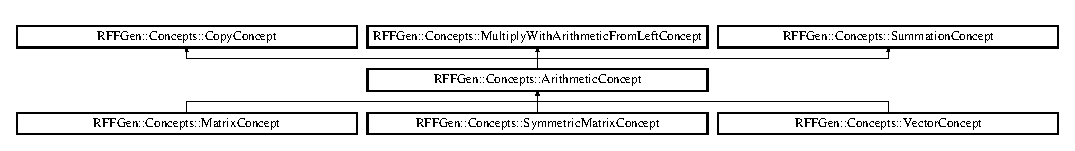
\includegraphics[height=1.586402cm]{structRFFGen_1_1Concepts_1_1ArithmeticConcept}
\end{center}
\end{figure}
\subsection*{Additional Inherited Members}


\subsection{Detailed Description}
Requirements on input types. 

Multiplication between different matrices is not checked here, since this would require to provide all possible matrices to multiply a matrix of type Arg with. 

The documentation for this struct was generated from the following file\-:\begin{DoxyCompactItemize}
\item 
R\-F\-F\-Gen/\hyperlink{concepts_8hh}{concepts.\-hh}\end{DoxyCompactItemize}

\hypertarget{structRFFGen_1_1Concepts_1_1ArithmeticConceptCheck}{\section{R\-F\-F\-Gen\-:\-:Concepts\-:\-:Arithmetic\-Concept\-Check$<$ Arg $>$ Struct Template Reference}
\label{structRFFGen_1_1Concepts_1_1ArithmeticConceptCheck}\index{R\-F\-F\-Gen\-::\-Concepts\-::\-Arithmetic\-Concept\-Check$<$ Arg $>$@{R\-F\-F\-Gen\-::\-Concepts\-::\-Arithmetic\-Concept\-Check$<$ Arg $>$}}
}


Static check if the requirements of \hyperlink{structRFFGen_1_1Concepts_1_1ArithmeticConcept}{Arithmetic\-Concept} are satisfied.  




{\ttfamily \#include $<$concept\-Check.\-hh$>$}

Inheritance diagram for R\-F\-F\-Gen\-:\-:Concepts\-:\-:Arithmetic\-Concept\-Check$<$ Arg $>$\-:\begin{figure}[H]
\begin{center}
\leavevmode
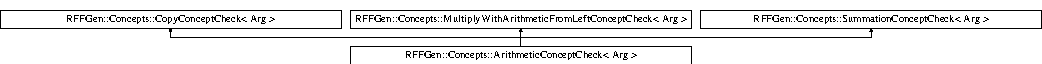
\includegraphics[height=0.860215cm]{structRFFGen_1_1Concepts_1_1ArithmeticConceptCheck}
\end{center}
\end{figure}


\subsection{Detailed Description}
\subsubsection*{template$<$class Arg$>$struct R\-F\-F\-Gen\-::\-Concepts\-::\-Arithmetic\-Concept\-Check$<$ Arg $>$}

Static check if the requirements of \hyperlink{structRFFGen_1_1Concepts_1_1ArithmeticConcept}{Arithmetic\-Concept} are satisfied. 

The documentation for this struct was generated from the following file\-:\begin{DoxyCompactItemize}
\item 
R\-F\-F\-Gen/concept\-Check.\-hh\end{DoxyCompactItemize}

\hypertarget{structRFFGen_1_1CMath_1_1ASin}{\section{R\-F\-F\-Gen\-:\-:C\-Math\-:\-:A\-Sin Struct Reference}
\label{structRFFGen_1_1CMath_1_1ASin}\index{R\-F\-F\-Gen\-::\-C\-Math\-::\-A\-Sin@{R\-F\-F\-Gen\-::\-C\-Math\-::\-A\-Sin}}
}


Sine function including first three derivatives (based on sin(double) in $<$cmath$>$).  




{\ttfamily \#include $<$arcsine.\-hh$>$}

Inheritance diagram for R\-F\-F\-Gen\-:\-:C\-Math\-:\-:A\-Sin\-:\begin{figure}[H]
\begin{center}
\leavevmode
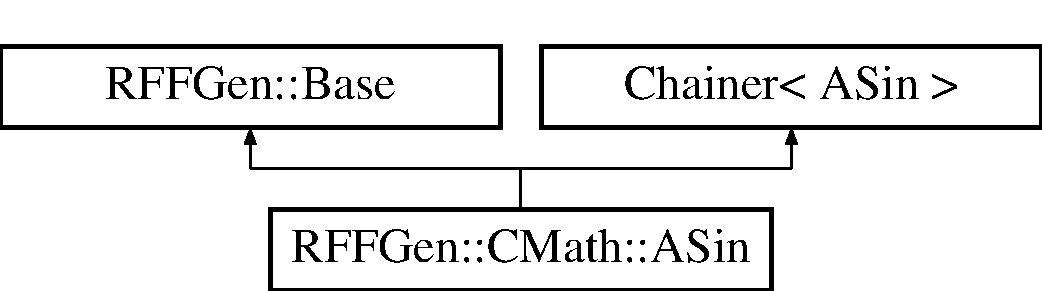
\includegraphics[height=2.000000cm]{structRFFGen_1_1CMath_1_1ASin}
\end{center}
\end{figure}
\subsection*{Public Member Functions}
\begin{DoxyCompactItemize}
\item 
\hyperlink{structRFFGen_1_1CMath_1_1ASin_a06cfb3815955b4f8b3d2627a51064bd8}{A\-Sin} (double x=0.)
\begin{DoxyCompactList}\small\item\em Constructor. \end{DoxyCompactList}\item 
\hypertarget{structRFFGen_1_1CMath_1_1ASin_acab713e2b77c3c3daafe44c62260cb9e}{void \hyperlink{structRFFGen_1_1CMath_1_1ASin_acab713e2b77c3c3daafe44c62260cb9e}{update} (double x)}\label{structRFFGen_1_1CMath_1_1ASin_acab713e2b77c3c3daafe44c62260cb9e}

\begin{DoxyCompactList}\small\item\em Reset point of evaluation. \end{DoxyCompactList}\item 
\hypertarget{structRFFGen_1_1CMath_1_1ASin_abfc89bca232a7dd5ff211eb8c71b6db7}{double \hyperlink{structRFFGen_1_1CMath_1_1ASin_abfc89bca232a7dd5ff211eb8c71b6db7}{d0} () const noexcept}\label{structRFFGen_1_1CMath_1_1ASin_abfc89bca232a7dd5ff211eb8c71b6db7}

\begin{DoxyCompactList}\small\item\em Function value. \end{DoxyCompactList}\item 
\hypertarget{structRFFGen_1_1CMath_1_1ASin_aa7f95c0e1e12b146d2f153e417f0de15}{{\footnotesize template$<$int  = -\/1$>$ }\\double \hyperlink{structRFFGen_1_1CMath_1_1ASin_aa7f95c0e1e12b146d2f153e417f0de15}{d1} (double dx=1) const }\label{structRFFGen_1_1CMath_1_1ASin_aa7f95c0e1e12b146d2f153e417f0de15}

\begin{DoxyCompactList}\small\item\em First (directional) derivative. \end{DoxyCompactList}\item 
\hypertarget{structRFFGen_1_1CMath_1_1ASin_aa4c66cb225c73ae9ce8b1f6a5d86629b}{{\footnotesize template$<$int  = -\/1, int  = -\/1$>$ }\\double \hyperlink{structRFFGen_1_1CMath_1_1ASin_aa4c66cb225c73ae9ce8b1f6a5d86629b}{d2} (double dx=1, double dy=1) const }\label{structRFFGen_1_1CMath_1_1ASin_aa4c66cb225c73ae9ce8b1f6a5d86629b}

\begin{DoxyCompactList}\small\item\em Second (directional) derivative. \end{DoxyCompactList}\item 
\hypertarget{structRFFGen_1_1CMath_1_1ASin_a5492c3159d4bc79df8597f0f3606e4e4}{{\footnotesize template$<$int  = -\/1, int  = -\/1, int  = -\/1$>$ }\\double \hyperlink{structRFFGen_1_1CMath_1_1ASin_a5492c3159d4bc79df8597f0f3606e4e4}{d3} (double dx=1, double dy=1, double dz=1) const }\label{structRFFGen_1_1CMath_1_1ASin_a5492c3159d4bc79df8597f0f3606e4e4}

\begin{DoxyCompactList}\small\item\em Third (directional) derivative. \end{DoxyCompactList}\end{DoxyCompactItemize}


\subsection{Detailed Description}
Sine function including first three derivatives (based on sin(double) in $<$cmath$>$). 

For scalar functions directional derivatives are less interesting. Incorporating this function as building block for more complex functions requires directional derivatives. These occur during applications of the chain rule. 

\subsection{Constructor \& Destructor Documentation}
\hypertarget{structRFFGen_1_1CMath_1_1ASin_a06cfb3815955b4f8b3d2627a51064bd8}{\index{R\-F\-F\-Gen\-::\-C\-Math\-::\-A\-Sin@{R\-F\-F\-Gen\-::\-C\-Math\-::\-A\-Sin}!A\-Sin@{A\-Sin}}
\index{A\-Sin@{A\-Sin}!RFFGen::CMath::ASin@{R\-F\-F\-Gen\-::\-C\-Math\-::\-A\-Sin}}
\subsubsection[{A\-Sin}]{\setlength{\rightskip}{0pt plus 5cm}R\-F\-F\-Gen\-::\-C\-Math\-::\-A\-Sin\-::\-A\-Sin (
\begin{DoxyParamCaption}
\item[{double}]{x = {\ttfamily 0.}}
\end{DoxyParamCaption}
)\hspace{0.3cm}{\ttfamily [inline]}, {\ttfamily [explicit]}}}\label{structRFFGen_1_1CMath_1_1ASin_a06cfb3815955b4f8b3d2627a51064bd8}


Constructor. 


\begin{DoxyParams}{Parameters}
{\em x} & point of evaluation \\
\hline
\end{DoxyParams}


The documentation for this struct was generated from the following file\-:\begin{DoxyCompactItemize}
\item 
R\-F\-F\-Gen/\-C\-Math/arcsine.\-hh\end{DoxyCompactItemize}

\hypertarget{structRFFGen_1_1Base}{\section{R\-F\-F\-Gen\-:\-:Base Struct Reference}
\label{structRFFGen_1_1Base}\index{R\-F\-F\-Gen\-::\-Base@{R\-F\-F\-Gen\-::\-Base}}
}


Base class for functions satisfying Function\-Concept. Required for enabling the operators in \hyperlink{generate_8hh_source}{generate.\-hh}.  




{\ttfamily \#include $<$base.\-hh$>$}

Inheritance diagram for R\-F\-F\-Gen\-:\-:Base\-:\begin{figure}[H]
\begin{center}
\leavevmode
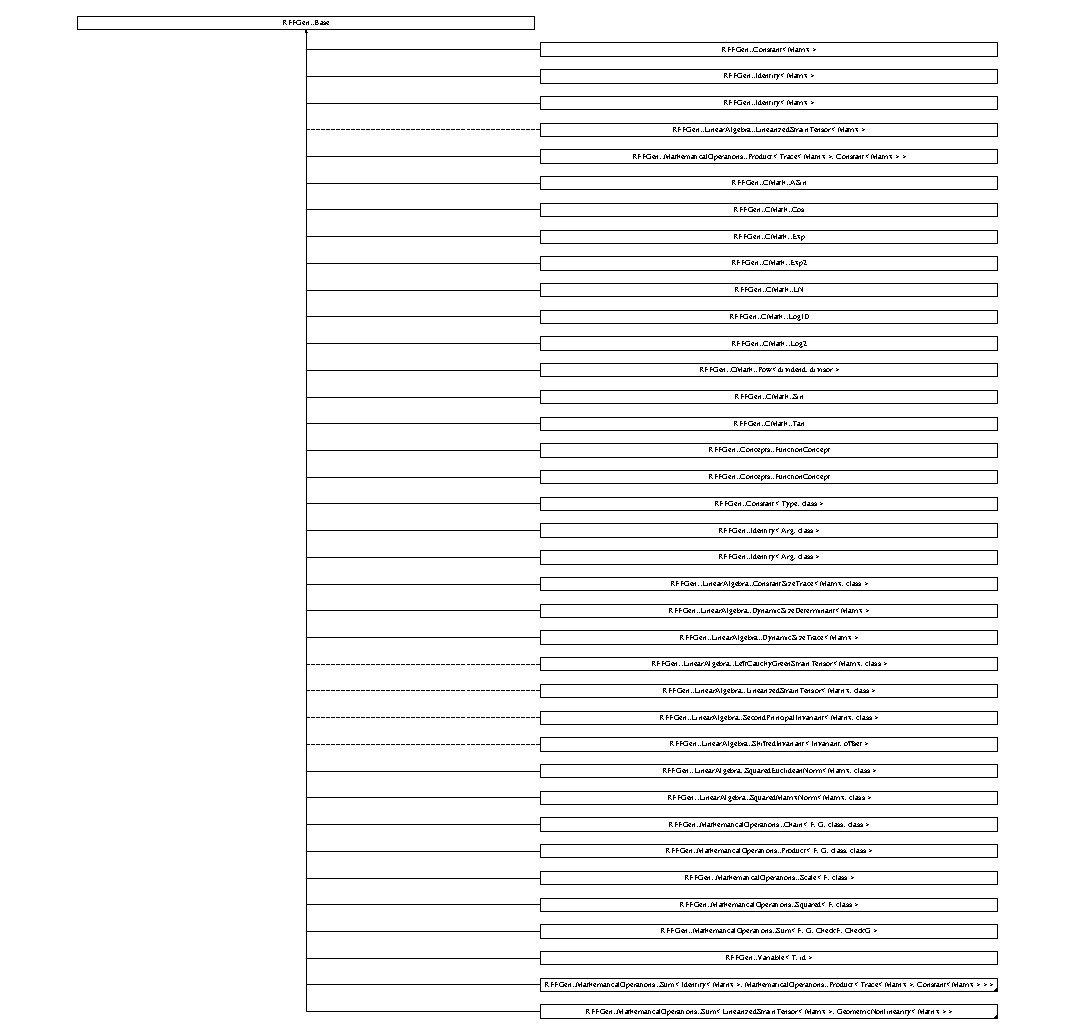
\includegraphics[height=12.000000cm]{structRFFGen_1_1Base}
\end{center}
\end{figure}
\subsection*{Public Member Functions}
\begin{DoxyCompactItemize}
\item 
\hypertarget{structRFFGen_1_1Base_a9b915d8a6df779c47e13cefbaa657c59}{{\footnotesize template$<$class Arg $>$ }\\void \hyperlink{structRFFGen_1_1Base_a9b915d8a6df779c47e13cefbaa657c59}{update} (const Arg \&)}\label{structRFFGen_1_1Base_a9b915d8a6df779c47e13cefbaa657c59}

\begin{DoxyCompactList}\small\item\em Update on changed input. \end{DoxyCompactList}\item 
\hypertarget{structRFFGen_1_1Base_a7e589159c539cc9bf4ebd6ce93ad3ed4}{{\footnotesize template$<$int id, class Arg $>$ }\\void \hyperlink{structRFFGen_1_1Base_a7e589159c539cc9bf4ebd6ce93ad3ed4}{update\-Variable} (const Arg \&)}\label{structRFFGen_1_1Base_a7e589159c539cc9bf4ebd6ce93ad3ed4}

\begin{DoxyCompactList}\small\item\em Empty variables. \end{DoxyCompactList}\end{DoxyCompactItemize}


\subsection{Detailed Description}
Base class for functions satisfying Function\-Concept. Required for enabling the operators in \hyperlink{generate_8hh_source}{generate.\-hh}. 

The documentation for this struct was generated from the following file\-:\begin{DoxyCompactItemize}
\item 
R\-F\-F\-Gen/\-Util/base.\-hh\end{DoxyCompactItemize}

\hypertarget{structRFFGen_1_1MathematicalOperations_1_1Chain}{\section{R\-F\-F\-Gen\-:\-:Mathematical\-Operations\-:\-:Chain$<$ F, G, class, class $>$ Struct Template Reference}
\label{structRFFGen_1_1MathematicalOperations_1_1Chain}\index{R\-F\-F\-Gen\-::\-Mathematical\-Operations\-::\-Chain$<$ F, G, class, class $>$@{R\-F\-F\-Gen\-::\-Mathematical\-Operations\-::\-Chain$<$ F, G, class, class $>$}}
}


Chain $ f\circ g $ of functions $f$ and $g$ of type F resp. G (F and G must satisfy the requirements of \hyperlink{structRFFGen_1_1Concepts_1_1FunctionConcept}{Concepts\-::\-Function\-Concept}).  




{\ttfamily \#include $<$chain.\-hh$>$}

Inheritance diagram for R\-F\-F\-Gen\-:\-:Mathematical\-Operations\-:\-:Chain$<$ F, G, class, class $>$\-:\begin{figure}[H]
\begin{center}
\leavevmode
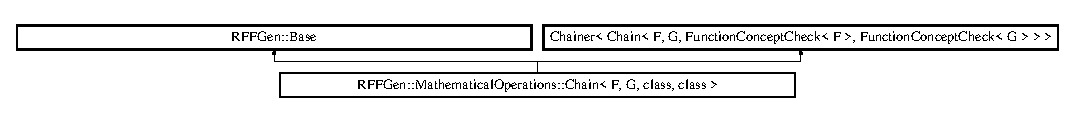
\includegraphics[height=0.979021cm]{structRFFGen_1_1MathematicalOperations_1_1Chain}
\end{center}
\end{figure}
\subsection*{Public Member Functions}
\begin{DoxyCompactItemize}
\item 
\hypertarget{structRFFGen_1_1MathematicalOperations_1_1Chain_aebcae20e7b869fcaa9ec1039b3de8fd5}{\hyperlink{structRFFGen_1_1MathematicalOperations_1_1Chain_aebcae20e7b869fcaa9ec1039b3de8fd5}{Chain} ()=default}\label{structRFFGen_1_1MathematicalOperations_1_1Chain_aebcae20e7b869fcaa9ec1039b3de8fd5}

\begin{DoxyCompactList}\small\item\em Default constructor. May leave member variables uninitialized! Call update before using evaluation. \end{DoxyCompactList}\item 
{\footnotesize template$<$class... Init\-Function$>$ }\\\hyperlink{structRFFGen_1_1MathematicalOperations_1_1Chain_a9d891fe5b5e9bfc7af6c87d2b6dd0731}{Chain} (const Init\-Function \&...init)
\begin{DoxyCompactList}\small\item\em Constructor. \end{DoxyCompactList}\item 
\hyperlink{structRFFGen_1_1MathematicalOperations_1_1Chain_a313e8d55e65802fdcbbd03619dbe3bf2}{Chain} (const F \&f\-\_\-, const G \&g\-\_\-)
\begin{DoxyCompactList}\small\item\em Constructor taking copies of the functions to be chained. \end{DoxyCompactList}\item 
\hypertarget{structRFFGen_1_1MathematicalOperations_1_1Chain_aa2e25c8560d0383e0b07a1886fc92077}{{\footnotesize template$<$class Arg $>$ }\\void \hyperlink{structRFFGen_1_1MathematicalOperations_1_1Chain_aa2e25c8560d0383e0b07a1886fc92077}{update} (const Arg \&x)}\label{structRFFGen_1_1MathematicalOperations_1_1Chain_aa2e25c8560d0383e0b07a1886fc92077}

\begin{DoxyCompactList}\small\item\em Reset point of evaluation. \end{DoxyCompactList}\item 
\hypertarget{structRFFGen_1_1MathematicalOperations_1_1Chain_a6b9577d631eb244c76d7b3d3f3d993d7}{{\footnotesize template$<$int index, class Arg $>$ }\\void \hyperlink{structRFFGen_1_1MathematicalOperations_1_1Chain_a6b9577d631eb244c76d7b3d3f3d993d7}{update\-Variable} (const Arg \&x)}\label{structRFFGen_1_1MathematicalOperations_1_1Chain_a6b9577d631eb244c76d7b3d3f3d993d7}

\begin{DoxyCompactList}\small\item\em Propagate call to \hyperlink{structRFFGen_1_1MathematicalOperations_1_1Chain_a6b9577d631eb244c76d7b3d3f3d993d7}{update\-Variable()} to f and g. \end{DoxyCompactList}\item 
\hypertarget{structRFFGen_1_1MathematicalOperations_1_1Chain_aac13e9d28dc10dff07fa40c33b43309f}{const auto \& \hyperlink{structRFFGen_1_1MathematicalOperations_1_1Chain_aac13e9d28dc10dff07fa40c33b43309f}{d0} () const noexcept}\label{structRFFGen_1_1MathematicalOperations_1_1Chain_aac13e9d28dc10dff07fa40c33b43309f}

\begin{DoxyCompactList}\small\item\em Function value. \end{DoxyCompactList}\item 
{\footnotesize template$<$int id, class Arg , class Indexed\-Arg  = Indexed\-Type$<$\-Arg,id$>$, class Indexed\-F\-Arg  = Indexed\-Type$<$\-F\-Arg,id$>$, class  = std\-::enable\-\_\-if\-\_\-t$<$ Compute\-Chain\-D1$<$ F , D1$<$\-G,\-Indexed\-Arg$>$ , Indexed\-F\-Arg $>$\-::present$>$$>$ }\\auto \hyperlink{structRFFGen_1_1MathematicalOperations_1_1Chain_ac762868ce03eb3089f3cd1943062f9a2}{d1} (Arg const \&dx) const 
\begin{DoxyCompactList}\small\item\em First directional derivative. \end{DoxyCompactList}\item 
{\footnotesize template$<$int idx, int idy, class Arg\-X , class Arg\-Y , class Indexed\-Arg\-X  = Indexed\-Type$<$\-Arg\-X,idx$>$, class Indexed\-Arg\-Y  = Indexed\-Type$<$\-Arg\-Y,idy$>$, class Indexed\-F\-Arg\-X  = Indexed\-Type$<$\-F\-Arg,idx$>$, class Indexed\-F\-Arg\-Y  = Indexed\-Type$<$\-F\-Arg,idy$>$, class  = std\-::enable\-\_\-if\-\_\-t$<$ D2\-Lazy\-Type$<$\-Indexed\-Arg\-X,\-Indexed\-Arg\-Y,\-Indexed\-F\-Arg\-X,\-Indexed\-F\-Arg\-Y$>$\-::present $>$$>$ }\\auto \hyperlink{structRFFGen_1_1MathematicalOperations_1_1Chain_ad1fd27be6286cadf63fff93595b83c46}{d2} (Arg\-X const \&dx, Arg\-Y const \&dy) const 
\begin{DoxyCompactList}\small\item\em Second directional derivative. \end{DoxyCompactList}\item 
{\footnotesize template$<$int idx, int idy, int idz, class Arg\-X , class Arg\-Y , class Arg\-Z , class Indexed\-Arg\-X  = Indexed\-Type$<$\-Arg\-X,idx$>$, class Indexed\-Arg\-Y  = Indexed\-Type$<$\-Arg\-Y,idy$>$, class Indexed\-Arg\-Z  = Indexed\-Type$<$\-Arg\-Z,idz$>$, class Indexed\-F\-Arg\-X  = Indexed\-Type$<$\-F\-Arg,idx$>$, class Indexed\-F\-Arg\-Y  = Indexed\-Type$<$\-F\-Arg,idy$>$, class Indexed\-F\-Arg\-Z  = Indexed\-Type$<$\-F\-Arg,idz$>$, class  = std\-::enable\-\_\-if\-\_\-t$<$ D3\-Lazy\-Type$<$\-Indexed\-Arg\-X,\-Indexed\-Arg\-Y,\-Indexed\-Arg\-Z,\-Indexed\-F\-Arg\-X,\-Indexed\-F\-Arg\-Y,\-Indexed\-F\-Arg\-Z$>$\-::present $>$$>$ }\\auto \hyperlink{structRFFGen_1_1MathematicalOperations_1_1Chain_a9c99a40bc32fe065acd3144f3d6a4ce7}{d3} (Arg\-X const \&dx, Arg\-Y const \&dy, Arg\-Z const \&dz) const 
\begin{DoxyCompactList}\small\item\em Third directional derivative. \end{DoxyCompactList}\end{DoxyCompactItemize}


\subsection{Detailed Description}
\subsubsection*{template$<$class F, class G, class = Function\-Concept\-Check$<$\-F$>$, class = Function\-Concept\-Check$<$\-G$>$$>$struct R\-F\-F\-Gen\-::\-Mathematical\-Operations\-::\-Chain$<$ F, G, class, class $>$}

Chain $ f\circ g $ of functions $f$ and $g$ of type F resp. G (F and G must satisfy the requirements of \hyperlink{structRFFGen_1_1Concepts_1_1FunctionConcept}{Concepts\-::\-Function\-Concept}). 

\subsection{Constructor \& Destructor Documentation}
\hypertarget{structRFFGen_1_1MathematicalOperations_1_1Chain_a9d891fe5b5e9bfc7af6c87d2b6dd0731}{\index{R\-F\-F\-Gen\-::\-Mathematical\-Operations\-::\-Chain@{R\-F\-F\-Gen\-::\-Mathematical\-Operations\-::\-Chain}!Chain@{Chain}}
\index{Chain@{Chain}!RFFGen::MathematicalOperations::Chain@{R\-F\-F\-Gen\-::\-Mathematical\-Operations\-::\-Chain}}
\subsubsection[{Chain}]{\setlength{\rightskip}{0pt plus 5cm}template$<$class F, class G, class  = Function\-Concept\-Check$<$\-F$>$, class  = Function\-Concept\-Check$<$\-G$>$$>$ template$<$class... Init\-Function$>$ {\bf R\-F\-F\-Gen\-::\-Mathematical\-Operations\-::\-Chain}$<$ F, G, class, class $>$\-::{\bf Chain} (
\begin{DoxyParamCaption}
\item[{const Init\-Function \&...}]{init}
\end{DoxyParamCaption}
)\hspace{0.3cm}{\ttfamily [inline]}}}\label{structRFFGen_1_1MathematicalOperations_1_1Chain_a9d891fe5b5e9bfc7af6c87d2b6dd0731}


Constructor. 


\begin{DoxyParams}{Parameters}
{\em init} & input for a constructor of G \\
\hline
\end{DoxyParams}
\hypertarget{structRFFGen_1_1MathematicalOperations_1_1Chain_a313e8d55e65802fdcbbd03619dbe3bf2}{\index{R\-F\-F\-Gen\-::\-Mathematical\-Operations\-::\-Chain@{R\-F\-F\-Gen\-::\-Mathematical\-Operations\-::\-Chain}!Chain@{Chain}}
\index{Chain@{Chain}!RFFGen::MathematicalOperations::Chain@{R\-F\-F\-Gen\-::\-Mathematical\-Operations\-::\-Chain}}
\subsubsection[{Chain}]{\setlength{\rightskip}{0pt plus 5cm}template$<$class F, class G, class  = Function\-Concept\-Check$<$\-F$>$, class  = Function\-Concept\-Check$<$\-G$>$$>$ {\bf R\-F\-F\-Gen\-::\-Mathematical\-Operations\-::\-Chain}$<$ F, G, class, class $>$\-::{\bf Chain} (
\begin{DoxyParamCaption}
\item[{const F \&}]{f\-\_\-, }
\item[{const G \&}]{g\-\_\-}
\end{DoxyParamCaption}
)\hspace{0.3cm}{\ttfamily [inline]}}}\label{structRFFGen_1_1MathematicalOperations_1_1Chain_a313e8d55e65802fdcbbd03619dbe3bf2}


Constructor taking copies of the functions to be chained. 


\begin{DoxyParams}{Parameters}
{\em f\-\_\-} & outer function \\
\hline
{\em g\-\_\-} & inner function \\
\hline
\end{DoxyParams}


\subsection{Member Function Documentation}
\hypertarget{structRFFGen_1_1MathematicalOperations_1_1Chain_ac762868ce03eb3089f3cd1943062f9a2}{\index{R\-F\-F\-Gen\-::\-Mathematical\-Operations\-::\-Chain@{R\-F\-F\-Gen\-::\-Mathematical\-Operations\-::\-Chain}!d1@{d1}}
\index{d1@{d1}!RFFGen::MathematicalOperations::Chain@{R\-F\-F\-Gen\-::\-Mathematical\-Operations\-::\-Chain}}
\subsubsection[{d1}]{\setlength{\rightskip}{0pt plus 5cm}template$<$class F, class G, class  = Function\-Concept\-Check$<$\-F$>$, class  = Function\-Concept\-Check$<$\-G$>$$>$ template$<$int id, class Arg , class Indexed\-Arg  = Indexed\-Type$<$\-Arg,id$>$, class Indexed\-F\-Arg  = Indexed\-Type$<$\-F\-Arg,id$>$, class  = std\-::enable\-\_\-if\-\_\-t$<$ Compute\-Chain\-D1$<$ F , D1$<$\-G,\-Indexed\-Arg$>$ , Indexed\-F\-Arg $>$\-::present$>$$>$ auto {\bf R\-F\-F\-Gen\-::\-Mathematical\-Operations\-::\-Chain}$<$ F, G, class, class $>$\-::d1 (
\begin{DoxyParamCaption}
\item[{Arg const \&}]{dx}
\end{DoxyParamCaption}
) const\hspace{0.3cm}{\ttfamily [inline]}}}\label{structRFFGen_1_1MathematicalOperations_1_1Chain_ac762868ce03eb3089f3cd1943062f9a2}


First directional derivative. 


\begin{DoxyParams}{Parameters}
{\em dx} & direction for which the derivative is computed \\
\hline
\end{DoxyParams}
\hypertarget{structRFFGen_1_1MathematicalOperations_1_1Chain_ad1fd27be6286cadf63fff93595b83c46}{\index{R\-F\-F\-Gen\-::\-Mathematical\-Operations\-::\-Chain@{R\-F\-F\-Gen\-::\-Mathematical\-Operations\-::\-Chain}!d2@{d2}}
\index{d2@{d2}!RFFGen::MathematicalOperations::Chain@{R\-F\-F\-Gen\-::\-Mathematical\-Operations\-::\-Chain}}
\subsubsection[{d2}]{\setlength{\rightskip}{0pt plus 5cm}template$<$class F, class G, class  = Function\-Concept\-Check$<$\-F$>$, class  = Function\-Concept\-Check$<$\-G$>$$>$ template$<$int idx, int idy, class Arg\-X , class Arg\-Y , class Indexed\-Arg\-X  = Indexed\-Type$<$\-Arg\-X,idx$>$, class Indexed\-Arg\-Y  = Indexed\-Type$<$\-Arg\-Y,idy$>$, class Indexed\-F\-Arg\-X  = Indexed\-Type$<$\-F\-Arg,idx$>$, class Indexed\-F\-Arg\-Y  = Indexed\-Type$<$\-F\-Arg,idy$>$, class  = std\-::enable\-\_\-if\-\_\-t$<$ D2\-Lazy\-Type$<$\-Indexed\-Arg\-X,\-Indexed\-Arg\-Y,\-Indexed\-F\-Arg\-X,\-Indexed\-F\-Arg\-Y$>$\-::present $>$$>$ auto {\bf R\-F\-F\-Gen\-::\-Mathematical\-Operations\-::\-Chain}$<$ F, G, class, class $>$\-::d2 (
\begin{DoxyParamCaption}
\item[{Arg\-X const \&}]{dx, }
\item[{Arg\-Y const \&}]{dy}
\end{DoxyParamCaption}
) const\hspace{0.3cm}{\ttfamily [inline]}}}\label{structRFFGen_1_1MathematicalOperations_1_1Chain_ad1fd27be6286cadf63fff93595b83c46}


Second directional derivative. 


\begin{DoxyParams}{Parameters}
{\em dx} & direction for which the derivative is computed \\
\hline
{\em dy} & direction for which the derivative is computed \\
\hline
\end{DoxyParams}
\hypertarget{structRFFGen_1_1MathematicalOperations_1_1Chain_a9c99a40bc32fe065acd3144f3d6a4ce7}{\index{R\-F\-F\-Gen\-::\-Mathematical\-Operations\-::\-Chain@{R\-F\-F\-Gen\-::\-Mathematical\-Operations\-::\-Chain}!d3@{d3}}
\index{d3@{d3}!RFFGen::MathematicalOperations::Chain@{R\-F\-F\-Gen\-::\-Mathematical\-Operations\-::\-Chain}}
\subsubsection[{d3}]{\setlength{\rightskip}{0pt plus 5cm}template$<$class F, class G, class  = Function\-Concept\-Check$<$\-F$>$, class  = Function\-Concept\-Check$<$\-G$>$$>$ template$<$int idx, int idy, int idz, class Arg\-X , class Arg\-Y , class Arg\-Z , class Indexed\-Arg\-X  = Indexed\-Type$<$\-Arg\-X,idx$>$, class Indexed\-Arg\-Y  = Indexed\-Type$<$\-Arg\-Y,idy$>$, class Indexed\-Arg\-Z  = Indexed\-Type$<$\-Arg\-Z,idz$>$, class Indexed\-F\-Arg\-X  = Indexed\-Type$<$\-F\-Arg,idx$>$, class Indexed\-F\-Arg\-Y  = Indexed\-Type$<$\-F\-Arg,idy$>$, class Indexed\-F\-Arg\-Z  = Indexed\-Type$<$\-F\-Arg,idz$>$, class  = std\-::enable\-\_\-if\-\_\-t$<$ D3\-Lazy\-Type$<$\-Indexed\-Arg\-X,\-Indexed\-Arg\-Y,\-Indexed\-Arg\-Z,\-Indexed\-F\-Arg\-X,\-Indexed\-F\-Arg\-Y,\-Indexed\-F\-Arg\-Z$>$\-::present $>$$>$ auto {\bf R\-F\-F\-Gen\-::\-Mathematical\-Operations\-::\-Chain}$<$ F, G, class, class $>$\-::d3 (
\begin{DoxyParamCaption}
\item[{Arg\-X const \&}]{dx, }
\item[{Arg\-Y const \&}]{dy, }
\item[{Arg\-Z const \&}]{dz}
\end{DoxyParamCaption}
) const\hspace{0.3cm}{\ttfamily [inline]}}}\label{structRFFGen_1_1MathematicalOperations_1_1Chain_a9c99a40bc32fe065acd3144f3d6a4ce7}


Third directional derivative. 


\begin{DoxyParams}{Parameters}
{\em dx} & direction for which the derivative is computed \\
\hline
{\em dy} & direction for which the derivative is computed \\
\hline
{\em dz} & direction for which the derivative is computed \\
\hline
\end{DoxyParams}


The documentation for this struct was generated from the following file\-:\begin{DoxyCompactItemize}
\item 
R\-F\-F\-Gen/\-Mathematical\-Operations/chain.\-hh\end{DoxyCompactItemize}

\hypertarget{structRFFGen_1_1Chainer}{\section{R\-F\-F\-Gen\-:\-:Chainer$<$ class $>$ Struct Template Reference}
\label{structRFFGen_1_1Chainer}\index{R\-F\-F\-Gen\-::\-Chainer$<$ class $>$@{R\-F\-F\-Gen\-::\-Chainer$<$ class $>$}}
}


The documentation for this struct was generated from the following file\-:\begin{DoxyCompactItemize}
\item 
R\-F\-F\-Gen/\-Mathematical\-Operations/sum.\-hh\end{DoxyCompactItemize}

\hypertarget{structRFFGen_1_1Constant}{\section{R\-F\-F\-Gen\-:\-:Constant$<$ Type, class $>$ Struct Template Reference}
\label{structRFFGen_1_1Constant}\index{R\-F\-F\-Gen\-::\-Constant$<$ Type, class $>$@{R\-F\-F\-Gen\-::\-Constant$<$ Type, class $>$}}
}


Wrap a constant.  




{\ttfamily \#include $<$constant.\-hh$>$}

Inheritance diagram for R\-F\-F\-Gen\-:\-:Constant$<$ Type, class $>$\-:\begin{figure}[H]
\begin{center}
\leavevmode
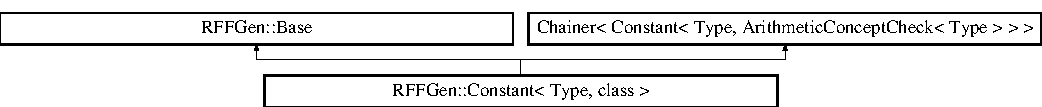
\includegraphics[height=1.435897cm]{structRFFGen_1_1Constant}
\end{center}
\end{figure}
\subsection*{Public Member Functions}
\begin{DoxyCompactItemize}
\item 
\hypertarget{structRFFGen_1_1Constant_ae2d0e64d773d967430d13e47817d6d84}{\hyperlink{structRFFGen_1_1Constant_ae2d0e64d773d967430d13e47817d6d84}{Constant} (Type const \&t\-\_\-)}\label{structRFFGen_1_1Constant_ae2d0e64d773d967430d13e47817d6d84}

\begin{DoxyCompactList}\small\item\em Construct constant from copy. \end{DoxyCompactList}\item 
\hypertarget{structRFFGen_1_1Constant_a185f8aa750fe120dbe255de11107b7e1}{const Type \& \hyperlink{structRFFGen_1_1Constant_a185f8aa750fe120dbe255de11107b7e1}{d0} () const noexcept}\label{structRFFGen_1_1Constant_a185f8aa750fe120dbe255de11107b7e1}

\begin{DoxyCompactList}\small\item\em Function value. \end{DoxyCompactList}\end{DoxyCompactItemize}


\subsection{Detailed Description}
\subsubsection*{template$<$class Type, class = Arithmetic\-Concept\-Check$<$\-Type$>$$>$struct R\-F\-F\-Gen\-::\-Constant$<$ Type, class $>$}

Wrap a constant. 

The documentation for this struct was generated from the following file\-:\begin{DoxyCompactItemize}
\item 
R\-F\-F\-Gen/constant.\-hh\end{DoxyCompactItemize}

\hypertarget{structRFFGen_1_1LinearAlgebra_1_1ConstantSizeTrace}{\section{R\-F\-F\-Gen\-:\-:Linear\-Algebra\-:\-:Constant\-Size\-Trace$<$ Matrix, class $>$ Struct Template Reference}
\label{structRFFGen_1_1LinearAlgebra_1_1ConstantSizeTrace}\index{R\-F\-F\-Gen\-::\-Linear\-Algebra\-::\-Constant\-Size\-Trace$<$ Matrix, class $>$@{R\-F\-F\-Gen\-::\-Linear\-Algebra\-::\-Constant\-Size\-Trace$<$ Matrix, class $>$}}
}


Trace of a matrix, i.\-e. sum of diagonal elements.  




{\ttfamily \#include $<$trace.\-hh$>$}

Inheritance diagram for R\-F\-F\-Gen\-:\-:Linear\-Algebra\-:\-:Constant\-Size\-Trace$<$ Matrix, class $>$\-:\begin{figure}[H]
\begin{center}
\leavevmode
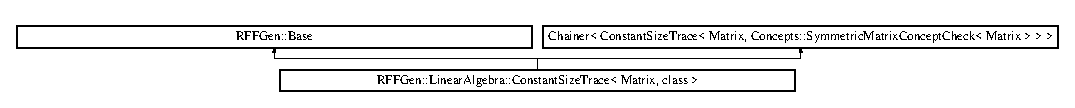
\includegraphics[height=1.005386cm]{structRFFGen_1_1LinearAlgebra_1_1ConstantSizeTrace}
\end{center}
\end{figure}
\subsection*{Public Member Functions}
\begin{DoxyCompactItemize}
\item 
\hypertarget{structRFFGen_1_1LinearAlgebra_1_1ConstantSizeTrace_a54bd89f9dbd5b2aa1845859b265571d4}{\hyperlink{structRFFGen_1_1LinearAlgebra_1_1ConstantSizeTrace_a54bd89f9dbd5b2aa1845859b265571d4}{Constant\-Size\-Trace} ()=default}\label{structRFFGen_1_1LinearAlgebra_1_1ConstantSizeTrace_a54bd89f9dbd5b2aa1845859b265571d4}

\begin{DoxyCompactList}\small\item\em Default constructor. \end{DoxyCompactList}\item 
\hyperlink{structRFFGen_1_1LinearAlgebra_1_1ConstantSizeTrace_a9ed61eb129e946f682dcbb7e5bd0b028}{Constant\-Size\-Trace} (const Matrix \&A)
\begin{DoxyCompactList}\small\item\em Constructor. \end{DoxyCompactList}\item 
\hypertarget{structRFFGen_1_1LinearAlgebra_1_1ConstantSizeTrace_abf6e90e249fbdaf4be00b9c155989ab0}{void \hyperlink{structRFFGen_1_1LinearAlgebra_1_1ConstantSizeTrace_abf6e90e249fbdaf4be00b9c155989ab0}{update} (const Matrix \&A)}\label{structRFFGen_1_1LinearAlgebra_1_1ConstantSizeTrace_abf6e90e249fbdaf4be00b9c155989ab0}

\begin{DoxyCompactList}\small\item\em Reset point of evaluation. \end{DoxyCompactList}\item 
\hypertarget{structRFFGen_1_1LinearAlgebra_1_1ConstantSizeTrace_a932aa99cd77b7f4c53cbebb8982a5056}{const auto \& \hyperlink{structRFFGen_1_1LinearAlgebra_1_1ConstantSizeTrace_a932aa99cd77b7f4c53cbebb8982a5056}{operator()} () const noexcept}\label{structRFFGen_1_1LinearAlgebra_1_1ConstantSizeTrace_a932aa99cd77b7f4c53cbebb8982a5056}

\begin{DoxyCompactList}\small\item\em Function value. Convenient access to d0. \end{DoxyCompactList}\item 
\hypertarget{structRFFGen_1_1LinearAlgebra_1_1ConstantSizeTrace_ac23921eac39533680c9060865728ab5c}{const auto \& \hyperlink{structRFFGen_1_1LinearAlgebra_1_1ConstantSizeTrace_ac23921eac39533680c9060865728ab5c}{operator()} (const Matrix \&A) const }\label{structRFFGen_1_1LinearAlgebra_1_1ConstantSizeTrace_ac23921eac39533680c9060865728ab5c}

\begin{DoxyCompactList}\small\item\em Function value. Convenient access to d0 with prior call to update(\-A). \end{DoxyCompactList}\item 
\hypertarget{structRFFGen_1_1LinearAlgebra_1_1ConstantSizeTrace_a5a96a8d7a1adbbb5f5e22e7f6a26727b}{const auto \& \hyperlink{structRFFGen_1_1LinearAlgebra_1_1ConstantSizeTrace_a5a96a8d7a1adbbb5f5e22e7f6a26727b}{d0} () const noexcept}\label{structRFFGen_1_1LinearAlgebra_1_1ConstantSizeTrace_a5a96a8d7a1adbbb5f5e22e7f6a26727b}

\begin{DoxyCompactList}\small\item\em Function value. \end{DoxyCompactList}\item 
\hypertarget{structRFFGen_1_1LinearAlgebra_1_1ConstantSizeTrace_a3d21fef989ae6d57cf64a282a8ee4cd0}{{\footnotesize template$<$int $>$ }\\auto \hyperlink{structRFFGen_1_1LinearAlgebra_1_1ConstantSizeTrace_a3d21fef989ae6d57cf64a282a8ee4cd0}{d1} (const Matrix \&d\-A) const }\label{structRFFGen_1_1LinearAlgebra_1_1ConstantSizeTrace_a3d21fef989ae6d57cf64a282a8ee4cd0}

\begin{DoxyCompactList}\small\item\em First directional derivative. \end{DoxyCompactList}\end{DoxyCompactItemize}


\subsection{Detailed Description}
\subsubsection*{template$<$class Matrix, class = Concepts\-::\-Symmetric\-Matrix\-Concept\-Check$<$\-Matrix$>$$>$struct R\-F\-F\-Gen\-::\-Linear\-Algebra\-::\-Constant\-Size\-Trace$<$ Matrix, class $>$}

Trace of a matrix, i.\-e. sum of diagonal elements. 

\subsection{Constructor \& Destructor Documentation}
\hypertarget{structRFFGen_1_1LinearAlgebra_1_1ConstantSizeTrace_a9ed61eb129e946f682dcbb7e5bd0b028}{\index{R\-F\-F\-Gen\-::\-Linear\-Algebra\-::\-Constant\-Size\-Trace@{R\-F\-F\-Gen\-::\-Linear\-Algebra\-::\-Constant\-Size\-Trace}!Constant\-Size\-Trace@{Constant\-Size\-Trace}}
\index{Constant\-Size\-Trace@{Constant\-Size\-Trace}!RFFGen::LinearAlgebra::ConstantSizeTrace@{R\-F\-F\-Gen\-::\-Linear\-Algebra\-::\-Constant\-Size\-Trace}}
\subsubsection[{Constant\-Size\-Trace}]{\setlength{\rightskip}{0pt plus 5cm}template$<$class Matrix , class  = Concepts\-::\-Symmetric\-Matrix\-Concept\-Check$<$\-Matrix$>$$>$ {\bf R\-F\-F\-Gen\-::\-Linear\-Algebra\-::\-Constant\-Size\-Trace}$<$ Matrix, class $>$\-::{\bf Constant\-Size\-Trace} (
\begin{DoxyParamCaption}
\item[{const Matrix \&}]{A}
\end{DoxyParamCaption}
)\hspace{0.3cm}{\ttfamily [inline]}, {\ttfamily [explicit]}}}\label{structRFFGen_1_1LinearAlgebra_1_1ConstantSizeTrace_a9ed61eb129e946f682dcbb7e5bd0b028}


Constructor. 


\begin{DoxyParams}{Parameters}
{\em A} & point of evaluation. \\
\hline
\end{DoxyParams}


The documentation for this struct was generated from the following file\-:\begin{DoxyCompactItemize}
\item 
R\-F\-F\-Gen/\-Linear\-Algebra/trace.\-hh\end{DoxyCompactItemize}

\hypertarget{structRFFGen_1_1Concepts_1_1CopyConcept}{\section{R\-F\-F\-Gen\-:\-:Concepts\-:\-:Copy\-Concept Struct Reference}
\label{structRFFGen_1_1Concepts_1_1CopyConcept}\index{R\-F\-F\-Gen\-::\-Concepts\-::\-Copy\-Concept@{R\-F\-F\-Gen\-::\-Concepts\-::\-Copy\-Concept}}
}


Requires copy-\/constructibility and copy-\/assignability.  




{\ttfamily \#include $<$concepts.\-hh$>$}

Inheritance diagram for R\-F\-F\-Gen\-:\-:Concepts\-:\-:Copy\-Concept\-:\begin{figure}[H]
\begin{center}
\leavevmode
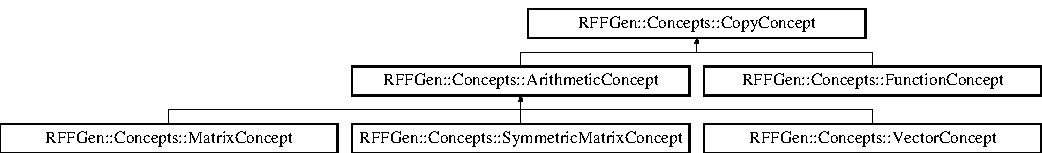
\includegraphics[height=2.058824cm]{structRFFGen_1_1Concepts_1_1CopyConcept}
\end{center}
\end{figure}
\subsection*{Public Member Functions}
\begin{DoxyCompactItemize}
\item 
\hypertarget{structRFFGen_1_1Concepts_1_1CopyConcept_a8c65652314ce23b53ff82ff5c1e6d7a2}{\hyperlink{structRFFGen_1_1Concepts_1_1CopyConcept_a8c65652314ce23b53ff82ff5c1e6d7a2}{Copy\-Concept} (const \hyperlink{structRFFGen_1_1Concepts_1_1CopyConcept}{Copy\-Concept} \&)}\label{structRFFGen_1_1Concepts_1_1CopyConcept_a8c65652314ce23b53ff82ff5c1e6d7a2}

\begin{DoxyCompactList}\small\item\em Copy-\/constructible. \end{DoxyCompactList}\item 
\hypertarget{structRFFGen_1_1Concepts_1_1CopyConcept_a14e42cfa42f78c5142bd51b24e9056bc}{\hyperlink{structRFFGen_1_1Concepts_1_1CopyConcept}{Copy\-Concept} \& \hyperlink{structRFFGen_1_1Concepts_1_1CopyConcept_a14e42cfa42f78c5142bd51b24e9056bc}{operator=} (const \hyperlink{structRFFGen_1_1Concepts_1_1CopyConcept}{Copy\-Concept} \&)}\label{structRFFGen_1_1Concepts_1_1CopyConcept_a14e42cfa42f78c5142bd51b24e9056bc}

\begin{DoxyCompactList}\small\item\em Copy-\/assignable. \end{DoxyCompactList}\end{DoxyCompactItemize}


\subsection{Detailed Description}
Requires copy-\/constructibility and copy-\/assignability. 

The documentation for this struct was generated from the following file\-:\begin{DoxyCompactItemize}
\item 
R\-F\-F\-Gen/\hyperlink{concepts_8hh}{concepts.\-hh}\end{DoxyCompactItemize}

\hypertarget{structRFFGen_1_1Concepts_1_1CopyConceptCheck}{\section{R\-F\-F\-Gen\-:\-:Concepts\-:\-:Copy\-Concept\-Check$<$ Arg $>$ Struct Template Reference}
\label{structRFFGen_1_1Concepts_1_1CopyConceptCheck}\index{R\-F\-F\-Gen\-::\-Concepts\-::\-Copy\-Concept\-Check$<$ Arg $>$@{R\-F\-F\-Gen\-::\-Concepts\-::\-Copy\-Concept\-Check$<$ Arg $>$}}
}


Static check if the requirements of \hyperlink{structRFFGen_1_1Concepts_1_1CopyConcept}{Copy\-Concept} are satisfied.  




{\ttfamily \#include $<$concept\-Check.\-hh$>$}

Inheritance diagram for R\-F\-F\-Gen\-:\-:Concepts\-:\-:Copy\-Concept\-Check$<$ Arg $>$\-:\begin{figure}[H]
\begin{center}
\leavevmode
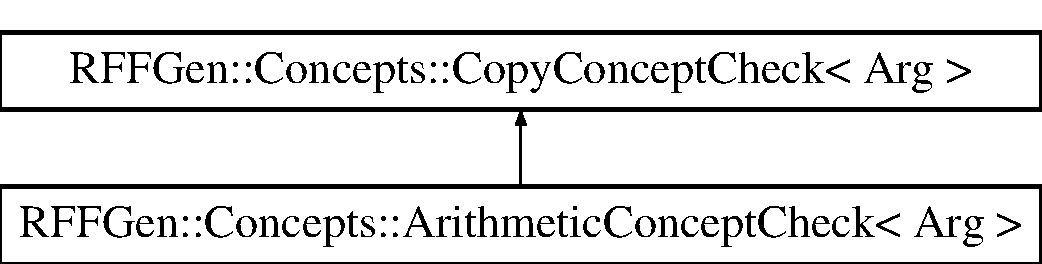
\includegraphics[height=2.000000cm]{structRFFGen_1_1Concepts_1_1CopyConceptCheck}
\end{center}
\end{figure}


\subsection{Detailed Description}
\subsubsection*{template$<$class Arg$>$struct R\-F\-F\-Gen\-::\-Concepts\-::\-Copy\-Concept\-Check$<$ Arg $>$}

Static check if the requirements of \hyperlink{structRFFGen_1_1Concepts_1_1CopyConcept}{Copy\-Concept} are satisfied. 


\begin{DoxyTemplParams}{Template Parameters}
{\em Arg} & type to check \\
\hline
\end{DoxyTemplParams}


The documentation for this struct was generated from the following file\-:\begin{DoxyCompactItemize}
\item 
R\-F\-F\-Gen/concept\-Check.\-hh\end{DoxyCompactItemize}

\hypertarget{structRFFGen_1_1CMath_1_1Cos}{\section{R\-F\-F\-Gen\-:\-:C\-Math\-:\-:Cos Struct Reference}
\label{structRFFGen_1_1CMath_1_1Cos}\index{R\-F\-F\-Gen\-::\-C\-Math\-::\-Cos@{R\-F\-F\-Gen\-::\-C\-Math\-::\-Cos}}
}


Cosine function including first three derivatives (based on cos(double) in $<$cmath$>$).  




{\ttfamily \#include $<$cosine.\-hh$>$}

Inheritance diagram for R\-F\-F\-Gen\-:\-:C\-Math\-:\-:Cos\-:\begin{figure}[H]
\begin{center}
\leavevmode
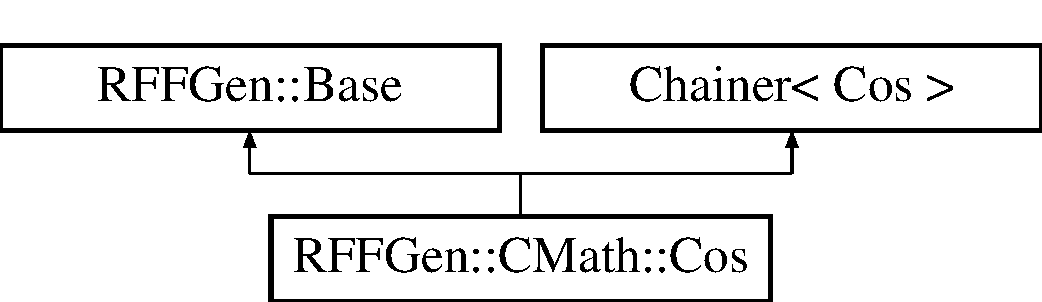
\includegraphics[height=2.000000cm]{structRFFGen_1_1CMath_1_1Cos}
\end{center}
\end{figure}
\subsection*{Public Member Functions}
\begin{DoxyCompactItemize}
\item 
\hyperlink{structRFFGen_1_1CMath_1_1Cos_a950dc0fac1e6a0df91e9beb863af9bee}{Cos} (double x=0.)
\begin{DoxyCompactList}\small\item\em Constructor. \end{DoxyCompactList}\item 
\hypertarget{structRFFGen_1_1CMath_1_1Cos_a2e962b36f84ff276ce63f6bc95d45d04}{void \hyperlink{structRFFGen_1_1CMath_1_1Cos_a2e962b36f84ff276ce63f6bc95d45d04}{update} (const double \&x)}\label{structRFFGen_1_1CMath_1_1Cos_a2e962b36f84ff276ce63f6bc95d45d04}

\begin{DoxyCompactList}\small\item\em Reset point of evaluation. \end{DoxyCompactList}\item 
\hypertarget{structRFFGen_1_1CMath_1_1Cos_a1e5a7d92737ed35ce3c4d3fb5029ba2b}{double \hyperlink{structRFFGen_1_1CMath_1_1Cos_a1e5a7d92737ed35ce3c4d3fb5029ba2b}{d0} () const noexcept}\label{structRFFGen_1_1CMath_1_1Cos_a1e5a7d92737ed35ce3c4d3fb5029ba2b}

\begin{DoxyCompactList}\small\item\em Function value. \end{DoxyCompactList}\item 
\hypertarget{structRFFGen_1_1CMath_1_1Cos_a6813667a131ef0bbf0f8e9acfa7a0575}{{\footnotesize template$<$int  = -\/1$>$ }\\double \hyperlink{structRFFGen_1_1CMath_1_1Cos_a6813667a131ef0bbf0f8e9acfa7a0575}{d1} (double dx=1.) const }\label{structRFFGen_1_1CMath_1_1Cos_a6813667a131ef0bbf0f8e9acfa7a0575}

\begin{DoxyCompactList}\small\item\em First (directional) derivative. \end{DoxyCompactList}\item 
\hypertarget{structRFFGen_1_1CMath_1_1Cos_a748913aa69e699b9d563ed0f44e56384}{{\footnotesize template$<$int  = -\/1, int  = -\/1$>$ }\\double \hyperlink{structRFFGen_1_1CMath_1_1Cos_a748913aa69e699b9d563ed0f44e56384}{d2} (double dx=1., double dy=1.) const }\label{structRFFGen_1_1CMath_1_1Cos_a748913aa69e699b9d563ed0f44e56384}

\begin{DoxyCompactList}\small\item\em Second (directional) derivative. \end{DoxyCompactList}\item 
\hypertarget{structRFFGen_1_1CMath_1_1Cos_a6d003c71b37f3d66d02f55d276b55385}{{\footnotesize template$<$int  = -\/1, int  = -\/1, int  = -\/1$>$ }\\double \hyperlink{structRFFGen_1_1CMath_1_1Cos_a6d003c71b37f3d66d02f55d276b55385}{d3} (double dx=1., double dy=1., double dz=1.) const }\label{structRFFGen_1_1CMath_1_1Cos_a6d003c71b37f3d66d02f55d276b55385}

\begin{DoxyCompactList}\small\item\em Third (directional) derivative. \end{DoxyCompactList}\end{DoxyCompactItemize}


\subsection{Detailed Description}
Cosine function including first three derivatives (based on cos(double) in $<$cmath$>$). 

For scalar functions directional derivatives are less interesting. Incorporating this function as building block for more complex functions requires directional derivatives. These occur during applications of the chain rule.

\begin{DoxySeeAlso}{See Also}
cosine 
\end{DoxySeeAlso}


\subsection{Constructor \& Destructor Documentation}
\hypertarget{structRFFGen_1_1CMath_1_1Cos_a950dc0fac1e6a0df91e9beb863af9bee}{\index{R\-F\-F\-Gen\-::\-C\-Math\-::\-Cos@{R\-F\-F\-Gen\-::\-C\-Math\-::\-Cos}!Cos@{Cos}}
\index{Cos@{Cos}!RFFGen::CMath::Cos@{R\-F\-F\-Gen\-::\-C\-Math\-::\-Cos}}
\subsubsection[{Cos}]{\setlength{\rightskip}{0pt plus 5cm}R\-F\-F\-Gen\-::\-C\-Math\-::\-Cos\-::\-Cos (
\begin{DoxyParamCaption}
\item[{double}]{x = {\ttfamily 0.}}
\end{DoxyParamCaption}
)\hspace{0.3cm}{\ttfamily [inline]}, {\ttfamily [explicit]}}}\label{structRFFGen_1_1CMath_1_1Cos_a950dc0fac1e6a0df91e9beb863af9bee}


Constructor. 


\begin{DoxyParams}{Parameters}
{\em x} & point of evaluation \\
\hline
\end{DoxyParams}


The documentation for this struct was generated from the following file\-:\begin{DoxyCompactItemize}
\item 
R\-F\-F\-Gen/\-C\-Math/cosine.\-hh\end{DoxyCompactItemize}

\hypertarget{structRFFGen_1_1LinearAlgebra_1_1Deviator}{\section{R\-F\-F\-Gen\-:\-:Linear\-Algebra\-:\-:Deviator$<$ Matrix, class $>$ Struct Template Reference}
\label{structRFFGen_1_1LinearAlgebra_1_1Deviator}\index{R\-F\-F\-Gen\-::\-Linear\-Algebra\-::\-Deviator$<$ Matrix, class $>$@{R\-F\-F\-Gen\-::\-Linear\-Algebra\-::\-Deviator$<$ Matrix, class $>$}}
}


Deviator of a matrix $ A\in\mathbb{R}^{n,n} $, i.\-e. $ A - \frac{\mathrm{tr}(A)}{n}I $.  




{\ttfamily \#include $<$deviator.\-hh$>$}

Inheritance diagram for R\-F\-F\-Gen\-:\-:Linear\-Algebra\-:\-:Deviator$<$ Matrix, class $>$\-:\begin{figure}[H]
\begin{center}
\leavevmode
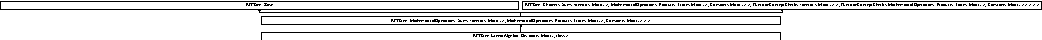
\includegraphics[height=0.555556cm]{structRFFGen_1_1LinearAlgebra_1_1Deviator}
\end{center}
\end{figure}
\subsection*{Public Member Functions}
\begin{DoxyCompactItemize}
\item 
\hyperlink{structRFFGen_1_1LinearAlgebra_1_1Deviator_a38235925f7702700d6adcd1265b62b31}{Deviator} (const Matrix \&A)
\begin{DoxyCompactList}\small\item\em Constructor. \end{DoxyCompactList}\end{DoxyCompactItemize}


\subsection{Detailed Description}
\subsubsection*{template$<$class Matrix, class = Concepts\-::\-Symmetric\-Matrix\-Concept\-Check$<$\-Matrix$>$$>$struct R\-F\-F\-Gen\-::\-Linear\-Algebra\-::\-Deviator$<$ Matrix, class $>$}

Deviator of a matrix $ A\in\mathbb{R}^{n,n} $, i.\-e. $ A - \frac{\mathrm{tr}(A)}{n}I $. 

\subsection{Constructor \& Destructor Documentation}
\hypertarget{structRFFGen_1_1LinearAlgebra_1_1Deviator_a38235925f7702700d6adcd1265b62b31}{\index{R\-F\-F\-Gen\-::\-Linear\-Algebra\-::\-Deviator@{R\-F\-F\-Gen\-::\-Linear\-Algebra\-::\-Deviator}!Deviator@{Deviator}}
\index{Deviator@{Deviator}!RFFGen::LinearAlgebra::Deviator@{R\-F\-F\-Gen\-::\-Linear\-Algebra\-::\-Deviator}}
\subsubsection[{Deviator}]{\setlength{\rightskip}{0pt plus 5cm}template$<$class Matrix , class  = Concepts\-::\-Symmetric\-Matrix\-Concept\-Check$<$\-Matrix$>$$>$ {\bf R\-F\-F\-Gen\-::\-Linear\-Algebra\-::\-Deviator}$<$ Matrix, class $>$\-::{\bf Deviator} (
\begin{DoxyParamCaption}
\item[{const Matrix \&}]{A}
\end{DoxyParamCaption}
)\hspace{0.3cm}{\ttfamily [inline]}, {\ttfamily [explicit]}}}\label{structRFFGen_1_1LinearAlgebra_1_1Deviator_a38235925f7702700d6adcd1265b62b31}


Constructor. 


\begin{DoxyParams}{Parameters}
{\em A} & matrix for which the deviator is computed \\
\hline
\end{DoxyParams}


The documentation for this struct was generated from the following file\-:\begin{DoxyCompactItemize}
\item 
R\-F\-F\-Gen/\-Linear\-Algebra/deviator.\-hh\end{DoxyCompactItemize}

\hypertarget{classRFFGen_1_1LinearAlgebra_1_1DynamicSizeDeterminant}{\section{R\-F\-F\-Gen\-:\-:Linear\-Algebra\-:\-:Dynamic\-Size\-Determinant$<$ Matrix $>$ Class Template Reference}
\label{classRFFGen_1_1LinearAlgebra_1_1DynamicSizeDeterminant}\index{R\-F\-F\-Gen\-::\-Linear\-Algebra\-::\-Dynamic\-Size\-Determinant$<$ Matrix $>$@{R\-F\-F\-Gen\-::\-Linear\-Algebra\-::\-Dynamic\-Size\-Determinant$<$ Matrix $>$}}
}


Determinant of dynamic size matrix with first three derivatives.  




{\ttfamily \#include $<$determinant.\-hh$>$}

Inheritance diagram for R\-F\-F\-Gen\-:\-:Linear\-Algebra\-:\-:Dynamic\-Size\-Determinant$<$ Matrix $>$\-:\begin{figure}[H]
\begin{center}
\leavevmode
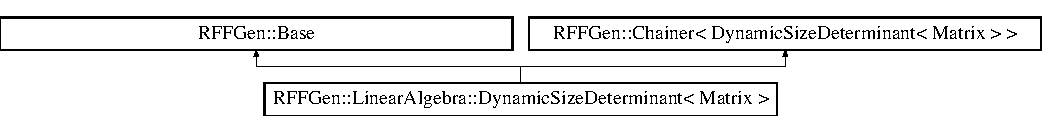
\includegraphics[height=1.559888cm]{classRFFGen_1_1LinearAlgebra_1_1DynamicSizeDeterminant}
\end{center}
\end{figure}
\subsection*{Public Member Functions}
\begin{DoxyCompactItemize}
\item 
\hypertarget{classRFFGen_1_1LinearAlgebra_1_1DynamicSizeDeterminant_a78f820129f3067e04db304b0e3da0f24}{\hyperlink{classRFFGen_1_1LinearAlgebra_1_1DynamicSizeDeterminant_a78f820129f3067e04db304b0e3da0f24}{Dynamic\-Size\-Determinant} (Matrix const \&A)}\label{classRFFGen_1_1LinearAlgebra_1_1DynamicSizeDeterminant_a78f820129f3067e04db304b0e3da0f24}

\begin{DoxyCompactList}\small\item\em Constructor. \end{DoxyCompactList}\item 
\hypertarget{classRFFGen_1_1LinearAlgebra_1_1DynamicSizeDeterminant_ae5f2f4faf564a53f8861783a646f122a}{void \hyperlink{classRFFGen_1_1LinearAlgebra_1_1DynamicSizeDeterminant_ae5f2f4faf564a53f8861783a646f122a}{update} (Matrix const \&A)}\label{classRFFGen_1_1LinearAlgebra_1_1DynamicSizeDeterminant_ae5f2f4faf564a53f8861783a646f122a}

\begin{DoxyCompactList}\small\item\em Reset point of evaluation. \end{DoxyCompactList}\item 
\hypertarget{classRFFGen_1_1LinearAlgebra_1_1DynamicSizeDeterminant_a52543a48ac719e9a3e7df404215ce3ae}{auto \hyperlink{classRFFGen_1_1LinearAlgebra_1_1DynamicSizeDeterminant_a52543a48ac719e9a3e7df404215ce3ae}{d0} () const }\label{classRFFGen_1_1LinearAlgebra_1_1DynamicSizeDeterminant_a52543a48ac719e9a3e7df404215ce3ae}

\begin{DoxyCompactList}\small\item\em Function value. \end{DoxyCompactList}\item 
\hypertarget{classRFFGen_1_1LinearAlgebra_1_1DynamicSizeDeterminant_a65bb49aec31db082d83401f53e0f34b6}{{\footnotesize template$<$int id$>$ }\\auto \hyperlink{classRFFGen_1_1LinearAlgebra_1_1DynamicSizeDeterminant_a65bb49aec31db082d83401f53e0f34b6}{d1} (Matrix const \&d\-A1) const }\label{classRFFGen_1_1LinearAlgebra_1_1DynamicSizeDeterminant_a65bb49aec31db082d83401f53e0f34b6}

\begin{DoxyCompactList}\small\item\em First (directional) derivative. \end{DoxyCompactList}\item 
\hypertarget{classRFFGen_1_1LinearAlgebra_1_1DynamicSizeDeterminant_a8c944d4c6dcc714b265661b6e0c24437}{{\footnotesize template$<$int idx, int idy$>$ }\\auto \hyperlink{classRFFGen_1_1LinearAlgebra_1_1DynamicSizeDeterminant_a8c944d4c6dcc714b265661b6e0c24437}{d2} (Matrix const \&d\-A1, Matrix const \&d\-A2) const }\label{classRFFGen_1_1LinearAlgebra_1_1DynamicSizeDeterminant_a8c944d4c6dcc714b265661b6e0c24437}

\begin{DoxyCompactList}\small\item\em Second (directional) derivative. \end{DoxyCompactList}\item 
\hypertarget{classRFFGen_1_1LinearAlgebra_1_1DynamicSizeDeterminant_a9de4bdf8885f6d5a0449b36d2ff2ab70}{{\footnotesize template$<$int idx, int idy, int idz$>$ }\\auto \hyperlink{classRFFGen_1_1LinearAlgebra_1_1DynamicSizeDeterminant_a9de4bdf8885f6d5a0449b36d2ff2ab70}{d3} (Matrix const \&d\-A1, Matrix const \&d\-A2, Matrix const \&d\-A3) const }\label{classRFFGen_1_1LinearAlgebra_1_1DynamicSizeDeterminant_a9de4bdf8885f6d5a0449b36d2ff2ab70}

\begin{DoxyCompactList}\small\item\em Third (directional) derivative. \end{DoxyCompactList}\end{DoxyCompactItemize}


\subsection{Detailed Description}
\subsubsection*{template$<$class Matrix$>$class R\-F\-F\-Gen\-::\-Linear\-Algebra\-::\-Dynamic\-Size\-Determinant$<$ Matrix $>$}

Determinant of dynamic size matrix with first three derivatives. 

The documentation for this class was generated from the following file\-:\begin{DoxyCompactItemize}
\item 
R\-F\-F\-Gen/\-Linear\-Algebra/determinant.\-hh\end{DoxyCompactItemize}

\hypertarget{structRFFGen_1_1LinearAlgebra_1_1DynamicSizeTrace}{\section{R\-F\-F\-Gen\-:\-:Linear\-Algebra\-:\-:Dynamic\-Size\-Trace$<$ Matrix $>$ Struct Template Reference}
\label{structRFFGen_1_1LinearAlgebra_1_1DynamicSizeTrace}\index{R\-F\-F\-Gen\-::\-Linear\-Algebra\-::\-Dynamic\-Size\-Trace$<$ Matrix $>$@{R\-F\-F\-Gen\-::\-Linear\-Algebra\-::\-Dynamic\-Size\-Trace$<$ Matrix $>$}}
}


Trace of a matrix, i.\-e. sum of diagonal elements.  




{\ttfamily \#include $<$trace.\-hh$>$}

Inheritance diagram for R\-F\-F\-Gen\-:\-:Linear\-Algebra\-:\-:Dynamic\-Size\-Trace$<$ Matrix $>$\-:\begin{figure}[H]
\begin{center}
\leavevmode
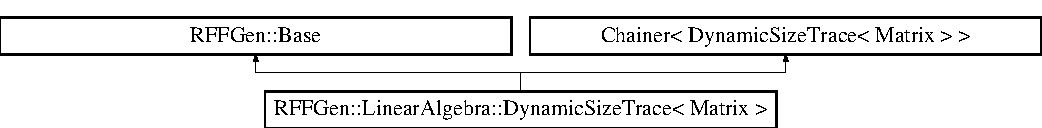
\includegraphics[height=1.723077cm]{structRFFGen_1_1LinearAlgebra_1_1DynamicSizeTrace}
\end{center}
\end{figure}
\subsection*{Public Member Functions}
\begin{DoxyCompactItemize}
\item 
\hypertarget{structRFFGen_1_1LinearAlgebra_1_1DynamicSizeTrace_aef3f5b019aaf94d246487329a2744520}{\hyperlink{structRFFGen_1_1LinearAlgebra_1_1DynamicSizeTrace_aef3f5b019aaf94d246487329a2744520}{Dynamic\-Size\-Trace} ()=default}\label{structRFFGen_1_1LinearAlgebra_1_1DynamicSizeTrace_aef3f5b019aaf94d246487329a2744520}

\begin{DoxyCompactList}\small\item\em Default constructor. \end{DoxyCompactList}\item 
\hyperlink{structRFFGen_1_1LinearAlgebra_1_1DynamicSizeTrace_a0bf007bfd0ab5add26f3033fd4ac54f6}{Dynamic\-Size\-Trace} (const Matrix \&A)
\begin{DoxyCompactList}\small\item\em Constructor. \end{DoxyCompactList}\item 
\hypertarget{structRFFGen_1_1LinearAlgebra_1_1DynamicSizeTrace_a3bebec000fd519643df2d2e0dd2d18ab}{void \hyperlink{structRFFGen_1_1LinearAlgebra_1_1DynamicSizeTrace_a3bebec000fd519643df2d2e0dd2d18ab}{update} (const Matrix \&A)}\label{structRFFGen_1_1LinearAlgebra_1_1DynamicSizeTrace_a3bebec000fd519643df2d2e0dd2d18ab}

\begin{DoxyCompactList}\small\item\em Reset point of evaluation. \end{DoxyCompactList}\item 
\hypertarget{structRFFGen_1_1LinearAlgebra_1_1DynamicSizeTrace_ab6a92df0916c49de8ca6ccfb4c7da0ef}{const auto \& \hyperlink{structRFFGen_1_1LinearAlgebra_1_1DynamicSizeTrace_ab6a92df0916c49de8ca6ccfb4c7da0ef}{operator()} () const noexcept}\label{structRFFGen_1_1LinearAlgebra_1_1DynamicSizeTrace_ab6a92df0916c49de8ca6ccfb4c7da0ef}

\begin{DoxyCompactList}\small\item\em Function value. Convenient access to d0. \end{DoxyCompactList}\item 
\hypertarget{structRFFGen_1_1LinearAlgebra_1_1DynamicSizeTrace_ac091a5832c724173d7bb4477b067cfe1}{const auto \& \hyperlink{structRFFGen_1_1LinearAlgebra_1_1DynamicSizeTrace_ac091a5832c724173d7bb4477b067cfe1}{operator()} (const Matrix \&A) const }\label{structRFFGen_1_1LinearAlgebra_1_1DynamicSizeTrace_ac091a5832c724173d7bb4477b067cfe1}

\begin{DoxyCompactList}\small\item\em Function value. Convenient access to d0 with prior call to update(\-A). \end{DoxyCompactList}\item 
\hypertarget{structRFFGen_1_1LinearAlgebra_1_1DynamicSizeTrace_aaa657dd967d423cd15cc268033f68d36}{const auto \& \hyperlink{structRFFGen_1_1LinearAlgebra_1_1DynamicSizeTrace_aaa657dd967d423cd15cc268033f68d36}{d0} () const noexcept}\label{structRFFGen_1_1LinearAlgebra_1_1DynamicSizeTrace_aaa657dd967d423cd15cc268033f68d36}

\begin{DoxyCompactList}\small\item\em Function value. \end{DoxyCompactList}\item 
\hypertarget{structRFFGen_1_1LinearAlgebra_1_1DynamicSizeTrace_a1357c1190e2ce7e26cd67d178c226458}{{\footnotesize template$<$int $>$ }\\auto \hyperlink{structRFFGen_1_1LinearAlgebra_1_1DynamicSizeTrace_a1357c1190e2ce7e26cd67d178c226458}{d1} (const Matrix \&d\-A) const }\label{structRFFGen_1_1LinearAlgebra_1_1DynamicSizeTrace_a1357c1190e2ce7e26cd67d178c226458}

\begin{DoxyCompactList}\small\item\em First directional derivative. \end{DoxyCompactList}\end{DoxyCompactItemize}


\subsection{Detailed Description}
\subsubsection*{template$<$class Matrix$>$struct R\-F\-F\-Gen\-::\-Linear\-Algebra\-::\-Dynamic\-Size\-Trace$<$ Matrix $>$}

Trace of a matrix, i.\-e. sum of diagonal elements. 

\subsection{Constructor \& Destructor Documentation}
\hypertarget{structRFFGen_1_1LinearAlgebra_1_1DynamicSizeTrace_a0bf007bfd0ab5add26f3033fd4ac54f6}{\index{R\-F\-F\-Gen\-::\-Linear\-Algebra\-::\-Dynamic\-Size\-Trace@{R\-F\-F\-Gen\-::\-Linear\-Algebra\-::\-Dynamic\-Size\-Trace}!Dynamic\-Size\-Trace@{Dynamic\-Size\-Trace}}
\index{Dynamic\-Size\-Trace@{Dynamic\-Size\-Trace}!RFFGen::LinearAlgebra::DynamicSizeTrace@{R\-F\-F\-Gen\-::\-Linear\-Algebra\-::\-Dynamic\-Size\-Trace}}
\subsubsection[{Dynamic\-Size\-Trace}]{\setlength{\rightskip}{0pt plus 5cm}template$<$class Matrix $>$ {\bf R\-F\-F\-Gen\-::\-Linear\-Algebra\-::\-Dynamic\-Size\-Trace}$<$ Matrix $>$\-::{\bf Dynamic\-Size\-Trace} (
\begin{DoxyParamCaption}
\item[{const Matrix \&}]{A}
\end{DoxyParamCaption}
)\hspace{0.3cm}{\ttfamily [inline]}, {\ttfamily [explicit]}}}\label{structRFFGen_1_1LinearAlgebra_1_1DynamicSizeTrace_a0bf007bfd0ab5add26f3033fd4ac54f6}


Constructor. 


\begin{DoxyParams}{Parameters}
{\em A} & point of evaluation. \\
\hline
\end{DoxyParams}


The documentation for this struct was generated from the following file\-:\begin{DoxyCompactItemize}
\item 
R\-F\-F\-Gen/\-Linear\-Algebra/trace.\-hh\end{DoxyCompactItemize}

\hypertarget{structRFFGen_1_1CMath_1_1Exp}{\section{R\-F\-F\-Gen\-:\-:C\-Math\-:\-:Exp Struct Reference}
\label{structRFFGen_1_1CMath_1_1Exp}\index{R\-F\-F\-Gen\-::\-C\-Math\-::\-Exp@{R\-F\-F\-Gen\-::\-C\-Math\-::\-Exp}}
}


Exponential function including first three derivatives.  




{\ttfamily \#include $<$exp.\-hh$>$}

Inheritance diagram for R\-F\-F\-Gen\-:\-:C\-Math\-:\-:Exp\-:\begin{figure}[H]
\begin{center}
\leavevmode
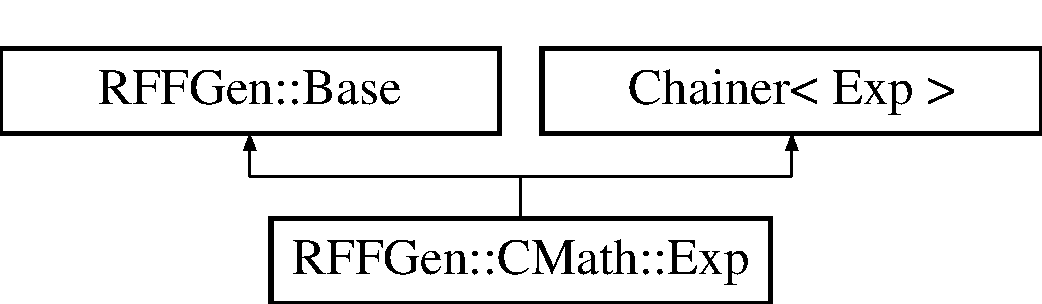
\includegraphics[height=2.000000cm]{structRFFGen_1_1CMath_1_1Exp}
\end{center}
\end{figure}
\subsection*{Public Member Functions}
\begin{DoxyCompactItemize}
\item 
\hyperlink{structRFFGen_1_1CMath_1_1Exp_ac87aaf4564d1e254229f8b8d95798fb6}{Exp} (double x=0.)
\begin{DoxyCompactList}\small\item\em Constructor. \end{DoxyCompactList}\item 
\hypertarget{structRFFGen_1_1CMath_1_1Exp_a7d6b94d4525a3b46a43d80492df7b2c6}{void \hyperlink{structRFFGen_1_1CMath_1_1Exp_a7d6b94d4525a3b46a43d80492df7b2c6}{update} (double x)}\label{structRFFGen_1_1CMath_1_1Exp_a7d6b94d4525a3b46a43d80492df7b2c6}

\begin{DoxyCompactList}\small\item\em Reset point of evaluation. \end{DoxyCompactList}\item 
\hypertarget{structRFFGen_1_1CMath_1_1Exp_ae39b05b64b21becd4df10d485deaf327}{double \hyperlink{structRFFGen_1_1CMath_1_1Exp_ae39b05b64b21becd4df10d485deaf327}{d0} () const noexcept}\label{structRFFGen_1_1CMath_1_1Exp_ae39b05b64b21becd4df10d485deaf327}

\begin{DoxyCompactList}\small\item\em Function value. \end{DoxyCompactList}\item 
\hypertarget{structRFFGen_1_1CMath_1_1Exp_a719d3d0d1c4eb2f51a784c9257769ef3}{{\footnotesize template$<$int  = -\/1$>$ }\\double \hyperlink{structRFFGen_1_1CMath_1_1Exp_a719d3d0d1c4eb2f51a784c9257769ef3}{d1} (double dx=1.) const }\label{structRFFGen_1_1CMath_1_1Exp_a719d3d0d1c4eb2f51a784c9257769ef3}

\begin{DoxyCompactList}\small\item\em First (directional) derivative. \end{DoxyCompactList}\item 
\hypertarget{structRFFGen_1_1CMath_1_1Exp_a2d60b1531ae4346ed9c41d340bdee0c0}{{\footnotesize template$<$int  = -\/1, int  = -\/1$>$ }\\double \hyperlink{structRFFGen_1_1CMath_1_1Exp_a2d60b1531ae4346ed9c41d340bdee0c0}{d2} (double dx=1., double dy=1.) const }\label{structRFFGen_1_1CMath_1_1Exp_a2d60b1531ae4346ed9c41d340bdee0c0}

\begin{DoxyCompactList}\small\item\em Second (directinal) derivative. \end{DoxyCompactList}\item 
\hypertarget{structRFFGen_1_1CMath_1_1Exp_a7dd8dd4b19a3318fd7431d42c8665a5d}{{\footnotesize template$<$int  = -\/1, int  = -\/1, int  = -\/1$>$ }\\double \hyperlink{structRFFGen_1_1CMath_1_1Exp_a7dd8dd4b19a3318fd7431d42c8665a5d}{d3} (double dx=1., double dy=1., double dz=1.) const }\label{structRFFGen_1_1CMath_1_1Exp_a7dd8dd4b19a3318fd7431d42c8665a5d}

\begin{DoxyCompactList}\small\item\em Third (directional) derivative. \end{DoxyCompactList}\end{DoxyCompactItemize}


\subsection{Detailed Description}
Exponential function including first three derivatives. 

For scalar functions directional derivatives are less interesting. Incorporating this function as building block for more complex functions requires directional derivatives. These occur during applications of the chain rule. 

\subsection{Constructor \& Destructor Documentation}
\hypertarget{structRFFGen_1_1CMath_1_1Exp_ac87aaf4564d1e254229f8b8d95798fb6}{\index{R\-F\-F\-Gen\-::\-C\-Math\-::\-Exp@{R\-F\-F\-Gen\-::\-C\-Math\-::\-Exp}!Exp@{Exp}}
\index{Exp@{Exp}!RFFGen::CMath::Exp@{R\-F\-F\-Gen\-::\-C\-Math\-::\-Exp}}
\subsubsection[{Exp}]{\setlength{\rightskip}{0pt plus 5cm}R\-F\-F\-Gen\-::\-C\-Math\-::\-Exp\-::\-Exp (
\begin{DoxyParamCaption}
\item[{double}]{x = {\ttfamily 0.}}
\end{DoxyParamCaption}
)\hspace{0.3cm}{\ttfamily [inline]}, {\ttfamily [explicit]}}}\label{structRFFGen_1_1CMath_1_1Exp_ac87aaf4564d1e254229f8b8d95798fb6}


Constructor. 


\begin{DoxyParams}{Parameters}
{\em x} & point of evaluation \\
\hline
\end{DoxyParams}


The documentation for this struct was generated from the following file\-:\begin{DoxyCompactItemize}
\item 
R\-F\-F\-Gen/\-C\-Math/exp.\-hh\end{DoxyCompactItemize}

\hypertarget{structRFFGen_1_1CMath_1_1Exp2}{\section{R\-F\-F\-Gen\-:\-:C\-Math\-:\-:Exp2 Struct Reference}
\label{structRFFGen_1_1CMath_1_1Exp2}\index{R\-F\-F\-Gen\-::\-C\-Math\-::\-Exp2@{R\-F\-F\-Gen\-::\-C\-Math\-::\-Exp2}}
}


Function $2^x$ including first three derivatives.  




{\ttfamily \#include $<$exp.\-hh$>$}

Inheritance diagram for R\-F\-F\-Gen\-:\-:C\-Math\-:\-:Exp2\-:\begin{figure}[H]
\begin{center}
\leavevmode
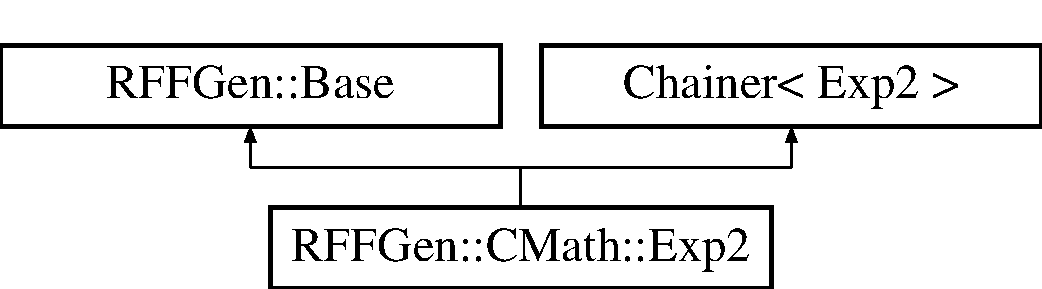
\includegraphics[height=2.000000cm]{structRFFGen_1_1CMath_1_1Exp2}
\end{center}
\end{figure}
\subsection*{Public Member Functions}
\begin{DoxyCompactItemize}
\item 
\hyperlink{structRFFGen_1_1CMath_1_1Exp2_a4df27b5cd85288709f76a87efc4a5a87}{Exp2} (double x=0.)
\begin{DoxyCompactList}\small\item\em Constructor. \end{DoxyCompactList}\item 
\hypertarget{structRFFGen_1_1CMath_1_1Exp2_af856a702894e2b5f444984c4b92882ed}{void \hyperlink{structRFFGen_1_1CMath_1_1Exp2_af856a702894e2b5f444984c4b92882ed}{update} (double x)}\label{structRFFGen_1_1CMath_1_1Exp2_af856a702894e2b5f444984c4b92882ed}

\begin{DoxyCompactList}\small\item\em Reset point of evaluation. \end{DoxyCompactList}\item 
\hypertarget{structRFFGen_1_1CMath_1_1Exp2_ad01d7bed26c83e69766cb187a9359b71}{double \hyperlink{structRFFGen_1_1CMath_1_1Exp2_ad01d7bed26c83e69766cb187a9359b71}{d0} () const noexcept}\label{structRFFGen_1_1CMath_1_1Exp2_ad01d7bed26c83e69766cb187a9359b71}

\begin{DoxyCompactList}\small\item\em Function value. \end{DoxyCompactList}\item 
\hypertarget{structRFFGen_1_1CMath_1_1Exp2_ae9cc83857d461fda21677645ef3cbe3e}{{\footnotesize template$<$int  = -\/1$>$ }\\double \hyperlink{structRFFGen_1_1CMath_1_1Exp2_ae9cc83857d461fda21677645ef3cbe3e}{d1} (double dx=1.) const }\label{structRFFGen_1_1CMath_1_1Exp2_ae9cc83857d461fda21677645ef3cbe3e}

\begin{DoxyCompactList}\small\item\em First (directional) derivative. \end{DoxyCompactList}\item 
\hypertarget{structRFFGen_1_1CMath_1_1Exp2_a39908c16315397ea219d219f1112bdfb}{{\footnotesize template$<$int  = -\/1, int  = -\/1$>$ }\\double \hyperlink{structRFFGen_1_1CMath_1_1Exp2_a39908c16315397ea219d219f1112bdfb}{d2} (double dx=1., double dy=1.) const }\label{structRFFGen_1_1CMath_1_1Exp2_a39908c16315397ea219d219f1112bdfb}

\begin{DoxyCompactList}\small\item\em Second (directinal) derivative. \end{DoxyCompactList}\item 
\hypertarget{structRFFGen_1_1CMath_1_1Exp2_a536a6a91d01b3d6eb713e6908dd374be}{{\footnotesize template$<$int  = -\/1, int  = -\/1, int  = -\/1$>$ }\\double \hyperlink{structRFFGen_1_1CMath_1_1Exp2_a536a6a91d01b3d6eb713e6908dd374be}{d3} (double dx=1., double dy=1., double dz=1.) const }\label{structRFFGen_1_1CMath_1_1Exp2_a536a6a91d01b3d6eb713e6908dd374be}

\begin{DoxyCompactList}\small\item\em Third (directional) derivative. \end{DoxyCompactList}\end{DoxyCompactItemize}


\subsection{Detailed Description}
Function $2^x$ including first three derivatives. 

For scalar functions directional derivatives are less interesting. Incorporating this function as building block for more complex functions requires directional derivatives. These occur during applications of the chain rule. 

\subsection{Constructor \& Destructor Documentation}
\hypertarget{structRFFGen_1_1CMath_1_1Exp2_a4df27b5cd85288709f76a87efc4a5a87}{\index{R\-F\-F\-Gen\-::\-C\-Math\-::\-Exp2@{R\-F\-F\-Gen\-::\-C\-Math\-::\-Exp2}!Exp2@{Exp2}}
\index{Exp2@{Exp2}!RFFGen::CMath::Exp2@{R\-F\-F\-Gen\-::\-C\-Math\-::\-Exp2}}
\subsubsection[{Exp2}]{\setlength{\rightskip}{0pt plus 5cm}R\-F\-F\-Gen\-::\-C\-Math\-::\-Exp2\-::\-Exp2 (
\begin{DoxyParamCaption}
\item[{double}]{x = {\ttfamily 0.}}
\end{DoxyParamCaption}
)\hspace{0.3cm}{\ttfamily [inline]}, {\ttfamily [explicit]}}}\label{structRFFGen_1_1CMath_1_1Exp2_a4df27b5cd85288709f76a87efc4a5a87}


Constructor. 


\begin{DoxyParams}{Parameters}
{\em x} & point of evaluation \\
\hline
\end{DoxyParams}


The documentation for this struct was generated from the following file\-:\begin{DoxyCompactItemize}
\item 
R\-F\-F\-Gen/\-C\-Math/exp.\-hh\end{DoxyCompactItemize}

\hypertarget{structRFFGen_1_1LinearAlgebra_1_1ExtractDimension}{\section{R\-F\-F\-Gen\-:\-:Linear\-Algebra\-:\-:Extract\-Dimension$<$ Matrix, class $>$ Struct Template Reference}
\label{structRFFGen_1_1LinearAlgebra_1_1ExtractDimension}\index{R\-F\-F\-Gen\-::\-Linear\-Algebra\-::\-Extract\-Dimension$<$ Matrix, class $>$@{R\-F\-F\-Gen\-::\-Linear\-Algebra\-::\-Extract\-Dimension$<$ Matrix, class $>$}}
}


Specialize this for your matrix class. Dimension (number of rows/columns for square matrices) must be provided by a static member variable called value.  




{\ttfamily \#include $<$dimension.\-hh$>$}

Inheritance diagram for R\-F\-F\-Gen\-:\-:Linear\-Algebra\-:\-:Extract\-Dimension$<$ Matrix, class $>$\-:\begin{figure}[H]
\begin{center}
\leavevmode
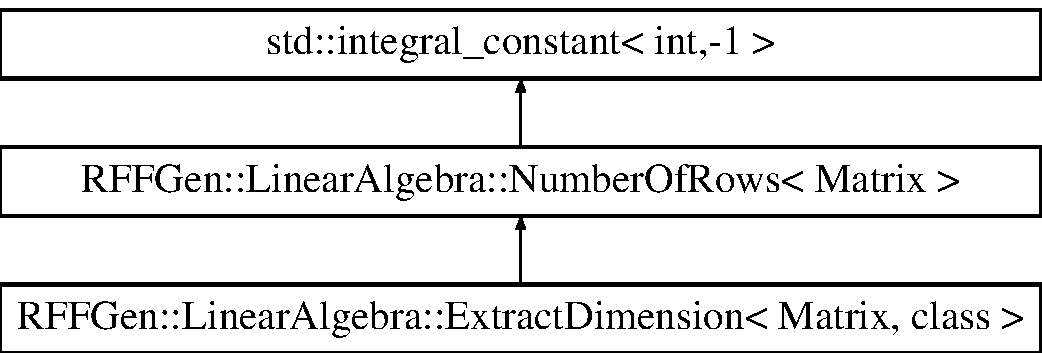
\includegraphics[height=3.000000cm]{structRFFGen_1_1LinearAlgebra_1_1ExtractDimension}
\end{center}
\end{figure}


\subsection{Detailed Description}
\subsubsection*{template$<$class Matrix, class = Concepts\-::\-Symmetric\-Matrix\-Concept\-Check$<$\-Matrix$>$$>$struct R\-F\-F\-Gen\-::\-Linear\-Algebra\-::\-Extract\-Dimension$<$ Matrix, class $>$}

Specialize this for your matrix class. Dimension (number of rows/columns for square matrices) must be provided by a static member variable called value. 

The documentation for this struct was generated from the following file\-:\begin{DoxyCompactItemize}
\item 
R\-F\-F\-Gen/\-Linear\-Algebra/dimension.\-hh\end{DoxyCompactItemize}

\hypertarget{structRFFGen_1_1LinearAlgebra_1_1FirstModifiedMixedInvariant}{\section{R\-F\-F\-Gen\-:\-:Linear\-Algebra\-:\-:First\-Modified\-Mixed\-Invariant$<$ Matrix, class $>$ Struct Template Reference}
\label{structRFFGen_1_1LinearAlgebra_1_1FirstModifiedMixedInvariant}\index{R\-F\-F\-Gen\-::\-Linear\-Algebra\-::\-First\-Modified\-Mixed\-Invariant$<$ Matrix, class $>$@{R\-F\-F\-Gen\-::\-Linear\-Algebra\-::\-First\-Modified\-Mixed\-Invariant$<$ Matrix, class $>$}}
}


First modified mixed invariant $\bar\iota_4=\iota_4\iota_3^{-1/3}$.  




{\ttfamily \#include $<$modified\-Mixed\-Invariants.\-hh$>$}

Inheritance diagram for R\-F\-F\-Gen\-:\-:Linear\-Algebra\-:\-:First\-Modified\-Mixed\-Invariant$<$ Matrix, class $>$\-:\begin{figure}[H]
\begin{center}
\leavevmode
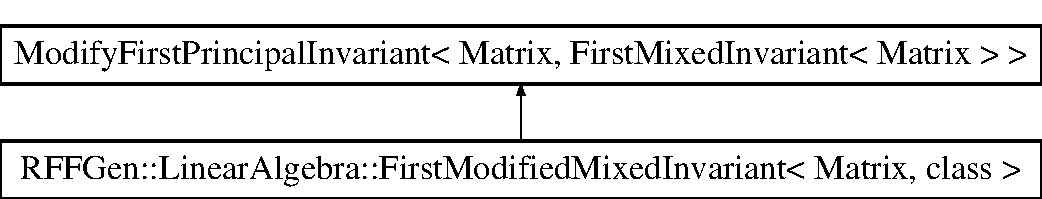
\includegraphics[height=2.000000cm]{structRFFGen_1_1LinearAlgebra_1_1FirstModifiedMixedInvariant}
\end{center}
\end{figure}
\subsection*{Public Member Functions}
\begin{DoxyCompactItemize}
\item 
\hypertarget{structRFFGen_1_1LinearAlgebra_1_1FirstModifiedMixedInvariant_a81fca73557d2c6bc0cd773bd9431cb64}{\hyperlink{structRFFGen_1_1LinearAlgebra_1_1FirstModifiedMixedInvariant_a81fca73557d2c6bc0cd773bd9431cb64}{First\-Modified\-Mixed\-Invariant} ()=default}\label{structRFFGen_1_1LinearAlgebra_1_1FirstModifiedMixedInvariant_a81fca73557d2c6bc0cd773bd9431cb64}

\begin{DoxyCompactList}\small\item\em Default constructor. \end{DoxyCompactList}\item 
\hyperlink{structRFFGen_1_1LinearAlgebra_1_1FirstModifiedMixedInvariant_a8b88a33160220e42121a05876a27d480}{First\-Modified\-Mixed\-Invariant} (const Matrix \&A, const \hyperlink{structRFFGen_1_1Constant}{Constant}$<$ Matrix $>$ \&M)
\begin{DoxyCompactList}\small\item\em Constructor. \end{DoxyCompactList}\item 
\hyperlink{structRFFGen_1_1LinearAlgebra_1_1FirstModifiedMixedInvariant_acb5d04a5302a1b2e5b1dc1fafbc8a63f}{First\-Modified\-Mixed\-Invariant} (const std\-::tuple$<$ Matrix, \hyperlink{structRFFGen_1_1Constant}{Constant}$<$ Matrix $>$ $>$ \&t)
\begin{DoxyCompactList}\small\item\em Constructor from std\-::tuple. \end{DoxyCompactList}\end{DoxyCompactItemize}


\subsection{Detailed Description}
\subsubsection*{template$<$class Matrix, class = Concepts\-::\-Symmetric\-Matrix\-Concept\-Check$<$\-Matrix$>$$>$struct R\-F\-F\-Gen\-::\-Linear\-Algebra\-::\-First\-Modified\-Mixed\-Invariant$<$ Matrix, class $>$}

First modified mixed invariant $\bar\iota_4=\iota_4\iota_3^{-1/3}$. 

\subsection{Constructor \& Destructor Documentation}
\hypertarget{structRFFGen_1_1LinearAlgebra_1_1FirstModifiedMixedInvariant_a8b88a33160220e42121a05876a27d480}{\index{R\-F\-F\-Gen\-::\-Linear\-Algebra\-::\-First\-Modified\-Mixed\-Invariant@{R\-F\-F\-Gen\-::\-Linear\-Algebra\-::\-First\-Modified\-Mixed\-Invariant}!First\-Modified\-Mixed\-Invariant@{First\-Modified\-Mixed\-Invariant}}
\index{First\-Modified\-Mixed\-Invariant@{First\-Modified\-Mixed\-Invariant}!RFFGen::LinearAlgebra::FirstModifiedMixedInvariant@{R\-F\-F\-Gen\-::\-Linear\-Algebra\-::\-First\-Modified\-Mixed\-Invariant}}
\subsubsection[{First\-Modified\-Mixed\-Invariant}]{\setlength{\rightskip}{0pt plus 5cm}template$<$class Matrix , class  = Concepts\-::\-Symmetric\-Matrix\-Concept\-Check$<$\-Matrix$>$$>$ {\bf R\-F\-F\-Gen\-::\-Linear\-Algebra\-::\-First\-Modified\-Mixed\-Invariant}$<$ Matrix, class $>$\-::{\bf First\-Modified\-Mixed\-Invariant} (
\begin{DoxyParamCaption}
\item[{const Matrix \&}]{A, }
\item[{const {\bf Constant}$<$ Matrix $>$ \&}]{M}
\end{DoxyParamCaption}
)\hspace{0.3cm}{\ttfamily [inline]}}}\label{structRFFGen_1_1LinearAlgebra_1_1FirstModifiedMixedInvariant_a8b88a33160220e42121a05876a27d480}


Constructor. 


\begin{DoxyParams}{Parameters}
{\em A} & matrix to compute first modified mixed invariant from. \\
\hline
{\em M} & structural tensor incorporating anisotropic information. \\
\hline
\end{DoxyParams}
\hypertarget{structRFFGen_1_1LinearAlgebra_1_1FirstModifiedMixedInvariant_acb5d04a5302a1b2e5b1dc1fafbc8a63f}{\index{R\-F\-F\-Gen\-::\-Linear\-Algebra\-::\-First\-Modified\-Mixed\-Invariant@{R\-F\-F\-Gen\-::\-Linear\-Algebra\-::\-First\-Modified\-Mixed\-Invariant}!First\-Modified\-Mixed\-Invariant@{First\-Modified\-Mixed\-Invariant}}
\index{First\-Modified\-Mixed\-Invariant@{First\-Modified\-Mixed\-Invariant}!RFFGen::LinearAlgebra::FirstModifiedMixedInvariant@{R\-F\-F\-Gen\-::\-Linear\-Algebra\-::\-First\-Modified\-Mixed\-Invariant}}
\subsubsection[{First\-Modified\-Mixed\-Invariant}]{\setlength{\rightskip}{0pt plus 5cm}template$<$class Matrix , class  = Concepts\-::\-Symmetric\-Matrix\-Concept\-Check$<$\-Matrix$>$$>$ {\bf R\-F\-F\-Gen\-::\-Linear\-Algebra\-::\-First\-Modified\-Mixed\-Invariant}$<$ Matrix, class $>$\-::{\bf First\-Modified\-Mixed\-Invariant} (
\begin{DoxyParamCaption}
\item[{const std\-::tuple$<$ Matrix, {\bf Constant}$<$ Matrix $>$ $>$ \&}]{t}
\end{DoxyParamCaption}
)\hspace{0.3cm}{\ttfamily [inline]}}}\label{structRFFGen_1_1LinearAlgebra_1_1FirstModifiedMixedInvariant_acb5d04a5302a1b2e5b1dc1fafbc8a63f}


Constructor from std\-::tuple. 


\begin{DoxyParams}{Parameters}
{\em t} & st\-::get$<$0$>$(t)\-: matrix to compute first modified invariant form, std\-::get$<$1$>$(t)\-: structural tensor \\
\hline
\end{DoxyParams}


The documentation for this struct was generated from the following file\-:\begin{DoxyCompactItemize}
\item 
R\-F\-F\-Gen/\-Linear\-Algebra/modified\-Mixed\-Invariants.\-hh\end{DoxyCompactItemize}

\hypertarget{structRFFGen_1_1LinearAlgebra_1_1FirstModifiedPrincipalInvariant}{\section{R\-F\-F\-Gen\-:\-:Linear\-Algebra\-:\-:First\-Modified\-Principal\-Invariant$<$ Matrix, class $>$ Struct Template Reference}
\label{structRFFGen_1_1LinearAlgebra_1_1FirstModifiedPrincipalInvariant}\index{R\-F\-F\-Gen\-::\-Linear\-Algebra\-::\-First\-Modified\-Principal\-Invariant$<$ Matrix, class $>$@{R\-F\-F\-Gen\-::\-Linear\-Algebra\-::\-First\-Modified\-Principal\-Invariant$<$ Matrix, class $>$}}
}


Isochoric (volume-\/preserving), first modified principal invariant $ \bar\iota_1(A)=\iota_1\iota_3^{-1/3} $, where $\iota_1$ is the first and $\iota_3$ is the third principal invariant.  




{\ttfamily \#include $<$modified\-Principal\-Invariants.\-hh$>$}

Inheritance diagram for R\-F\-F\-Gen\-:\-:Linear\-Algebra\-:\-:First\-Modified\-Principal\-Invariant$<$ Matrix, class $>$\-:\begin{figure}[H]
\begin{center}
\leavevmode
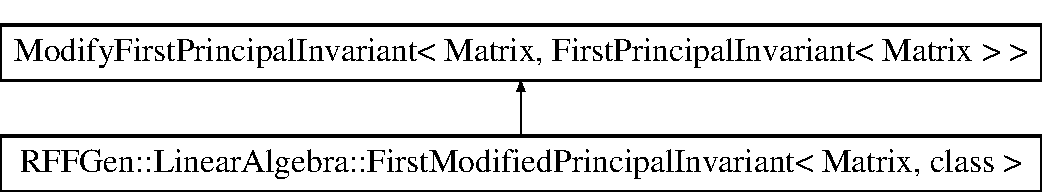
\includegraphics[height=2.000000cm]{structRFFGen_1_1LinearAlgebra_1_1FirstModifiedPrincipalInvariant}
\end{center}
\end{figure}
\subsection*{Public Member Functions}
\begin{DoxyCompactItemize}
\item 
\hypertarget{structRFFGen_1_1LinearAlgebra_1_1FirstModifiedPrincipalInvariant_a9bac4f0c2ec989db534c94378a0b48f3}{\hyperlink{structRFFGen_1_1LinearAlgebra_1_1FirstModifiedPrincipalInvariant_a9bac4f0c2ec989db534c94378a0b48f3}{First\-Modified\-Principal\-Invariant} ()=default}\label{structRFFGen_1_1LinearAlgebra_1_1FirstModifiedPrincipalInvariant_a9bac4f0c2ec989db534c94378a0b48f3}

\begin{DoxyCompactList}\small\item\em Default constructor. \end{DoxyCompactList}\item 
\hyperlink{structRFFGen_1_1LinearAlgebra_1_1FirstModifiedPrincipalInvariant_a241d5c718a2648527fc1dddf1bc9349b}{First\-Modified\-Principal\-Invariant} (const Matrix \&A)
\begin{DoxyCompactList}\small\item\em Constructor. \end{DoxyCompactList}\end{DoxyCompactItemize}


\subsection{Detailed Description}
\subsubsection*{template$<$class Matrix, class = Concepts\-::\-Symmetric\-Matrix\-Concept\-Check$<$\-Matrix$>$$>$struct R\-F\-F\-Gen\-::\-Linear\-Algebra\-::\-First\-Modified\-Principal\-Invariant$<$ Matrix, class $>$}

Isochoric (volume-\/preserving), first modified principal invariant $ \bar\iota_1(A)=\iota_1\iota_3^{-1/3} $, where $\iota_1$ is the first and $\iota_3$ is the third principal invariant. 

\subsection{Constructor \& Destructor Documentation}
\hypertarget{structRFFGen_1_1LinearAlgebra_1_1FirstModifiedPrincipalInvariant_a241d5c718a2648527fc1dddf1bc9349b}{\index{R\-F\-F\-Gen\-::\-Linear\-Algebra\-::\-First\-Modified\-Principal\-Invariant@{R\-F\-F\-Gen\-::\-Linear\-Algebra\-::\-First\-Modified\-Principal\-Invariant}!First\-Modified\-Principal\-Invariant@{First\-Modified\-Principal\-Invariant}}
\index{First\-Modified\-Principal\-Invariant@{First\-Modified\-Principal\-Invariant}!RFFGen::LinearAlgebra::FirstModifiedPrincipalInvariant@{R\-F\-F\-Gen\-::\-Linear\-Algebra\-::\-First\-Modified\-Principal\-Invariant}}
\subsubsection[{First\-Modified\-Principal\-Invariant}]{\setlength{\rightskip}{0pt plus 5cm}template$<$class Matrix , class  = Concepts\-::\-Symmetric\-Matrix\-Concept\-Check$<$\-Matrix$>$$>$ {\bf R\-F\-F\-Gen\-::\-Linear\-Algebra\-::\-First\-Modified\-Principal\-Invariant}$<$ Matrix, class $>$\-::{\bf First\-Modified\-Principal\-Invariant} (
\begin{DoxyParamCaption}
\item[{const Matrix \&}]{A}
\end{DoxyParamCaption}
)\hspace{0.3cm}{\ttfamily [inline]}}}\label{structRFFGen_1_1LinearAlgebra_1_1FirstModifiedPrincipalInvariant_a241d5c718a2648527fc1dddf1bc9349b}


Constructor. 


\begin{DoxyParams}{Parameters}
{\em A} & matrix to compute first modified principal invariant from. \\
\hline
\end{DoxyParams}


The documentation for this struct was generated from the following file\-:\begin{DoxyCompactItemize}
\item 
R\-F\-F\-Gen/\-Linear\-Algebra/modified\-Principal\-Invariants.\-hh\end{DoxyCompactItemize}

\hypertarget{structRFFGen_1_1Concepts_1_1FunctionConcept}{\section{R\-F\-F\-Gen\-:\-:Concepts\-:\-:Function\-Concept Struct Reference}
\label{structRFFGen_1_1Concepts_1_1FunctionConcept}\index{R\-F\-F\-Gen\-::\-Concepts\-::\-Function\-Concept@{R\-F\-F\-Gen\-::\-Concepts\-::\-Function\-Concept}}
}


Minimal requirements for functions.  




{\ttfamily \#include $<$concepts.\-hh$>$}

Inheritance diagram for R\-F\-F\-Gen\-:\-:Concepts\-:\-:Function\-Concept\-:\begin{figure}[H]
\begin{center}
\leavevmode
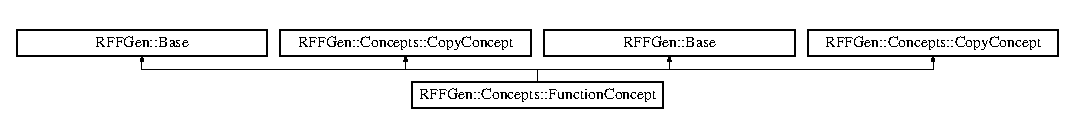
\includegraphics[height=2.000000cm]{structRFFGen_1_1Concepts_1_1FunctionConcept}
\end{center}
\end{figure}
\subsection*{Public Member Functions}
\begin{DoxyCompactItemize}
\item 
\hypertarget{structRFFGen_1_1Concepts_1_1FunctionConcept_a6006207e743a93b96d2d603b8b75bd7c}{unspecified \hyperlink{structRFFGen_1_1Concepts_1_1FunctionConcept_a6006207e743a93b96d2d603b8b75bd7c}{d0} () const }\label{structRFFGen_1_1Concepts_1_1FunctionConcept_a6006207e743a93b96d2d603b8b75bd7c}

\begin{DoxyCompactList}\small\item\em Access to function value. \end{DoxyCompactList}\end{DoxyCompactItemize}


\subsection{Detailed Description}
Minimal requirements for functions. 

The documentation for this struct was generated from the following file\-:\begin{DoxyCompactItemize}
\item 
R\-F\-F\-Gen/\hyperlink{concepts_8hh}{concepts.\-hh}\end{DoxyCompactItemize}

\hypertarget{structRFFGen_1_1Concepts_1_1FunctionConceptCheck}{\section{R\-F\-F\-Gen\-:\-:Concepts\-:\-:Function\-Concept\-Check$<$ F $>$ Struct Template Reference}
\label{structRFFGen_1_1Concepts_1_1FunctionConceptCheck}\index{R\-F\-F\-Gen\-::\-Concepts\-::\-Function\-Concept\-Check$<$ F $>$@{R\-F\-F\-Gen\-::\-Concepts\-::\-Function\-Concept\-Check$<$ F $>$}}
}


Static check if the requirements of \hyperlink{structRFFGen_1_1Concepts_1_1FunctionConcept}{Function\-Concept} are satisfied.  




{\ttfamily \#include $<$concept\-Check.\-hh$>$}

Inheritance diagram for R\-F\-F\-Gen\-:\-:Concepts\-:\-:Function\-Concept\-Check$<$ F $>$\-:\begin{figure}[H]
\begin{center}
\leavevmode
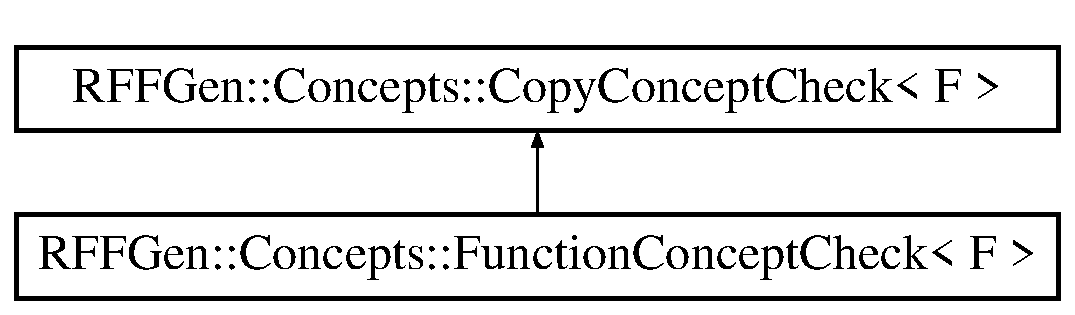
\includegraphics[height=2.000000cm]{structRFFGen_1_1Concepts_1_1FunctionConceptCheck}
\end{center}
\end{figure}


\subsection{Detailed Description}
\subsubsection*{template$<$class F$>$struct R\-F\-F\-Gen\-::\-Concepts\-::\-Function\-Concept\-Check$<$ F $>$}

Static check if the requirements of \hyperlink{structRFFGen_1_1Concepts_1_1FunctionConcept}{Function\-Concept} are satisfied. 

The documentation for this struct was generated from the following file\-:\begin{DoxyCompactItemize}
\item 
R\-F\-F\-Gen/concept\-Check.\-hh\end{DoxyCompactItemize}

\hypertarget{structRFFGen_1_1Identity}{\section{R\-F\-F\-Gen\-:\-:Identity$<$ Arg, class $>$ Struct Template Reference}
\label{structRFFGen_1_1Identity}\index{R\-F\-F\-Gen\-::\-Identity$<$ Arg, class $>$@{R\-F\-F\-Gen\-::\-Identity$<$ Arg, class $>$}}
}


Identity mapping $ f(x)=x $.  




{\ttfamily \#include $<$identity.\-hh$>$}

Inheritance diagram for R\-F\-F\-Gen\-:\-:Identity$<$ Arg, class $>$\-:\begin{figure}[H]
\begin{center}
\leavevmode
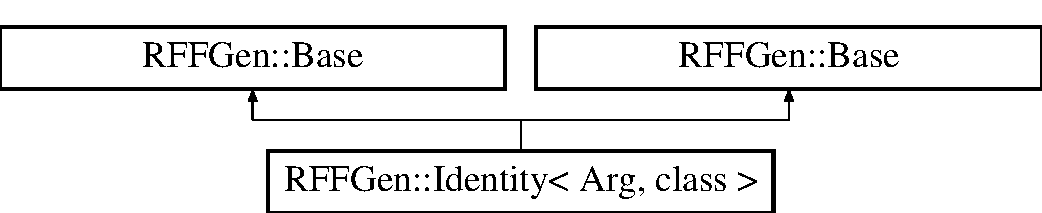
\includegraphics[height=1.525886cm]{structRFFGen_1_1Identity}
\end{center}
\end{figure}
\subsection*{Public Member Functions}
\begin{DoxyCompactItemize}
\item 
\hypertarget{structRFFGen_1_1Identity_a8b78693b14060a66fe32e8a15df1873a}{\hyperlink{structRFFGen_1_1Identity_a8b78693b14060a66fe32e8a15df1873a}{Identity} ()=default}\label{structRFFGen_1_1Identity_a8b78693b14060a66fe32e8a15df1873a}

\begin{DoxyCompactList}\small\item\em Default constructor. \end{DoxyCompactList}\item 
\hyperlink{structRFFGen_1_1Identity_ad1206bbe037c72a77aa90119f228f9e2}{Identity} (const Arg \&x)
\begin{DoxyCompactList}\small\item\em Constructor. \end{DoxyCompactList}\item 
\hypertarget{structRFFGen_1_1Identity_a0ddfb34c7d8f2edb9648dedf046164c8}{void \hyperlink{structRFFGen_1_1Identity_a0ddfb34c7d8f2edb9648dedf046164c8}{update} (const Arg \&x)}\label{structRFFGen_1_1Identity_a0ddfb34c7d8f2edb9648dedf046164c8}

\begin{DoxyCompactList}\small\item\em Reset point of evaluation. \end{DoxyCompactList}\item 
\hypertarget{structRFFGen_1_1Identity_a41c728eda635f547da2a0b697876ca63}{const Arg \& \hyperlink{structRFFGen_1_1Identity_a41c728eda635f547da2a0b697876ca63}{d0} () const noexcept}\label{structRFFGen_1_1Identity_a41c728eda635f547da2a0b697876ca63}

\begin{DoxyCompactList}\small\item\em Function value. \end{DoxyCompactList}\item 
\hypertarget{structRFFGen_1_1Identity_a0a2fba6a1d3326df7de1f329e20dd557}{{\footnotesize template$<$int $>$ }\\const Arg \& \hyperlink{structRFFGen_1_1Identity_a0a2fba6a1d3326df7de1f329e20dd557}{d1} (const Arg \&dx) const noexcept}\label{structRFFGen_1_1Identity_a0a2fba6a1d3326df7de1f329e20dd557}

\begin{DoxyCompactList}\small\item\em First directional derivative. \end{DoxyCompactList}\end{DoxyCompactItemize}


\subsection{Detailed Description}
\subsubsection*{template$<$class Arg, class = Arithmetic\-Concept\-Check$<$\-Arg$>$$>$struct R\-F\-F\-Gen\-::\-Identity$<$ Arg, class $>$}

Identity mapping $ f(x)=x $. 

\subsection{Constructor \& Destructor Documentation}
\hypertarget{structRFFGen_1_1Identity_ad1206bbe037c72a77aa90119f228f9e2}{\index{R\-F\-F\-Gen\-::\-Identity@{R\-F\-F\-Gen\-::\-Identity}!Identity@{Identity}}
\index{Identity@{Identity}!RFFGen::Identity@{R\-F\-F\-Gen\-::\-Identity}}
\subsubsection[{Identity}]{\setlength{\rightskip}{0pt plus 5cm}template$<$class Arg , class  = Arithmetic\-Concept\-Check$<$\-Arg$>$$>$ {\bf R\-F\-F\-Gen\-::\-Identity}$<$ Arg, class $>$\-::{\bf Identity} (
\begin{DoxyParamCaption}
\item[{const Arg \&}]{x}
\end{DoxyParamCaption}
)\hspace{0.3cm}{\ttfamily [inline]}}}\label{structRFFGen_1_1Identity_ad1206bbe037c72a77aa90119f228f9e2}


Constructor. 


\begin{DoxyParams}{Parameters}
{\em x} & point of evaluation. \\
\hline
\end{DoxyParams}


The documentation for this struct was generated from the following file\-:\begin{DoxyCompactItemize}
\item 
R\-F\-F\-Gen/identity.\-hh\end{DoxyCompactItemize}

\hypertarget{structRFFGen_1_1LinearAlgebra_1_1InvariantTraits_3_01Invariant_1_1MIXED_01_4}{\section{R\-F\-F\-Gen\-:\-:Linear\-Algebra\-:\-:Invariant\-Traits$<$ Invariant\-:\-:M\-I\-X\-E\-D $>$ Struct Template Reference}
\label{structRFFGen_1_1LinearAlgebra_1_1InvariantTraits_3_01Invariant_1_1MIXED_01_4}\index{R\-F\-F\-Gen\-::\-Linear\-Algebra\-::\-Invariant\-Traits$<$ Invariant\-::\-M\-I\-X\-E\-D $>$@{R\-F\-F\-Gen\-::\-Linear\-Algebra\-::\-Invariant\-Traits$<$ Invariant\-::\-M\-I\-X\-E\-D $>$}}
}


Traits class for access of (shifted) mixed invariants.  




{\ttfamily \#include $<$invariants.\-hh$>$}

\subsection*{Public Types}
\begin{DoxyCompactItemize}
\item 
\hypertarget{structRFFGen_1_1LinearAlgebra_1_1InvariantTraits_3_01Invariant_1_1MIXED_01_4_a353d608986625e7dc9b6652036e8fd73}{{\footnotesize template$<$class Matrix $>$ }\\using \hyperlink{structRFFGen_1_1LinearAlgebra_1_1InvariantTraits_3_01Invariant_1_1MIXED_01_4_a353d608986625e7dc9b6652036e8fd73}{First\-Invariant} = \hyperlink{group__InvariantGroup_ga9896f1432dd23593f147c31c0be9ccde}{First\-Mixed\-Invariant}$<$ Matrix $>$}\label{structRFFGen_1_1LinearAlgebra_1_1InvariantTraits_3_01Invariant_1_1MIXED_01_4_a353d608986625e7dc9b6652036e8fd73}

\begin{DoxyCompactList}\small\item\em First mixed invariant. \end{DoxyCompactList}\item 
\hypertarget{structRFFGen_1_1LinearAlgebra_1_1InvariantTraits_3_01Invariant_1_1MIXED_01_4_a77983247d5e72f9e1a87bc52d7997713}{{\footnotesize template$<$class Matrix $>$ }\\using \hyperlink{structRFFGen_1_1LinearAlgebra_1_1InvariantTraits_3_01Invariant_1_1MIXED_01_4_a77983247d5e72f9e1a87bc52d7997713}{Second\-Invariant} = \hyperlink{group__InvariantGroup_ga95c502f232d267e4f199747024152206}{Second\-Mixed\-Invariant}$<$ Matrix $>$}\label{structRFFGen_1_1LinearAlgebra_1_1InvariantTraits_3_01Invariant_1_1MIXED_01_4_a77983247d5e72f9e1a87bc52d7997713}

\begin{DoxyCompactList}\small\item\em Second mixed invariant. \end{DoxyCompactList}\item 
\hypertarget{structRFFGen_1_1LinearAlgebra_1_1InvariantTraits_3_01Invariant_1_1MIXED_01_4_afd674177901c21aaa652f20d0541a69a}{{\footnotesize template$<$class Matrix $>$ }\\using \hyperlink{structRFFGen_1_1LinearAlgebra_1_1InvariantTraits_3_01Invariant_1_1MIXED_01_4_afd674177901c21aaa652f20d0541a69a}{Third\-Invariant} = \hyperlink{group__InvariantGroup_gab211541411dec582511acf5b0e956864}{Third\-Mixed\-Invariant}$<$ Matrix $>$}\label{structRFFGen_1_1LinearAlgebra_1_1InvariantTraits_3_01Invariant_1_1MIXED_01_4_afd674177901c21aaa652f20d0541a69a}

\begin{DoxyCompactList}\small\item\em Third mixed invariant. \end{DoxyCompactList}\item 
\hypertarget{structRFFGen_1_1LinearAlgebra_1_1InvariantTraits_3_01Invariant_1_1MIXED_01_4_a18c878a1c972119892060ab1458b5658}{{\footnotesize template$<$class Matrix $>$ }\\using \hyperlink{structRFFGen_1_1LinearAlgebra_1_1InvariantTraits_3_01Invariant_1_1MIXED_01_4_a18c878a1c972119892060ab1458b5658}{Shifted\-First\-Invariant} = \hyperlink{group__InvariantGroup_ga864cde216d56b082449e33422f7fcc76}{Shifted\-First\-Mixed\-Invariant}$<$ Matrix $>$}\label{structRFFGen_1_1LinearAlgebra_1_1InvariantTraits_3_01Invariant_1_1MIXED_01_4_a18c878a1c972119892060ab1458b5658}

\begin{DoxyCompactList}\small\item\em Shifted first mixed invariant. \end{DoxyCompactList}\item 
\hypertarget{structRFFGen_1_1LinearAlgebra_1_1InvariantTraits_3_01Invariant_1_1MIXED_01_4_a76aa922a335d0d18e1b232e6e779a354}{{\footnotesize template$<$class Matrix $>$ }\\using \hyperlink{structRFFGen_1_1LinearAlgebra_1_1InvariantTraits_3_01Invariant_1_1MIXED_01_4_a76aa922a335d0d18e1b232e6e779a354}{Shifted\-Second\-Invariant} = \hyperlink{group__InvariantGroup_ga023b3c54182be971c7d3ba9dda15fa3d}{Shifted\-Second\-Mixed\-Invariant}$<$ Matrix $>$}\label{structRFFGen_1_1LinearAlgebra_1_1InvariantTraits_3_01Invariant_1_1MIXED_01_4_a76aa922a335d0d18e1b232e6e779a354}

\begin{DoxyCompactList}\small\item\em Shifted second mixed invariant. \end{DoxyCompactList}\item 
\hypertarget{structRFFGen_1_1LinearAlgebra_1_1InvariantTraits_3_01Invariant_1_1MIXED_01_4_a4c1a9b2a7218a1795ce6e9b9aecd83b3}{{\footnotesize template$<$class Matrix $>$ }\\using \hyperlink{structRFFGen_1_1LinearAlgebra_1_1InvariantTraits_3_01Invariant_1_1MIXED_01_4_a4c1a9b2a7218a1795ce6e9b9aecd83b3}{Shifted\-Third\-Invariant} = \hyperlink{group__InvariantGroup_ga5923cfb191178d5edacef49c687462ae}{Shifted\-Third\-Mixed\-Invariant}$<$ Matrix $>$}\label{structRFFGen_1_1LinearAlgebra_1_1InvariantTraits_3_01Invariant_1_1MIXED_01_4_a4c1a9b2a7218a1795ce6e9b9aecd83b3}

\begin{DoxyCompactList}\small\item\em Shifted third second invariant. \end{DoxyCompactList}\end{DoxyCompactItemize}


\subsection{Detailed Description}
\subsubsection*{template$<$$>$struct R\-F\-F\-Gen\-::\-Linear\-Algebra\-::\-Invariant\-Traits$<$ Invariant\-::\-M\-I\-X\-E\-D $>$}

Traits class for access of (shifted) mixed invariants. 

The documentation for this struct was generated from the following file\-:\begin{DoxyCompactItemize}
\item 
R\-F\-F\-Gen/\-Linear\-Algebra/invariants.\-hh\end{DoxyCompactItemize}

\hypertarget{structRFFGen_1_1LinearAlgebra_1_1InvariantTraits_3_01Invariant_1_1MODIFIED_01_4}{\section{R\-F\-F\-Gen\-:\-:Linear\-Algebra\-:\-:Invariant\-Traits$<$ Invariant\-:\-:M\-O\-D\-I\-F\-I\-E\-D $>$ Struct Template Reference}
\label{structRFFGen_1_1LinearAlgebra_1_1InvariantTraits_3_01Invariant_1_1MODIFIED_01_4}\index{R\-F\-F\-Gen\-::\-Linear\-Algebra\-::\-Invariant\-Traits$<$ Invariant\-::\-M\-O\-D\-I\-F\-I\-E\-D $>$@{R\-F\-F\-Gen\-::\-Linear\-Algebra\-::\-Invariant\-Traits$<$ Invariant\-::\-M\-O\-D\-I\-F\-I\-E\-D $>$}}
}


Traits class for access of (shifted) modified principal invariants.  




{\ttfamily \#include $<$invariants.\-hh$>$}

\subsection*{Public Types}
\begin{DoxyCompactItemize}
\item 
\hypertarget{structRFFGen_1_1LinearAlgebra_1_1InvariantTraits_3_01Invariant_1_1MODIFIED_01_4_aa53c43451c9478ca483da1c186f73525}{{\footnotesize template$<$class Matrix $>$ }\\using \hyperlink{structRFFGen_1_1LinearAlgebra_1_1InvariantTraits_3_01Invariant_1_1MODIFIED_01_4_aa53c43451c9478ca483da1c186f73525}{First\-Invariant} = \hyperlink{structRFFGen_1_1LinearAlgebra_1_1FirstModifiedPrincipalInvariant}{First\-Modified\-Principal\-Invariant}$<$ Matrix $>$}\label{structRFFGen_1_1LinearAlgebra_1_1InvariantTraits_3_01Invariant_1_1MODIFIED_01_4_aa53c43451c9478ca483da1c186f73525}

\begin{DoxyCompactList}\small\item\em First modified principal invariant. \end{DoxyCompactList}\item 
\hypertarget{structRFFGen_1_1LinearAlgebra_1_1InvariantTraits_3_01Invariant_1_1MODIFIED_01_4_a4b79621689ba6685787b2d61b81fac49}{{\footnotesize template$<$class Matrix $>$ }\\using \hyperlink{structRFFGen_1_1LinearAlgebra_1_1InvariantTraits_3_01Invariant_1_1MODIFIED_01_4_a4b79621689ba6685787b2d61b81fac49}{Second\-Invariant} = \hyperlink{structRFFGen_1_1LinearAlgebra_1_1SecondModifiedPrincipalInvariant}{Second\-Modified\-Principal\-Invariant}$<$ Matrix $>$}\label{structRFFGen_1_1LinearAlgebra_1_1InvariantTraits_3_01Invariant_1_1MODIFIED_01_4_a4b79621689ba6685787b2d61b81fac49}

\begin{DoxyCompactList}\small\item\em Second modified principal invariant. \end{DoxyCompactList}\item 
\hypertarget{structRFFGen_1_1LinearAlgebra_1_1InvariantTraits_3_01Invariant_1_1MODIFIED_01_4_a406630c7130a98a50f64f9d8747f07a8}{{\footnotesize template$<$class Matrix $>$ }\\using \hyperlink{structRFFGen_1_1LinearAlgebra_1_1InvariantTraits_3_01Invariant_1_1MODIFIED_01_4_a406630c7130a98a50f64f9d8747f07a8}{Third\-Invariant} = \hyperlink{group__LinearAlgebraGroup_gaa792be731084cbbbc5156be9ea1b34ef}{Third\-Modified\-Principal\-Invariant}$<$ Matrix $>$}\label{structRFFGen_1_1LinearAlgebra_1_1InvariantTraits_3_01Invariant_1_1MODIFIED_01_4_a406630c7130a98a50f64f9d8747f07a8}

\begin{DoxyCompactList}\small\item\em Third modified principal invariant. \end{DoxyCompactList}\item 
\hypertarget{structRFFGen_1_1LinearAlgebra_1_1InvariantTraits_3_01Invariant_1_1MODIFIED_01_4_a28bd353c44b3ae0cacd1e9024a7e6fec}{{\footnotesize template$<$class Matrix , int offset = Linear\-Algebra\-::dimension$<$\-Matrix$>$()$>$ }\\using \hyperlink{structRFFGen_1_1LinearAlgebra_1_1InvariantTraits_3_01Invariant_1_1MODIFIED_01_4_a28bd353c44b3ae0cacd1e9024a7e6fec}{Shifted\-First\-Invariant} = \hyperlink{group__LinearAlgebraGroup_gae337e31060263dfcdbcdd5301659a79c}{Shifted\-First\-Modified\-Principal\-Invariant}$<$ Matrix, offset $>$}\label{structRFFGen_1_1LinearAlgebra_1_1InvariantTraits_3_01Invariant_1_1MODIFIED_01_4_a28bd353c44b3ae0cacd1e9024a7e6fec}

\begin{DoxyCompactList}\small\item\em Shifted first modified principal invariant. \end{DoxyCompactList}\item 
\hypertarget{structRFFGen_1_1LinearAlgebra_1_1InvariantTraits_3_01Invariant_1_1MODIFIED_01_4_a60a681cf2cc5b3fd8035fc3ab9ad19ef}{{\footnotesize template$<$class Matrix , int offset = Linear\-Algebra\-::dimension$<$\-Matrix$>$()$>$ }\\using \hyperlink{structRFFGen_1_1LinearAlgebra_1_1InvariantTraits_3_01Invariant_1_1MODIFIED_01_4_a60a681cf2cc5b3fd8035fc3ab9ad19ef}{Shifted\-Second\-Invariant} = \hyperlink{group__LinearAlgebraGroup_ga8d736a3e8713fe3445b04dd4ead07788}{Shifted\-Second\-Modified\-Principal\-Invariant}$<$ Matrix, offset $>$}\label{structRFFGen_1_1LinearAlgebra_1_1InvariantTraits_3_01Invariant_1_1MODIFIED_01_4_a60a681cf2cc5b3fd8035fc3ab9ad19ef}

\begin{DoxyCompactList}\small\item\em Shifted second modified principal invariant. \end{DoxyCompactList}\item 
\hypertarget{structRFFGen_1_1LinearAlgebra_1_1InvariantTraits_3_01Invariant_1_1MODIFIED_01_4_af0c89c28fa7470dccee5eb331630c663}{{\footnotesize template$<$class Matrix $>$ }\\using \hyperlink{structRFFGen_1_1LinearAlgebra_1_1InvariantTraits_3_01Invariant_1_1MODIFIED_01_4_af0c89c28fa7470dccee5eb331630c663}{Shifted\-Third\-Invariant} = \hyperlink{group__LinearAlgebraGroup_ga915154ab519db597193b2dcdf2e0368c}{Shifted\-Third\-Modified\-Principal\-Invariant}$<$ Matrix $>$}\label{structRFFGen_1_1LinearAlgebra_1_1InvariantTraits_3_01Invariant_1_1MODIFIED_01_4_af0c89c28fa7470dccee5eb331630c663}

\begin{DoxyCompactList}\small\item\em Shifted third modified principal invariant. \end{DoxyCompactList}\end{DoxyCompactItemize}


\subsection{Detailed Description}
\subsubsection*{template$<$$>$struct R\-F\-F\-Gen\-::\-Linear\-Algebra\-::\-Invariant\-Traits$<$ Invariant\-::\-M\-O\-D\-I\-F\-I\-E\-D $>$}

Traits class for access of (shifted) modified principal invariants. 

The documentation for this struct was generated from the following file\-:\begin{DoxyCompactItemize}
\item 
R\-F\-F\-Gen/\-Linear\-Algebra/invariants.\-hh\end{DoxyCompactItemize}

\hypertarget{structRFFGen_1_1LinearAlgebra_1_1InvariantTraits_3_01Invariant_1_1MODIFIED__MIXED_01_4}{\section{R\-F\-F\-Gen\-:\-:Linear\-Algebra\-:\-:Invariant\-Traits$<$ Invariant\-:\-:M\-O\-D\-I\-F\-I\-E\-D\-\_\-\-M\-I\-X\-E\-D $>$ Struct Template Reference}
\label{structRFFGen_1_1LinearAlgebra_1_1InvariantTraits_3_01Invariant_1_1MODIFIED__MIXED_01_4}\index{R\-F\-F\-Gen\-::\-Linear\-Algebra\-::\-Invariant\-Traits$<$ Invariant\-::\-M\-O\-D\-I\-F\-I\-E\-D\-\_\-\-M\-I\-X\-E\-D $>$@{R\-F\-F\-Gen\-::\-Linear\-Algebra\-::\-Invariant\-Traits$<$ Invariant\-::\-M\-O\-D\-I\-F\-I\-E\-D\-\_\-\-M\-I\-X\-E\-D $>$}}
}


Traits class for access of (shifted) modified mixed invariants.  




{\ttfamily \#include $<$invariants.\-hh$>$}

\subsection*{Public Types}
\begin{DoxyCompactItemize}
\item 
\hypertarget{structRFFGen_1_1LinearAlgebra_1_1InvariantTraits_3_01Invariant_1_1MODIFIED__MIXED_01_4_a2e9c77811a907230ca6928e47f40e2d8}{{\footnotesize template$<$class Matrix $>$ }\\using \hyperlink{structRFFGen_1_1LinearAlgebra_1_1InvariantTraits_3_01Invariant_1_1MODIFIED__MIXED_01_4_a2e9c77811a907230ca6928e47f40e2d8}{First\-Invariant} = \hyperlink{structRFFGen_1_1LinearAlgebra_1_1FirstModifiedMixedInvariant}{First\-Modified\-Mixed\-Invariant}$<$ Matrix $>$}\label{structRFFGen_1_1LinearAlgebra_1_1InvariantTraits_3_01Invariant_1_1MODIFIED__MIXED_01_4_a2e9c77811a907230ca6928e47f40e2d8}

\begin{DoxyCompactList}\small\item\em First modified mixed invariant. \end{DoxyCompactList}\item 
\hypertarget{structRFFGen_1_1LinearAlgebra_1_1InvariantTraits_3_01Invariant_1_1MODIFIED__MIXED_01_4_aba7f0f9706ccef6643ea5d9a9e98a217}{{\footnotesize template$<$class Matrix $>$ }\\using \hyperlink{structRFFGen_1_1LinearAlgebra_1_1InvariantTraits_3_01Invariant_1_1MODIFIED__MIXED_01_4_aba7f0f9706ccef6643ea5d9a9e98a217}{Second\-Invariant} = \hyperlink{structRFFGen_1_1LinearAlgebra_1_1SecondModifiedMixedInvariant}{Second\-Modified\-Mixed\-Invariant}$<$ Matrix $>$}\label{structRFFGen_1_1LinearAlgebra_1_1InvariantTraits_3_01Invariant_1_1MODIFIED__MIXED_01_4_aba7f0f9706ccef6643ea5d9a9e98a217}

\begin{DoxyCompactList}\small\item\em Second modified mixed invariant. \end{DoxyCompactList}\item 
\hypertarget{structRFFGen_1_1LinearAlgebra_1_1InvariantTraits_3_01Invariant_1_1MODIFIED__MIXED_01_4_af4f54af809f3035773fdb89c04a20f9f}{{\footnotesize template$<$class Matrix $>$ }\\using \hyperlink{structRFFGen_1_1LinearAlgebra_1_1InvariantTraits_3_01Invariant_1_1MODIFIED__MIXED_01_4_af4f54af809f3035773fdb89c04a20f9f}{Third\-Invariant} = \hyperlink{structRFFGen_1_1LinearAlgebra_1_1ThirdModifiedMixedInvariant}{Third\-Modified\-Mixed\-Invariant}$<$ Matrix $>$}\label{structRFFGen_1_1LinearAlgebra_1_1InvariantTraits_3_01Invariant_1_1MODIFIED__MIXED_01_4_af4f54af809f3035773fdb89c04a20f9f}

\begin{DoxyCompactList}\small\item\em Third modified mixed invariant. \end{DoxyCompactList}\item 
\hypertarget{structRFFGen_1_1LinearAlgebra_1_1InvariantTraits_3_01Invariant_1_1MODIFIED__MIXED_01_4_a41a1e3cdb8c1092c44ae0046eff3f00f}{{\footnotesize template$<$class Matrix $>$ }\\using \hyperlink{structRFFGen_1_1LinearAlgebra_1_1InvariantTraits_3_01Invariant_1_1MODIFIED__MIXED_01_4_a41a1e3cdb8c1092c44ae0046eff3f00f}{Shifted\-First\-Invariant} = \hyperlink{group__LinearAlgebraGroup_ga55cd39bf5ba0bab6af5f0a1d26a040e4}{Shifted\-First\-Modified\-Mixed\-Invariant}$<$ Matrix $>$}\label{structRFFGen_1_1LinearAlgebra_1_1InvariantTraits_3_01Invariant_1_1MODIFIED__MIXED_01_4_a41a1e3cdb8c1092c44ae0046eff3f00f}

\begin{DoxyCompactList}\small\item\em Shifted first modified mixed invariant. \end{DoxyCompactList}\item 
\hypertarget{structRFFGen_1_1LinearAlgebra_1_1InvariantTraits_3_01Invariant_1_1MODIFIED__MIXED_01_4_a292ace1e96e1c67501ad237332c54d91}{{\footnotesize template$<$class Matrix $>$ }\\using \hyperlink{structRFFGen_1_1LinearAlgebra_1_1InvariantTraits_3_01Invariant_1_1MODIFIED__MIXED_01_4_a292ace1e96e1c67501ad237332c54d91}{Shifted\-Second\-Invariant} = \hyperlink{group__LinearAlgebraGroup_ga9934f120b3c3db724c2216d2aca90cd1}{Shifted\-Second\-Modified\-Mixed\-Invariant}$<$ Matrix $>$}\label{structRFFGen_1_1LinearAlgebra_1_1InvariantTraits_3_01Invariant_1_1MODIFIED__MIXED_01_4_a292ace1e96e1c67501ad237332c54d91}

\begin{DoxyCompactList}\small\item\em Shifted second modified mixed invariant. \end{DoxyCompactList}\item 
\hypertarget{structRFFGen_1_1LinearAlgebra_1_1InvariantTraits_3_01Invariant_1_1MODIFIED__MIXED_01_4_aeef508df7f0a9c4b7984e802b12a0ed1}{{\footnotesize template$<$class Matrix $>$ }\\using \hyperlink{structRFFGen_1_1LinearAlgebra_1_1InvariantTraits_3_01Invariant_1_1MODIFIED__MIXED_01_4_aeef508df7f0a9c4b7984e802b12a0ed1}{Shifted\-Third\-Invariant} = \hyperlink{group__LinearAlgebraGroup_ga5b8725e66f697bd26179ea888e75a84e}{Shifted\-Third\-Modified\-Mixed\-Invariant}$<$ Matrix $>$}\label{structRFFGen_1_1LinearAlgebra_1_1InvariantTraits_3_01Invariant_1_1MODIFIED__MIXED_01_4_aeef508df7f0a9c4b7984e802b12a0ed1}

\begin{DoxyCompactList}\small\item\em Shifted third modified mixed invariant. \end{DoxyCompactList}\end{DoxyCompactItemize}


\subsection{Detailed Description}
\subsubsection*{template$<$$>$struct R\-F\-F\-Gen\-::\-Linear\-Algebra\-::\-Invariant\-Traits$<$ Invariant\-::\-M\-O\-D\-I\-F\-I\-E\-D\-\_\-\-M\-I\-X\-E\-D $>$}

Traits class for access of (shifted) modified mixed invariants. 

The documentation for this struct was generated from the following file\-:\begin{DoxyCompactItemize}
\item 
R\-F\-F\-Gen/\-Linear\-Algebra/invariants.\-hh\end{DoxyCompactItemize}

\hypertarget{structRFFGen_1_1LinearAlgebra_1_1InvariantTraits_3_01Invariant_1_1PRINCIPAL_01_4}{\section{R\-F\-F\-Gen\-:\-:Linear\-Algebra\-:\-:Invariant\-Traits$<$ Invariant\-:\-:P\-R\-I\-N\-C\-I\-P\-A\-L $>$ Struct Template Reference}
\label{structRFFGen_1_1LinearAlgebra_1_1InvariantTraits_3_01Invariant_1_1PRINCIPAL_01_4}\index{R\-F\-F\-Gen\-::\-Linear\-Algebra\-::\-Invariant\-Traits$<$ Invariant\-::\-P\-R\-I\-N\-C\-I\-P\-A\-L $>$@{R\-F\-F\-Gen\-::\-Linear\-Algebra\-::\-Invariant\-Traits$<$ Invariant\-::\-P\-R\-I\-N\-C\-I\-P\-A\-L $>$}}
}


Traits class for access of (shifted) principal invariants.  




{\ttfamily \#include $<$invariants.\-hh$>$}

\subsection*{Public Types}
\begin{DoxyCompactItemize}
\item 
\hypertarget{structRFFGen_1_1LinearAlgebra_1_1InvariantTraits_3_01Invariant_1_1PRINCIPAL_01_4_a206b283cc1a057450d8104c61361fc3c}{{\footnotesize template$<$class Matrix $>$ }\\using \hyperlink{structRFFGen_1_1LinearAlgebra_1_1InvariantTraits_3_01Invariant_1_1PRINCIPAL_01_4_a206b283cc1a057450d8104c61361fc3c}{First\-Invariant} = \hyperlink{group__InvariantGroup_ga00013718baca174259e8699c7a5d9dc4}{First\-Principal\-Invariant}$<$ Matrix $>$}\label{structRFFGen_1_1LinearAlgebra_1_1InvariantTraits_3_01Invariant_1_1PRINCIPAL_01_4_a206b283cc1a057450d8104c61361fc3c}

\begin{DoxyCompactList}\small\item\em First principal invariant. \end{DoxyCompactList}\item 
\hypertarget{structRFFGen_1_1LinearAlgebra_1_1InvariantTraits_3_01Invariant_1_1PRINCIPAL_01_4_a373791c1d9ab039b8135103fd9825062}{{\footnotesize template$<$class Matrix $>$ }\\using \hyperlink{structRFFGen_1_1LinearAlgebra_1_1InvariantTraits_3_01Invariant_1_1PRINCIPAL_01_4_a373791c1d9ab039b8135103fd9825062}{Second\-Invariant} = \hyperlink{classRFFGen_1_1LinearAlgebra_1_1SecondPrincipalInvariant}{Second\-Principal\-Invariant}$<$ Matrix $>$}\label{structRFFGen_1_1LinearAlgebra_1_1InvariantTraits_3_01Invariant_1_1PRINCIPAL_01_4_a373791c1d9ab039b8135103fd9825062}

\begin{DoxyCompactList}\small\item\em Second principal invariant. \end{DoxyCompactList}\item 
\hypertarget{structRFFGen_1_1LinearAlgebra_1_1InvariantTraits_3_01Invariant_1_1PRINCIPAL_01_4_ad92330b56bb471da486ddcad04ac655f}{{\footnotesize template$<$class Matrix $>$ }\\using \hyperlink{structRFFGen_1_1LinearAlgebra_1_1InvariantTraits_3_01Invariant_1_1PRINCIPAL_01_4_ad92330b56bb471da486ddcad04ac655f}{Third\-Invariant} = \hyperlink{group__InvariantGroup_ga3ace6e6d227a8bcaec150749f56e4886}{Third\-Principal\-Invariant}$<$ Matrix $>$}\label{structRFFGen_1_1LinearAlgebra_1_1InvariantTraits_3_01Invariant_1_1PRINCIPAL_01_4_ad92330b56bb471da486ddcad04ac655f}

\begin{DoxyCompactList}\small\item\em Third principal invariant. \end{DoxyCompactList}\item 
\hypertarget{structRFFGen_1_1LinearAlgebra_1_1InvariantTraits_3_01Invariant_1_1PRINCIPAL_01_4_a9ec2c3eaf60a56a8f82985469c88b0cf}{{\footnotesize template$<$class Matrix , int offset = Linear\-Algebra\-::dimension$<$\-Matrix$>$()$>$ }\\using \hyperlink{structRFFGen_1_1LinearAlgebra_1_1InvariantTraits_3_01Invariant_1_1PRINCIPAL_01_4_a9ec2c3eaf60a56a8f82985469c88b0cf}{Shifted\-First\-Invariant} = \hyperlink{group__InvariantGroup_ga7f9e376f62d3a241e6c2a7ffbbbcde11}{Shifted\-First\-Principal\-Invariant}$<$ Matrix, offset $>$}\label{structRFFGen_1_1LinearAlgebra_1_1InvariantTraits_3_01Invariant_1_1PRINCIPAL_01_4_a9ec2c3eaf60a56a8f82985469c88b0cf}

\begin{DoxyCompactList}\small\item\em Shifted first principal invariant. \end{DoxyCompactList}\item 
\hypertarget{structRFFGen_1_1LinearAlgebra_1_1InvariantTraits_3_01Invariant_1_1PRINCIPAL_01_4_a864f4ea428c1b0a3528e5965b6b89fa2}{{\footnotesize template$<$class Matrix , int offset = Linear\-Algebra\-::dimension$<$\-Matrix$>$()$>$ }\\using \hyperlink{structRFFGen_1_1LinearAlgebra_1_1InvariantTraits_3_01Invariant_1_1PRINCIPAL_01_4_a864f4ea428c1b0a3528e5965b6b89fa2}{Shifted\-Second\-Invariant} = \hyperlink{group__InvariantGroup_ga8b827036929c8a747d0e901cdddf2f70}{Shifted\-Second\-Principal\-Invariant}$<$ Matrix, offset $>$}\label{structRFFGen_1_1LinearAlgebra_1_1InvariantTraits_3_01Invariant_1_1PRINCIPAL_01_4_a864f4ea428c1b0a3528e5965b6b89fa2}

\begin{DoxyCompactList}\small\item\em Shifted second principal invariant. \end{DoxyCompactList}\item 
\hypertarget{structRFFGen_1_1LinearAlgebra_1_1InvariantTraits_3_01Invariant_1_1PRINCIPAL_01_4_acb60e348c2cd2bd753c5e5023db48973}{{\footnotesize template$<$class Matrix $>$ }\\using \hyperlink{structRFFGen_1_1LinearAlgebra_1_1InvariantTraits_3_01Invariant_1_1PRINCIPAL_01_4_acb60e348c2cd2bd753c5e5023db48973}{Shifted\-Third\-Invariant} = \hyperlink{group__InvariantGroup_gaa3670564453075521adb81bee7fa45e7}{Shifted\-Third\-Principal\-Invariant}$<$ Matrix $>$}\label{structRFFGen_1_1LinearAlgebra_1_1InvariantTraits_3_01Invariant_1_1PRINCIPAL_01_4_acb60e348c2cd2bd753c5e5023db48973}

\begin{DoxyCompactList}\small\item\em Shifted third principal invariant. \end{DoxyCompactList}\end{DoxyCompactItemize}


\subsection{Detailed Description}
\subsubsection*{template$<$$>$struct R\-F\-F\-Gen\-::\-Linear\-Algebra\-::\-Invariant\-Traits$<$ Invariant\-::\-P\-R\-I\-N\-C\-I\-P\-A\-L $>$}

Traits class for access of (shifted) principal invariants. 

The documentation for this struct was generated from the following file\-:\begin{DoxyCompactItemize}
\item 
R\-F\-F\-Gen/\-Linear\-Algebra/invariants.\-hh\end{DoxyCompactItemize}

\hypertarget{classRFFGen_1_1LinearAlgebra_1_1LeftCauchyGreenStrainTensor}{\section{R\-F\-F\-Gen\-:\-:Linear\-Algebra\-:\-:Left\-Cauchy\-Green\-Strain\-Tensor$<$ Matrix, class $>$ Class Template Reference}
\label{classRFFGen_1_1LinearAlgebra_1_1LeftCauchyGreenStrainTensor}\index{R\-F\-F\-Gen\-::\-Linear\-Algebra\-::\-Left\-Cauchy\-Green\-Strain\-Tensor$<$ Matrix, class $>$@{R\-F\-F\-Gen\-::\-Linear\-Algebra\-::\-Left\-Cauchy\-Green\-Strain\-Tensor$<$ Matrix, class $>$}}
}


Left Cauchy-\/\-Green strain tensor $ F^T F $ for a symmetric matrix $ F $.  




{\ttfamily \#include $<$strain\-Tensor.\-hh$>$}

Inheritance diagram for R\-F\-F\-Gen\-:\-:Linear\-Algebra\-:\-:Left\-Cauchy\-Green\-Strain\-Tensor$<$ Matrix, class $>$\-:\begin{figure}[H]
\begin{center}
\leavevmode
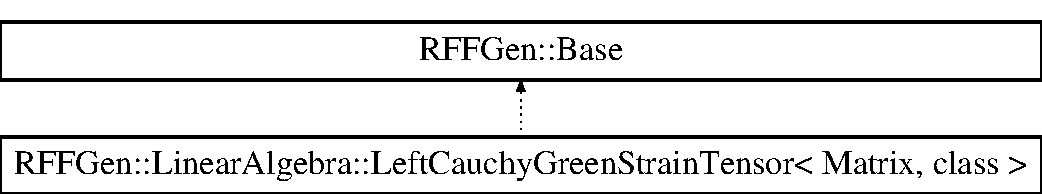
\includegraphics[height=0.898876cm]{classRFFGen_1_1LinearAlgebra_1_1LeftCauchyGreenStrainTensor}
\end{center}
\end{figure}
\subsection*{Public Member Functions}
\begin{DoxyCompactItemize}
\item 
\hyperlink{classRFFGen_1_1LinearAlgebra_1_1LeftCauchyGreenStrainTensor_a7cc082254e1cd5ef9bcd80e984adac9b}{Left\-Cauchy\-Green\-Strain\-Tensor} (Matrix const \&F)
\begin{DoxyCompactList}\small\item\em Constructor. \end{DoxyCompactList}\item 
\hypertarget{classRFFGen_1_1LinearAlgebra_1_1LeftCauchyGreenStrainTensor_a73dbd1543b5f4bf0c13b23b9962fc222}{void \hyperlink{classRFFGen_1_1LinearAlgebra_1_1LeftCauchyGreenStrainTensor_a73dbd1543b5f4bf0c13b23b9962fc222}{update} (Matrix const \&F)}\label{classRFFGen_1_1LinearAlgebra_1_1LeftCauchyGreenStrainTensor_a73dbd1543b5f4bf0c13b23b9962fc222}

\begin{DoxyCompactList}\small\item\em Reset point of evaluation. \end{DoxyCompactList}\item 
\hypertarget{classRFFGen_1_1LinearAlgebra_1_1LeftCauchyGreenStrainTensor_a5306342041dd2fc8a24863b6a0cc7368}{Matrix const \& \hyperlink{classRFFGen_1_1LinearAlgebra_1_1LeftCauchyGreenStrainTensor_a5306342041dd2fc8a24863b6a0cc7368}{d0} () const noexcept}\label{classRFFGen_1_1LinearAlgebra_1_1LeftCauchyGreenStrainTensor_a5306342041dd2fc8a24863b6a0cc7368}

\begin{DoxyCompactList}\small\item\em Function value $ F^T * F $. \end{DoxyCompactList}\item 
\hypertarget{classRFFGen_1_1LinearAlgebra_1_1LeftCauchyGreenStrainTensor_a3a49e4c9105a4a466c43d5cd262fe725}{{\footnotesize template$<$int $>$ }\\Matrix \hyperlink{classRFFGen_1_1LinearAlgebra_1_1LeftCauchyGreenStrainTensor_a3a49e4c9105a4a466c43d5cd262fe725}{d1} (Matrix const \&d\-F1) const }\label{classRFFGen_1_1LinearAlgebra_1_1LeftCauchyGreenStrainTensor_a3a49e4c9105a4a466c43d5cd262fe725}

\begin{DoxyCompactList}\small\item\em First directional derivative $ F^T dF_1 + dF_1^T F $. \end{DoxyCompactList}\item 
\hypertarget{classRFFGen_1_1LinearAlgebra_1_1LeftCauchyGreenStrainTensor_ad15848883104beb2265dfb459d96dff2}{{\footnotesize template$<$int , int $>$ }\\Matrix \hyperlink{classRFFGen_1_1LinearAlgebra_1_1LeftCauchyGreenStrainTensor_ad15848883104beb2265dfb459d96dff2}{d2} (Matrix const \&d\-F1, Matrix const \&d\-F2) const }\label{classRFFGen_1_1LinearAlgebra_1_1LeftCauchyGreenStrainTensor_ad15848883104beb2265dfb459d96dff2}

\begin{DoxyCompactList}\small\item\em Second directional derivative $ dF_2^T dF_1 + dF_1^T dF_2 $. \end{DoxyCompactList}\end{DoxyCompactItemize}


\subsection{Detailed Description}
\subsubsection*{template$<$class Matrix, class = Concepts\-::\-Symmetric\-Matrix\-Concept\-Check$<$\-Matrix$>$$>$class R\-F\-F\-Gen\-::\-Linear\-Algebra\-::\-Left\-Cauchy\-Green\-Strain\-Tensor$<$ Matrix, class $>$}

Left Cauchy-\/\-Green strain tensor $ F^T F $ for a symmetric matrix $ F $. 

This class is used for nonlinear material models based on the deformation gradient $\nabla\varphi$, which takes the role of $F$. Caches both $ F^T $ and $ F^T F $. 

\subsection{Constructor \& Destructor Documentation}
\hypertarget{classRFFGen_1_1LinearAlgebra_1_1LeftCauchyGreenStrainTensor_a7cc082254e1cd5ef9bcd80e984adac9b}{\index{R\-F\-F\-Gen\-::\-Linear\-Algebra\-::\-Left\-Cauchy\-Green\-Strain\-Tensor@{R\-F\-F\-Gen\-::\-Linear\-Algebra\-::\-Left\-Cauchy\-Green\-Strain\-Tensor}!Left\-Cauchy\-Green\-Strain\-Tensor@{Left\-Cauchy\-Green\-Strain\-Tensor}}
\index{Left\-Cauchy\-Green\-Strain\-Tensor@{Left\-Cauchy\-Green\-Strain\-Tensor}!RFFGen::LinearAlgebra::LeftCauchyGreenStrainTensor@{R\-F\-F\-Gen\-::\-Linear\-Algebra\-::\-Left\-Cauchy\-Green\-Strain\-Tensor}}
\subsubsection[{Left\-Cauchy\-Green\-Strain\-Tensor}]{\setlength{\rightskip}{0pt plus 5cm}template$<$class Matrix , class  = Concepts\-::\-Symmetric\-Matrix\-Concept\-Check$<$\-Matrix$>$$>$ {\bf R\-F\-F\-Gen\-::\-Linear\-Algebra\-::\-Left\-Cauchy\-Green\-Strain\-Tensor}$<$ Matrix, class $>$\-::{\bf Left\-Cauchy\-Green\-Strain\-Tensor} (
\begin{DoxyParamCaption}
\item[{Matrix const \&}]{F}
\end{DoxyParamCaption}
)\hspace{0.3cm}{\ttfamily [inline]}, {\ttfamily [explicit]}}}\label{classRFFGen_1_1LinearAlgebra_1_1LeftCauchyGreenStrainTensor_a7cc082254e1cd5ef9bcd80e984adac9b}


Constructor. 


\begin{DoxyParams}{Parameters}
{\em F} & point of evaluation. \\
\hline
\end{DoxyParams}


The documentation for this class was generated from the following file\-:\begin{DoxyCompactItemize}
\item 
R\-F\-F\-Gen/\-Linear\-Algebra/strain\-Tensor.\-hh\end{DoxyCompactItemize}

\hypertarget{classRFFGen_1_1LinearAlgebra_1_1LinearizedStrainTensor}{\section{R\-F\-F\-Gen\-:\-:Linear\-Algebra\-:\-:Linearized\-Strain\-Tensor$<$ Matrix, class $>$ Class Template Reference}
\label{classRFFGen_1_1LinearAlgebra_1_1LinearizedStrainTensor}\index{R\-F\-F\-Gen\-::\-Linear\-Algebra\-::\-Linearized\-Strain\-Tensor$<$ Matrix, class $>$@{R\-F\-F\-Gen\-::\-Linear\-Algebra\-::\-Linearized\-Strain\-Tensor$<$ Matrix, class $>$}}
}


Linearized strain tensor $ \frac{1}{2}\left(F^T+F\right) $.  




{\ttfamily \#include $<$strain\-Tensor.\-hh$>$}

Inheritance diagram for R\-F\-F\-Gen\-:\-:Linear\-Algebra\-:\-:Linearized\-Strain\-Tensor$<$ Matrix, class $>$\-:\begin{figure}[H]
\begin{center}
\leavevmode
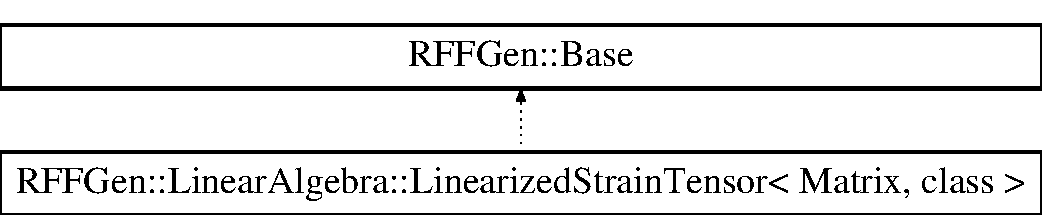
\includegraphics[height=2.000000cm]{classRFFGen_1_1LinearAlgebra_1_1LinearizedStrainTensor}
\end{center}
\end{figure}
\subsection*{Public Member Functions}
\begin{DoxyCompactItemize}
\item 
\hyperlink{classRFFGen_1_1LinearAlgebra_1_1LinearizedStrainTensor_a70feeb97bdd239df94760da3ee493a44}{Linearized\-Strain\-Tensor} (const Matrix \&F)
\begin{DoxyCompactList}\small\item\em Constructor. \end{DoxyCompactList}\item 
\hypertarget{classRFFGen_1_1LinearAlgebra_1_1LinearizedStrainTensor_a56675ad7e1c0cf4f4c92fb06b4b003b5}{void \hyperlink{classRFFGen_1_1LinearAlgebra_1_1LinearizedStrainTensor_a56675ad7e1c0cf4f4c92fb06b4b003b5}{update} (Matrix const \&F)}\label{classRFFGen_1_1LinearAlgebra_1_1LinearizedStrainTensor_a56675ad7e1c0cf4f4c92fb06b4b003b5}

\begin{DoxyCompactList}\small\item\em Reset point of evaluation. \end{DoxyCompactList}\item 
\hypertarget{classRFFGen_1_1LinearAlgebra_1_1LinearizedStrainTensor_a12078ba0d36e115a44b126b0c22b9773}{Matrix const \& \hyperlink{classRFFGen_1_1LinearAlgebra_1_1LinearizedStrainTensor_a12078ba0d36e115a44b126b0c22b9773}{d0} () const }\label{classRFFGen_1_1LinearAlgebra_1_1LinearizedStrainTensor_a12078ba0d36e115a44b126b0c22b9773}

\begin{DoxyCompactList}\small\item\em Function value $ \frac{1}{2}\left(F^T+F\right) $. \end{DoxyCompactList}\item 
\hypertarget{classRFFGen_1_1LinearAlgebra_1_1LinearizedStrainTensor_a62288bd627caf2cf7878d7eed0856d13}{{\footnotesize template$<$int $>$ }\\Matrix \hyperlink{classRFFGen_1_1LinearAlgebra_1_1LinearizedStrainTensor_a62288bd627caf2cf7878d7eed0856d13}{d1} (const Matrix \&d\-F) const }\label{classRFFGen_1_1LinearAlgebra_1_1LinearizedStrainTensor_a62288bd627caf2cf7878d7eed0856d13}

\begin{DoxyCompactList}\small\item\em First directional derivative $ \frac{1}{2}\left(dF^T+dF\right) $. \end{DoxyCompactList}\end{DoxyCompactItemize}


\subsection{Detailed Description}
\subsubsection*{template$<$class Matrix, class = Concepts\-::\-Symmetric\-Matrix\-Concept\-Check$<$\-Matrix$>$$>$class R\-F\-F\-Gen\-::\-Linear\-Algebra\-::\-Linearized\-Strain\-Tensor$<$ Matrix, class $>$}

Linearized strain tensor $ \frac{1}{2}\left(F^T+F\right) $. 

This class is used for linear material models based on the displacement gradient $\nabla u$, which takes the role of $F$. Caches the function value $ \frac{1}{2}\left(F^T+F\right) $. 

\subsection{Constructor \& Destructor Documentation}
\hypertarget{classRFFGen_1_1LinearAlgebra_1_1LinearizedStrainTensor_a70feeb97bdd239df94760da3ee493a44}{\index{R\-F\-F\-Gen\-::\-Linear\-Algebra\-::\-Linearized\-Strain\-Tensor@{R\-F\-F\-Gen\-::\-Linear\-Algebra\-::\-Linearized\-Strain\-Tensor}!Linearized\-Strain\-Tensor@{Linearized\-Strain\-Tensor}}
\index{Linearized\-Strain\-Tensor@{Linearized\-Strain\-Tensor}!RFFGen::LinearAlgebra::LinearizedStrainTensor@{R\-F\-F\-Gen\-::\-Linear\-Algebra\-::\-Linearized\-Strain\-Tensor}}
\subsubsection[{Linearized\-Strain\-Tensor}]{\setlength{\rightskip}{0pt plus 5cm}template$<$class Matrix, class  = Concepts\-::\-Symmetric\-Matrix\-Concept\-Check$<$\-Matrix$>$$>$ {\bf R\-F\-F\-Gen\-::\-Linear\-Algebra\-::\-Linearized\-Strain\-Tensor}$<$ Matrix, class $>$\-::{\bf Linearized\-Strain\-Tensor} (
\begin{DoxyParamCaption}
\item[{const Matrix \&}]{F}
\end{DoxyParamCaption}
)\hspace{0.3cm}{\ttfamily [inline]}, {\ttfamily [explicit]}}}\label{classRFFGen_1_1LinearAlgebra_1_1LinearizedStrainTensor_a70feeb97bdd239df94760da3ee493a44}


Constructor. 


\begin{DoxyParams}{Parameters}
{\em F} & point of evaluation \\
\hline
\end{DoxyParams}


The documentation for this class was generated from the following file\-:\begin{DoxyCompactItemize}
\item 
R\-F\-F\-Gen/\-Linear\-Algebra/strain\-Tensor.\-hh\end{DoxyCompactItemize}

\hypertarget{structRFFGen_1_1CMath_1_1LN}{\section{R\-F\-F\-Gen\-:\-:C\-Math\-:\-:L\-N Struct Reference}
\label{structRFFGen_1_1CMath_1_1LN}\index{R\-F\-F\-Gen\-::\-C\-Math\-::\-L\-N@{R\-F\-F\-Gen\-::\-C\-Math\-::\-L\-N}}
}


Natural logarithm including first three derivatives.  




{\ttfamily \#include $<$log.\-hh$>$}

Inheritance diagram for R\-F\-F\-Gen\-:\-:C\-Math\-:\-:L\-N\-:\begin{figure}[H]
\begin{center}
\leavevmode
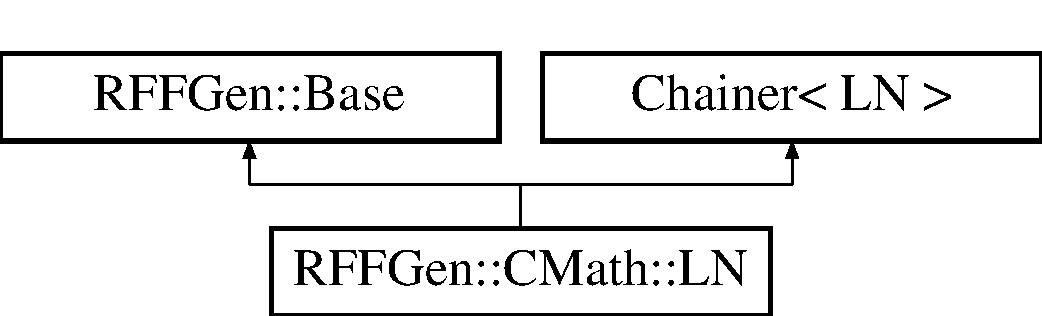
\includegraphics[height=2.000000cm]{structRFFGen_1_1CMath_1_1LN}
\end{center}
\end{figure}
\subsection*{Public Member Functions}
\begin{DoxyCompactItemize}
\item 
\hyperlink{structRFFGen_1_1CMath_1_1LN_a9075257a79e80959bc6a5f4554e7eb3c}{L\-N} (double x=1.)
\begin{DoxyCompactList}\small\item\em Constructor. \end{DoxyCompactList}\item 
\hypertarget{structRFFGen_1_1CMath_1_1LN_a7beffe12125854592fff89a0d5ba3cc1}{void \hyperlink{structRFFGen_1_1CMath_1_1LN_a7beffe12125854592fff89a0d5ba3cc1}{update} (double x)}\label{structRFFGen_1_1CMath_1_1LN_a7beffe12125854592fff89a0d5ba3cc1}

\begin{DoxyCompactList}\small\item\em Reset point of evaluation. \end{DoxyCompactList}\item 
\hypertarget{structRFFGen_1_1CMath_1_1LN_a22ec7b2086752cba9582c91c99f5d19a}{double \hyperlink{structRFFGen_1_1CMath_1_1LN_a22ec7b2086752cba9582c91c99f5d19a}{d0} () const noexcept}\label{structRFFGen_1_1CMath_1_1LN_a22ec7b2086752cba9582c91c99f5d19a}

\begin{DoxyCompactList}\small\item\em Function value. \end{DoxyCompactList}\item 
\hypertarget{structRFFGen_1_1CMath_1_1LN_a7c178c972e191e40f75f0387d275c518}{{\footnotesize template$<$int  = -\/1$>$ }\\double \hyperlink{structRFFGen_1_1CMath_1_1LN_a7c178c972e191e40f75f0387d275c518}{d1} (double dx=1.) const }\label{structRFFGen_1_1CMath_1_1LN_a7c178c972e191e40f75f0387d275c518}

\begin{DoxyCompactList}\small\item\em First (directional) derivative. \end{DoxyCompactList}\item 
\hypertarget{structRFFGen_1_1CMath_1_1LN_abf73d04c03868d0cb07a1bb764a90456}{{\footnotesize template$<$int  = -\/1, int  = -\/1$>$ }\\double \hyperlink{structRFFGen_1_1CMath_1_1LN_abf73d04c03868d0cb07a1bb764a90456}{d2} (double dx=1., double dy=1.) const }\label{structRFFGen_1_1CMath_1_1LN_abf73d04c03868d0cb07a1bb764a90456}

\begin{DoxyCompactList}\small\item\em Second (directional) derivative. \end{DoxyCompactList}\item 
\hypertarget{structRFFGen_1_1CMath_1_1LN_ae0afaeb6f05e8176b28b14ca088728f1}{{\footnotesize template$<$int  = -\/1, int  = -\/1, int  = -\/1$>$ }\\double \hyperlink{structRFFGen_1_1CMath_1_1LN_ae0afaeb6f05e8176b28b14ca088728f1}{d3} (double dx=1., double dy=1., double dz=1.) const }\label{structRFFGen_1_1CMath_1_1LN_ae0afaeb6f05e8176b28b14ca088728f1}

\begin{DoxyCompactList}\small\item\em Third (directional) derivative. \end{DoxyCompactList}\end{DoxyCompactItemize}


\subsection{Detailed Description}
Natural logarithm including first three derivatives. 

For scalar functions directional derivatives are less interesting. Incorporating this function as building block for more complex functions requires directional derivatives. These occur during applications of the chain rule. 

\subsection{Constructor \& Destructor Documentation}
\hypertarget{structRFFGen_1_1CMath_1_1LN_a9075257a79e80959bc6a5f4554e7eb3c}{\index{R\-F\-F\-Gen\-::\-C\-Math\-::\-L\-N@{R\-F\-F\-Gen\-::\-C\-Math\-::\-L\-N}!L\-N@{L\-N}}
\index{L\-N@{L\-N}!RFFGen::CMath::LN@{R\-F\-F\-Gen\-::\-C\-Math\-::\-L\-N}}
\subsubsection[{L\-N}]{\setlength{\rightskip}{0pt plus 5cm}R\-F\-F\-Gen\-::\-C\-Math\-::\-L\-N\-::\-L\-N (
\begin{DoxyParamCaption}
\item[{double}]{x = {\ttfamily 1.}}
\end{DoxyParamCaption}
)\hspace{0.3cm}{\ttfamily [inline]}, {\ttfamily [explicit]}}}\label{structRFFGen_1_1CMath_1_1LN_a9075257a79e80959bc6a5f4554e7eb3c}


Constructor. 


\begin{DoxyParams}{Parameters}
{\em x} & point of evaluation. \\
\hline
\end{DoxyParams}


The documentation for this struct was generated from the following file\-:\begin{DoxyCompactItemize}
\item 
R\-F\-F\-Gen/\-C\-Math/log.\-hh\end{DoxyCompactItemize}

\hypertarget{structRFFGen_1_1CMath_1_1Log10}{\section{R\-F\-F\-Gen\-:\-:C\-Math\-:\-:Log10 Struct Reference}
\label{structRFFGen_1_1CMath_1_1Log10}\index{R\-F\-F\-Gen\-::\-C\-Math\-::\-Log10@{R\-F\-F\-Gen\-::\-C\-Math\-::\-Log10}}
}


Common (base 10) logarithm including first three derivatives.  




{\ttfamily \#include $<$log.\-hh$>$}

Inheritance diagram for R\-F\-F\-Gen\-:\-:C\-Math\-:\-:Log10\-:\begin{figure}[H]
\begin{center}
\leavevmode
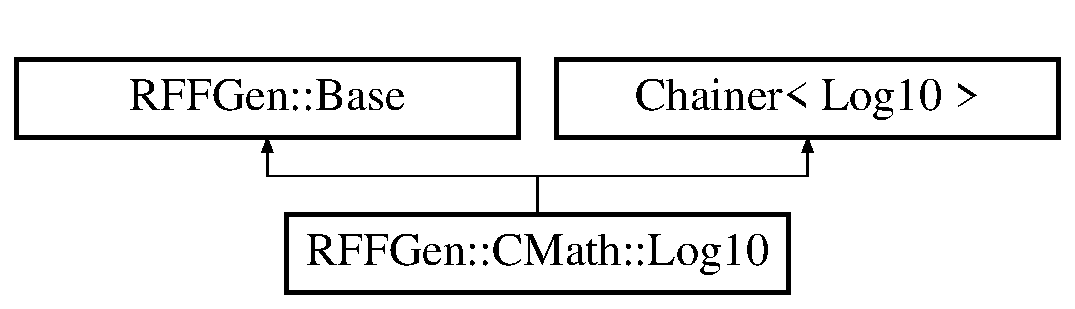
\includegraphics[height=2.000000cm]{structRFFGen_1_1CMath_1_1Log10}
\end{center}
\end{figure}
\subsection*{Public Member Functions}
\begin{DoxyCompactItemize}
\item 
\hyperlink{structRFFGen_1_1CMath_1_1Log10_a34ec695de7574539a7ab0c9f82773aee}{Log10} (double x=1.)
\begin{DoxyCompactList}\small\item\em Constructor. \end{DoxyCompactList}\item 
\hypertarget{structRFFGen_1_1CMath_1_1Log10_a30722b597e5b2cc7a38518fff7abb87a}{void \hyperlink{structRFFGen_1_1CMath_1_1Log10_a30722b597e5b2cc7a38518fff7abb87a}{update} (double x)}\label{structRFFGen_1_1CMath_1_1Log10_a30722b597e5b2cc7a38518fff7abb87a}

\begin{DoxyCompactList}\small\item\em Reset point of evaluation. \end{DoxyCompactList}\item 
\hypertarget{structRFFGen_1_1CMath_1_1Log10_a7f8d8fe13e5f3287a8b4baef1b29b600}{double \hyperlink{structRFFGen_1_1CMath_1_1Log10_a7f8d8fe13e5f3287a8b4baef1b29b600}{d0} () const noexcept}\label{structRFFGen_1_1CMath_1_1Log10_a7f8d8fe13e5f3287a8b4baef1b29b600}

\begin{DoxyCompactList}\small\item\em Function value. \end{DoxyCompactList}\item 
\hypertarget{structRFFGen_1_1CMath_1_1Log10_a80064263bb47d44403dd4725279ff5e8}{{\footnotesize template$<$int  = -\/1$>$ }\\double \hyperlink{structRFFGen_1_1CMath_1_1Log10_a80064263bb47d44403dd4725279ff5e8}{d1} (double dx=1.) const }\label{structRFFGen_1_1CMath_1_1Log10_a80064263bb47d44403dd4725279ff5e8}

\begin{DoxyCompactList}\small\item\em First (directional) derivative. \end{DoxyCompactList}\item 
\hypertarget{structRFFGen_1_1CMath_1_1Log10_aa53762004f57b286a20fd3b91d1ecb3d}{{\footnotesize template$<$int  = -\/1, int  = -\/1$>$ }\\double \hyperlink{structRFFGen_1_1CMath_1_1Log10_aa53762004f57b286a20fd3b91d1ecb3d}{d2} (double dx=1., double dy=1.) const }\label{structRFFGen_1_1CMath_1_1Log10_aa53762004f57b286a20fd3b91d1ecb3d}

\begin{DoxyCompactList}\small\item\em Second (directional) derivative. \end{DoxyCompactList}\item 
\hypertarget{structRFFGen_1_1CMath_1_1Log10_a2e17aff475d70c644428cc8303eab24f}{{\footnotesize template$<$int  = -\/1, int  = -\/1, int  = -\/1$>$ }\\double \hyperlink{structRFFGen_1_1CMath_1_1Log10_a2e17aff475d70c644428cc8303eab24f}{d3} (double dx=1., double dy=1., double dz=1.) const }\label{structRFFGen_1_1CMath_1_1Log10_a2e17aff475d70c644428cc8303eab24f}

\begin{DoxyCompactList}\small\item\em Third (directional) derivative. \end{DoxyCompactList}\end{DoxyCompactItemize}


\subsection{Detailed Description}
Common (base 10) logarithm including first three derivatives. 

For scalar functions directional derivatives are less interesting. Incorporating this function as building block for more complex functions requires directional derivatives. These occur during applications of the chain rule. 

\subsection{Constructor \& Destructor Documentation}
\hypertarget{structRFFGen_1_1CMath_1_1Log10_a34ec695de7574539a7ab0c9f82773aee}{\index{R\-F\-F\-Gen\-::\-C\-Math\-::\-Log10@{R\-F\-F\-Gen\-::\-C\-Math\-::\-Log10}!Log10@{Log10}}
\index{Log10@{Log10}!RFFGen::CMath::Log10@{R\-F\-F\-Gen\-::\-C\-Math\-::\-Log10}}
\subsubsection[{Log10}]{\setlength{\rightskip}{0pt plus 5cm}R\-F\-F\-Gen\-::\-C\-Math\-::\-Log10\-::\-Log10 (
\begin{DoxyParamCaption}
\item[{double}]{x = {\ttfamily 1.}}
\end{DoxyParamCaption}
)\hspace{0.3cm}{\ttfamily [inline]}, {\ttfamily [explicit]}}}\label{structRFFGen_1_1CMath_1_1Log10_a34ec695de7574539a7ab0c9f82773aee}


Constructor. 


\begin{DoxyParams}{Parameters}
{\em x} & point of evaluation. \\
\hline
\end{DoxyParams}


The documentation for this struct was generated from the following file\-:\begin{DoxyCompactItemize}
\item 
R\-F\-F\-Gen/\-C\-Math/log.\-hh\end{DoxyCompactItemize}

\hypertarget{structRFFGen_1_1CMath_1_1Log2}{\section{R\-F\-F\-Gen\-:\-:C\-Math\-:\-:Log2 Struct Reference}
\label{structRFFGen_1_1CMath_1_1Log2}\index{R\-F\-F\-Gen\-::\-C\-Math\-::\-Log2@{R\-F\-F\-Gen\-::\-C\-Math\-::\-Log2}}
}


Base 2 logarithm including first three derivatives.  




{\ttfamily \#include $<$log.\-hh$>$}

Inheritance diagram for R\-F\-F\-Gen\-:\-:C\-Math\-:\-:Log2\-:\begin{figure}[H]
\begin{center}
\leavevmode
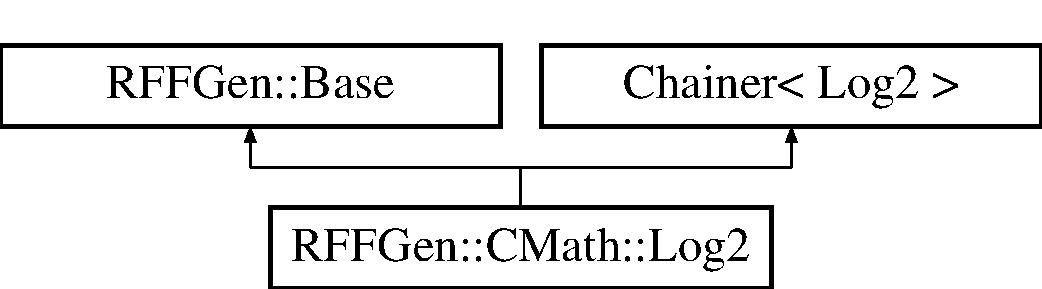
\includegraphics[height=2.000000cm]{structRFFGen_1_1CMath_1_1Log2}
\end{center}
\end{figure}
\subsection*{Public Member Functions}
\begin{DoxyCompactItemize}
\item 
\hyperlink{structRFFGen_1_1CMath_1_1Log2_a06c05ea7727a6f2671ca4c044589c155}{Log2} (double x=1.)
\begin{DoxyCompactList}\small\item\em Constructor. \end{DoxyCompactList}\item 
\hypertarget{structRFFGen_1_1CMath_1_1Log2_af7d232fd86acfcfce9cb26373051a7b7}{void \hyperlink{structRFFGen_1_1CMath_1_1Log2_af7d232fd86acfcfce9cb26373051a7b7}{update} (double x)}\label{structRFFGen_1_1CMath_1_1Log2_af7d232fd86acfcfce9cb26373051a7b7}

\begin{DoxyCompactList}\small\item\em Reset point of evaluation. \end{DoxyCompactList}\item 
\hypertarget{structRFFGen_1_1CMath_1_1Log2_abbfa6f5dca5bfc1293469c2909561196}{double \hyperlink{structRFFGen_1_1CMath_1_1Log2_abbfa6f5dca5bfc1293469c2909561196}{d0} () const noexcept}\label{structRFFGen_1_1CMath_1_1Log2_abbfa6f5dca5bfc1293469c2909561196}

\begin{DoxyCompactList}\small\item\em Function value. \end{DoxyCompactList}\item 
\hypertarget{structRFFGen_1_1CMath_1_1Log2_ab496ec15aa694d16e76aa91aacfeba87}{{\footnotesize template$<$int  = -\/1$>$ }\\double \hyperlink{structRFFGen_1_1CMath_1_1Log2_ab496ec15aa694d16e76aa91aacfeba87}{d1} (double dx=1.) const }\label{structRFFGen_1_1CMath_1_1Log2_ab496ec15aa694d16e76aa91aacfeba87}

\begin{DoxyCompactList}\small\item\em First (directional) derivative. \end{DoxyCompactList}\item 
\hypertarget{structRFFGen_1_1CMath_1_1Log2_a286d4b77ec5f7012f6391dfd8975b198}{{\footnotesize template$<$int  = -\/1, int  = -\/1$>$ }\\double \hyperlink{structRFFGen_1_1CMath_1_1Log2_a286d4b77ec5f7012f6391dfd8975b198}{d2} (double dx=1., double dy=1.) const }\label{structRFFGen_1_1CMath_1_1Log2_a286d4b77ec5f7012f6391dfd8975b198}

\begin{DoxyCompactList}\small\item\em Second (directional) derivative. \end{DoxyCompactList}\item 
\hypertarget{structRFFGen_1_1CMath_1_1Log2_a6c04e67e1b9dd2e590f9e60936093019}{{\footnotesize template$<$int  = -\/1, int  = -\/1, int  = -\/1$>$ }\\double \hyperlink{structRFFGen_1_1CMath_1_1Log2_a6c04e67e1b9dd2e590f9e60936093019}{d3} (double dx=1., double dy=1., double dz=1.) const }\label{structRFFGen_1_1CMath_1_1Log2_a6c04e67e1b9dd2e590f9e60936093019}

\begin{DoxyCompactList}\small\item\em Third (directional) derivative. \end{DoxyCompactList}\end{DoxyCompactItemize}


\subsection{Detailed Description}
Base 2 logarithm including first three derivatives. 

For scalar functions directional derivatives are less interesting. Incorporating this function as building block for more complex functions requires directional derivatives. These occur during applications of the chain rule. 

\subsection{Constructor \& Destructor Documentation}
\hypertarget{structRFFGen_1_1CMath_1_1Log2_a06c05ea7727a6f2671ca4c044589c155}{\index{R\-F\-F\-Gen\-::\-C\-Math\-::\-Log2@{R\-F\-F\-Gen\-::\-C\-Math\-::\-Log2}!Log2@{Log2}}
\index{Log2@{Log2}!RFFGen::CMath::Log2@{R\-F\-F\-Gen\-::\-C\-Math\-::\-Log2}}
\subsubsection[{Log2}]{\setlength{\rightskip}{0pt plus 5cm}R\-F\-F\-Gen\-::\-C\-Math\-::\-Log2\-::\-Log2 (
\begin{DoxyParamCaption}
\item[{double}]{x = {\ttfamily 1.}}
\end{DoxyParamCaption}
)\hspace{0.3cm}{\ttfamily [inline]}, {\ttfamily [explicit]}}}\label{structRFFGen_1_1CMath_1_1Log2_a06c05ea7727a6f2671ca4c044589c155}


Constructor. 


\begin{DoxyParams}{Parameters}
{\em x} & point of evaluation. \\
\hline
\end{DoxyParams}


The documentation for this struct was generated from the following file\-:\begin{DoxyCompactItemize}
\item 
R\-F\-F\-Gen/\-C\-Math/log.\-hh\end{DoxyCompactItemize}

\hypertarget{structRFFGen_1_1Concepts_1_1MatrixConcept}{\section{R\-F\-F\-Gen\-:\-:Concepts\-:\-:Matrix\-Concept Struct Reference}
\label{structRFFGen_1_1Concepts_1_1MatrixConcept}\index{R\-F\-F\-Gen\-::\-Concepts\-::\-Matrix\-Concept@{R\-F\-F\-Gen\-::\-Concepts\-::\-Matrix\-Concept}}
}


Requirements for matrices.  




{\ttfamily \#include $<$concepts.\-hh$>$}

Inheritance diagram for R\-F\-F\-Gen\-:\-:Concepts\-:\-:Matrix\-Concept\-:\begin{figure}[H]
\begin{center}
\leavevmode
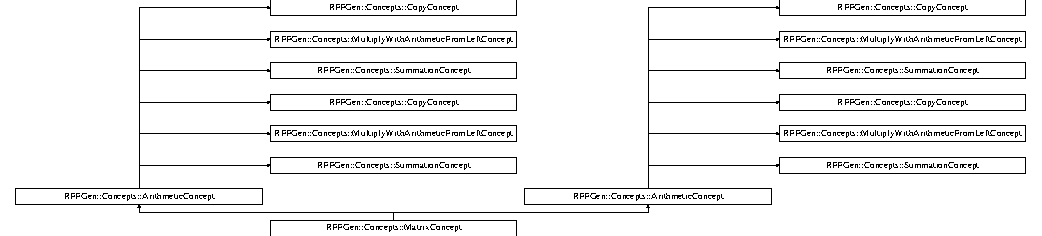
\includegraphics[height=1.586402cm]{structRFFGen_1_1Concepts_1_1MatrixConcept}
\end{center}
\end{figure}
\subsection*{Public Member Functions}
\begin{DoxyCompactItemize}
\item 
\hypertarget{structRFFGen_1_1Concepts_1_1MatrixConcept_a9edaafd682629e350028a6d943f98a2d}{unspecified \hyperlink{structRFFGen_1_1Concepts_1_1MatrixConcept_a9edaafd682629e350028a6d943f98a2d}{operator\mbox{[}$\,$\mbox{]}} (int)}\label{structRFFGen_1_1Concepts_1_1MatrixConcept_a9edaafd682629e350028a6d943f98a2d}

\begin{DoxyCompactList}\small\item\em Access to row, providing itself the same \hyperlink{structRFFGen_1_1Concepts_1_1MatrixConcept_a9edaafd682629e350028a6d943f98a2d}{operator\mbox{[}$\,$\mbox{]}(int)}. \end{DoxyCompactList}\item 
\hypertarget{structRFFGen_1_1Concepts_1_1MatrixConcept_a2f067ad171c8a9678b77fea11b6e7ec4}{unspecified \hyperlink{structRFFGen_1_1Concepts_1_1MatrixConcept_a2f067ad171c8a9678b77fea11b6e7ec4}{operator()} (int, int)}\label{structRFFGen_1_1Concepts_1_1MatrixConcept_a2f067ad171c8a9678b77fea11b6e7ec4}

\begin{DoxyCompactList}\small\item\em Access to entry. \end{DoxyCompactList}\end{DoxyCompactItemize}


\subsection{Detailed Description}
Requirements for matrices. 

Access to matrix elements must be possible either via A\mbox{[}i\mbox{]}\mbox{[}j\mbox{]} or A(i,j). Moreover the requirements of \hyperlink{structRFFGen_1_1Concepts_1_1ArithmeticConcept}{Arithmetic\-Concept} must be satisfied. 

The documentation for this struct was generated from the following file\-:\begin{DoxyCompactItemize}
\item 
R\-F\-F\-Gen/\hyperlink{concepts_8hh}{concepts.\-hh}\end{DoxyCompactItemize}

\hypertarget{structRFFGen_1_1Concepts_1_1MatrixConceptCheck}{\section{R\-F\-F\-Gen\-:\-:Concepts\-:\-:Matrix\-Concept\-Check$<$ Matrix $>$ Struct Template Reference}
\label{structRFFGen_1_1Concepts_1_1MatrixConceptCheck}\index{R\-F\-F\-Gen\-::\-Concepts\-::\-Matrix\-Concept\-Check$<$ Matrix $>$@{R\-F\-F\-Gen\-::\-Concepts\-::\-Matrix\-Concept\-Check$<$ Matrix $>$}}
}


Static check if the requirements of \hyperlink{structRFFGen_1_1Concepts_1_1MatrixConcept}{Matrix\-Concept} are satisfied.  




{\ttfamily \#include $<$concept\-Check.\-hh$>$}

Inheritance diagram for R\-F\-F\-Gen\-:\-:Concepts\-:\-:Matrix\-Concept\-Check$<$ Matrix $>$\-:\begin{figure}[H]
\begin{center}
\leavevmode
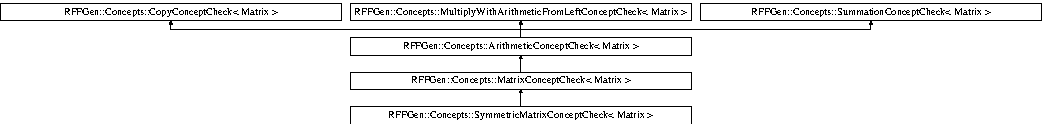
\includegraphics[height=1.666667cm]{structRFFGen_1_1Concepts_1_1MatrixConceptCheck}
\end{center}
\end{figure}


\subsection{Detailed Description}
\subsubsection*{template$<$class Matrix$>$struct R\-F\-F\-Gen\-::\-Concepts\-::\-Matrix\-Concept\-Check$<$ Matrix $>$}

Static check if the requirements of \hyperlink{structRFFGen_1_1Concepts_1_1MatrixConcept}{Matrix\-Concept} are satisfied. 

The documentation for this struct was generated from the following file\-:\begin{DoxyCompactItemize}
\item 
R\-F\-F\-Gen/concept\-Check.\-hh\end{DoxyCompactItemize}

\hypertarget{structRFFGen_1_1Concepts_1_1MultiplicationConcept}{\section{R\-F\-F\-Gen\-:\-:Concepts\-:\-:Multiplication\-Concept Struct Reference}
\label{structRFFGen_1_1Concepts_1_1MultiplicationConcept}\index{R\-F\-F\-Gen\-::\-Concepts\-::\-Multiplication\-Concept@{R\-F\-F\-Gen\-::\-Concepts\-::\-Multiplication\-Concept}}
}


Requires that multiplication can be performed.  




{\ttfamily \#include $<$concepts.\-hh$>$}

\subsection*{Public Member Functions}
\begin{DoxyCompactItemize}
\item 
\hypertarget{structRFFGen_1_1Concepts_1_1MultiplicationConcept_a65cf060bcfd7bd39b527de6c87056539}{unspecified \hyperlink{structRFFGen_1_1Concepts_1_1MultiplicationConcept_a65cf060bcfd7bd39b527de6c87056539}{operator$\ast$=} (Arg2)}\label{structRFFGen_1_1Concepts_1_1MultiplicationConcept_a65cf060bcfd7bd39b527de6c87056539}

\begin{DoxyCompactList}\small\item\em In-\/place multiplication. Return type is not checked to support lazy evaluation. \end{DoxyCompactList}\item 
\hypertarget{structRFFGen_1_1Concepts_1_1MultiplicationConcept_ae876451286ab0e902a5cec841ad01f2e}{unspecified \hyperlink{structRFFGen_1_1Concepts_1_1MultiplicationConcept_ae876451286ab0e902a5cec841ad01f2e}{rightmultiplyany} (Arg2)}\label{structRFFGen_1_1Concepts_1_1MultiplicationConcept_ae876451286ab0e902a5cec841ad01f2e}

\begin{DoxyCompactList}\small\item\em Multiplication via \hyperlink{structRFFGen_1_1Concepts_1_1MultiplicationConcept_ae876451286ab0e902a5cec841ad01f2e}{rightmultiplyany(\-Arg2)}. Return type is not checked to support lazy evaluation. \end{DoxyCompactList}\item 
\hypertarget{structRFFGen_1_1Concepts_1_1MultiplicationConcept_a65cf060bcfd7bd39b527de6c87056539}{unspecified \hyperlink{structRFFGen_1_1Concepts_1_1MultiplicationConcept_a65cf060bcfd7bd39b527de6c87056539}{operator$\ast$=} (Arg2)}\label{structRFFGen_1_1Concepts_1_1MultiplicationConcept_a65cf060bcfd7bd39b527de6c87056539}

\begin{DoxyCompactList}\small\item\em In-\/place multiplication. Return type is not checked to support lazy evaluation. \end{DoxyCompactList}\item 
\hypertarget{structRFFGen_1_1Concepts_1_1MultiplicationConcept_ae876451286ab0e902a5cec841ad01f2e}{unspecified \hyperlink{structRFFGen_1_1Concepts_1_1MultiplicationConcept_ae876451286ab0e902a5cec841ad01f2e}{rightmultiplyany} (Arg2)}\label{structRFFGen_1_1Concepts_1_1MultiplicationConcept_ae876451286ab0e902a5cec841ad01f2e}

\begin{DoxyCompactList}\small\item\em Multiplication via \hyperlink{structRFFGen_1_1Concepts_1_1MultiplicationConcept_ae876451286ab0e902a5cec841ad01f2e}{rightmultiplyany(\-Arg2)}. Return type is not checked to support lazy evaluation. \end{DoxyCompactList}\end{DoxyCompactItemize}


\subsection{Detailed Description}
Requires that multiplication can be performed. 

Requires that either a free operator$\ast$(\-Arg1,\-Arg2) exists for multiplication or Arg1 provides either the in-\/place multiplication \hyperlink{structRFFGen_1_1Concepts_1_1MultiplicationConcept_a65cf060bcfd7bd39b527de6c87056539}{operator$\ast$=(\-Arg2)} or the member function \hyperlink{structRFFGen_1_1Concepts_1_1MultiplicationConcept_ae876451286ab0e902a5cec841ad01f2e}{rightmultiplyany(\-Arg2)}. 

The documentation for this struct was generated from the following file\-:\begin{DoxyCompactItemize}
\item 
concepts.\-hh\end{DoxyCompactItemize}

\hypertarget{structRFFGen_1_1Concepts_1_1MultiplicationConceptCheck}{\section{R\-F\-F\-Gen\-:\-:Concepts\-:\-:Multiplication\-Concept\-Check$<$ Arg1, Arg2 $>$ Struct Template Reference}
\label{structRFFGen_1_1Concepts_1_1MultiplicationConceptCheck}\index{R\-F\-F\-Gen\-::\-Concepts\-::\-Multiplication\-Concept\-Check$<$ Arg1, Arg2 $>$@{R\-F\-F\-Gen\-::\-Concepts\-::\-Multiplication\-Concept\-Check$<$ Arg1, Arg2 $>$}}
}


Static check if the requirements of \hyperlink{structRFFGen_1_1Concepts_1_1MultiplicationConcept}{Multiplication\-Concept} are satisfied.  




{\ttfamily \#include $<$concept\-Check.\-hh$>$}



\subsection{Detailed Description}
\subsubsection*{template$<$class Arg1, class Arg2$>$struct R\-F\-F\-Gen\-::\-Concepts\-::\-Multiplication\-Concept\-Check$<$ Arg1, Arg2 $>$}

Static check if the requirements of \hyperlink{structRFFGen_1_1Concepts_1_1MultiplicationConcept}{Multiplication\-Concept} are satisfied. 

The documentation for this struct was generated from the following file\-:\begin{DoxyCompactItemize}
\item 
R\-F\-F\-Gen/concept\-Check.\-hh\end{DoxyCompactItemize}

\hypertarget{structRFFGen_1_1Concepts_1_1MultiplyWithArithmeticFromLeftConcept}{\section{R\-F\-F\-Gen\-:\-:Concepts\-:\-:Multiply\-With\-Arithmetic\-From\-Left\-Concept Struct Reference}
\label{structRFFGen_1_1Concepts_1_1MultiplyWithArithmeticFromLeftConcept}\index{R\-F\-F\-Gen\-::\-Concepts\-::\-Multiply\-With\-Arithmetic\-From\-Left\-Concept@{R\-F\-F\-Gen\-::\-Concepts\-::\-Multiply\-With\-Arithmetic\-From\-Left\-Concept}}
}


Requires that multiplication with double and int can be performed either by in-\/place multiplication or by multiplication from the left.  




{\ttfamily \#include $<$concepts.\-hh$>$}

Inheritance diagram for R\-F\-F\-Gen\-:\-:Concepts\-:\-:Multiply\-With\-Arithmetic\-From\-Left\-Concept\-:\begin{figure}[H]
\begin{center}
\leavevmode
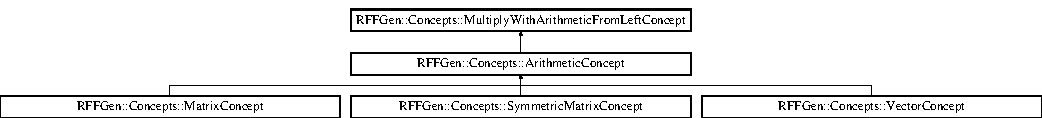
\includegraphics[height=3.172805cm]{structRFFGen_1_1Concepts_1_1MultiplyWithArithmeticFromLeftConcept}
\end{center}
\end{figure}
\subsection*{Public Member Functions}
\begin{DoxyCompactItemize}
\item 
\hypertarget{structRFFGen_1_1Concepts_1_1MultiplyWithArithmeticFromLeftConcept_ac7becd3ba4b0a7f81c2f83bfef9bad8c}{unspecified \hyperlink{structRFFGen_1_1Concepts_1_1MultiplyWithArithmeticFromLeftConcept_ac7becd3ba4b0a7f81c2f83bfef9bad8c}{operator$\ast$=} (double)}\label{structRFFGen_1_1Concepts_1_1MultiplyWithArithmeticFromLeftConcept_ac7becd3ba4b0a7f81c2f83bfef9bad8c}

\begin{DoxyCompactList}\small\item\em In-\/place multiplication. Return type is not checked to support lazy evaluation. \end{DoxyCompactList}\item 
\hypertarget{structRFFGen_1_1Concepts_1_1MultiplyWithArithmeticFromLeftConcept_af46b7b8e72ef559e6667e104ec745359}{unspecified \hyperlink{structRFFGen_1_1Concepts_1_1MultiplyWithArithmeticFromLeftConcept_af46b7b8e72ef559e6667e104ec745359}{operator$\ast$=} (int)}\label{structRFFGen_1_1Concepts_1_1MultiplyWithArithmeticFromLeftConcept_af46b7b8e72ef559e6667e104ec745359}

\begin{DoxyCompactList}\small\item\em In-\/place multiplication. Return type is not checked to support lazy evaluation. \end{DoxyCompactList}\item 
\hypertarget{structRFFGen_1_1Concepts_1_1MultiplyWithArithmeticFromLeftConcept_ac7becd3ba4b0a7f81c2f83bfef9bad8c}{unspecified \hyperlink{structRFFGen_1_1Concepts_1_1MultiplyWithArithmeticFromLeftConcept_ac7becd3ba4b0a7f81c2f83bfef9bad8c}{operator$\ast$=} (double)}\label{structRFFGen_1_1Concepts_1_1MultiplyWithArithmeticFromLeftConcept_ac7becd3ba4b0a7f81c2f83bfef9bad8c}

\begin{DoxyCompactList}\small\item\em In-\/place multiplication. Return type is not checked to support lazy evaluation. \end{DoxyCompactList}\item 
\hypertarget{structRFFGen_1_1Concepts_1_1MultiplyWithArithmeticFromLeftConcept_af46b7b8e72ef559e6667e104ec745359}{unspecified \hyperlink{structRFFGen_1_1Concepts_1_1MultiplyWithArithmeticFromLeftConcept_af46b7b8e72ef559e6667e104ec745359}{operator$\ast$=} (int)}\label{structRFFGen_1_1Concepts_1_1MultiplyWithArithmeticFromLeftConcept_af46b7b8e72ef559e6667e104ec745359}

\begin{DoxyCompactList}\small\item\em In-\/place multiplication. Return type is not checked to support lazy evaluation. \end{DoxyCompactList}\end{DoxyCompactItemize}


\subsection{Detailed Description}
Requires that multiplication with double and int can be performed either by in-\/place multiplication or by multiplication from the left. 


\begin{DoxyTemplParams}{Template Parameters}
{\em Arg} & type to check \\
\hline
\end{DoxyTemplParams}


The documentation for this struct was generated from the following file\-:\begin{DoxyCompactItemize}
\item 
concepts.\-hh\end{DoxyCompactItemize}

\hypertarget{structRFFGen_1_1Concepts_1_1MultiplyWithArithmeticFromLeftConceptCheck}{\section{R\-F\-F\-Gen\-:\-:Concepts\-:\-:Multiply\-With\-Arithmetic\-From\-Left\-Concept\-Check$<$ Arg $>$ Struct Template Reference}
\label{structRFFGen_1_1Concepts_1_1MultiplyWithArithmeticFromLeftConceptCheck}\index{R\-F\-F\-Gen\-::\-Concepts\-::\-Multiply\-With\-Arithmetic\-From\-Left\-Concept\-Check$<$ Arg $>$@{R\-F\-F\-Gen\-::\-Concepts\-::\-Multiply\-With\-Arithmetic\-From\-Left\-Concept\-Check$<$ Arg $>$}}
}


Static check if the requirements of \hyperlink{structRFFGen_1_1Concepts_1_1MultiplyWithArithmeticFromLeftConcept}{Multiply\-With\-Arithmetic\-From\-Left\-Concept} are satisfied.  




{\ttfamily \#include $<$concept\-Check.\-hh$>$}

Inheritance diagram for R\-F\-F\-Gen\-:\-:Concepts\-:\-:Multiply\-With\-Arithmetic\-From\-Left\-Concept\-Check$<$ Arg $>$\-:\begin{figure}[H]
\begin{center}
\leavevmode
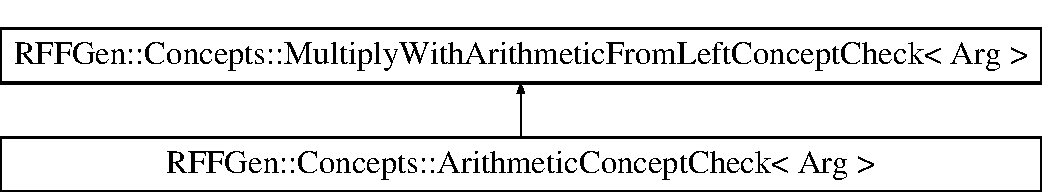
\includegraphics[height=2.000000cm]{structRFFGen_1_1Concepts_1_1MultiplyWithArithmeticFromLeftConceptCheck}
\end{center}
\end{figure}


\subsection{Detailed Description}
\subsubsection*{template$<$class Arg$>$struct R\-F\-F\-Gen\-::\-Concepts\-::\-Multiply\-With\-Arithmetic\-From\-Left\-Concept\-Check$<$ Arg $>$}

Static check if the requirements of \hyperlink{structRFFGen_1_1Concepts_1_1MultiplyWithArithmeticFromLeftConcept}{Multiply\-With\-Arithmetic\-From\-Left\-Concept} are satisfied. 


\begin{DoxyTemplParams}{Template Parameters}
{\em Arg} & type to check \\
\hline
\end{DoxyTemplParams}


The documentation for this struct was generated from the following file\-:\begin{DoxyCompactItemize}
\item 
R\-F\-F\-Gen/concept\-Check.\-hh\end{DoxyCompactItemize}

\hypertarget{classRFFGen_1_1NonSymmetricMatrixException}{\section{R\-F\-F\-Gen\-:\-:Non\-Symmetric\-Matrix\-Exception Class Reference}
\label{classRFFGen_1_1NonSymmetricMatrixException}\index{R\-F\-F\-Gen\-::\-Non\-Symmetric\-Matrix\-Exception@{R\-F\-F\-Gen\-::\-Non\-Symmetric\-Matrix\-Exception}}
}


Exception for non-\/symmetric matrices if symmetric matrices are required.  




{\ttfamily \#include $<$exceptions.\-hh$>$}

Inheritance diagram for R\-F\-F\-Gen\-:\-:Non\-Symmetric\-Matrix\-Exception\-:\begin{figure}[H]
\begin{center}
\leavevmode
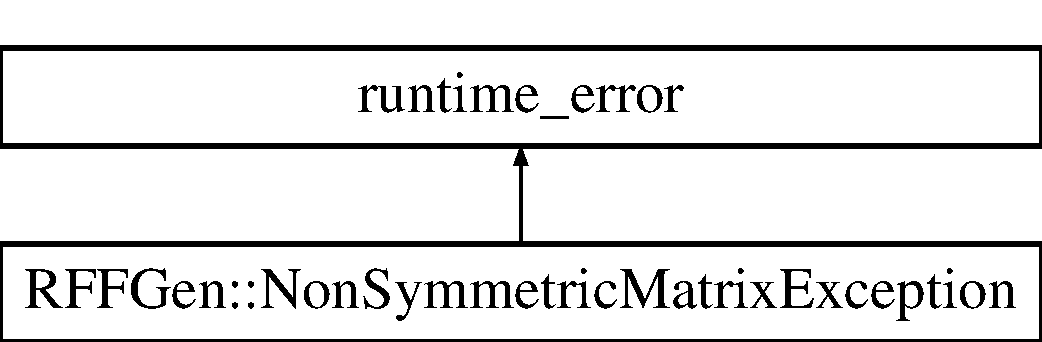
\includegraphics[height=2.000000cm]{classRFFGen_1_1NonSymmetricMatrixException}
\end{center}
\end{figure}
\subsection*{Public Member Functions}
\begin{DoxyCompactItemize}
\item 
{\footnotesize template$<$class Value , class  = std\-::enable\-\_\-if\-\_\-t$<$std\-::is\-\_\-arithmetic$<$\-Value$>$\-::value$>$$>$ }\\\hyperlink{classRFFGen_1_1NonSymmetricMatrixException_ae920b81f42489271406f48b6dc8aeaa1}{Non\-Symmetric\-Matrix\-Exception} (const std\-::string \&function, const Value \&rows, const Value \&cols, const std\-::string \&file, const int line)
\begin{DoxyCompactList}\small\item\em Constructor. \end{DoxyCompactList}\end{DoxyCompactItemize}


\subsection{Detailed Description}
Exception for non-\/symmetric matrices if symmetric matrices are required. 

\subsection{Constructor \& Destructor Documentation}
\hypertarget{classRFFGen_1_1NonSymmetricMatrixException_ae920b81f42489271406f48b6dc8aeaa1}{\index{R\-F\-F\-Gen\-::\-Non\-Symmetric\-Matrix\-Exception@{R\-F\-F\-Gen\-::\-Non\-Symmetric\-Matrix\-Exception}!Non\-Symmetric\-Matrix\-Exception@{Non\-Symmetric\-Matrix\-Exception}}
\index{Non\-Symmetric\-Matrix\-Exception@{Non\-Symmetric\-Matrix\-Exception}!RFFGen::NonSymmetricMatrixException@{R\-F\-F\-Gen\-::\-Non\-Symmetric\-Matrix\-Exception}}
\subsubsection[{Non\-Symmetric\-Matrix\-Exception}]{\setlength{\rightskip}{0pt plus 5cm}template$<$class Value , class  = std\-::enable\-\_\-if\-\_\-t$<$std\-::is\-\_\-arithmetic$<$\-Value$>$\-::value$>$$>$ R\-F\-F\-Gen\-::\-Non\-Symmetric\-Matrix\-Exception\-::\-Non\-Symmetric\-Matrix\-Exception (
\begin{DoxyParamCaption}
\item[{const std\-::string \&}]{function, }
\item[{const Value \&}]{rows, }
\item[{const Value \&}]{cols, }
\item[{const std\-::string \&}]{file, }
\item[{const int}]{line}
\end{DoxyParamCaption}
)\hspace{0.3cm}{\ttfamily [inline]}}}\label{classRFFGen_1_1NonSymmetricMatrixException_ae920b81f42489271406f48b6dc8aeaa1}


Constructor. 


\begin{DoxyParams}{Parameters}
{\em function} & name of the function throwing this exception \\
\hline
{\em rows} & number of rows of matrix \\
\hline
{\em cols} & number of columns of matrix \\
\hline
{\em file} & file containing the throwing code \\
\hline
{\em line} & line containing the throwing code \\
\hline
\end{DoxyParams}


The documentation for this class was generated from the following file\-:\begin{DoxyCompactItemize}
\item 
R\-F\-F\-Gen/\-Util/exceptions.\-hh\end{DoxyCompactItemize}

\hypertarget{structRFFGen_1_1LinearAlgebra_1_1NumberOfColumns}{\section{R\-F\-F\-Gen\-:\-:Linear\-Algebra\-:\-:Number\-Of\-Columns$<$ Matrix, class $>$ Struct Template Reference}
\label{structRFFGen_1_1LinearAlgebra_1_1NumberOfColumns}\index{R\-F\-F\-Gen\-::\-Linear\-Algebra\-::\-Number\-Of\-Columns$<$ Matrix, class $>$@{R\-F\-F\-Gen\-::\-Linear\-Algebra\-::\-Number\-Of\-Columns$<$ Matrix, class $>$}}
}


Specialize this for your matrix class. Number of columns must be provided by a static member variable called value.  




{\ttfamily \#include $<$extract\-Rows\-And\-Cols.\-hh$>$}

Inheritance diagram for R\-F\-F\-Gen\-:\-:Linear\-Algebra\-:\-:Number\-Of\-Columns$<$ Matrix, class $>$\-:\begin{figure}[H]
\begin{center}
\leavevmode
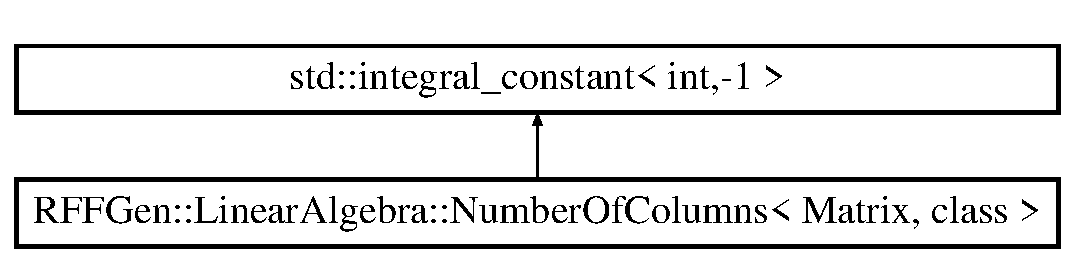
\includegraphics[height=2.000000cm]{structRFFGen_1_1LinearAlgebra_1_1NumberOfColumns}
\end{center}
\end{figure}


\subsection{Detailed Description}
\subsubsection*{template$<$class Matrix, class = Concepts\-::\-Matrix\-Concept\-Check$<$\-Matrix$>$$>$struct R\-F\-F\-Gen\-::\-Linear\-Algebra\-::\-Number\-Of\-Columns$<$ Matrix, class $>$}

Specialize this for your matrix class. Number of columns must be provided by a static member variable called value. 

The documentation for this struct was generated from the following file\-:\begin{DoxyCompactItemize}
\item 
R\-F\-F\-Gen/\-Linear\-Algebra/extract\-Rows\-And\-Cols.\-hh\end{DoxyCompactItemize}

\hypertarget{structRFFGen_1_1LinearAlgebra_1_1NumberOfColumns_3_01Matrix_3_01n_00_01m_01_4_00_01MatrixConceptCheck_01_4}{\section{R\-F\-F\-Gen\-:\-:Linear\-Algebra\-:\-:Number\-Of\-Columns$<$ Matrix$<$ n, m $>$, Matrix\-Concept\-Check $>$ Struct Template Reference}
\label{structRFFGen_1_1LinearAlgebra_1_1NumberOfColumns_3_01Matrix_3_01n_00_01m_01_4_00_01MatrixConceptCheck_01_4}\index{R\-F\-F\-Gen\-::\-Linear\-Algebra\-::\-Number\-Of\-Columns$<$ Matrix$<$ n, m $>$, Matrix\-Concept\-Check $>$@{R\-F\-F\-Gen\-::\-Linear\-Algebra\-::\-Number\-Of\-Columns$<$ Matrix$<$ n, m $>$, Matrix\-Concept\-Check $>$}}
}


Specialization for matrices.  




{\ttfamily \#include $<$extract\-Rows\-And\-Cols.\-hh$>$}

Inheritance diagram for R\-F\-F\-Gen\-:\-:Linear\-Algebra\-:\-:Number\-Of\-Columns$<$ Matrix$<$ n, m $>$, Matrix\-Concept\-Check $>$\-:\begin{figure}[H]
\begin{center}
\leavevmode
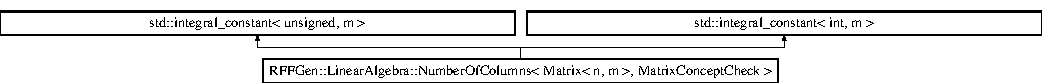
\includegraphics[height=1.117764cm]{structRFFGen_1_1LinearAlgebra_1_1NumberOfColumns_3_01Matrix_3_01n_00_01m_01_4_00_01MatrixConceptCheck_01_4}
\end{center}
\end{figure}


\subsection{Detailed Description}
\subsubsection*{template$<$template$<$ int, int $>$ class Matrix, int n, int m, class Matrix\-Concept\-Check$>$struct R\-F\-F\-Gen\-::\-Linear\-Algebra\-::\-Number\-Of\-Columns$<$ Matrix$<$ n, m $>$, Matrix\-Concept\-Check $>$}

Specialization for matrices. 

The documentation for this struct was generated from the following file\-:\begin{DoxyCompactItemize}
\item 
R\-F\-F\-Gen/\-Linear\-Algebra/extract\-Rows\-And\-Cols.\-hh\end{DoxyCompactItemize}

\hypertarget{structRFFGen_1_1LinearAlgebra_1_1NumberOfColumns_3_01Matrix_3_01T_00_01n_00_01m_01_4_00_01MatrixConceptCheck_01_4}{\section{R\-F\-F\-Gen\-:\-:Linear\-Algebra\-:\-:Number\-Of\-Columns$<$ Matrix$<$ T, n, m $>$, Matrix\-Concept\-Check $>$ Struct Template Reference}
\label{structRFFGen_1_1LinearAlgebra_1_1NumberOfColumns_3_01Matrix_3_01T_00_01n_00_01m_01_4_00_01MatrixConceptCheck_01_4}\index{R\-F\-F\-Gen\-::\-Linear\-Algebra\-::\-Number\-Of\-Columns$<$ Matrix$<$ T, n, m $>$, Matrix\-Concept\-Check $>$@{R\-F\-F\-Gen\-::\-Linear\-Algebra\-::\-Number\-Of\-Columns$<$ Matrix$<$ T, n, m $>$, Matrix\-Concept\-Check $>$}}
}


Specialization for matrices.  




{\ttfamily \#include $<$extract\-Rows\-And\-Cols.\-hh$>$}

Inheritance diagram for R\-F\-F\-Gen\-:\-:Linear\-Algebra\-:\-:Number\-Of\-Columns$<$ Matrix$<$ T, n, m $>$, Matrix\-Concept\-Check $>$\-:\begin{figure}[H]
\begin{center}
\leavevmode
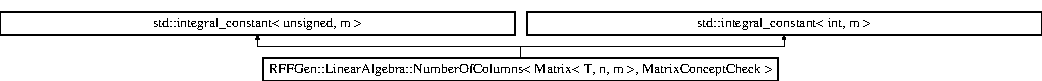
\includegraphics[height=1.083172cm]{structRFFGen_1_1LinearAlgebra_1_1NumberOfColumns_3_01Matrix_3_01T_00_01n_00_01m_01_4_00_01MatrixConceptCheck_01_4}
\end{center}
\end{figure}


\subsection{Detailed Description}
\subsubsection*{template$<$template$<$ class, int, int $>$ class Matrix, class T, int n, int m, class Matrix\-Concept\-Check$>$struct R\-F\-F\-Gen\-::\-Linear\-Algebra\-::\-Number\-Of\-Columns$<$ Matrix$<$ T, n, m $>$, Matrix\-Concept\-Check $>$}

Specialization for matrices. 

The documentation for this struct was generated from the following file\-:\begin{DoxyCompactItemize}
\item 
R\-F\-F\-Gen/\-Linear\-Algebra/extract\-Rows\-And\-Cols.\-hh\end{DoxyCompactItemize}

\hypertarget{structRFFGen_1_1LinearAlgebra_1_1NumberOfRows}{\section{R\-F\-F\-Gen\-:\-:Linear\-Algebra\-:\-:Number\-Of\-Rows$<$ Matrix, class $>$ Struct Template Reference}
\label{structRFFGen_1_1LinearAlgebra_1_1NumberOfRows}\index{R\-F\-F\-Gen\-::\-Linear\-Algebra\-::\-Number\-Of\-Rows$<$ Matrix, class $>$@{R\-F\-F\-Gen\-::\-Linear\-Algebra\-::\-Number\-Of\-Rows$<$ Matrix, class $>$}}
}


Specialize this for your matrix class. Number of rows must be provided by a static member variable called value.  




{\ttfamily \#include $<$extract\-Rows\-And\-Cols.\-hh$>$}

Inheritance diagram for R\-F\-F\-Gen\-:\-:Linear\-Algebra\-:\-:Number\-Of\-Rows$<$ Matrix, class $>$\-:\begin{figure}[H]
\begin{center}
\leavevmode
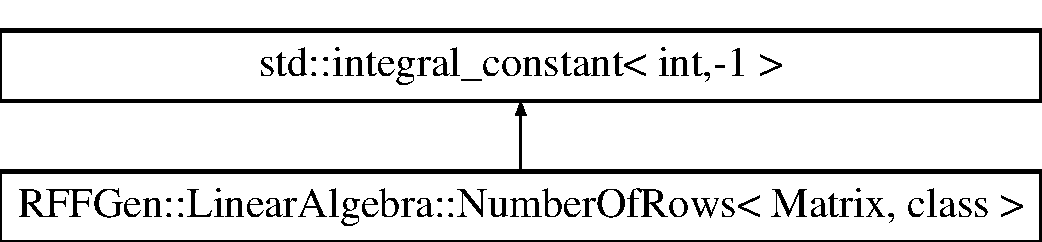
\includegraphics[height=2.000000cm]{structRFFGen_1_1LinearAlgebra_1_1NumberOfRows}
\end{center}
\end{figure}


\subsection{Detailed Description}
\subsubsection*{template$<$class Matrix, class = Concepts\-::\-Matrix\-Concept\-Check$<$\-Matrix$>$$>$struct R\-F\-F\-Gen\-::\-Linear\-Algebra\-::\-Number\-Of\-Rows$<$ Matrix, class $>$}

Specialize this for your matrix class. Number of rows must be provided by a static member variable called value. 

The documentation for this struct was generated from the following file\-:\begin{DoxyCompactItemize}
\item 
R\-F\-F\-Gen/\-Linear\-Algebra/extract\-Rows\-And\-Cols.\-hh\end{DoxyCompactItemize}

\hypertarget{structRFFGen_1_1LinearAlgebra_1_1NumberOfRows_3_01Matrix_3_01n_00_01m_01_4_00_01MatrixConceptCheck_01_4}{\section{R\-F\-F\-Gen\-:\-:Linear\-Algebra\-:\-:Number\-Of\-Rows$<$ Matrix$<$ n, m $>$, Matrix\-Concept\-Check $>$ Struct Template Reference}
\label{structRFFGen_1_1LinearAlgebra_1_1NumberOfRows_3_01Matrix_3_01n_00_01m_01_4_00_01MatrixConceptCheck_01_4}\index{R\-F\-F\-Gen\-::\-Linear\-Algebra\-::\-Number\-Of\-Rows$<$ Matrix$<$ n, m $>$, Matrix\-Concept\-Check $>$@{R\-F\-F\-Gen\-::\-Linear\-Algebra\-::\-Number\-Of\-Rows$<$ Matrix$<$ n, m $>$, Matrix\-Concept\-Check $>$}}
}


Specialization for matrices.  




{\ttfamily \#include $<$extract\-Rows\-And\-Cols.\-hh$>$}

Inheritance diagram for R\-F\-F\-Gen\-:\-:Linear\-Algebra\-:\-:Number\-Of\-Rows$<$ Matrix$<$ n, m $>$, Matrix\-Concept\-Check $>$\-:\begin{figure}[H]
\begin{center}
\leavevmode
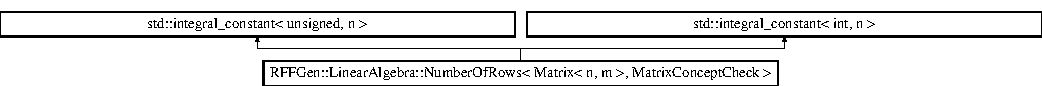
\includegraphics[height=1.159420cm]{structRFFGen_1_1LinearAlgebra_1_1NumberOfRows_3_01Matrix_3_01n_00_01m_01_4_00_01MatrixConceptCheck_01_4}
\end{center}
\end{figure}


\subsection{Detailed Description}
\subsubsection*{template$<$template$<$ int, int $>$ class Matrix, int n, int m, class Matrix\-Concept\-Check$>$struct R\-F\-F\-Gen\-::\-Linear\-Algebra\-::\-Number\-Of\-Rows$<$ Matrix$<$ n, m $>$, Matrix\-Concept\-Check $>$}

Specialization for matrices. 

The documentation for this struct was generated from the following file\-:\begin{DoxyCompactItemize}
\item 
R\-F\-F\-Gen/\-Linear\-Algebra/extract\-Rows\-And\-Cols.\-hh\end{DoxyCompactItemize}

\hypertarget{structRFFGen_1_1LinearAlgebra_1_1NumberOfRows_3_01Matrix_3_01T_00_01n_00_01m_01_4_00_01MatrixConceptCheck_01_4}{\section{R\-F\-F\-Gen\-:\-:Linear\-Algebra\-:\-:Number\-Of\-Rows$<$ Matrix$<$ T, n, m $>$, Matrix\-Concept\-Check $>$ Struct Template Reference}
\label{structRFFGen_1_1LinearAlgebra_1_1NumberOfRows_3_01Matrix_3_01T_00_01n_00_01m_01_4_00_01MatrixConceptCheck_01_4}\index{R\-F\-F\-Gen\-::\-Linear\-Algebra\-::\-Number\-Of\-Rows$<$ Matrix$<$ T, n, m $>$, Matrix\-Concept\-Check $>$@{R\-F\-F\-Gen\-::\-Linear\-Algebra\-::\-Number\-Of\-Rows$<$ Matrix$<$ T, n, m $>$, Matrix\-Concept\-Check $>$}}
}


Specialization for matrices.  




{\ttfamily \#include $<$extract\-Rows\-And\-Cols.\-hh$>$}

Inheritance diagram for R\-F\-F\-Gen\-:\-:Linear\-Algebra\-:\-:Number\-Of\-Rows$<$ Matrix$<$ T, n, m $>$, Matrix\-Concept\-Check $>$\-:\begin{figure}[H]
\begin{center}
\leavevmode
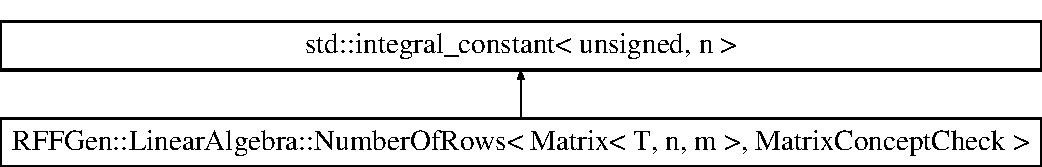
\includegraphics[height=2.000000cm]{structRFFGen_1_1LinearAlgebra_1_1NumberOfRows_3_01Matrix_3_01T_00_01n_00_01m_01_4_00_01MatrixConceptCheck_01_4}
\end{center}
\end{figure}


\subsection{Detailed Description}
\subsubsection*{template$<$template$<$ class, unsigned, unsigned $>$ class Matrix, class T, unsigned n, unsigned m, class Matrix\-Concept\-Check$>$struct R\-F\-F\-Gen\-::\-Linear\-Algebra\-::\-Number\-Of\-Rows$<$ Matrix$<$ T, n, m $>$, Matrix\-Concept\-Check $>$}

Specialization for matrices. 

The documentation for this struct was generated from the following file\-:\begin{DoxyCompactItemize}
\item 
R\-F\-F\-Gen/\-Linear\-Algebra/extract\-Rows\-And\-Cols.\-hh\end{DoxyCompactItemize}

\hypertarget{structRFFGen_1_1LinearAlgebra_1_1NumberOfRows_3_01Vector_3_01n_01_4_00_01MatrixConceptCheck_01_4}{\section{R\-F\-F\-Gen\-:\-:Linear\-Algebra\-:\-:Number\-Of\-Rows$<$ Vector$<$ n $>$, Matrix\-Concept\-Check $>$ Struct Template Reference}
\label{structRFFGen_1_1LinearAlgebra_1_1NumberOfRows_3_01Vector_3_01n_01_4_00_01MatrixConceptCheck_01_4}\index{R\-F\-F\-Gen\-::\-Linear\-Algebra\-::\-Number\-Of\-Rows$<$ Vector$<$ n $>$, Matrix\-Concept\-Check $>$@{R\-F\-F\-Gen\-::\-Linear\-Algebra\-::\-Number\-Of\-Rows$<$ Vector$<$ n $>$, Matrix\-Concept\-Check $>$}}
}


Specialization for vectors.  




{\ttfamily \#include $<$extract\-Rows\-And\-Cols.\-hh$>$}

Inheritance diagram for R\-F\-F\-Gen\-:\-:Linear\-Algebra\-:\-:Number\-Of\-Rows$<$ Vector$<$ n $>$, Matrix\-Concept\-Check $>$\-:\begin{figure}[H]
\begin{center}
\leavevmode
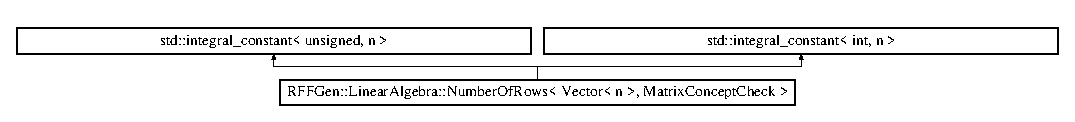
\includegraphics[height=1.196581cm]{structRFFGen_1_1LinearAlgebra_1_1NumberOfRows_3_01Vector_3_01n_01_4_00_01MatrixConceptCheck_01_4}
\end{center}
\end{figure}


\subsection{Detailed Description}
\subsubsection*{template$<$template$<$ int $>$ class Vector, int n, class Matrix\-Concept\-Check$>$struct R\-F\-F\-Gen\-::\-Linear\-Algebra\-::\-Number\-Of\-Rows$<$ Vector$<$ n $>$, Matrix\-Concept\-Check $>$}

Specialization for vectors. 

The documentation for this struct was generated from the following file\-:\begin{DoxyCompactItemize}
\item 
R\-F\-F\-Gen/\-Linear\-Algebra/extract\-Rows\-And\-Cols.\-hh\end{DoxyCompactItemize}

\hypertarget{structRFFGen_1_1LinearAlgebra_1_1NumberOfRows_3_01Vector_3_01T_00_01n_01_4_00_01MatrixConceptCheck_01_4}{\section{R\-F\-F\-Gen\-:\-:Linear\-Algebra\-:\-:Number\-Of\-Rows$<$ Vector$<$ T, n $>$, Matrix\-Concept\-Check $>$ Struct Template Reference}
\label{structRFFGen_1_1LinearAlgebra_1_1NumberOfRows_3_01Vector_3_01T_00_01n_01_4_00_01MatrixConceptCheck_01_4}\index{R\-F\-F\-Gen\-::\-Linear\-Algebra\-::\-Number\-Of\-Rows$<$ Vector$<$ T, n $>$, Matrix\-Concept\-Check $>$@{R\-F\-F\-Gen\-::\-Linear\-Algebra\-::\-Number\-Of\-Rows$<$ Vector$<$ T, n $>$, Matrix\-Concept\-Check $>$}}
}


Specialization for vectors.  




{\ttfamily \#include $<$extract\-Rows\-And\-Cols.\-hh$>$}

Inheritance diagram for R\-F\-F\-Gen\-:\-:Linear\-Algebra\-:\-:Number\-Of\-Rows$<$ Vector$<$ T, n $>$, Matrix\-Concept\-Check $>$\-:\begin{figure}[H]
\begin{center}
\leavevmode
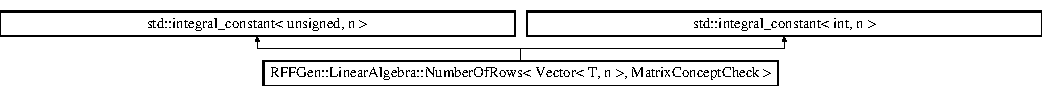
\includegraphics[height=1.157025cm]{structRFFGen_1_1LinearAlgebra_1_1NumberOfRows_3_01Vector_3_01T_00_01n_01_4_00_01MatrixConceptCheck_01_4}
\end{center}
\end{figure}


\subsection{Detailed Description}
\subsubsection*{template$<$template$<$ class, int $>$ class Vector, class T, int n, class Matrix\-Concept\-Check$>$struct R\-F\-F\-Gen\-::\-Linear\-Algebra\-::\-Number\-Of\-Rows$<$ Vector$<$ T, n $>$, Matrix\-Concept\-Check $>$}

Specialization for vectors. 

The documentation for this struct was generated from the following file\-:\begin{DoxyCompactItemize}
\item 
R\-F\-F\-Gen/\-Linear\-Algebra/extract\-Rows\-And\-Cols.\-hh\end{DoxyCompactItemize}

\hypertarget{classRFFGen_1_1OutOfDomainException}{\section{R\-F\-F\-Gen\-:\-:Out\-Of\-Domain\-Exception Class Reference}
\label{classRFFGen_1_1OutOfDomainException}\index{R\-F\-F\-Gen\-::\-Out\-Of\-Domain\-Exception@{R\-F\-F\-Gen\-::\-Out\-Of\-Domain\-Exception}}
}


Exception for scalar function arguments that are outside the domain of the function.  




{\ttfamily \#include $<$exceptions.\-hh$>$}

Inheritance diagram for R\-F\-F\-Gen\-:\-:Out\-Of\-Domain\-Exception\-:\begin{figure}[H]
\begin{center}
\leavevmode
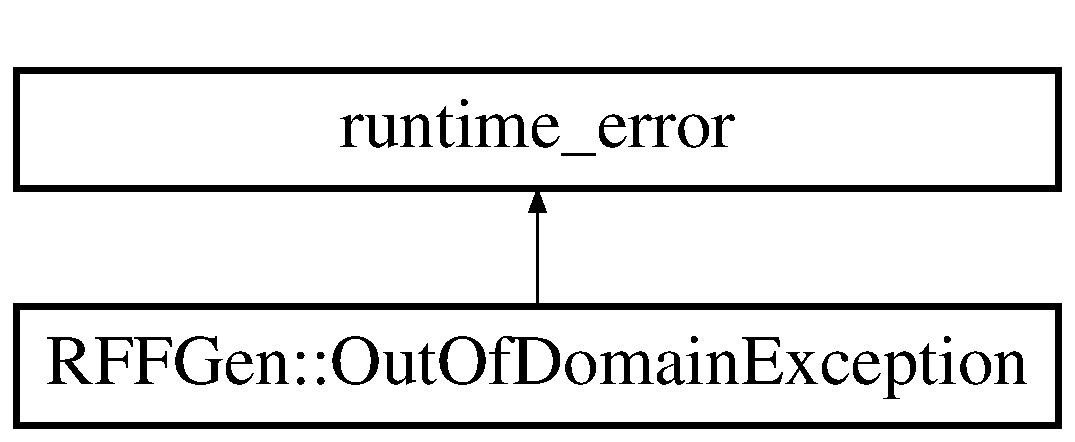
\includegraphics[height=2.000000cm]{classRFFGen_1_1OutOfDomainException}
\end{center}
\end{figure}
\subsection*{Public Member Functions}
\begin{DoxyCompactItemize}
\item 
{\footnotesize template$<$class Value , class  = std\-::enable\-\_\-if\-\_\-t$<$std\-::is\-\_\-arithmetic$<$\-Value$>$\-::value$>$$>$ }\\\hyperlink{classRFFGen_1_1OutOfDomainException_a3152ef040f15248bf49b7f4734ad4734}{Out\-Of\-Domain\-Exception} (const std\-::string \&function, const std\-::string \&range, const Value \&value, const std\-::string \&file, const int line)
\begin{DoxyCompactList}\small\item\em Constructor. \end{DoxyCompactList}\end{DoxyCompactItemize}


\subsection{Detailed Description}
Exception for scalar function arguments that are outside the domain of the function. 

Example\-: 
\begin{DoxyCode}
\textcolor{keywordflow}{if}( x < 0 )
  \textcolor{keywordflow}{throw} \hyperlink{classRFFGen_1_1OutOfDomainException_a3152ef040f15248bf49b7f4734ad4734}{OutOfDomainException}(\textcolor{stringliteral}{"[0,inf["},\textcolor{stringliteral}{"Sqrt"} x,\_\_FILE\_\_,\_\_LINE\_\_);
\end{DoxyCode}
 

\subsection{Constructor \& Destructor Documentation}
\hypertarget{classRFFGen_1_1OutOfDomainException_a3152ef040f15248bf49b7f4734ad4734}{\index{R\-F\-F\-Gen\-::\-Out\-Of\-Domain\-Exception@{R\-F\-F\-Gen\-::\-Out\-Of\-Domain\-Exception}!Out\-Of\-Domain\-Exception@{Out\-Of\-Domain\-Exception}}
\index{Out\-Of\-Domain\-Exception@{Out\-Of\-Domain\-Exception}!RFFGen::OutOfDomainException@{R\-F\-F\-Gen\-::\-Out\-Of\-Domain\-Exception}}
\subsubsection[{Out\-Of\-Domain\-Exception}]{\setlength{\rightskip}{0pt plus 5cm}template$<$class Value , class  = std\-::enable\-\_\-if\-\_\-t$<$std\-::is\-\_\-arithmetic$<$\-Value$>$\-::value$>$$>$ R\-F\-F\-Gen\-::\-Out\-Of\-Domain\-Exception\-::\-Out\-Of\-Domain\-Exception (
\begin{DoxyParamCaption}
\item[{const std\-::string \&}]{function, }
\item[{const std\-::string \&}]{range, }
\item[{const Value \&}]{value, }
\item[{const std\-::string \&}]{file, }
\item[{const int}]{line}
\end{DoxyParamCaption}
)\hspace{0.3cm}{\ttfamily [inline]}}}\label{classRFFGen_1_1OutOfDomainException_a3152ef040f15248bf49b7f4734ad4734}


Constructor. 


\begin{DoxyParams}{Parameters}
{\em range} & std\-::string that contains the mathematical expression for the valid range \\
\hline
{\em function} & name of the function throwing this exception \\
\hline
{\em value} & value outside range \\
\hline
{\em file} & file containing the throwing code \\
\hline
{\em line} & line containing the throwing code \\
\hline
\end{DoxyParams}


The documentation for this class was generated from the following file\-:\begin{DoxyCompactItemize}
\item 
R\-F\-F\-Gen/\-Util/exceptions.\-hh\end{DoxyCompactItemize}

\hypertarget{structRFFGen_1_1CMath_1_1Pow}{\section{R\-F\-F\-Gen\-:\-:C\-Math\-:\-:Pow$<$ dividend, divisor $>$ Struct Template Reference}
\label{structRFFGen_1_1CMath_1_1Pow}\index{R\-F\-F\-Gen\-::\-C\-Math\-::\-Pow$<$ dividend, divisor $>$@{R\-F\-F\-Gen\-::\-C\-Math\-::\-Pow$<$ dividend, divisor $>$}}
}


Power function with rational exponent $ k = \frac{dividend}{divisor} $ including first three derivatives.  




{\ttfamily \#include $<$pow.\-hh$>$}

Inheritance diagram for R\-F\-F\-Gen\-:\-:C\-Math\-:\-:Pow$<$ dividend, divisor $>$\-:\begin{figure}[H]
\begin{center}
\leavevmode
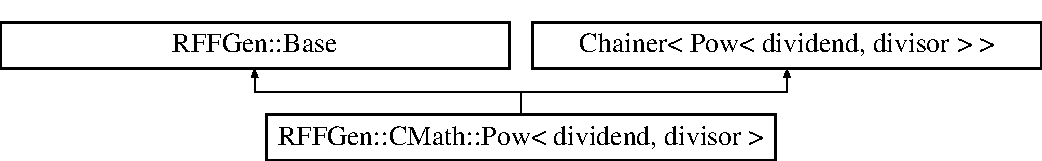
\includegraphics[height=2.000000cm]{structRFFGen_1_1CMath_1_1Pow}
\end{center}
\end{figure}
\subsection*{Public Member Functions}
\begin{DoxyCompactItemize}
\item 
\hyperlink{structRFFGen_1_1CMath_1_1Pow_a6b1f2413fa8ce7ae9064ee7e948da7eb}{Pow} (double x=1)
\begin{DoxyCompactList}\small\item\em Constructor. \end{DoxyCompactList}\item 
\hypertarget{structRFFGen_1_1CMath_1_1Pow_aabed9b037ca197924bf683c04d175449}{void \hyperlink{structRFFGen_1_1CMath_1_1Pow_aabed9b037ca197924bf683c04d175449}{update} (double x)}\label{structRFFGen_1_1CMath_1_1Pow_aabed9b037ca197924bf683c04d175449}

\begin{DoxyCompactList}\small\item\em Reset point of evaluation. \end{DoxyCompactList}\item 
\hypertarget{structRFFGen_1_1CMath_1_1Pow_a62c4da4570b12af2e56861600f9ce420}{double \hyperlink{structRFFGen_1_1CMath_1_1Pow_a62c4da4570b12af2e56861600f9ce420}{d0} () const noexcept}\label{structRFFGen_1_1CMath_1_1Pow_a62c4da4570b12af2e56861600f9ce420}

\begin{DoxyCompactList}\small\item\em Function value. \end{DoxyCompactList}\item 
\hypertarget{structRFFGen_1_1CMath_1_1Pow_af2d6a3bee0ab59865f309e5a27f0bf9f}{{\footnotesize template$<$int  = -\/1$>$ }\\double \hyperlink{structRFFGen_1_1CMath_1_1Pow_af2d6a3bee0ab59865f309e5a27f0bf9f}{d1} (double dx=1.) const }\label{structRFFGen_1_1CMath_1_1Pow_af2d6a3bee0ab59865f309e5a27f0bf9f}

\begin{DoxyCompactList}\small\item\em First (directional) derivative. \end{DoxyCompactList}\item 
\hypertarget{structRFFGen_1_1CMath_1_1Pow_ac733ea45c6cfccdc11e7c4206c4641ab}{{\footnotesize template$<$int  = -\/1, int  = -\/1$>$ }\\double \hyperlink{structRFFGen_1_1CMath_1_1Pow_ac733ea45c6cfccdc11e7c4206c4641ab}{d2} (double dx=1., double dy=1.) const }\label{structRFFGen_1_1CMath_1_1Pow_ac733ea45c6cfccdc11e7c4206c4641ab}

\begin{DoxyCompactList}\small\item\em Second (directinal) derivative. \end{DoxyCompactList}\item 
\hypertarget{structRFFGen_1_1CMath_1_1Pow_aa98931e90793bd54740c056dde37c9d8}{{\footnotesize template$<$int  = -\/1, int  = -\/1, int  = -\/1$>$ }\\double \hyperlink{structRFFGen_1_1CMath_1_1Pow_aa98931e90793bd54740c056dde37c9d8}{d3} (double dx=1., double dy=1., double dz=1.) const }\label{structRFFGen_1_1CMath_1_1Pow_aa98931e90793bd54740c056dde37c9d8}

\begin{DoxyCompactList}\small\item\em Third (directional) derivative. \end{DoxyCompactList}\end{DoxyCompactItemize}


\subsection{Detailed Description}
\subsubsection*{template$<$int dividend, int divisor = 1$>$struct R\-F\-F\-Gen\-::\-C\-Math\-::\-Pow$<$ dividend, divisor $>$}

Power function with rational exponent $ k = \frac{dividend}{divisor} $ including first three derivatives. 

For scalar functions directional derivatives are less interesting. Incorporating this function as building block for more complex functions requires directional derivatives. These occur during applications of the chain rule. For the cases $k=-1$ and $k=2$ specializations are used that avoid the use of std\-::pow. 

\subsection{Constructor \& Destructor Documentation}
\hypertarget{structRFFGen_1_1CMath_1_1Pow_a6b1f2413fa8ce7ae9064ee7e948da7eb}{\index{R\-F\-F\-Gen\-::\-C\-Math\-::\-Pow@{R\-F\-F\-Gen\-::\-C\-Math\-::\-Pow}!Pow@{Pow}}
\index{Pow@{Pow}!RFFGen::CMath::Pow@{R\-F\-F\-Gen\-::\-C\-Math\-::\-Pow}}
\subsubsection[{Pow}]{\setlength{\rightskip}{0pt plus 5cm}template$<$int dividend, int divisor = 1$>$ {\bf R\-F\-F\-Gen\-::\-C\-Math\-::\-Pow}$<$ dividend, divisor $>$\-::{\bf Pow} (
\begin{DoxyParamCaption}
\item[{double}]{x = {\ttfamily 1}}
\end{DoxyParamCaption}
)\hspace{0.3cm}{\ttfamily [inline]}, {\ttfamily [explicit]}}}\label{structRFFGen_1_1CMath_1_1Pow_a6b1f2413fa8ce7ae9064ee7e948da7eb}


Constructor. 


\begin{DoxyParams}{Parameters}
{\em x} & point of evaluation \\
\hline
\end{DoxyParams}


The documentation for this struct was generated from the following file\-:\begin{DoxyCompactItemize}
\item 
R\-F\-F\-Gen/\-C\-Math/pow.\-hh\end{DoxyCompactItemize}

\hypertarget{structRFFGen_1_1MathematicalOperations_1_1Product}{\section{R\-F\-F\-Gen\-:\-:Mathematical\-Operations\-:\-:Product$<$ F, G, class, class $>$ Struct Template Reference}
\label{structRFFGen_1_1MathematicalOperations_1_1Product}\index{R\-F\-F\-Gen\-::\-Mathematical\-Operations\-::\-Product$<$ F, G, class, class $>$@{R\-F\-F\-Gen\-::\-Mathematical\-Operations\-::\-Product$<$ F, G, class, class $>$}}
}


Product $fg$ of functions of type F and G (F and G must satisfy the requirements of \hyperlink{structRFFGen_1_1Concepts_1_1FunctionConcept}{Concepts\-::\-Function\-Concept}).  




{\ttfamily \#include $<$product.\-hh$>$}

Inheritance diagram for R\-F\-F\-Gen\-:\-:Mathematical\-Operations\-:\-:Product$<$ F, G, class, class $>$\-:\begin{figure}[H]
\begin{center}
\leavevmode
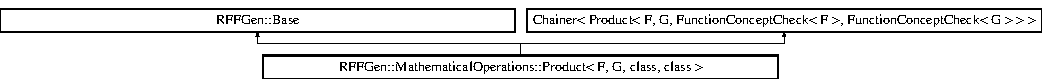
\includegraphics[height=1.056604cm]{structRFFGen_1_1MathematicalOperations_1_1Product}
\end{center}
\end{figure}
\subsection*{Public Member Functions}
\begin{DoxyCompactItemize}
\item 
\hypertarget{structRFFGen_1_1MathematicalOperations_1_1Product_a8f90fefe7c771b6dcb3b714c85be41fa}{\hyperlink{structRFFGen_1_1MathematicalOperations_1_1Product_a8f90fefe7c771b6dcb3b714c85be41fa}{Product} ()=default}\label{structRFFGen_1_1MathematicalOperations_1_1Product_a8f90fefe7c771b6dcb3b714c85be41fa}

\begin{DoxyCompactList}\small\item\em Default constructor. May leave member variables uninitialized! Call update before using evaluation. \end{DoxyCompactList}\item 
{\footnotesize template$<$class Init\-F , class Init\-G $>$ }\\\hyperlink{structRFFGen_1_1MathematicalOperations_1_1Product_aaa4efed57c0ed72f39d363c88fa04da0}{Product} (const Init\-F \&f\-\_\-, const Init\-G \&g\-\_\-)
\begin{DoxyCompactList}\small\item\em Constructor passing arguments to function constructors. \end{DoxyCompactList}\item 
\hypertarget{structRFFGen_1_1MathematicalOperations_1_1Product_a4cfbb3c643899bb7e3468587d9800a26}{{\footnotesize template$<$class Arg $>$ }\\void \hyperlink{structRFFGen_1_1MathematicalOperations_1_1Product_a4cfbb3c643899bb7e3468587d9800a26}{update} (Arg const \&x)}\label{structRFFGen_1_1MathematicalOperations_1_1Product_a4cfbb3c643899bb7e3468587d9800a26}

\begin{DoxyCompactList}\small\item\em Reset point of evaluation. \end{DoxyCompactList}\item 
\hypertarget{structRFFGen_1_1MathematicalOperations_1_1Product_ade58e75205d33ba03780b934e4b379c3}{{\footnotesize template$<$int index, class Arg $>$ }\\void \hyperlink{structRFFGen_1_1MathematicalOperations_1_1Product_ade58e75205d33ba03780b934e4b379c3}{update\-Variable} (const Arg \&x)}\label{structRFFGen_1_1MathematicalOperations_1_1Product_ade58e75205d33ba03780b934e4b379c3}

\begin{DoxyCompactList}\small\item\em Propagate call to \hyperlink{structRFFGen_1_1MathematicalOperations_1_1Product_ade58e75205d33ba03780b934e4b379c3}{update\-Variable()} to f and g. \end{DoxyCompactList}\item 
\hypertarget{structRFFGen_1_1MathematicalOperations_1_1Product_a7418270e2b7e568975254ec0feddda57}{auto \hyperlink{structRFFGen_1_1MathematicalOperations_1_1Product_a7418270e2b7e568975254ec0feddda57}{d0} () const noexcept}\label{structRFFGen_1_1MathematicalOperations_1_1Product_a7418270e2b7e568975254ec0feddda57}

\begin{DoxyCompactList}\small\item\em Function value. \end{DoxyCompactList}\item 
{\footnotesize template$<$int id, class Arg , class Indexed\-Arg  = Indexed\-Type$<$\-Arg,id$>$, class  = std\-::enable\-\_\-if\-\_\-t$<$ D1\-Type$<$\-Indexed\-Arg$>$\-::present $>$$>$ }\\auto \hyperlink{structRFFGen_1_1MathematicalOperations_1_1Product_a931ee710bfb4efa05a2dcc3182b450c5}{d1} (Arg const \&dx) const 
\begin{DoxyCompactList}\small\item\em First directional derivative. \end{DoxyCompactList}\item 
{\footnotesize template$<$int idx, int idy, class Arg\-X , class Arg\-Y , class Indexed\-Arg\-X  = Indexed\-Type$<$\-Arg\-X,idx$>$, class Indexed\-Arg\-Y  = Indexed\-Type$<$\-Arg\-Y,idy$>$, class  = std\-::enable\-\_\-if\-\_\-t$<$ D2\-Type$<$\-Indexed\-Arg\-X,\-Indexed\-Arg\-Y$>$\-::present $>$$>$ }\\auto \hyperlink{structRFFGen_1_1MathematicalOperations_1_1Product_a467d662ec3a47475a83d2e3c8ed002e3}{d2} (Arg\-X const \&dx, Arg\-Y const \&dy) const 
\begin{DoxyCompactList}\small\item\em Second directional derivative. \end{DoxyCompactList}\item 
{\footnotesize template$<$int idx, int idy, int idz, class Arg\-X , class Arg\-Y , class Arg\-Z , class Indexed\-Arg\-X  = Indexed\-Type$<$\-Arg\-X,idx$>$, class Indexed\-Arg\-Y  = Indexed\-Type$<$\-Arg\-Y,idy$>$, class Indexed\-Arg\-Z  = Indexed\-Type$<$\-Arg\-Z,idz$>$, class  = std\-::enable\-\_\-if\-\_\-t$<$ D3\-Type$<$\-Indexed\-Arg\-X,\-Indexed\-Arg\-Y,\-Indexed\-Arg\-Z$>$\-::present $>$$>$ }\\auto \hyperlink{structRFFGen_1_1MathematicalOperations_1_1Product_a155fb5653aeaf258dc4e23e8ccb734b3}{d3} (Arg\-X const \&dx, Arg\-Y const \&dy, Arg\-Z const \&dz) const 
\begin{DoxyCompactList}\small\item\em Third directional derivative. \end{DoxyCompactList}\end{DoxyCompactItemize}


\subsection{Detailed Description}
\subsubsection*{template$<$class F, class G, class = Function\-Concept\-Check$<$\-F$>$, class = Function\-Concept\-Check$<$\-G$>$$>$struct R\-F\-F\-Gen\-::\-Mathematical\-Operations\-::\-Product$<$ F, G, class, class $>$}

Product $fg$ of functions of type F and G (F and G must satisfy the requirements of \hyperlink{structRFFGen_1_1Concepts_1_1FunctionConcept}{Concepts\-::\-Function\-Concept}). 

\subsection{Constructor \& Destructor Documentation}
\hypertarget{structRFFGen_1_1MathematicalOperations_1_1Product_aaa4efed57c0ed72f39d363c88fa04da0}{\index{R\-F\-F\-Gen\-::\-Mathematical\-Operations\-::\-Product@{R\-F\-F\-Gen\-::\-Mathematical\-Operations\-::\-Product}!Product@{Product}}
\index{Product@{Product}!RFFGen::MathematicalOperations::Product@{R\-F\-F\-Gen\-::\-Mathematical\-Operations\-::\-Product}}
\subsubsection[{Product}]{\setlength{\rightskip}{0pt plus 5cm}template$<$class F , class G , class  = Function\-Concept\-Check$<$\-F$>$, class  = Function\-Concept\-Check$<$\-G$>$$>$ template$<$class Init\-F , class Init\-G $>$ {\bf R\-F\-F\-Gen\-::\-Mathematical\-Operations\-::\-Product}$<$ F, G, class, class $>$\-::{\bf Product} (
\begin{DoxyParamCaption}
\item[{const Init\-F \&}]{f\-\_\-, }
\item[{const Init\-G \&}]{g\-\_\-}
\end{DoxyParamCaption}
)\hspace{0.3cm}{\ttfamily [inline]}}}\label{structRFFGen_1_1MathematicalOperations_1_1Product_aaa4efed57c0ed72f39d363c88fa04da0}


Constructor passing arguments to function constructors. 


\begin{DoxyParams}{Parameters}
{\em f\-\_\-} & input for constructor of left side of product \\
\hline
{\em g\-\_\-} & input for constructor of right side of product \\
\hline
\end{DoxyParams}


\subsection{Member Function Documentation}
\hypertarget{structRFFGen_1_1MathematicalOperations_1_1Product_a931ee710bfb4efa05a2dcc3182b450c5}{\index{R\-F\-F\-Gen\-::\-Mathematical\-Operations\-::\-Product@{R\-F\-F\-Gen\-::\-Mathematical\-Operations\-::\-Product}!d1@{d1}}
\index{d1@{d1}!RFFGen::MathematicalOperations::Product@{R\-F\-F\-Gen\-::\-Mathematical\-Operations\-::\-Product}}
\subsubsection[{d1}]{\setlength{\rightskip}{0pt plus 5cm}template$<$class F , class G , class  = Function\-Concept\-Check$<$\-F$>$, class  = Function\-Concept\-Check$<$\-G$>$$>$ template$<$int id, class Arg , class Indexed\-Arg  = Indexed\-Type$<$\-Arg,id$>$, class  = std\-::enable\-\_\-if\-\_\-t$<$ D1\-Type$<$\-Indexed\-Arg$>$\-::present $>$$>$ auto {\bf R\-F\-F\-Gen\-::\-Mathematical\-Operations\-::\-Product}$<$ F, G, class, class $>$\-::d1 (
\begin{DoxyParamCaption}
\item[{Arg const \&}]{dx}
\end{DoxyParamCaption}
) const\hspace{0.3cm}{\ttfamily [inline]}}}\label{structRFFGen_1_1MathematicalOperations_1_1Product_a931ee710bfb4efa05a2dcc3182b450c5}


First directional derivative. 


\begin{DoxyParams}{Parameters}
{\em dx} & direction for which the derivative is computed \\
\hline
\end{DoxyParams}
\hypertarget{structRFFGen_1_1MathematicalOperations_1_1Product_a467d662ec3a47475a83d2e3c8ed002e3}{\index{R\-F\-F\-Gen\-::\-Mathematical\-Operations\-::\-Product@{R\-F\-F\-Gen\-::\-Mathematical\-Operations\-::\-Product}!d2@{d2}}
\index{d2@{d2}!RFFGen::MathematicalOperations::Product@{R\-F\-F\-Gen\-::\-Mathematical\-Operations\-::\-Product}}
\subsubsection[{d2}]{\setlength{\rightskip}{0pt plus 5cm}template$<$class F , class G , class  = Function\-Concept\-Check$<$\-F$>$, class  = Function\-Concept\-Check$<$\-G$>$$>$ template$<$int idx, int idy, class Arg\-X , class Arg\-Y , class Indexed\-Arg\-X  = Indexed\-Type$<$\-Arg\-X,idx$>$, class Indexed\-Arg\-Y  = Indexed\-Type$<$\-Arg\-Y,idy$>$, class  = std\-::enable\-\_\-if\-\_\-t$<$ D2\-Type$<$\-Indexed\-Arg\-X,\-Indexed\-Arg\-Y$>$\-::present $>$$>$ auto {\bf R\-F\-F\-Gen\-::\-Mathematical\-Operations\-::\-Product}$<$ F, G, class, class $>$\-::d2 (
\begin{DoxyParamCaption}
\item[{Arg\-X const \&}]{dx, }
\item[{Arg\-Y const \&}]{dy}
\end{DoxyParamCaption}
) const\hspace{0.3cm}{\ttfamily [inline]}}}\label{structRFFGen_1_1MathematicalOperations_1_1Product_a467d662ec3a47475a83d2e3c8ed002e3}


Second directional derivative. 


\begin{DoxyParams}{Parameters}
{\em dx} & direction for which the derivative is computed \\
\hline
{\em dy} & direction for which the derivative is computed \\
\hline
\end{DoxyParams}
\hypertarget{structRFFGen_1_1MathematicalOperations_1_1Product_a155fb5653aeaf258dc4e23e8ccb734b3}{\index{R\-F\-F\-Gen\-::\-Mathematical\-Operations\-::\-Product@{R\-F\-F\-Gen\-::\-Mathematical\-Operations\-::\-Product}!d3@{d3}}
\index{d3@{d3}!RFFGen::MathematicalOperations::Product@{R\-F\-F\-Gen\-::\-Mathematical\-Operations\-::\-Product}}
\subsubsection[{d3}]{\setlength{\rightskip}{0pt plus 5cm}template$<$class F , class G , class  = Function\-Concept\-Check$<$\-F$>$, class  = Function\-Concept\-Check$<$\-G$>$$>$ template$<$int idx, int idy, int idz, class Arg\-X , class Arg\-Y , class Arg\-Z , class Indexed\-Arg\-X  = Indexed\-Type$<$\-Arg\-X,idx$>$, class Indexed\-Arg\-Y  = Indexed\-Type$<$\-Arg\-Y,idy$>$, class Indexed\-Arg\-Z  = Indexed\-Type$<$\-Arg\-Z,idz$>$, class  = std\-::enable\-\_\-if\-\_\-t$<$ D3\-Type$<$\-Indexed\-Arg\-X,\-Indexed\-Arg\-Y,\-Indexed\-Arg\-Z$>$\-::present $>$$>$ auto {\bf R\-F\-F\-Gen\-::\-Mathematical\-Operations\-::\-Product}$<$ F, G, class, class $>$\-::d3 (
\begin{DoxyParamCaption}
\item[{Arg\-X const \&}]{dx, }
\item[{Arg\-Y const \&}]{dy, }
\item[{Arg\-Z const \&}]{dz}
\end{DoxyParamCaption}
) const\hspace{0.3cm}{\ttfamily [inline]}}}\label{structRFFGen_1_1MathematicalOperations_1_1Product_a155fb5653aeaf258dc4e23e8ccb734b3}


Third directional derivative. 


\begin{DoxyParams}{Parameters}
{\em dx} & direction for which the derivative is computed \\
\hline
{\em dy} & direction for which the derivative is computed \\
\hline
{\em dz} & direction for which the derivative is computed \\
\hline
\end{DoxyParams}


The documentation for this struct was generated from the following file\-:\begin{DoxyCompactItemize}
\item 
R\-F\-F\-Gen/\-Mathematical\-Operations/product.\-hh\end{DoxyCompactItemize}

\hypertarget{structRFFGen_1_1MathematicalOperations_1_1Scale}{\section{R\-F\-F\-Gen\-:\-:Mathematical\-Operations\-:\-:Scale$<$ F, class $>$ Struct Template Reference}
\label{structRFFGen_1_1MathematicalOperations_1_1Scale}\index{R\-F\-F\-Gen\-::\-Mathematical\-Operations\-::\-Scale$<$ F, class $>$@{R\-F\-F\-Gen\-::\-Mathematical\-Operations\-::\-Scale$<$ F, class $>$}}
}


Scaling $ af $ of some function $ f $ with a double $ a $ (F must satisfy the requirements of \hyperlink{structRFFGen_1_1Concepts_1_1FunctionConcept}{Concepts\-::\-Function\-Concept}).  




{\ttfamily \#include $<$scale.\-hh$>$}

Inheritance diagram for R\-F\-F\-Gen\-:\-:Mathematical\-Operations\-:\-:Scale$<$ F, class $>$\-:\begin{figure}[H]
\begin{center}
\leavevmode
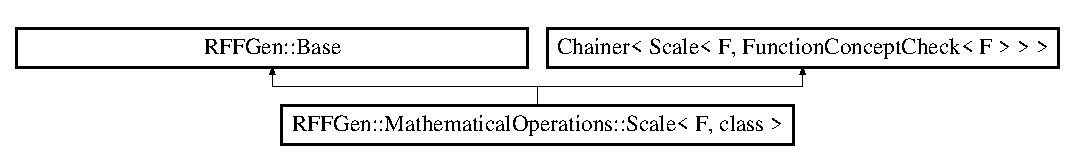
\includegraphics[height=1.717791cm]{structRFFGen_1_1MathematicalOperations_1_1Scale}
\end{center}
\end{figure}
\subsection*{Public Member Functions}
\begin{DoxyCompactItemize}
\item 
\hypertarget{structRFFGen_1_1MathematicalOperations_1_1Scale_af8fabe28c4a3bfbb5468ceccc1efbec2}{\hyperlink{structRFFGen_1_1MathematicalOperations_1_1Scale_af8fabe28c4a3bfbb5468ceccc1efbec2}{Scale} ()=default}\label{structRFFGen_1_1MathematicalOperations_1_1Scale_af8fabe28c4a3bfbb5468ceccc1efbec2}

\begin{DoxyCompactList}\small\item\em Default constructor. May leave member variables uninitialized! Call update before using evaluation. \end{DoxyCompactList}\item 
{\footnotesize template$<$class Init\-F $>$ }\\\hyperlink{structRFFGen_1_1MathematicalOperations_1_1Scale_a93e5aa65f4fa7f496691e259dbc06c98}{Scale} (double a\-\_\-, const Init\-F \&f\-\_\-)
\begin{DoxyCompactList}\small\item\em Constructor passing arguments to function constructor. \end{DoxyCompactList}\item 
\hypertarget{structRFFGen_1_1MathematicalOperations_1_1Scale_aca94d08d0113284e8d70f6bca9638952}{{\footnotesize template$<$class Arg $>$ }\\void \hyperlink{structRFFGen_1_1MathematicalOperations_1_1Scale_aca94d08d0113284e8d70f6bca9638952}{update} (Arg const \&arg)}\label{structRFFGen_1_1MathematicalOperations_1_1Scale_aca94d08d0113284e8d70f6bca9638952}

\begin{DoxyCompactList}\small\item\em Reset point of evaluation. \end{DoxyCompactList}\item 
\hypertarget{structRFFGen_1_1MathematicalOperations_1_1Scale_ad90664cd65d9f0f4911a47836d21a31b}{{\footnotesize template$<$int index, class Arg $>$ }\\void \hyperlink{structRFFGen_1_1MathematicalOperations_1_1Scale_ad90664cd65d9f0f4911a47836d21a31b}{update\-Variable} (const Arg \&x)}\label{structRFFGen_1_1MathematicalOperations_1_1Scale_ad90664cd65d9f0f4911a47836d21a31b}

\begin{DoxyCompactList}\small\item\em Propagate call to \hyperlink{structRFFGen_1_1MathematicalOperations_1_1Scale_ad90664cd65d9f0f4911a47836d21a31b}{update\-Variable()} to f. \end{DoxyCompactList}\item 
\hypertarget{structRFFGen_1_1MathematicalOperations_1_1Scale_a9e89fc6fa01ddd2a9b0e056f5d010aba}{const auto \& \hyperlink{structRFFGen_1_1MathematicalOperations_1_1Scale_a9e89fc6fa01ddd2a9b0e056f5d010aba}{d0} () const noexcept}\label{structRFFGen_1_1MathematicalOperations_1_1Scale_a9e89fc6fa01ddd2a9b0e056f5d010aba}

\begin{DoxyCompactList}\small\item\em Function value. \end{DoxyCompactList}\item 
{\footnotesize template$<$int idx, class Arg , class Indexed\-Arg  = Indexed\-Type$<$\-Arg,idx$>$, class  = std\-::enable\-\_\-if\-\_\-t$<$ D1$<$\-F,\-Indexed\-Arg$>$\-::present$>$$>$ }\\auto \hyperlink{structRFFGen_1_1MathematicalOperations_1_1Scale_a772e3b13af33837d70f5ceadc08fd97a}{d1} (Arg const \&dx) const 
\begin{DoxyCompactList}\small\item\em First directional derivative. \end{DoxyCompactList}\item 
{\footnotesize template$<$int idx, int idy, class Arg\-X , class Arg\-Y , class Indexed\-Arg\-X  = Indexed\-Type$<$\-Arg\-X,idx$>$, class Indexed\-Arg\-Y  = Indexed\-Type$<$\-Arg\-Y,idy$>$, class  = std\-::enable\-\_\-if\-\_\-t$<$ D2$<$\-F,\-Indexed\-Arg\-X,\-Indexed\-Arg\-Y$>$\-::present$>$$>$ }\\auto \hyperlink{structRFFGen_1_1MathematicalOperations_1_1Scale_a49b3374055d675325902fc8ba9a15b64}{d2} (Arg\-X const \&dx, Arg\-Y const \&dy) const 
\begin{DoxyCompactList}\small\item\em Second directional derivative. \end{DoxyCompactList}\item 
{\footnotesize template$<$int idx, int idy, int idz, class Arg\-X , class Arg\-Y , class Arg\-Z , class Indexed\-Arg\-X  = Indexed\-Type$<$\-Arg\-X,idx$>$, class Indexed\-Arg\-Y  = Indexed\-Type$<$\-Arg\-Y,idy$>$, class Indexed\-Arg\-Z  = Indexed\-Type$<$\-Arg\-Z,idz$>$, class  = std\-::enable\-\_\-if\-\_\-t$<$ D3$<$\-F,\-Indexed\-Arg\-X,\-Indexed\-Arg\-Y,\-Indexed\-Arg\-Z$>$\-::present $>$$>$ }\\auto \hyperlink{structRFFGen_1_1MathematicalOperations_1_1Scale_a087f60036322f4884121528871a15059}{d3} (Arg\-X const \&dx, Arg\-Y const \&dy, Arg\-Z const \&dz) const 
\begin{DoxyCompactList}\small\item\em Third directional derivative. \end{DoxyCompactList}\end{DoxyCompactItemize}


\subsection{Detailed Description}
\subsubsection*{template$<$class F, class = Function\-Concept\-Check$<$\-F$>$$>$struct R\-F\-F\-Gen\-::\-Mathematical\-Operations\-::\-Scale$<$ F, class $>$}

Scaling $ af $ of some function $ f $ with a double $ a $ (F must satisfy the requirements of \hyperlink{structRFFGen_1_1Concepts_1_1FunctionConcept}{Concepts\-::\-Function\-Concept}). 

\subsection{Constructor \& Destructor Documentation}
\hypertarget{structRFFGen_1_1MathematicalOperations_1_1Scale_a93e5aa65f4fa7f496691e259dbc06c98}{\index{R\-F\-F\-Gen\-::\-Mathematical\-Operations\-::\-Scale@{R\-F\-F\-Gen\-::\-Mathematical\-Operations\-::\-Scale}!Scale@{Scale}}
\index{Scale@{Scale}!RFFGen::MathematicalOperations::Scale@{R\-F\-F\-Gen\-::\-Mathematical\-Operations\-::\-Scale}}
\subsubsection[{Scale}]{\setlength{\rightskip}{0pt plus 5cm}template$<$class F , class  = Function\-Concept\-Check$<$\-F$>$$>$ template$<$class Init\-F $>$ {\bf R\-F\-F\-Gen\-::\-Mathematical\-Operations\-::\-Scale}$<$ F, class $>$\-::{\bf Scale} (
\begin{DoxyParamCaption}
\item[{double}]{a\-\_\-, }
\item[{const Init\-F \&}]{f\-\_\-}
\end{DoxyParamCaption}
)\hspace{0.3cm}{\ttfamily [inline]}}}\label{structRFFGen_1_1MathematicalOperations_1_1Scale_a93e5aa65f4fa7f496691e259dbc06c98}


Constructor passing arguments to function constructor. 


\begin{DoxyParams}{Parameters}
{\em a\-\_\-} & scaling \\
\hline
{\em f\-\_\-} & input for constructor of outer function \\
\hline
\end{DoxyParams}


\subsection{Member Function Documentation}
\hypertarget{structRFFGen_1_1MathematicalOperations_1_1Scale_a772e3b13af33837d70f5ceadc08fd97a}{\index{R\-F\-F\-Gen\-::\-Mathematical\-Operations\-::\-Scale@{R\-F\-F\-Gen\-::\-Mathematical\-Operations\-::\-Scale}!d1@{d1}}
\index{d1@{d1}!RFFGen::MathematicalOperations::Scale@{R\-F\-F\-Gen\-::\-Mathematical\-Operations\-::\-Scale}}
\subsubsection[{d1}]{\setlength{\rightskip}{0pt plus 5cm}template$<$class F , class  = Function\-Concept\-Check$<$\-F$>$$>$ template$<$int idx, class Arg , class Indexed\-Arg  = Indexed\-Type$<$\-Arg,idx$>$, class  = std\-::enable\-\_\-if\-\_\-t$<$ D1$<$\-F,\-Indexed\-Arg$>$\-::present$>$$>$ auto {\bf R\-F\-F\-Gen\-::\-Mathematical\-Operations\-::\-Scale}$<$ F, class $>$\-::d1 (
\begin{DoxyParamCaption}
\item[{Arg const \&}]{dx}
\end{DoxyParamCaption}
) const\hspace{0.3cm}{\ttfamily [inline]}}}\label{structRFFGen_1_1MathematicalOperations_1_1Scale_a772e3b13af33837d70f5ceadc08fd97a}


First directional derivative. 


\begin{DoxyParams}{Parameters}
{\em dx} & direction for which the derivative is computed \\
\hline
\end{DoxyParams}
\hypertarget{structRFFGen_1_1MathematicalOperations_1_1Scale_a49b3374055d675325902fc8ba9a15b64}{\index{R\-F\-F\-Gen\-::\-Mathematical\-Operations\-::\-Scale@{R\-F\-F\-Gen\-::\-Mathematical\-Operations\-::\-Scale}!d2@{d2}}
\index{d2@{d2}!RFFGen::MathematicalOperations::Scale@{R\-F\-F\-Gen\-::\-Mathematical\-Operations\-::\-Scale}}
\subsubsection[{d2}]{\setlength{\rightskip}{0pt plus 5cm}template$<$class F , class  = Function\-Concept\-Check$<$\-F$>$$>$ template$<$int idx, int idy, class Arg\-X , class Arg\-Y , class Indexed\-Arg\-X  = Indexed\-Type$<$\-Arg\-X,idx$>$, class Indexed\-Arg\-Y  = Indexed\-Type$<$\-Arg\-Y,idy$>$, class  = std\-::enable\-\_\-if\-\_\-t$<$ D2$<$\-F,\-Indexed\-Arg\-X,\-Indexed\-Arg\-Y$>$\-::present$>$$>$ auto {\bf R\-F\-F\-Gen\-::\-Mathematical\-Operations\-::\-Scale}$<$ F, class $>$\-::d2 (
\begin{DoxyParamCaption}
\item[{Arg\-X const \&}]{dx, }
\item[{Arg\-Y const \&}]{dy}
\end{DoxyParamCaption}
) const\hspace{0.3cm}{\ttfamily [inline]}}}\label{structRFFGen_1_1MathematicalOperations_1_1Scale_a49b3374055d675325902fc8ba9a15b64}


Second directional derivative. 


\begin{DoxyParams}{Parameters}
{\em dx} & direction for which the derivative is computed \\
\hline
{\em dy} & direction for which the derivative is computed \\
\hline
\end{DoxyParams}
\hypertarget{structRFFGen_1_1MathematicalOperations_1_1Scale_a087f60036322f4884121528871a15059}{\index{R\-F\-F\-Gen\-::\-Mathematical\-Operations\-::\-Scale@{R\-F\-F\-Gen\-::\-Mathematical\-Operations\-::\-Scale}!d3@{d3}}
\index{d3@{d3}!RFFGen::MathematicalOperations::Scale@{R\-F\-F\-Gen\-::\-Mathematical\-Operations\-::\-Scale}}
\subsubsection[{d3}]{\setlength{\rightskip}{0pt plus 5cm}template$<$class F , class  = Function\-Concept\-Check$<$\-F$>$$>$ template$<$int idx, int idy, int idz, class Arg\-X , class Arg\-Y , class Arg\-Z , class Indexed\-Arg\-X  = Indexed\-Type$<$\-Arg\-X,idx$>$, class Indexed\-Arg\-Y  = Indexed\-Type$<$\-Arg\-Y,idy$>$, class Indexed\-Arg\-Z  = Indexed\-Type$<$\-Arg\-Z,idz$>$, class  = std\-::enable\-\_\-if\-\_\-t$<$ D3$<$\-F,\-Indexed\-Arg\-X,\-Indexed\-Arg\-Y,\-Indexed\-Arg\-Z$>$\-::present $>$$>$ auto {\bf R\-F\-F\-Gen\-::\-Mathematical\-Operations\-::\-Scale}$<$ F, class $>$\-::d3 (
\begin{DoxyParamCaption}
\item[{Arg\-X const \&}]{dx, }
\item[{Arg\-Y const \&}]{dy, }
\item[{Arg\-Z const \&}]{dz}
\end{DoxyParamCaption}
) const\hspace{0.3cm}{\ttfamily [inline]}}}\label{structRFFGen_1_1MathematicalOperations_1_1Scale_a087f60036322f4884121528871a15059}


Third directional derivative. 


\begin{DoxyParams}{Parameters}
{\em dx} & direction for which the derivative is computed \\
\hline
{\em dy} & direction for which the derivative is computed \\
\hline
{\em dz} & direction for which the derivative is computed \\
\hline
\end{DoxyParams}


The documentation for this struct was generated from the following file\-:\begin{DoxyCompactItemize}
\item 
R\-F\-F\-Gen/\-Mathematical\-Operations/scale.\-hh\end{DoxyCompactItemize}

\hypertarget{structRFFGen_1_1LinearAlgebra_1_1SecondModifiedMixedInvariant}{\section{R\-F\-F\-Gen\-:\-:Linear\-Algebra\-:\-:Second\-Modified\-Mixed\-Invariant$<$ Matrix, class $>$ Struct Template Reference}
\label{structRFFGen_1_1LinearAlgebra_1_1SecondModifiedMixedInvariant}\index{R\-F\-F\-Gen\-::\-Linear\-Algebra\-::\-Second\-Modified\-Mixed\-Invariant$<$ Matrix, class $>$@{R\-F\-F\-Gen\-::\-Linear\-Algebra\-::\-Second\-Modified\-Mixed\-Invariant$<$ Matrix, class $>$}}
}


Second modified mixed invariant $\bar\iota_5=\iota_5\iota_3^{-2/3}$.  




{\ttfamily \#include $<$modified\-Mixed\-Invariants.\-hh$>$}

Inheritance diagram for R\-F\-F\-Gen\-:\-:Linear\-Algebra\-:\-:Second\-Modified\-Mixed\-Invariant$<$ Matrix, class $>$\-:\begin{figure}[H]
\begin{center}
\leavevmode
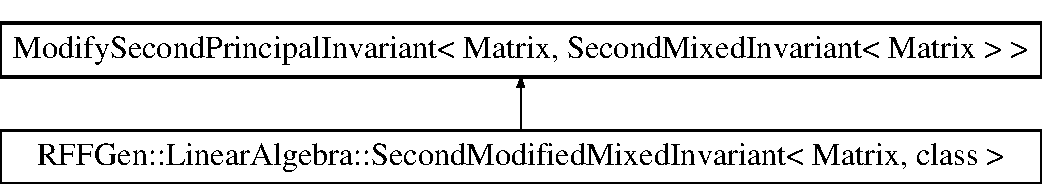
\includegraphics[height=2.000000cm]{structRFFGen_1_1LinearAlgebra_1_1SecondModifiedMixedInvariant}
\end{center}
\end{figure}
\subsection*{Public Member Functions}
\begin{DoxyCompactItemize}
\item 
\hypertarget{structRFFGen_1_1LinearAlgebra_1_1SecondModifiedMixedInvariant_a616648819b50566888bbd3ecce020db0}{\hyperlink{structRFFGen_1_1LinearAlgebra_1_1SecondModifiedMixedInvariant_a616648819b50566888bbd3ecce020db0}{Second\-Modified\-Mixed\-Invariant} ()=default}\label{structRFFGen_1_1LinearAlgebra_1_1SecondModifiedMixedInvariant_a616648819b50566888bbd3ecce020db0}

\begin{DoxyCompactList}\small\item\em Default constructor. \end{DoxyCompactList}\item 
\hyperlink{structRFFGen_1_1LinearAlgebra_1_1SecondModifiedMixedInvariant_aa23bb41771ecbde5618a83dfb2555ecd}{Second\-Modified\-Mixed\-Invariant} (const Matrix \&A, const \hyperlink{structRFFGen_1_1Constant}{Constant}$<$ Matrix $>$ \&M)
\begin{DoxyCompactList}\small\item\em Constructor. \end{DoxyCompactList}\item 
\hyperlink{structRFFGen_1_1LinearAlgebra_1_1SecondModifiedMixedInvariant_aabe601389efe990b50642f63508742c1}{Second\-Modified\-Mixed\-Invariant} (const std\-::tuple$<$ Matrix, \hyperlink{structRFFGen_1_1Constant}{Constant}$<$ Matrix $>$ $>$ \&t)
\begin{DoxyCompactList}\small\item\em Constructor from std\-::tuple. \end{DoxyCompactList}\end{DoxyCompactItemize}


\subsection{Detailed Description}
\subsubsection*{template$<$class Matrix, class = Concepts\-::\-Symmetric\-Matrix\-Concept\-Check$<$\-Matrix$>$$>$struct R\-F\-F\-Gen\-::\-Linear\-Algebra\-::\-Second\-Modified\-Mixed\-Invariant$<$ Matrix, class $>$}

Second modified mixed invariant $\bar\iota_5=\iota_5\iota_3^{-2/3}$. 

\subsection{Constructor \& Destructor Documentation}
\hypertarget{structRFFGen_1_1LinearAlgebra_1_1SecondModifiedMixedInvariant_aa23bb41771ecbde5618a83dfb2555ecd}{\index{R\-F\-F\-Gen\-::\-Linear\-Algebra\-::\-Second\-Modified\-Mixed\-Invariant@{R\-F\-F\-Gen\-::\-Linear\-Algebra\-::\-Second\-Modified\-Mixed\-Invariant}!Second\-Modified\-Mixed\-Invariant@{Second\-Modified\-Mixed\-Invariant}}
\index{Second\-Modified\-Mixed\-Invariant@{Second\-Modified\-Mixed\-Invariant}!RFFGen::LinearAlgebra::SecondModifiedMixedInvariant@{R\-F\-F\-Gen\-::\-Linear\-Algebra\-::\-Second\-Modified\-Mixed\-Invariant}}
\subsubsection[{Second\-Modified\-Mixed\-Invariant}]{\setlength{\rightskip}{0pt plus 5cm}template$<$class Matrix , class  = Concepts\-::\-Symmetric\-Matrix\-Concept\-Check$<$\-Matrix$>$$>$ {\bf R\-F\-F\-Gen\-::\-Linear\-Algebra\-::\-Second\-Modified\-Mixed\-Invariant}$<$ Matrix, class $>$\-::{\bf Second\-Modified\-Mixed\-Invariant} (
\begin{DoxyParamCaption}
\item[{const Matrix \&}]{A, }
\item[{const {\bf Constant}$<$ Matrix $>$ \&}]{M}
\end{DoxyParamCaption}
)\hspace{0.3cm}{\ttfamily [inline]}}}\label{structRFFGen_1_1LinearAlgebra_1_1SecondModifiedMixedInvariant_aa23bb41771ecbde5618a83dfb2555ecd}


Constructor. 


\begin{DoxyParams}{Parameters}
{\em A} & matrix to compute second modified mixed invariant from. \\
\hline
{\em M} & structural tensor incorporating anisotropic information. \\
\hline
\end{DoxyParams}
\hypertarget{structRFFGen_1_1LinearAlgebra_1_1SecondModifiedMixedInvariant_aabe601389efe990b50642f63508742c1}{\index{R\-F\-F\-Gen\-::\-Linear\-Algebra\-::\-Second\-Modified\-Mixed\-Invariant@{R\-F\-F\-Gen\-::\-Linear\-Algebra\-::\-Second\-Modified\-Mixed\-Invariant}!Second\-Modified\-Mixed\-Invariant@{Second\-Modified\-Mixed\-Invariant}}
\index{Second\-Modified\-Mixed\-Invariant@{Second\-Modified\-Mixed\-Invariant}!RFFGen::LinearAlgebra::SecondModifiedMixedInvariant@{R\-F\-F\-Gen\-::\-Linear\-Algebra\-::\-Second\-Modified\-Mixed\-Invariant}}
\subsubsection[{Second\-Modified\-Mixed\-Invariant}]{\setlength{\rightskip}{0pt plus 5cm}template$<$class Matrix , class  = Concepts\-::\-Symmetric\-Matrix\-Concept\-Check$<$\-Matrix$>$$>$ {\bf R\-F\-F\-Gen\-::\-Linear\-Algebra\-::\-Second\-Modified\-Mixed\-Invariant}$<$ Matrix, class $>$\-::{\bf Second\-Modified\-Mixed\-Invariant} (
\begin{DoxyParamCaption}
\item[{const std\-::tuple$<$ Matrix, {\bf Constant}$<$ Matrix $>$ $>$ \&}]{t}
\end{DoxyParamCaption}
)\hspace{0.3cm}{\ttfamily [inline]}}}\label{structRFFGen_1_1LinearAlgebra_1_1SecondModifiedMixedInvariant_aabe601389efe990b50642f63508742c1}


Constructor from std\-::tuple. 


\begin{DoxyParams}{Parameters}
{\em t} & st\-::get$<$0$>$(t)\-: matrix to compute second modified invariant form, std\-::get$<$1$>$(t)\-: structural tensor \\
\hline
\end{DoxyParams}


The documentation for this struct was generated from the following file\-:\begin{DoxyCompactItemize}
\item 
R\-F\-F\-Gen/\-Linear\-Algebra/modified\-Mixed\-Invariants.\-hh\end{DoxyCompactItemize}

\hypertarget{structRFFGen_1_1LinearAlgebra_1_1SecondModifiedPrincipalInvariant}{\section{R\-F\-F\-Gen\-:\-:Linear\-Algebra\-:\-:Second\-Modified\-Principal\-Invariant$<$ Matrix, class $>$ Struct Template Reference}
\label{structRFFGen_1_1LinearAlgebra_1_1SecondModifiedPrincipalInvariant}\index{R\-F\-F\-Gen\-::\-Linear\-Algebra\-::\-Second\-Modified\-Principal\-Invariant$<$ Matrix, class $>$@{R\-F\-F\-Gen\-::\-Linear\-Algebra\-::\-Second\-Modified\-Principal\-Invariant$<$ Matrix, class $>$}}
}


Isochoric (volume-\/preserving), second modified principal invariant $ \bar\iota_2(A)=\iota_2\iota_3^{-1/3} $, where $\iota_2$ is the second and $\iota_3$ is the third principal invariant.  




{\ttfamily \#include $<$modified\-Principal\-Invariants.\-hh$>$}

Inheritance diagram for R\-F\-F\-Gen\-:\-:Linear\-Algebra\-:\-:Second\-Modified\-Principal\-Invariant$<$ Matrix, class $>$\-:\begin{figure}[H]
\begin{center}
\leavevmode
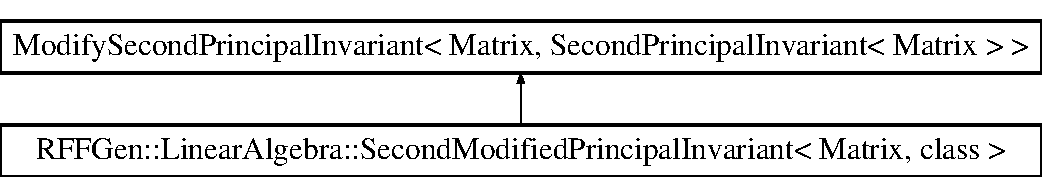
\includegraphics[height=2.000000cm]{structRFFGen_1_1LinearAlgebra_1_1SecondModifiedPrincipalInvariant}
\end{center}
\end{figure}
\subsection*{Public Member Functions}
\begin{DoxyCompactItemize}
\item 
\hypertarget{structRFFGen_1_1LinearAlgebra_1_1SecondModifiedPrincipalInvariant_ae7e278ae20ef756aeb2281a0cd6eed39}{\hyperlink{structRFFGen_1_1LinearAlgebra_1_1SecondModifiedPrincipalInvariant_ae7e278ae20ef756aeb2281a0cd6eed39}{Second\-Modified\-Principal\-Invariant} ()=default}\label{structRFFGen_1_1LinearAlgebra_1_1SecondModifiedPrincipalInvariant_ae7e278ae20ef756aeb2281a0cd6eed39}

\begin{DoxyCompactList}\small\item\em Default constructor. \end{DoxyCompactList}\item 
\hyperlink{structRFFGen_1_1LinearAlgebra_1_1SecondModifiedPrincipalInvariant_a4c7ced997d5086bce88bbba02ad7aeb9}{Second\-Modified\-Principal\-Invariant} (const Matrix \&A)
\begin{DoxyCompactList}\small\item\em Constructor. \end{DoxyCompactList}\end{DoxyCompactItemize}


\subsection{Detailed Description}
\subsubsection*{template$<$class Matrix, class = Concepts\-::\-Symmetric\-Matrix\-Concept\-Check$<$\-Matrix$>$$>$struct R\-F\-F\-Gen\-::\-Linear\-Algebra\-::\-Second\-Modified\-Principal\-Invariant$<$ Matrix, class $>$}

Isochoric (volume-\/preserving), second modified principal invariant $ \bar\iota_2(A)=\iota_2\iota_3^{-1/3} $, where $\iota_2$ is the second and $\iota_3$ is the third principal invariant. 

\subsection{Constructor \& Destructor Documentation}
\hypertarget{structRFFGen_1_1LinearAlgebra_1_1SecondModifiedPrincipalInvariant_a4c7ced997d5086bce88bbba02ad7aeb9}{\index{R\-F\-F\-Gen\-::\-Linear\-Algebra\-::\-Second\-Modified\-Principal\-Invariant@{R\-F\-F\-Gen\-::\-Linear\-Algebra\-::\-Second\-Modified\-Principal\-Invariant}!Second\-Modified\-Principal\-Invariant@{Second\-Modified\-Principal\-Invariant}}
\index{Second\-Modified\-Principal\-Invariant@{Second\-Modified\-Principal\-Invariant}!RFFGen::LinearAlgebra::SecondModifiedPrincipalInvariant@{R\-F\-F\-Gen\-::\-Linear\-Algebra\-::\-Second\-Modified\-Principal\-Invariant}}
\subsubsection[{Second\-Modified\-Principal\-Invariant}]{\setlength{\rightskip}{0pt plus 5cm}template$<$class Matrix , class  = Concepts\-::\-Symmetric\-Matrix\-Concept\-Check$<$\-Matrix$>$$>$ {\bf R\-F\-F\-Gen\-::\-Linear\-Algebra\-::\-Second\-Modified\-Principal\-Invariant}$<$ Matrix, class $>$\-::{\bf Second\-Modified\-Principal\-Invariant} (
\begin{DoxyParamCaption}
\item[{const Matrix \&}]{A}
\end{DoxyParamCaption}
)\hspace{0.3cm}{\ttfamily [inline]}}}\label{structRFFGen_1_1LinearAlgebra_1_1SecondModifiedPrincipalInvariant_a4c7ced997d5086bce88bbba02ad7aeb9}


Constructor. 


\begin{DoxyParams}{Parameters}
{\em A} & matrix to compute second modified principal invariant from. \\
\hline
\end{DoxyParams}


The documentation for this struct was generated from the following file\-:\begin{DoxyCompactItemize}
\item 
R\-F\-F\-Gen/\-Linear\-Algebra/modified\-Principal\-Invariants.\-hh\end{DoxyCompactItemize}

\hypertarget{classRFFGen_1_1LinearAlgebra_1_1SecondPrincipalInvariant}{\section{R\-F\-F\-Gen\-:\-:Linear\-Algebra\-:\-:Second\-Principal\-Invariant$<$ Matrix, class $>$ Class Template Reference}
\label{classRFFGen_1_1LinearAlgebra_1_1SecondPrincipalInvariant}\index{R\-F\-F\-Gen\-::\-Linear\-Algebra\-::\-Second\-Principal\-Invariant$<$ Matrix, class $>$@{R\-F\-F\-Gen\-::\-Linear\-Algebra\-::\-Second\-Principal\-Invariant$<$ Matrix, class $>$}}
}


Second principal invariant $ \iota_2(A)=\mathrm{tr}(\mathrm{cof}(A)) $ for $A\in\mathbb{R}^{n,n}$.  




{\ttfamily \#include $<$principal\-Invariants.\-hh$>$}

Inheritance diagram for R\-F\-F\-Gen\-:\-:Linear\-Algebra\-:\-:Second\-Principal\-Invariant$<$ Matrix, class $>$\-:\begin{figure}[H]
\begin{center}
\leavevmode
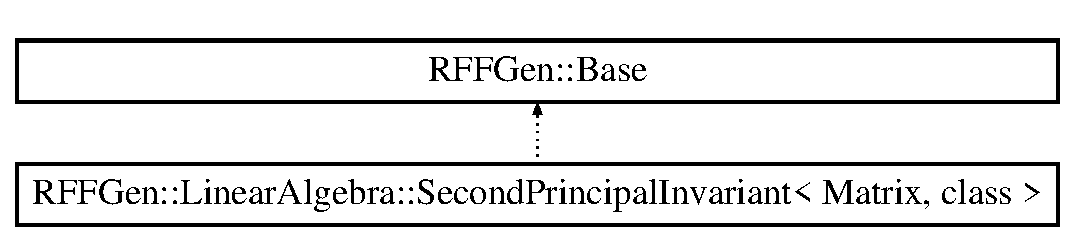
\includegraphics[height=2.000000cm]{classRFFGen_1_1LinearAlgebra_1_1SecondPrincipalInvariant}
\end{center}
\end{figure}
\subsection*{Public Member Functions}
\begin{DoxyCompactItemize}
\item 
\hypertarget{classRFFGen_1_1LinearAlgebra_1_1SecondPrincipalInvariant_a61eb0b2c86c253d6a5cbb23c3260cf5a}{\hyperlink{classRFFGen_1_1LinearAlgebra_1_1SecondPrincipalInvariant_a61eb0b2c86c253d6a5cbb23c3260cf5a}{Second\-Principal\-Invariant} ()=default}\label{classRFFGen_1_1LinearAlgebra_1_1SecondPrincipalInvariant_a61eb0b2c86c253d6a5cbb23c3260cf5a}

\begin{DoxyCompactList}\small\item\em Default constructor. \end{DoxyCompactList}\item 
\hyperlink{classRFFGen_1_1LinearAlgebra_1_1SecondPrincipalInvariant_ad9aa80cca5fbd2247ecb75e0bfd7775e}{Second\-Principal\-Invariant} (const Matrix \&A)
\begin{DoxyCompactList}\small\item\em Constructor. \end{DoxyCompactList}\item 
\hypertarget{classRFFGen_1_1LinearAlgebra_1_1SecondPrincipalInvariant_a373b805f57413a22f15c472e1967e244}{void \hyperlink{classRFFGen_1_1LinearAlgebra_1_1SecondPrincipalInvariant_a373b805f57413a22f15c472e1967e244}{update} (const Matrix \&A)}\label{classRFFGen_1_1LinearAlgebra_1_1SecondPrincipalInvariant_a373b805f57413a22f15c472e1967e244}

\begin{DoxyCompactList}\small\item\em Reset matrix to compute second principal invariant from. \end{DoxyCompactList}\item 
\hypertarget{classRFFGen_1_1LinearAlgebra_1_1SecondPrincipalInvariant_a73cf245582d0f3bd0a5702b175a78537}{auto \hyperlink{classRFFGen_1_1LinearAlgebra_1_1SecondPrincipalInvariant_a73cf245582d0f3bd0a5702b175a78537}{d0} () const }\label{classRFFGen_1_1LinearAlgebra_1_1SecondPrincipalInvariant_a73cf245582d0f3bd0a5702b175a78537}

\begin{DoxyCompactList}\small\item\em Value of the second principal invariant. \end{DoxyCompactList}\item 
{\footnotesize template$<$int , int $>$ }\\auto \hyperlink{classRFFGen_1_1LinearAlgebra_1_1SecondPrincipalInvariant_a411b252232f2d2a4332f5f22fab5e805}{d1} (const Matrix \&d\-A1) const 
\begin{DoxyCompactList}\small\item\em First directional derivative. \end{DoxyCompactList}\item 
{\footnotesize template$<$int , int $>$ }\\auto \hyperlink{classRFFGen_1_1LinearAlgebra_1_1SecondPrincipalInvariant_a8814f8f93d1f6fa547ff32e95669aa93}{d2} (const Matrix \&d\-A1, const Matrix \&d\-A2) const 
\begin{DoxyCompactList}\small\item\em Second directional derivative. \end{DoxyCompactList}\end{DoxyCompactItemize}


\subsection{Detailed Description}
\subsubsection*{template$<$class Matrix, class = Concepts\-::\-Symmetric\-Matrix\-Concept\-Check$<$\-Matrix$>$$>$class R\-F\-F\-Gen\-::\-Linear\-Algebra\-::\-Second\-Principal\-Invariant$<$ Matrix, class $>$}

Second principal invariant $ \iota_2(A)=\mathrm{tr}(\mathrm{cof}(A)) $ for $A\in\mathbb{R}^{n,n}$. 

\subsection{Constructor \& Destructor Documentation}
\hypertarget{classRFFGen_1_1LinearAlgebra_1_1SecondPrincipalInvariant_ad9aa80cca5fbd2247ecb75e0bfd7775e}{\index{R\-F\-F\-Gen\-::\-Linear\-Algebra\-::\-Second\-Principal\-Invariant@{R\-F\-F\-Gen\-::\-Linear\-Algebra\-::\-Second\-Principal\-Invariant}!Second\-Principal\-Invariant@{Second\-Principal\-Invariant}}
\index{Second\-Principal\-Invariant@{Second\-Principal\-Invariant}!RFFGen::LinearAlgebra::SecondPrincipalInvariant@{R\-F\-F\-Gen\-::\-Linear\-Algebra\-::\-Second\-Principal\-Invariant}}
\subsubsection[{Second\-Principal\-Invariant}]{\setlength{\rightskip}{0pt plus 5cm}template$<$class Matrix , class  = Concepts\-::\-Symmetric\-Matrix\-Concept\-Check$<$\-Matrix$>$$>$ {\bf R\-F\-F\-Gen\-::\-Linear\-Algebra\-::\-Second\-Principal\-Invariant}$<$ Matrix, class $>$\-::{\bf Second\-Principal\-Invariant} (
\begin{DoxyParamCaption}
\item[{const Matrix \&}]{A}
\end{DoxyParamCaption}
)\hspace{0.3cm}{\ttfamily [inline]}}}\label{classRFFGen_1_1LinearAlgebra_1_1SecondPrincipalInvariant_ad9aa80cca5fbd2247ecb75e0bfd7775e}


Constructor. 


\begin{DoxyParams}{Parameters}
{\em A} & matrix to compute second principal invariant from \\
\hline
\end{DoxyParams}


\subsection{Member Function Documentation}
\hypertarget{classRFFGen_1_1LinearAlgebra_1_1SecondPrincipalInvariant_a411b252232f2d2a4332f5f22fab5e805}{\index{R\-F\-F\-Gen\-::\-Linear\-Algebra\-::\-Second\-Principal\-Invariant@{R\-F\-F\-Gen\-::\-Linear\-Algebra\-::\-Second\-Principal\-Invariant}!d1@{d1}}
\index{d1@{d1}!RFFGen::LinearAlgebra::SecondPrincipalInvariant@{R\-F\-F\-Gen\-::\-Linear\-Algebra\-::\-Second\-Principal\-Invariant}}
\subsubsection[{d1}]{\setlength{\rightskip}{0pt plus 5cm}template$<$class Matrix , class  = Concepts\-::\-Symmetric\-Matrix\-Concept\-Check$<$\-Matrix$>$$>$ template$<$int , int $>$ auto {\bf R\-F\-F\-Gen\-::\-Linear\-Algebra\-::\-Second\-Principal\-Invariant}$<$ Matrix, class $>$\-::d1 (
\begin{DoxyParamCaption}
\item[{const Matrix \&}]{d\-A1}
\end{DoxyParamCaption}
) const\hspace{0.3cm}{\ttfamily [inline]}}}\label{classRFFGen_1_1LinearAlgebra_1_1SecondPrincipalInvariant_a411b252232f2d2a4332f5f22fab5e805}


First directional derivative. 


\begin{DoxyParams}{Parameters}
{\em d\-A1} & direction for which the derivative is computed \\
\hline
\end{DoxyParams}
\hypertarget{classRFFGen_1_1LinearAlgebra_1_1SecondPrincipalInvariant_a8814f8f93d1f6fa547ff32e95669aa93}{\index{R\-F\-F\-Gen\-::\-Linear\-Algebra\-::\-Second\-Principal\-Invariant@{R\-F\-F\-Gen\-::\-Linear\-Algebra\-::\-Second\-Principal\-Invariant}!d2@{d2}}
\index{d2@{d2}!RFFGen::LinearAlgebra::SecondPrincipalInvariant@{R\-F\-F\-Gen\-::\-Linear\-Algebra\-::\-Second\-Principal\-Invariant}}
\subsubsection[{d2}]{\setlength{\rightskip}{0pt plus 5cm}template$<$class Matrix , class  = Concepts\-::\-Symmetric\-Matrix\-Concept\-Check$<$\-Matrix$>$$>$ template$<$int , int $>$ auto {\bf R\-F\-F\-Gen\-::\-Linear\-Algebra\-::\-Second\-Principal\-Invariant}$<$ Matrix, class $>$\-::d2 (
\begin{DoxyParamCaption}
\item[{const Matrix \&}]{d\-A1, }
\item[{const Matrix \&}]{d\-A2}
\end{DoxyParamCaption}
) const\hspace{0.3cm}{\ttfamily [inline]}}}\label{classRFFGen_1_1LinearAlgebra_1_1SecondPrincipalInvariant_a8814f8f93d1f6fa547ff32e95669aa93}


Second directional derivative. 


\begin{DoxyParams}{Parameters}
{\em d\-A1} & direction for which the derivative is computed \\
\hline
{\em d\-A2} & direction for which the derivative is computed \\
\hline
\end{DoxyParams}


The documentation for this class was generated from the following file\-:\begin{DoxyCompactItemize}
\item 
R\-F\-F\-Gen/\-Linear\-Algebra/principal\-Invariants.\-hh\end{DoxyCompactItemize}

\hypertarget{classRFFGen_1_1LinearAlgebra_1_1ShiftedInvariant}{\section{R\-F\-F\-Gen\-:\-:Linear\-Algebra\-:\-:Shifted\-Invariant$<$ Invariant, offset $>$ Class Template Reference}
\label{classRFFGen_1_1LinearAlgebra_1_1ShiftedInvariant}\index{R\-F\-F\-Gen\-::\-Linear\-Algebra\-::\-Shifted\-Invariant$<$ Invariant, offset $>$@{R\-F\-F\-Gen\-::\-Linear\-Algebra\-::\-Shifted\-Invariant$<$ Invariant, offset $>$}}
}


Possibly scaled, shifted invariant $scaling (invariant - offset)$, where $offset = dim$ for the first two (principal,modified) invariants and $offset = 1$ for the third (principal,modified) and mixed invariants.  




{\ttfamily \#include $<$shifted\-Invariant.\-hh$>$}

Inheritance diagram for R\-F\-F\-Gen\-:\-:Linear\-Algebra\-:\-:Shifted\-Invariant$<$ Invariant, offset $>$\-:\begin{figure}[H]
\begin{center}
\leavevmode
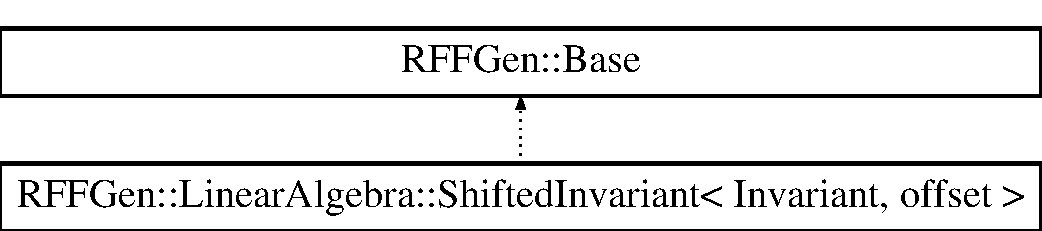
\includegraphics[height=2.000000cm]{classRFFGen_1_1LinearAlgebra_1_1ShiftedInvariant}
\end{center}
\end{figure}
\subsection*{Public Member Functions}
\begin{DoxyCompactItemize}
\item 
{\footnotesize template$<$class Matrix $>$ }\\\hyperlink{classRFFGen_1_1LinearAlgebra_1_1ShiftedInvariant_aebc264a312f0efff2ae7467d98eced75}{Shifted\-Invariant} (Matrix const \&A)
\item 
{\footnotesize template$<$class Matrix $>$ }\\\hyperlink{classRFFGen_1_1LinearAlgebra_1_1ShiftedInvariant_a52e0e4abd5099d9aa5b4ee1c73589adc}{Shifted\-Invariant} (const Matrix \&A, const \hyperlink{structRFFGen_1_1Constant}{Constant}$<$ Matrix $>$ \&M)
\item 
{\footnotesize template$<$class Matrix $>$ }\\\hyperlink{classRFFGen_1_1LinearAlgebra_1_1ShiftedInvariant_a2b15177fa88cd62ffec101d22ecea76e}{Shifted\-Invariant} (const Matrix \&A, const Matrix \&M)
\item 
\hypertarget{classRFFGen_1_1LinearAlgebra_1_1ShiftedInvariant_a89785734ed595d7e0c7e95562ef45400}{{\footnotesize template$<$class Matrix $>$ }\\void \hyperlink{classRFFGen_1_1LinearAlgebra_1_1ShiftedInvariant_a89785734ed595d7e0c7e95562ef45400}{update} (Matrix const \&A)}\label{classRFFGen_1_1LinearAlgebra_1_1ShiftedInvariant_a89785734ed595d7e0c7e95562ef45400}

\begin{DoxyCompactList}\small\item\em Reset matrix to compute shifted invariant from. \end{DoxyCompactList}\item 
\hypertarget{classRFFGen_1_1LinearAlgebra_1_1ShiftedInvariant_a4acc15ad6257a5871a5bf4da97efdbd8}{auto \hyperlink{classRFFGen_1_1LinearAlgebra_1_1ShiftedInvariant_a4acc15ad6257a5871a5bf4da97efdbd8}{d0} () const noexcept}\label{classRFFGen_1_1LinearAlgebra_1_1ShiftedInvariant_a4acc15ad6257a5871a5bf4da97efdbd8}

\begin{DoxyCompactList}\small\item\em Value of the shifted invariant. \end{DoxyCompactList}\item 
{\footnotesize template$<$int id, class Arg , class Indexed\-Arg  = Indexed\-Type$<$\-Arg,id$>$, class  = std\-::enable\-\_\-if\-\_\-t$<$\-Evaluate\-If\-Present$<$ D1$<$\-Invariant,\-Indexed\-Arg$>$ $>$\-::present$>$$>$ }\\auto \hyperlink{classRFFGen_1_1LinearAlgebra_1_1ShiftedInvariant_a4e05a73ae9cb190aee5bcb02332e7f36}{d1} (const Arg \&d\-A1) const 
\begin{DoxyCompactList}\small\item\em First directional derivative of the (scaled) shifted invariant. \end{DoxyCompactList}\item 
{\footnotesize template$<$int idx, int idy, class Arg\-X , class Arg\-Y , class Indexed\-Arg\-X  = Indexed\-Type$<$\-Arg\-X,idx$>$, class Indexed\-Arg\-Y  = Indexed\-Type$<$\-Arg\-Y,idx$>$, class  = std\-::enable\-\_\-if\-\_\-t$<$\-Evaluate\-If\-Present$<$ D2$<$\-Invariant,\-Indexed\-Arg\-X,\-Indexed\-Arg\-Y$>$ $>$\-::present$>$$>$ }\\auto \hyperlink{classRFFGen_1_1LinearAlgebra_1_1ShiftedInvariant_a3b1be101997bae58dcb305d63fe90505}{d2} (const Arg\-X \&d\-A1, const Arg\-Y \&d\-A2) const 
\begin{DoxyCompactList}\small\item\em Second directional derivative of the (scaled) shifted invariant. \end{DoxyCompactList}\item 
{\footnotesize template$<$int idx, int idy, int idz, class Arg\-X , class Arg\-Y , class Arg\-Z , class Indexed\-Arg\-X  = Indexed\-Type$<$\-Arg\-X,idx$>$, class Indexed\-Arg\-Y  = Indexed\-Type$<$\-Arg\-Y,idy$>$, class Indexed\-Arg\-Z  = Indexed\-Type$<$\-Arg\-Z,idz$>$, class  = std\-::enable\-\_\-if\-\_\-t$<$ Evaluate\-If\-Present$<$ D3$<$\-Invariant,\-Indexed\-Arg\-X,\-Indexed\-Arg\-Y,\-Indexed\-Arg\-Z$>$ $>$\-::present $>$$>$ }\\auto \hyperlink{classRFFGen_1_1LinearAlgebra_1_1ShiftedInvariant_a2467e5007ac8d84d11c1f68c15db03a4}{d3} (Arg\-X const \&d\-A1, Arg\-Y const \&d\-A2, Arg\-Z const \&d\-A3) const 
\begin{DoxyCompactList}\small\item\em Third directional derivative of the (scaled) shifted invariant. \end{DoxyCompactList}\end{DoxyCompactItemize}


\subsection{Detailed Description}
\subsubsection*{template$<$class Invariant, int offset$>$class R\-F\-F\-Gen\-::\-Linear\-Algebra\-::\-Shifted\-Invariant$<$ Invariant, offset $>$}

Possibly scaled, shifted invariant $scaling (invariant - offset)$, where $offset = dim$ for the first two (principal,modified) invariants and $offset = 1$ for the third (principal,modified) and mixed invariants. 

\subsection{Constructor \& Destructor Documentation}
\hypertarget{classRFFGen_1_1LinearAlgebra_1_1ShiftedInvariant_aebc264a312f0efff2ae7467d98eced75}{\index{R\-F\-F\-Gen\-::\-Linear\-Algebra\-::\-Shifted\-Invariant@{R\-F\-F\-Gen\-::\-Linear\-Algebra\-::\-Shifted\-Invariant}!Shifted\-Invariant@{Shifted\-Invariant}}
\index{Shifted\-Invariant@{Shifted\-Invariant}!RFFGen::LinearAlgebra::ShiftedInvariant@{R\-F\-F\-Gen\-::\-Linear\-Algebra\-::\-Shifted\-Invariant}}
\subsubsection[{Shifted\-Invariant}]{\setlength{\rightskip}{0pt plus 5cm}template$<$class Invariant , int offset$>$ template$<$class Matrix $>$ {\bf R\-F\-F\-Gen\-::\-Linear\-Algebra\-::\-Shifted\-Invariant}$<$ {\bf Invariant}, offset $>$\-::{\bf Shifted\-Invariant} (
\begin{DoxyParamCaption}
\item[{Matrix const \&}]{A}
\end{DoxyParamCaption}
)\hspace{0.3cm}{\ttfamily [inline]}}}\label{classRFFGen_1_1LinearAlgebra_1_1ShiftedInvariant_aebc264a312f0efff2ae7467d98eced75}

\begin{DoxyParams}{Parameters}
{\em A} & matrix to compute invariant from. \\
\hline
\end{DoxyParams}
\hypertarget{classRFFGen_1_1LinearAlgebra_1_1ShiftedInvariant_a52e0e4abd5099d9aa5b4ee1c73589adc}{\index{R\-F\-F\-Gen\-::\-Linear\-Algebra\-::\-Shifted\-Invariant@{R\-F\-F\-Gen\-::\-Linear\-Algebra\-::\-Shifted\-Invariant}!Shifted\-Invariant@{Shifted\-Invariant}}
\index{Shifted\-Invariant@{Shifted\-Invariant}!RFFGen::LinearAlgebra::ShiftedInvariant@{R\-F\-F\-Gen\-::\-Linear\-Algebra\-::\-Shifted\-Invariant}}
\subsubsection[{Shifted\-Invariant}]{\setlength{\rightskip}{0pt plus 5cm}template$<$class Invariant , int offset$>$ template$<$class Matrix $>$ {\bf R\-F\-F\-Gen\-::\-Linear\-Algebra\-::\-Shifted\-Invariant}$<$ {\bf Invariant}, offset $>$\-::{\bf Shifted\-Invariant} (
\begin{DoxyParamCaption}
\item[{const Matrix \&}]{A, }
\item[{const {\bf Constant}$<$ Matrix $>$ \&}]{M}
\end{DoxyParamCaption}
)\hspace{0.3cm}{\ttfamily [inline]}}}\label{classRFFGen_1_1LinearAlgebra_1_1ShiftedInvariant_a52e0e4abd5099d9aa5b4ee1c73589adc}

\begin{DoxyParams}{Parameters}
{\em A} & matrix to compute invariant from. \\
\hline
{\em M} & structural tensor for incorporation of anisotropic information. \\
\hline
\end{DoxyParams}
\hypertarget{classRFFGen_1_1LinearAlgebra_1_1ShiftedInvariant_a2b15177fa88cd62ffec101d22ecea76e}{\index{R\-F\-F\-Gen\-::\-Linear\-Algebra\-::\-Shifted\-Invariant@{R\-F\-F\-Gen\-::\-Linear\-Algebra\-::\-Shifted\-Invariant}!Shifted\-Invariant@{Shifted\-Invariant}}
\index{Shifted\-Invariant@{Shifted\-Invariant}!RFFGen::LinearAlgebra::ShiftedInvariant@{R\-F\-F\-Gen\-::\-Linear\-Algebra\-::\-Shifted\-Invariant}}
\subsubsection[{Shifted\-Invariant}]{\setlength{\rightskip}{0pt plus 5cm}template$<$class Invariant , int offset$>$ template$<$class Matrix $>$ {\bf R\-F\-F\-Gen\-::\-Linear\-Algebra\-::\-Shifted\-Invariant}$<$ {\bf Invariant}, offset $>$\-::{\bf Shifted\-Invariant} (
\begin{DoxyParamCaption}
\item[{const Matrix \&}]{A, }
\item[{const Matrix \&}]{M}
\end{DoxyParamCaption}
)\hspace{0.3cm}{\ttfamily [inline]}}}\label{classRFFGen_1_1LinearAlgebra_1_1ShiftedInvariant_a2b15177fa88cd62ffec101d22ecea76e}

\begin{DoxyParams}{Parameters}
{\em A} & matrix to compute invariant from. \\
\hline
{\em M} & structural tensor for incorporation of anisotropic information. \\
\hline
\end{DoxyParams}


\subsection{Member Function Documentation}
\hypertarget{classRFFGen_1_1LinearAlgebra_1_1ShiftedInvariant_a4e05a73ae9cb190aee5bcb02332e7f36}{\index{R\-F\-F\-Gen\-::\-Linear\-Algebra\-::\-Shifted\-Invariant@{R\-F\-F\-Gen\-::\-Linear\-Algebra\-::\-Shifted\-Invariant}!d1@{d1}}
\index{d1@{d1}!RFFGen::LinearAlgebra::ShiftedInvariant@{R\-F\-F\-Gen\-::\-Linear\-Algebra\-::\-Shifted\-Invariant}}
\subsubsection[{d1}]{\setlength{\rightskip}{0pt plus 5cm}template$<$class Invariant , int offset$>$ template$<$int id, class Arg , class Indexed\-Arg  = Indexed\-Type$<$\-Arg,id$>$, class  = std\-::enable\-\_\-if\-\_\-t$<$\-Evaluate\-If\-Present$<$ D1$<$\-Invariant,\-Indexed\-Arg$>$ $>$\-::present$>$$>$ auto {\bf R\-F\-F\-Gen\-::\-Linear\-Algebra\-::\-Shifted\-Invariant}$<$ {\bf Invariant}, offset $>$\-::d1 (
\begin{DoxyParamCaption}
\item[{const Arg \&}]{d\-A1}
\end{DoxyParamCaption}
) const\hspace{0.3cm}{\ttfamily [inline]}}}\label{classRFFGen_1_1LinearAlgebra_1_1ShiftedInvariant_a4e05a73ae9cb190aee5bcb02332e7f36}


First directional derivative of the (scaled) shifted invariant. 


\begin{DoxyParams}{Parameters}
{\em d\-A1} & direction for which the derivative is computed \\
\hline
\end{DoxyParams}
\begin{DoxyReturn}{Returns}
derivative in direction d\-A1 
\end{DoxyReturn}
\hypertarget{classRFFGen_1_1LinearAlgebra_1_1ShiftedInvariant_a3b1be101997bae58dcb305d63fe90505}{\index{R\-F\-F\-Gen\-::\-Linear\-Algebra\-::\-Shifted\-Invariant@{R\-F\-F\-Gen\-::\-Linear\-Algebra\-::\-Shifted\-Invariant}!d2@{d2}}
\index{d2@{d2}!RFFGen::LinearAlgebra::ShiftedInvariant@{R\-F\-F\-Gen\-::\-Linear\-Algebra\-::\-Shifted\-Invariant}}
\subsubsection[{d2}]{\setlength{\rightskip}{0pt plus 5cm}template$<$class Invariant , int offset$>$ template$<$int idx, int idy, class Arg\-X , class Arg\-Y , class Indexed\-Arg\-X  = Indexed\-Type$<$\-Arg\-X,idx$>$, class Indexed\-Arg\-Y  = Indexed\-Type$<$\-Arg\-Y,idx$>$, class  = std\-::enable\-\_\-if\-\_\-t$<$\-Evaluate\-If\-Present$<$ D2$<$\-Invariant,\-Indexed\-Arg\-X,\-Indexed\-Arg\-Y$>$ $>$\-::present$>$$>$ auto {\bf R\-F\-F\-Gen\-::\-Linear\-Algebra\-::\-Shifted\-Invariant}$<$ {\bf Invariant}, offset $>$\-::d2 (
\begin{DoxyParamCaption}
\item[{const Arg\-X \&}]{d\-A1, }
\item[{const Arg\-Y \&}]{d\-A2}
\end{DoxyParamCaption}
) const\hspace{0.3cm}{\ttfamily [inline]}}}\label{classRFFGen_1_1LinearAlgebra_1_1ShiftedInvariant_a3b1be101997bae58dcb305d63fe90505}


Second directional derivative of the (scaled) shifted invariant. 


\begin{DoxyParams}{Parameters}
{\em d\-A1} & direction for which the derivative is computed \\
\hline
{\em d\-A2} & direction for which the derivative is computed \\
\hline
\end{DoxyParams}
\begin{DoxyReturn}{Returns}
second derivative in the directions d\-A1 and d\-A2 
\end{DoxyReturn}
\hypertarget{classRFFGen_1_1LinearAlgebra_1_1ShiftedInvariant_a2467e5007ac8d84d11c1f68c15db03a4}{\index{R\-F\-F\-Gen\-::\-Linear\-Algebra\-::\-Shifted\-Invariant@{R\-F\-F\-Gen\-::\-Linear\-Algebra\-::\-Shifted\-Invariant}!d3@{d3}}
\index{d3@{d3}!RFFGen::LinearAlgebra::ShiftedInvariant@{R\-F\-F\-Gen\-::\-Linear\-Algebra\-::\-Shifted\-Invariant}}
\subsubsection[{d3}]{\setlength{\rightskip}{0pt plus 5cm}template$<$class Invariant , int offset$>$ template$<$int idx, int idy, int idz, class Arg\-X , class Arg\-Y , class Arg\-Z , class Indexed\-Arg\-X  = Indexed\-Type$<$\-Arg\-X,idx$>$, class Indexed\-Arg\-Y  = Indexed\-Type$<$\-Arg\-Y,idy$>$, class Indexed\-Arg\-Z  = Indexed\-Type$<$\-Arg\-Z,idz$>$, class  = std\-::enable\-\_\-if\-\_\-t$<$ Evaluate\-If\-Present$<$ D3$<$\-Invariant,\-Indexed\-Arg\-X,\-Indexed\-Arg\-Y,\-Indexed\-Arg\-Z$>$ $>$\-::present $>$$>$ auto {\bf R\-F\-F\-Gen\-::\-Linear\-Algebra\-::\-Shifted\-Invariant}$<$ {\bf Invariant}, offset $>$\-::d3 (
\begin{DoxyParamCaption}
\item[{Arg\-X const \&}]{d\-A1, }
\item[{Arg\-Y const \&}]{d\-A2, }
\item[{Arg\-Z const \&}]{d\-A3}
\end{DoxyParamCaption}
) const\hspace{0.3cm}{\ttfamily [inline]}}}\label{classRFFGen_1_1LinearAlgebra_1_1ShiftedInvariant_a2467e5007ac8d84d11c1f68c15db03a4}


Third directional derivative of the (scaled) shifted invariant. 


\begin{DoxyParams}{Parameters}
{\em d\-A1} & direction for which the derivative is computed \\
\hline
{\em d\-A2} & direction for which the derivative is computed \\
\hline
{\em d\-A3} & direction for which the derivative is computed \\
\hline
\end{DoxyParams}
\begin{DoxyReturn}{Returns}
second derivative in the directions d\-A1, d\-A2 and d\-A3 
\end{DoxyReturn}


The documentation for this class was generated from the following file\-:\begin{DoxyCompactItemize}
\item 
R\-F\-F\-Gen/\-Linear\-Algebra/shifted\-Invariant.\-hh\end{DoxyCompactItemize}

\hypertarget{structRFFGen_1_1CMath_1_1Sin}{\section{R\-F\-F\-Gen\-:\-:C\-Math\-:\-:Sin Struct Reference}
\label{structRFFGen_1_1CMath_1_1Sin}\index{R\-F\-F\-Gen\-::\-C\-Math\-::\-Sin@{R\-F\-F\-Gen\-::\-C\-Math\-::\-Sin}}
}


Sine function including first three derivatives (based on sin(double) in $<$cmath$>$).  




{\ttfamily \#include $<$sine.\-hh$>$}

Inheritance diagram for R\-F\-F\-Gen\-:\-:C\-Math\-:\-:Sin\-:\begin{figure}[H]
\begin{center}
\leavevmode
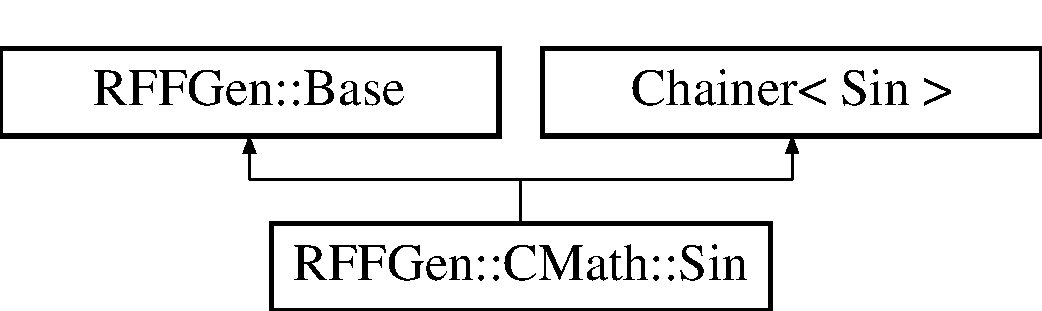
\includegraphics[height=2.000000cm]{structRFFGen_1_1CMath_1_1Sin}
\end{center}
\end{figure}
\subsection*{Public Member Functions}
\begin{DoxyCompactItemize}
\item 
\hyperlink{structRFFGen_1_1CMath_1_1Sin_a5bfac913462b13d50bf31453012201e9}{Sin} (double x=0)
\begin{DoxyCompactList}\small\item\em Constructor. \end{DoxyCompactList}\item 
\hypertarget{structRFFGen_1_1CMath_1_1Sin_af34cc1f856b9588a046e0a52107732a9}{void \hyperlink{structRFFGen_1_1CMath_1_1Sin_af34cc1f856b9588a046e0a52107732a9}{update} (double x)}\label{structRFFGen_1_1CMath_1_1Sin_af34cc1f856b9588a046e0a52107732a9}

\begin{DoxyCompactList}\small\item\em Reset point of evaluation. \end{DoxyCompactList}\item 
\hypertarget{structRFFGen_1_1CMath_1_1Sin_aed617f379892d53d05643227e77c0f8d}{double \hyperlink{structRFFGen_1_1CMath_1_1Sin_aed617f379892d53d05643227e77c0f8d}{d0} () const noexcept}\label{structRFFGen_1_1CMath_1_1Sin_aed617f379892d53d05643227e77c0f8d}

\begin{DoxyCompactList}\small\item\em Function value. \end{DoxyCompactList}\item 
\hypertarget{structRFFGen_1_1CMath_1_1Sin_a481b23f2a4f4af29d5b097aa93e54642}{{\footnotesize template$<$int  = -\/1$>$ }\\double \hyperlink{structRFFGen_1_1CMath_1_1Sin_a481b23f2a4f4af29d5b097aa93e54642}{d1} (double dx=1.) const }\label{structRFFGen_1_1CMath_1_1Sin_a481b23f2a4f4af29d5b097aa93e54642}

\begin{DoxyCompactList}\small\item\em First (directional) derivative. \end{DoxyCompactList}\item 
\hypertarget{structRFFGen_1_1CMath_1_1Sin_a64d5c499d9b212649f194ce2a7110b67}{{\footnotesize template$<$int  = -\/1, int  = -\/1$>$ }\\double \hyperlink{structRFFGen_1_1CMath_1_1Sin_a64d5c499d9b212649f194ce2a7110b67}{d2} (double dx=1., double dy=1.) const }\label{structRFFGen_1_1CMath_1_1Sin_a64d5c499d9b212649f194ce2a7110b67}

\begin{DoxyCompactList}\small\item\em Second (directional) derivative. \end{DoxyCompactList}\item 
\hypertarget{structRFFGen_1_1CMath_1_1Sin_a7ecc5687f60bf51f67f17f313db89d78}{{\footnotesize template$<$int  = -\/1, int  = -\/1, int  = -\/1$>$ }\\double \hyperlink{structRFFGen_1_1CMath_1_1Sin_a7ecc5687f60bf51f67f17f313db89d78}{d3} (double dx=1., double dy=1., double dz=1.) const }\label{structRFFGen_1_1CMath_1_1Sin_a7ecc5687f60bf51f67f17f313db89d78}

\begin{DoxyCompactList}\small\item\em Third (directional) derivative. \end{DoxyCompactList}\end{DoxyCompactItemize}


\subsection{Detailed Description}
Sine function including first three derivatives (based on sin(double) in $<$cmath$>$). 

For scalar functions directional derivatives are less interesting. Incorporating this function as building block for more complex functions requires directional derivatives. These occur during applications of the chain rule. 

\subsection{Constructor \& Destructor Documentation}
\hypertarget{structRFFGen_1_1CMath_1_1Sin_a5bfac913462b13d50bf31453012201e9}{\index{R\-F\-F\-Gen\-::\-C\-Math\-::\-Sin@{R\-F\-F\-Gen\-::\-C\-Math\-::\-Sin}!Sin@{Sin}}
\index{Sin@{Sin}!RFFGen::CMath::Sin@{R\-F\-F\-Gen\-::\-C\-Math\-::\-Sin}}
\subsubsection[{Sin}]{\setlength{\rightskip}{0pt plus 5cm}R\-F\-F\-Gen\-::\-C\-Math\-::\-Sin\-::\-Sin (
\begin{DoxyParamCaption}
\item[{double}]{x = {\ttfamily 0}}
\end{DoxyParamCaption}
)\hspace{0.3cm}{\ttfamily [inline]}, {\ttfamily [explicit]}}}\label{structRFFGen_1_1CMath_1_1Sin_a5bfac913462b13d50bf31453012201e9}


Constructor. 


\begin{DoxyParams}{Parameters}
{\em x} & point of evaluation \\
\hline
\end{DoxyParams}


The documentation for this struct was generated from the following file\-:\begin{DoxyCompactItemize}
\item 
R\-F\-F\-Gen/\-C\-Math/sine.\-hh\end{DoxyCompactItemize}

\hypertarget{structRFFGen_1_1MathematicalOperations_1_1Squared}{\section{R\-F\-F\-Gen\-:\-:Mathematical\-Operations\-:\-:Squared$<$ F, class $>$ Struct Template Reference}
\label{structRFFGen_1_1MathematicalOperations_1_1Squared}\index{R\-F\-F\-Gen\-::\-Mathematical\-Operations\-::\-Squared$<$ F, class $>$@{R\-F\-F\-Gen\-::\-Mathematical\-Operations\-::\-Squared$<$ F, class $>$}}
}


Squared function (F must satisfy the requirements of \hyperlink{structRFFGen_1_1Concepts_1_1FunctionConcept}{Concepts\-::\-Function\-Concept}).  




{\ttfamily \#include $<$squared.\-hh$>$}

Inheritance diagram for R\-F\-F\-Gen\-:\-:Mathematical\-Operations\-:\-:Squared$<$ F, class $>$\-:\begin{figure}[H]
\begin{center}
\leavevmode
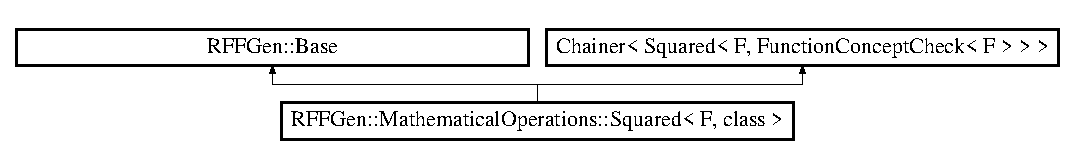
\includegraphics[height=1.421320cm]{structRFFGen_1_1MathematicalOperations_1_1Squared}
\end{center}
\end{figure}
\subsection*{Public Member Functions}
\begin{DoxyCompactItemize}
\item 
\hypertarget{structRFFGen_1_1MathematicalOperations_1_1Squared_a01ac39e60369d635903f4f127fab054e}{\hyperlink{structRFFGen_1_1MathematicalOperations_1_1Squared_a01ac39e60369d635903f4f127fab054e}{Squared} ()=default}\label{structRFFGen_1_1MathematicalOperations_1_1Squared_a01ac39e60369d635903f4f127fab054e}

\begin{DoxyCompactList}\small\item\em Default constructor. May leave member variables uninitialized! Call update before using evaluation. \end{DoxyCompactList}\item 
{\footnotesize template$<$class Init\-F $>$ }\\\hyperlink{structRFFGen_1_1MathematicalOperations_1_1Squared_a8d89d011bdb0456471b02722df029125}{Squared} (const Init\-F \&f\-\_\-)
\begin{DoxyCompactList}\small\item\em Constructor passing arguments to function constructor. \end{DoxyCompactList}\item 
\hypertarget{structRFFGen_1_1MathematicalOperations_1_1Squared_a4b586d514777bd9b670a1c640507cb88}{{\footnotesize template$<$class Arg $>$ }\\void \hyperlink{structRFFGen_1_1MathematicalOperations_1_1Squared_a4b586d514777bd9b670a1c640507cb88}{update} (Arg const \&x)}\label{structRFFGen_1_1MathematicalOperations_1_1Squared_a4b586d514777bd9b670a1c640507cb88}

\begin{DoxyCompactList}\small\item\em Reset point of evaluation. \end{DoxyCompactList}\item 
\hypertarget{structRFFGen_1_1MathematicalOperations_1_1Squared_a2b6d89fb45e7bc60eda730ea1b767b69}{{\footnotesize template$<$int index, class Arg $>$ }\\void \hyperlink{structRFFGen_1_1MathematicalOperations_1_1Squared_a2b6d89fb45e7bc60eda730ea1b767b69}{update\-Variable} (const Arg \&x)}\label{structRFFGen_1_1MathematicalOperations_1_1Squared_a2b6d89fb45e7bc60eda730ea1b767b69}

\begin{DoxyCompactList}\small\item\em Propagate call to \hyperlink{structRFFGen_1_1MathematicalOperations_1_1Squared_a2b6d89fb45e7bc60eda730ea1b767b69}{update\-Variable()} to f. \end{DoxyCompactList}\item 
\hypertarget{structRFFGen_1_1MathematicalOperations_1_1Squared_a2d16f0c33070d97591049e100a76ba68}{const auto \& \hyperlink{structRFFGen_1_1MathematicalOperations_1_1Squared_a2d16f0c33070d97591049e100a76ba68}{d0} () const noexcept}\label{structRFFGen_1_1MathematicalOperations_1_1Squared_a2d16f0c33070d97591049e100a76ba68}

\begin{DoxyCompactList}\small\item\em Function value. \end{DoxyCompactList}\item 
{\footnotesize template$<$int id, class Arg , class Indexed\-Arg  = Indexed\-Type$<$\-Arg,id$>$, class  = std\-::enable\-\_\-if\-\_\-t$<$ Compute\-Product$<$ D0$<$\-F$>$ , D1$<$\-F,\-Indexed\-Arg$>$ $>$\-::present $>$$>$ }\\auto \hyperlink{structRFFGen_1_1MathematicalOperations_1_1Squared_af0f8a775774e5378962fa20e6f909d5d}{d1} (Arg const \&dx) const 
\begin{DoxyCompactList}\small\item\em First directional derivative. \end{DoxyCompactList}\item 
{\footnotesize template$<$int idx, int idy, class Arg\-X , class Arg\-Y , class Indexed\-Arg\-X  = Indexed\-Type$<$\-Arg\-X,idx$>$, class Indexed\-Arg\-Y  = Indexed\-Type$<$\-Arg\-Y,idy$>$, class  = std\-::enable\-\_\-if\-\_\-t$<$ D2\-Sum$<$\-Indexed\-Arg\-X,\-Indexed\-Arg\-Y$>$\-::present $>$$>$ }\\auto \hyperlink{structRFFGen_1_1MathematicalOperations_1_1Squared_a52553adbecffba775c50573e7d478897}{d2} (Arg\-X const \&dx, Arg\-Y const \&dy) const 
\begin{DoxyCompactList}\small\item\em Second directional derivative. \end{DoxyCompactList}\item 
{\footnotesize template$<$int idx, int idy, int idz, class Arg\-X , class Arg\-Y , class Arg\-Z , class Indexed\-Arg\-X  = Indexed\-Type$<$\-Arg\-X,idx$>$, class Indexed\-Arg\-Y  = Indexed\-Type$<$\-Arg\-Y,idy$>$, class Indexed\-Arg\-Z  = Indexed\-Type$<$\-Arg\-Z,idz$>$, class  = std\-::enable\-\_\-if\-\_\-t$<$ D3\-Sum$<$\-Indexed\-Arg\-X,\-Indexed\-Arg\-Y,\-Indexed\-Arg\-Z$>$\-::present $>$$>$ }\\auto \hyperlink{structRFFGen_1_1MathematicalOperations_1_1Squared_ae218404caefa109f0bdf0f94ff9e48e6}{d3} (Arg\-X const \&dx, Arg\-Y const \&dy, Arg\-Z const \&dz) const 
\begin{DoxyCompactList}\small\item\em Third directional derivative. \end{DoxyCompactList}\end{DoxyCompactItemize}


\subsection{Detailed Description}
\subsubsection*{template$<$class F, class = Function\-Concept\-Check$<$\-F$>$$>$struct R\-F\-F\-Gen\-::\-Mathematical\-Operations\-::\-Squared$<$ F, class $>$}

Squared function (F must satisfy the requirements of \hyperlink{structRFFGen_1_1Concepts_1_1FunctionConcept}{Concepts\-::\-Function\-Concept}). 

\subsection{Constructor \& Destructor Documentation}
\hypertarget{structRFFGen_1_1MathematicalOperations_1_1Squared_a8d89d011bdb0456471b02722df029125}{\index{R\-F\-F\-Gen\-::\-Mathematical\-Operations\-::\-Squared@{R\-F\-F\-Gen\-::\-Mathematical\-Operations\-::\-Squared}!Squared@{Squared}}
\index{Squared@{Squared}!RFFGen::MathematicalOperations::Squared@{R\-F\-F\-Gen\-::\-Mathematical\-Operations\-::\-Squared}}
\subsubsection[{Squared}]{\setlength{\rightskip}{0pt plus 5cm}template$<$class F , class  = Function\-Concept\-Check$<$\-F$>$$>$ template$<$class Init\-F $>$ {\bf R\-F\-F\-Gen\-::\-Mathematical\-Operations\-::\-Squared}$<$ F, class $>$\-::{\bf Squared} (
\begin{DoxyParamCaption}
\item[{const Init\-F \&}]{f\-\_\-}
\end{DoxyParamCaption}
)\hspace{0.3cm}{\ttfamily [inline]}}}\label{structRFFGen_1_1MathematicalOperations_1_1Squared_a8d89d011bdb0456471b02722df029125}


Constructor passing arguments to function constructor. 


\begin{DoxyParams}{Parameters}
{\em f\-\_\-} & input for constructor of outer function \\
\hline
\end{DoxyParams}


\subsection{Member Function Documentation}
\hypertarget{structRFFGen_1_1MathematicalOperations_1_1Squared_af0f8a775774e5378962fa20e6f909d5d}{\index{R\-F\-F\-Gen\-::\-Mathematical\-Operations\-::\-Squared@{R\-F\-F\-Gen\-::\-Mathematical\-Operations\-::\-Squared}!d1@{d1}}
\index{d1@{d1}!RFFGen::MathematicalOperations::Squared@{R\-F\-F\-Gen\-::\-Mathematical\-Operations\-::\-Squared}}
\subsubsection[{d1}]{\setlength{\rightskip}{0pt plus 5cm}template$<$class F , class  = Function\-Concept\-Check$<$\-F$>$$>$ template$<$int id, class Arg , class Indexed\-Arg  = Indexed\-Type$<$\-Arg,id$>$, class  = std\-::enable\-\_\-if\-\_\-t$<$ Compute\-Product$<$ D0$<$\-F$>$ , D1$<$\-F,\-Indexed\-Arg$>$ $>$\-::present $>$$>$ auto {\bf R\-F\-F\-Gen\-::\-Mathematical\-Operations\-::\-Squared}$<$ F, class $>$\-::d1 (
\begin{DoxyParamCaption}
\item[{Arg const \&}]{dx}
\end{DoxyParamCaption}
) const\hspace{0.3cm}{\ttfamily [inline]}}}\label{structRFFGen_1_1MathematicalOperations_1_1Squared_af0f8a775774e5378962fa20e6f909d5d}


First directional derivative. 


\begin{DoxyParams}{Parameters}
{\em dx} & direction for which the derivative is computed \\
\hline
\end{DoxyParams}
\hypertarget{structRFFGen_1_1MathematicalOperations_1_1Squared_a52553adbecffba775c50573e7d478897}{\index{R\-F\-F\-Gen\-::\-Mathematical\-Operations\-::\-Squared@{R\-F\-F\-Gen\-::\-Mathematical\-Operations\-::\-Squared}!d2@{d2}}
\index{d2@{d2}!RFFGen::MathematicalOperations::Squared@{R\-F\-F\-Gen\-::\-Mathematical\-Operations\-::\-Squared}}
\subsubsection[{d2}]{\setlength{\rightskip}{0pt plus 5cm}template$<$class F , class  = Function\-Concept\-Check$<$\-F$>$$>$ template$<$int idx, int idy, class Arg\-X , class Arg\-Y , class Indexed\-Arg\-X  = Indexed\-Type$<$\-Arg\-X,idx$>$, class Indexed\-Arg\-Y  = Indexed\-Type$<$\-Arg\-Y,idy$>$, class  = std\-::enable\-\_\-if\-\_\-t$<$ D2\-Sum$<$\-Indexed\-Arg\-X,\-Indexed\-Arg\-Y$>$\-::present $>$$>$ auto {\bf R\-F\-F\-Gen\-::\-Mathematical\-Operations\-::\-Squared}$<$ F, class $>$\-::d2 (
\begin{DoxyParamCaption}
\item[{Arg\-X const \&}]{dx, }
\item[{Arg\-Y const \&}]{dy}
\end{DoxyParamCaption}
) const\hspace{0.3cm}{\ttfamily [inline]}}}\label{structRFFGen_1_1MathematicalOperations_1_1Squared_a52553adbecffba775c50573e7d478897}


Second directional derivative. 


\begin{DoxyParams}{Parameters}
{\em dx} & direction for which the derivative is computed \\
\hline
{\em dy} & direction for which the derivative is computed \\
\hline
\end{DoxyParams}
\hypertarget{structRFFGen_1_1MathematicalOperations_1_1Squared_ae218404caefa109f0bdf0f94ff9e48e6}{\index{R\-F\-F\-Gen\-::\-Mathematical\-Operations\-::\-Squared@{R\-F\-F\-Gen\-::\-Mathematical\-Operations\-::\-Squared}!d3@{d3}}
\index{d3@{d3}!RFFGen::MathematicalOperations::Squared@{R\-F\-F\-Gen\-::\-Mathematical\-Operations\-::\-Squared}}
\subsubsection[{d3}]{\setlength{\rightskip}{0pt plus 5cm}template$<$class F , class  = Function\-Concept\-Check$<$\-F$>$$>$ template$<$int idx, int idy, int idz, class Arg\-X , class Arg\-Y , class Arg\-Z , class Indexed\-Arg\-X  = Indexed\-Type$<$\-Arg\-X,idx$>$, class Indexed\-Arg\-Y  = Indexed\-Type$<$\-Arg\-Y,idy$>$, class Indexed\-Arg\-Z  = Indexed\-Type$<$\-Arg\-Z,idz$>$, class  = std\-::enable\-\_\-if\-\_\-t$<$ D3\-Sum$<$\-Indexed\-Arg\-X,\-Indexed\-Arg\-Y,\-Indexed\-Arg\-Z$>$\-::present $>$$>$ auto {\bf R\-F\-F\-Gen\-::\-Mathematical\-Operations\-::\-Squared}$<$ F, class $>$\-::d3 (
\begin{DoxyParamCaption}
\item[{Arg\-X const \&}]{dx, }
\item[{Arg\-Y const \&}]{dy, }
\item[{Arg\-Z const \&}]{dz}
\end{DoxyParamCaption}
) const\hspace{0.3cm}{\ttfamily [inline]}}}\label{structRFFGen_1_1MathematicalOperations_1_1Squared_ae218404caefa109f0bdf0f94ff9e48e6}


Third directional derivative. 


\begin{DoxyParams}{Parameters}
{\em dx} & direction for which the derivative is computed \\
\hline
{\em dy} & direction for which the derivative is computed \\
\hline
{\em dz} & direction for which the derivative is computed \\
\hline
\end{DoxyParams}


The documentation for this struct was generated from the following file\-:\begin{DoxyCompactItemize}
\item 
R\-F\-F\-Gen/\-Mathematical\-Operations/squared.\-hh\end{DoxyCompactItemize}

\hypertarget{structRFFGen_1_1LinearAlgebra_1_1SquaredEuclideanNorm}{\section{R\-F\-F\-Gen\-:\-:Linear\-Algebra\-:\-:Squared\-Euclidean\-Norm$<$ Matrix, class $>$ Struct Template Reference}
\label{structRFFGen_1_1LinearAlgebra_1_1SquaredEuclideanNorm}\index{R\-F\-F\-Gen\-::\-Linear\-Algebra\-::\-Squared\-Euclidean\-Norm$<$ Matrix, class $>$@{R\-F\-F\-Gen\-::\-Linear\-Algebra\-::\-Squared\-Euclidean\-Norm$<$ Matrix, class $>$}}
}


Compute squared matrix norm $ \|A\|^2 = A\negthinspace : \negthinspace A = \mathrm{tr}(A^TA) = \sum_{i,j} A_{ij}^2. $.  




{\ttfamily \#include $<$euclidean\-Norm.\-hh$>$}

Inheritance diagram for R\-F\-F\-Gen\-:\-:Linear\-Algebra\-:\-:Squared\-Euclidean\-Norm$<$ Matrix, class $>$\-:\begin{figure}[H]
\begin{center}
\leavevmode
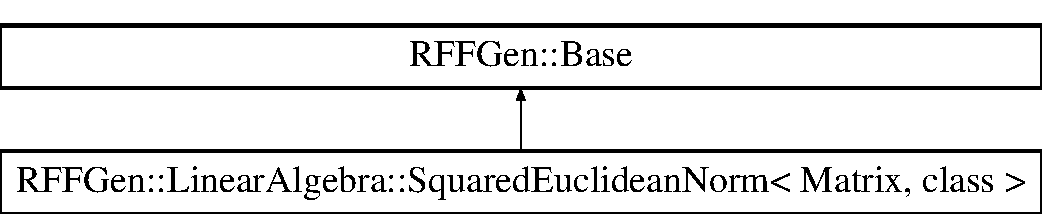
\includegraphics[height=2.000000cm]{structRFFGen_1_1LinearAlgebra_1_1SquaredEuclideanNorm}
\end{center}
\end{figure}
\subsection*{Public Member Functions}
\begin{DoxyCompactItemize}
\item 
\hypertarget{structRFFGen_1_1LinearAlgebra_1_1SquaredEuclideanNorm_ac18eccb286a23ab1b27f38ad44a9edf7}{\hyperlink{structRFFGen_1_1LinearAlgebra_1_1SquaredEuclideanNorm_ac18eccb286a23ab1b27f38ad44a9edf7}{Squared\-Euclidean\-Norm} ()=default}\label{structRFFGen_1_1LinearAlgebra_1_1SquaredEuclideanNorm_ac18eccb286a23ab1b27f38ad44a9edf7}

\begin{DoxyCompactList}\small\item\em Default constructor. \end{DoxyCompactList}\item 
\hyperlink{structRFFGen_1_1LinearAlgebra_1_1SquaredEuclideanNorm_a5d87d3db87bd84795b36b99634db6971}{Squared\-Euclidean\-Norm} (const Matrix \&A)
\begin{DoxyCompactList}\small\item\em Constructor. \end{DoxyCompactList}\item 
\hypertarget{structRFFGen_1_1LinearAlgebra_1_1SquaredEuclideanNorm_a1bde9f1d59eccf58dca3775d95ed1d65}{void \hyperlink{structRFFGen_1_1LinearAlgebra_1_1SquaredEuclideanNorm_a1bde9f1d59eccf58dca3775d95ed1d65}{update} (const Matrix \&A)}\label{structRFFGen_1_1LinearAlgebra_1_1SquaredEuclideanNorm_a1bde9f1d59eccf58dca3775d95ed1d65}

\begin{DoxyCompactList}\small\item\em Reset matrix to compute squared norm from. \end{DoxyCompactList}\item 
\hypertarget{structRFFGen_1_1LinearAlgebra_1_1SquaredEuclideanNorm_aed33c87d01510cb61ed6579f03c4a08d}{auto \hyperlink{structRFFGen_1_1LinearAlgebra_1_1SquaredEuclideanNorm_aed33c87d01510cb61ed6579f03c4a08d}{operator()} () const noexcept}\label{structRFFGen_1_1LinearAlgebra_1_1SquaredEuclideanNorm_aed33c87d01510cb61ed6579f03c4a08d}

\begin{DoxyCompactList}\small\item\em Squared matrix norm. Convenient access to \hyperlink{structRFFGen_1_1LinearAlgebra_1_1SquaredEuclideanNorm_a837bc49a8a0d090a14f402c0f04d06ed}{d0()}. \end{DoxyCompactList}\item 
\hypertarget{structRFFGen_1_1LinearAlgebra_1_1SquaredEuclideanNorm_a837bc49a8a0d090a14f402c0f04d06ed}{auto \hyperlink{structRFFGen_1_1LinearAlgebra_1_1SquaredEuclideanNorm_a837bc49a8a0d090a14f402c0f04d06ed}{d0} () const noexcept}\label{structRFFGen_1_1LinearAlgebra_1_1SquaredEuclideanNorm_a837bc49a8a0d090a14f402c0f04d06ed}

\begin{DoxyCompactList}\small\item\em Squared matrix norm. \end{DoxyCompactList}\item 
\hypertarget{structRFFGen_1_1LinearAlgebra_1_1SquaredEuclideanNorm_a64dc292d1da02c39d08f379e5082cb12}{{\footnotesize template$<$int $>$ }\\auto \hyperlink{structRFFGen_1_1LinearAlgebra_1_1SquaredEuclideanNorm_a64dc292d1da02c39d08f379e5082cb12}{d1} (const Matrix \&d\-A) const }\label{structRFFGen_1_1LinearAlgebra_1_1SquaredEuclideanNorm_a64dc292d1da02c39d08f379e5082cb12}

\begin{DoxyCompactList}\small\item\em First directional derivative. \end{DoxyCompactList}\item 
\hypertarget{structRFFGen_1_1LinearAlgebra_1_1SquaredEuclideanNorm_abdff448da2b743ec46fb07127b237dbc}{{\footnotesize template$<$int , int $>$ }\\auto \hyperlink{structRFFGen_1_1LinearAlgebra_1_1SquaredEuclideanNorm_abdff448da2b743ec46fb07127b237dbc}{d2} (const Matrix \&d\-A1, const Matrix \&d\-A2) const }\label{structRFFGen_1_1LinearAlgebra_1_1SquaredEuclideanNorm_abdff448da2b743ec46fb07127b237dbc}

\begin{DoxyCompactList}\small\item\em Second directional derivative. \end{DoxyCompactList}\end{DoxyCompactItemize}


\subsection{Detailed Description}
\subsubsection*{template$<$class Matrix, class = Concepts\-::\-Matrix\-Concept\-Check$<$\-Matrix$>$$>$struct R\-F\-F\-Gen\-::\-Linear\-Algebra\-::\-Squared\-Euclidean\-Norm$<$ Matrix, class $>$}

Compute squared matrix norm $ \|A\|^2 = A\negthinspace : \negthinspace A = \mathrm{tr}(A^TA) = \sum_{i,j} A_{ij}^2. $. 

\subsection{Constructor \& Destructor Documentation}
\hypertarget{structRFFGen_1_1LinearAlgebra_1_1SquaredEuclideanNorm_a5d87d3db87bd84795b36b99634db6971}{\index{R\-F\-F\-Gen\-::\-Linear\-Algebra\-::\-Squared\-Euclidean\-Norm@{R\-F\-F\-Gen\-::\-Linear\-Algebra\-::\-Squared\-Euclidean\-Norm}!Squared\-Euclidean\-Norm@{Squared\-Euclidean\-Norm}}
\index{Squared\-Euclidean\-Norm@{Squared\-Euclidean\-Norm}!RFFGen::LinearAlgebra::SquaredEuclideanNorm@{R\-F\-F\-Gen\-::\-Linear\-Algebra\-::\-Squared\-Euclidean\-Norm}}
\subsubsection[{Squared\-Euclidean\-Norm}]{\setlength{\rightskip}{0pt plus 5cm}template$<$class Matrix , class  = Concepts\-::\-Matrix\-Concept\-Check$<$\-Matrix$>$$>$ {\bf R\-F\-F\-Gen\-::\-Linear\-Algebra\-::\-Squared\-Euclidean\-Norm}$<$ Matrix, class $>$\-::{\bf Squared\-Euclidean\-Norm} (
\begin{DoxyParamCaption}
\item[{const Matrix \&}]{A}
\end{DoxyParamCaption}
)\hspace{0.3cm}{\ttfamily [inline]}, {\ttfamily [explicit]}}}\label{structRFFGen_1_1LinearAlgebra_1_1SquaredEuclideanNorm_a5d87d3db87bd84795b36b99634db6971}


Constructor. 


\begin{DoxyParams}{Parameters}
{\em A} & matrix to compute squared norm from. \\
\hline
\end{DoxyParams}


The documentation for this struct was generated from the following file\-:\begin{DoxyCompactItemize}
\item 
R\-F\-F\-Gen/\-Linear\-Algebra/euclidean\-Norm.\-hh\end{DoxyCompactItemize}

\hypertarget{structRFFGen_1_1LinearAlgebra_1_1SquaredMatrixNorm}{\section{R\-F\-F\-Gen\-:\-:Linear\-Algebra\-:\-:Squared\-Matrix\-Norm$<$ Matrix, class $>$ Struct Template Reference}
\label{structRFFGen_1_1LinearAlgebra_1_1SquaredMatrixNorm}\index{R\-F\-F\-Gen\-::\-Linear\-Algebra\-::\-Squared\-Matrix\-Norm$<$ Matrix, class $>$@{R\-F\-F\-Gen\-::\-Linear\-Algebra\-::\-Squared\-Matrix\-Norm$<$ Matrix, class $>$}}
}


Compute squared matrix norm $ \|A\|^2 = A\negthinspace : \negthinspace A = \mathrm{tr}(A^TA) = \sum_{i,j} A_{ij}^2. $.  




{\ttfamily \#include $<$matrix\-Norm.\-hh$>$}

Inheritance diagram for R\-F\-F\-Gen\-:\-:Linear\-Algebra\-:\-:Squared\-Matrix\-Norm$<$ Matrix, class $>$\-:\begin{figure}[H]
\begin{center}
\leavevmode
\includegraphics[height=2.000000cm]{structRFFGen_1_1LinearAlgebra_1_1SquaredMatrixNorm}
\end{center}
\end{figure}
\subsection*{Public Member Functions}
\begin{DoxyCompactItemize}
\item 
\hypertarget{structRFFGen_1_1LinearAlgebra_1_1SquaredMatrixNorm_a12a675f8253661fb62915ba3f6f2d6e6}{\hyperlink{structRFFGen_1_1LinearAlgebra_1_1SquaredMatrixNorm_a12a675f8253661fb62915ba3f6f2d6e6}{Squared\-Matrix\-Norm} ()=default}\label{structRFFGen_1_1LinearAlgebra_1_1SquaredMatrixNorm_a12a675f8253661fb62915ba3f6f2d6e6}

\begin{DoxyCompactList}\small\item\em Default constructor. \end{DoxyCompactList}\item 
\hyperlink{structRFFGen_1_1LinearAlgebra_1_1SquaredMatrixNorm_a32420aa809b04ad2ce2f72f6e93de2f3}{Squared\-Matrix\-Norm} (const Matrix \&A)
\begin{DoxyCompactList}\small\item\em Constructor. \end{DoxyCompactList}\item 
\hypertarget{structRFFGen_1_1LinearAlgebra_1_1SquaredMatrixNorm_a3b7bbeb2d36bea1117a551c8d168c4d6}{void \hyperlink{structRFFGen_1_1LinearAlgebra_1_1SquaredMatrixNorm_a3b7bbeb2d36bea1117a551c8d168c4d6}{update} (const Matrix \&A)}\label{structRFFGen_1_1LinearAlgebra_1_1SquaredMatrixNorm_a3b7bbeb2d36bea1117a551c8d168c4d6}

\begin{DoxyCompactList}\small\item\em Reset matrix to compute squared norm from. \end{DoxyCompactList}\item 
\hypertarget{structRFFGen_1_1LinearAlgebra_1_1SquaredMatrixNorm_a6aee4181a9dfb2a146f2cee3cca6a562}{auto \hyperlink{structRFFGen_1_1LinearAlgebra_1_1SquaredMatrixNorm_a6aee4181a9dfb2a146f2cee3cca6a562}{operator()} () const noexcept}\label{structRFFGen_1_1LinearAlgebra_1_1SquaredMatrixNorm_a6aee4181a9dfb2a146f2cee3cca6a562}

\begin{DoxyCompactList}\small\item\em Squared matrix norm. Convenient access to \hyperlink{structRFFGen_1_1LinearAlgebra_1_1SquaredMatrixNorm_abaa6151eafb9baefe973bd313920c92c}{d0()}. \end{DoxyCompactList}\item 
\hypertarget{structRFFGen_1_1LinearAlgebra_1_1SquaredMatrixNorm_abaa6151eafb9baefe973bd313920c92c}{auto \hyperlink{structRFFGen_1_1LinearAlgebra_1_1SquaredMatrixNorm_abaa6151eafb9baefe973bd313920c92c}{d0} () const noexcept}\label{structRFFGen_1_1LinearAlgebra_1_1SquaredMatrixNorm_abaa6151eafb9baefe973bd313920c92c}

\begin{DoxyCompactList}\small\item\em Squared matrix norm. \end{DoxyCompactList}\item 
\hypertarget{structRFFGen_1_1LinearAlgebra_1_1SquaredMatrixNorm_ae27b37478ba3e246f73d8383e11c1f84}{{\footnotesize template$<$int $>$ }\\auto \hyperlink{structRFFGen_1_1LinearAlgebra_1_1SquaredMatrixNorm_ae27b37478ba3e246f73d8383e11c1f84}{d1} (const Matrix \&d\-A) const }\label{structRFFGen_1_1LinearAlgebra_1_1SquaredMatrixNorm_ae27b37478ba3e246f73d8383e11c1f84}

\begin{DoxyCompactList}\small\item\em First directional derivative. \end{DoxyCompactList}\item 
\hypertarget{structRFFGen_1_1LinearAlgebra_1_1SquaredMatrixNorm_aaf6162ac724beec933f9f531e2a353f1}{{\footnotesize template$<$int , int $>$ }\\auto \hyperlink{structRFFGen_1_1LinearAlgebra_1_1SquaredMatrixNorm_aaf6162ac724beec933f9f531e2a353f1}{d2} (const Matrix \&d\-A1, const Matrix \&d\-A2) const }\label{structRFFGen_1_1LinearAlgebra_1_1SquaredMatrixNorm_aaf6162ac724beec933f9f531e2a353f1}

\begin{DoxyCompactList}\small\item\em Second directional derivative. \end{DoxyCompactList}\end{DoxyCompactItemize}


\subsection{Detailed Description}
\subsubsection*{template$<$class Matrix, class = Concepts\-::\-Matrix\-Concept\-Check$<$\-Matrix$>$$>$struct R\-F\-F\-Gen\-::\-Linear\-Algebra\-::\-Squared\-Matrix\-Norm$<$ Matrix, class $>$}

Compute squared matrix norm $ \|A\|^2 = A\negthinspace : \negthinspace A = \mathrm{tr}(A^TA) = \sum_{i,j} A_{ij}^2. $. 

\subsection{Constructor \& Destructor Documentation}
\hypertarget{structRFFGen_1_1LinearAlgebra_1_1SquaredMatrixNorm_a32420aa809b04ad2ce2f72f6e93de2f3}{\index{R\-F\-F\-Gen\-::\-Linear\-Algebra\-::\-Squared\-Matrix\-Norm@{R\-F\-F\-Gen\-::\-Linear\-Algebra\-::\-Squared\-Matrix\-Norm}!Squared\-Matrix\-Norm@{Squared\-Matrix\-Norm}}
\index{Squared\-Matrix\-Norm@{Squared\-Matrix\-Norm}!RFFGen::LinearAlgebra::SquaredMatrixNorm@{R\-F\-F\-Gen\-::\-Linear\-Algebra\-::\-Squared\-Matrix\-Norm}}
\subsubsection[{Squared\-Matrix\-Norm}]{\setlength{\rightskip}{0pt plus 5cm}template$<$class Matrix , class  = Concepts\-::\-Matrix\-Concept\-Check$<$\-Matrix$>$$>$ {\bf R\-F\-F\-Gen\-::\-Linear\-Algebra\-::\-Squared\-Matrix\-Norm}$<$ Matrix, class $>$\-::{\bf Squared\-Matrix\-Norm} (
\begin{DoxyParamCaption}
\item[{const Matrix \&}]{A}
\end{DoxyParamCaption}
)\hspace{0.3cm}{\ttfamily [inline]}, {\ttfamily [explicit]}}}\label{structRFFGen_1_1LinearAlgebra_1_1SquaredMatrixNorm_a32420aa809b04ad2ce2f72f6e93de2f3}


Constructor. 


\begin{DoxyParams}{Parameters}
{\em A} & matrix to compute squared norm from. \\
\hline
\end{DoxyParams}


The documentation for this struct was generated from the following file\-:\begin{DoxyCompactItemize}
\item 
R\-F\-F\-Gen/\-Linear\-Algebra/matrix\-Norm.\-hh\end{DoxyCompactItemize}

\hypertarget{classRFFGen_1_1LinearAlgebra_1_1StrainTensor}{\section{R\-F\-F\-Gen\-:\-:Linear\-Algebra\-:\-:Strain\-Tensor$<$ Matrix $>$ Class Template Reference}
\label{classRFFGen_1_1LinearAlgebra_1_1StrainTensor}\index{R\-F\-F\-Gen\-::\-Linear\-Algebra\-::\-Strain\-Tensor$<$ Matrix $>$@{R\-F\-F\-Gen\-::\-Linear\-Algebra\-::\-Strain\-Tensor$<$ Matrix $>$}}
}


Strain tensor $ \frac{1}{2}\left(F^T+F\right + F^T F) $.  




{\ttfamily \#include $<$strain\-Tensor.\-hh$>$}

Inheritance diagram for R\-F\-F\-Gen\-:\-:Linear\-Algebra\-:\-:Strain\-Tensor$<$ Matrix $>$\-:\begin{figure}[H]
\begin{center}
\leavevmode
\includegraphics[height=1.733746cm]{classRFFGen_1_1LinearAlgebra_1_1StrainTensor}
\end{center}
\end{figure}
\subsection*{Public Member Functions}
\begin{DoxyCompactItemize}
\item 
\hyperlink{classRFFGen_1_1LinearAlgebra_1_1StrainTensor_afc03693af7fd7515cd0073db840af715}{Strain\-Tensor} (const Matrix \&F)
\begin{DoxyCompactList}\small\item\em Constructor. \end{DoxyCompactList}\end{DoxyCompactItemize}


\subsection{Detailed Description}
\subsubsection*{template$<$class Matrix$>$class R\-F\-F\-Gen\-::\-Linear\-Algebra\-::\-Strain\-Tensor$<$ Matrix $>$}

Strain tensor $ \frac{1}{2}\left(F^T+F\right + F^T F) $. 

This class is used for nonlinear material models based on the displacement gradient $\nabla u$, which takes the role of $F$. Implemented as Sum$<$\-Linearized\-Strain\-Tensor,\-Geometric\-Nonlinearity$>$. 

\subsection{Constructor \& Destructor Documentation}
\hypertarget{classRFFGen_1_1LinearAlgebra_1_1StrainTensor_afc03693af7fd7515cd0073db840af715}{\index{R\-F\-F\-Gen\-::\-Linear\-Algebra\-::\-Strain\-Tensor@{R\-F\-F\-Gen\-::\-Linear\-Algebra\-::\-Strain\-Tensor}!Strain\-Tensor@{Strain\-Tensor}}
\index{Strain\-Tensor@{Strain\-Tensor}!RFFGen::LinearAlgebra::StrainTensor@{R\-F\-F\-Gen\-::\-Linear\-Algebra\-::\-Strain\-Tensor}}
\subsubsection[{Strain\-Tensor}]{\setlength{\rightskip}{0pt plus 5cm}template$<$class Matrix $>$ {\bf R\-F\-F\-Gen\-::\-Linear\-Algebra\-::\-Strain\-Tensor}$<$ Matrix $>$\-::{\bf Strain\-Tensor} (
\begin{DoxyParamCaption}
\item[{const Matrix \&}]{F}
\end{DoxyParamCaption}
)\hspace{0.3cm}{\ttfamily [inline]}, {\ttfamily [explicit]}}}\label{classRFFGen_1_1LinearAlgebra_1_1StrainTensor_afc03693af7fd7515cd0073db840af715}


Constructor. 


\begin{DoxyParams}{Parameters}
{\em F} & point of evaluation \\
\hline
\end{DoxyParams}


The documentation for this class was generated from the following file\-:\begin{DoxyCompactItemize}
\item 
R\-F\-F\-Gen/\-Linear\-Algebra/strain\-Tensor.\-hh\end{DoxyCompactItemize}

\hypertarget{structRFFGen_1_1MathematicalOperations_1_1Sum}{\section{R\-F\-F\-Gen\-:\-:Mathematical\-Operations\-:\-:Sum$<$ F, G, Check\-F, Check\-G $>$ Struct Template Reference}
\label{structRFFGen_1_1MathematicalOperations_1_1Sum}\index{R\-F\-F\-Gen\-::\-Mathematical\-Operations\-::\-Sum$<$ F, G, Check\-F, Check\-G $>$@{R\-F\-F\-Gen\-::\-Mathematical\-Operations\-::\-Sum$<$ F, G, Check\-F, Check\-G $>$}}
}


Sum of functions of type F and G (F and G must satisfy the requirements of \hyperlink{structRFFGen_1_1Concepts_1_1FunctionConcept}{Concepts\-::\-Function\-Concept}).  




{\ttfamily \#include $<$sum.\-hh$>$}

Inheritance diagram for R\-F\-F\-Gen\-:\-:Mathematical\-Operations\-:\-:Sum$<$ F, G, Check\-F, Check\-G $>$\-:\begin{figure}[H]
\begin{center}
\leavevmode
\includegraphics[height=1.414141cm]{structRFFGen_1_1MathematicalOperations_1_1Sum}
\end{center}
\end{figure}
\subsection*{Public Member Functions}
\begin{DoxyCompactItemize}
\item 
{\footnotesize template$<$class Init\-F , class Init\-G $>$ }\\\hyperlink{structRFFGen_1_1MathematicalOperations_1_1Sum_a8abfebcfef4096f4838fdf49bfbb998a}{Sum} (const Init\-F \&f\-\_\-, const Init\-G \&g\-\_\-)
\begin{DoxyCompactList}\small\item\em Constructor passing arguments to function constructors. \end{DoxyCompactList}\item 
\hypertarget{structRFFGen_1_1MathematicalOperations_1_1Sum_a10c688bb03d5de23728aea547205307b}{{\footnotesize template$<$class Arg $>$ }\\void \hyperlink{structRFFGen_1_1MathematicalOperations_1_1Sum_a10c688bb03d5de23728aea547205307b}{update} (Arg const \&x)}\label{structRFFGen_1_1MathematicalOperations_1_1Sum_a10c688bb03d5de23728aea547205307b}

\begin{DoxyCompactList}\small\item\em Reset point of evaluation. \end{DoxyCompactList}\item 
\hypertarget{structRFFGen_1_1MathematicalOperations_1_1Sum_a6ca0cb2a7c64ee03125f0babcd8ca13a}{{\footnotesize template$<$int index, class Arg $>$ }\\void \hyperlink{structRFFGen_1_1MathematicalOperations_1_1Sum_a6ca0cb2a7c64ee03125f0babcd8ca13a}{update\-Variable} (const Arg \&x)}\label{structRFFGen_1_1MathematicalOperations_1_1Sum_a6ca0cb2a7c64ee03125f0babcd8ca13a}

\begin{DoxyCompactList}\small\item\em Propagate call to \hyperlink{structRFFGen_1_1MathematicalOperations_1_1Sum_a6ca0cb2a7c64ee03125f0babcd8ca13a}{update\-Variable()} to f and g. \end{DoxyCompactList}\item 
\hypertarget{structRFFGen_1_1MathematicalOperations_1_1Sum_ab253acf4c0ee66164c51bf7b3bb6bc85}{const auto \& \hyperlink{structRFFGen_1_1MathematicalOperations_1_1Sum_ab253acf4c0ee66164c51bf7b3bb6bc85}{d0} () const noexcept}\label{structRFFGen_1_1MathematicalOperations_1_1Sum_ab253acf4c0ee66164c51bf7b3bb6bc85}

\begin{DoxyCompactList}\small\item\em Function value. \end{DoxyCompactList}\item 
{\footnotesize template$<$int id, class Arg , class Indexed\-Arg  = Indexed\-Type$<$\-Arg,id$>$, class  = std\-::enable\-\_\-if\-\_\-t$<$ Compute\-Sum$<$ D1$<$\-F,\-Indexed\-Arg$>$, D1$<$\-G,\-Indexed\-Arg$>$ $>$\-::present $>$$>$ }\\auto \hyperlink{structRFFGen_1_1MathematicalOperations_1_1Sum_a10c105fc333d2663a28699bcba0b087a}{d1} (const Arg \&dx) const 
\begin{DoxyCompactList}\small\item\em First directional derivative. \end{DoxyCompactList}\item 
{\footnotesize template$<$int idx, int idy, class Arg\-X , class Arg\-Y , class Indexed\-Arg\-X  = Indexed\-Type$<$\-Arg\-X,idx$>$, class Indexed\-Arg\-Y  = Indexed\-Type$<$\-Arg\-Y,idy$>$, class  = std\-::enable\-\_\-if\-\_\-t$<$ Compute\-Sum$<$ D2$<$\-F,\-Indexed\-Arg\-X,\-Indexed\-Arg\-Y$>$, D2$<$\-G,\-Indexed\-Arg\-X,\-Indexed\-Arg\-Y$>$ $>$\-::present $>$$>$ }\\auto \hyperlink{structRFFGen_1_1MathematicalOperations_1_1Sum_a227ae4c1437e245f9a25199fb03c0f08}{d2} (const Arg\-X \&dx, const Arg\-Y \&dy) const 
\begin{DoxyCompactList}\small\item\em Second directional derivative. \end{DoxyCompactList}\item 
{\footnotesize template$<$int idx, int idy, int idz, class Arg\-X , class Arg\-Y , class Arg\-Z , class Indexed\-Arg\-X  = Indexed\-Type$<$\-Arg\-X,idx$>$, class Indexed\-Arg\-Y  = Indexed\-Type$<$\-Arg\-Y,idy$>$, class Indexed\-Arg\-Z  = Indexed\-Type$<$\-Arg\-Z,idz$>$, class  = std\-::enable\-\_\-if\-\_\-t$<$ Compute\-Sum$<$ D3$<$\-F,\-Indexed\-Arg\-X,\-Indexed\-Arg\-Y,\-Indexed\-Arg\-Z$>$, D3$<$\-G,\-Indexed\-Arg\-X,\-Indexed\-Arg\-Y,\-Indexed\-Arg\-Z$>$ $>$\-::present $>$$>$ }\\auto \hyperlink{structRFFGen_1_1MathematicalOperations_1_1Sum_a797e6bd471d4bc155fb710e78272c313}{d3} (const Arg\-X \&dx, const Arg\-Y \&dy, const Arg\-Z \&dz) const 
\begin{DoxyCompactList}\small\item\em Third directional derivative. \end{DoxyCompactList}\end{DoxyCompactItemize}


\subsection{Detailed Description}
\subsubsection*{template$<$class F, class G, class Check\-F = Function\-Concept\-Check$<$\-F$>$, class Check\-G = Function\-Concept\-Check$<$\-G$>$$>$struct R\-F\-F\-Gen\-::\-Mathematical\-Operations\-::\-Sum$<$ F, G, Check\-F, Check\-G $>$}

Sum of functions of type F and G (F and G must satisfy the requirements of \hyperlink{structRFFGen_1_1Concepts_1_1FunctionConcept}{Concepts\-::\-Function\-Concept}). 

\subsection{Constructor \& Destructor Documentation}
\hypertarget{structRFFGen_1_1MathematicalOperations_1_1Sum_a8abfebcfef4096f4838fdf49bfbb998a}{\index{R\-F\-F\-Gen\-::\-Mathematical\-Operations\-::\-Sum@{R\-F\-F\-Gen\-::\-Mathematical\-Operations\-::\-Sum}!Sum@{Sum}}
\index{Sum@{Sum}!RFFGen::MathematicalOperations::Sum@{R\-F\-F\-Gen\-::\-Mathematical\-Operations\-::\-Sum}}
\subsubsection[{Sum}]{\setlength{\rightskip}{0pt plus 5cm}template$<$class F, class G, class Check\-F = Function\-Concept\-Check$<$\-F$>$, class Check\-G = Function\-Concept\-Check$<$\-G$>$$>$ template$<$class Init\-F , class Init\-G $>$ {\bf R\-F\-F\-Gen\-::\-Mathematical\-Operations\-::\-Sum}$<$ F, G, Check\-F, Check\-G $>$\-::{\bf Sum} (
\begin{DoxyParamCaption}
\item[{const Init\-F \&}]{f\-\_\-, }
\item[{const Init\-G \&}]{g\-\_\-}
\end{DoxyParamCaption}
)\hspace{0.3cm}{\ttfamily [inline]}}}\label{structRFFGen_1_1MathematicalOperations_1_1Sum_a8abfebcfef4096f4838fdf49bfbb998a}


Constructor passing arguments to function constructors. 


\begin{DoxyParams}{Parameters}
{\em f\-\_\-} & input for constructor of first summand \\
\hline
{\em g\-\_\-} & input for constructor of second summand \\
\hline
\end{DoxyParams}


\subsection{Member Function Documentation}
\hypertarget{structRFFGen_1_1MathematicalOperations_1_1Sum_a10c105fc333d2663a28699bcba0b087a}{\index{R\-F\-F\-Gen\-::\-Mathematical\-Operations\-::\-Sum@{R\-F\-F\-Gen\-::\-Mathematical\-Operations\-::\-Sum}!d1@{d1}}
\index{d1@{d1}!RFFGen::MathematicalOperations::Sum@{R\-F\-F\-Gen\-::\-Mathematical\-Operations\-::\-Sum}}
\subsubsection[{d1}]{\setlength{\rightskip}{0pt plus 5cm}template$<$class F, class G, class Check\-F = Function\-Concept\-Check$<$\-F$>$, class Check\-G = Function\-Concept\-Check$<$\-G$>$$>$ template$<$int id, class Arg , class Indexed\-Arg  = Indexed\-Type$<$\-Arg,id$>$, class  = std\-::enable\-\_\-if\-\_\-t$<$ Compute\-Sum$<$ D1$<$\-F,\-Indexed\-Arg$>$, D1$<$\-G,\-Indexed\-Arg$>$ $>$\-::present $>$$>$ auto {\bf R\-F\-F\-Gen\-::\-Mathematical\-Operations\-::\-Sum}$<$ F, G, Check\-F, Check\-G $>$\-::d1 (
\begin{DoxyParamCaption}
\item[{const Arg \&}]{dx}
\end{DoxyParamCaption}
) const\hspace{0.3cm}{\ttfamily [inline]}}}\label{structRFFGen_1_1MathematicalOperations_1_1Sum_a10c105fc333d2663a28699bcba0b087a}


First directional derivative. 


\begin{DoxyParams}{Parameters}
{\em dx} & direction for which the derivative is computed \\
\hline
\end{DoxyParams}
\hypertarget{structRFFGen_1_1MathematicalOperations_1_1Sum_a227ae4c1437e245f9a25199fb03c0f08}{\index{R\-F\-F\-Gen\-::\-Mathematical\-Operations\-::\-Sum@{R\-F\-F\-Gen\-::\-Mathematical\-Operations\-::\-Sum}!d2@{d2}}
\index{d2@{d2}!RFFGen::MathematicalOperations::Sum@{R\-F\-F\-Gen\-::\-Mathematical\-Operations\-::\-Sum}}
\subsubsection[{d2}]{\setlength{\rightskip}{0pt plus 5cm}template$<$class F, class G, class Check\-F = Function\-Concept\-Check$<$\-F$>$, class Check\-G = Function\-Concept\-Check$<$\-G$>$$>$ template$<$int idx, int idy, class Arg\-X , class Arg\-Y , class Indexed\-Arg\-X  = Indexed\-Type$<$\-Arg\-X,idx$>$, class Indexed\-Arg\-Y  = Indexed\-Type$<$\-Arg\-Y,idy$>$, class  = std\-::enable\-\_\-if\-\_\-t$<$ Compute\-Sum$<$ D2$<$\-F,\-Indexed\-Arg\-X,\-Indexed\-Arg\-Y$>$, D2$<$\-G,\-Indexed\-Arg\-X,\-Indexed\-Arg\-Y$>$ $>$\-::present $>$$>$ auto {\bf R\-F\-F\-Gen\-::\-Mathematical\-Operations\-::\-Sum}$<$ F, G, Check\-F, Check\-G $>$\-::d2 (
\begin{DoxyParamCaption}
\item[{const Arg\-X \&}]{dx, }
\item[{const Arg\-Y \&}]{dy}
\end{DoxyParamCaption}
) const\hspace{0.3cm}{\ttfamily [inline]}}}\label{structRFFGen_1_1MathematicalOperations_1_1Sum_a227ae4c1437e245f9a25199fb03c0f08}


Second directional derivative. 


\begin{DoxyParams}{Parameters}
{\em dx} & direction for which the derivative is computed \\
\hline
{\em dy} & direction for which the derivative is computed \\
\hline
\end{DoxyParams}
\hypertarget{structRFFGen_1_1MathematicalOperations_1_1Sum_a797e6bd471d4bc155fb710e78272c313}{\index{R\-F\-F\-Gen\-::\-Mathematical\-Operations\-::\-Sum@{R\-F\-F\-Gen\-::\-Mathematical\-Operations\-::\-Sum}!d3@{d3}}
\index{d3@{d3}!RFFGen::MathematicalOperations::Sum@{R\-F\-F\-Gen\-::\-Mathematical\-Operations\-::\-Sum}}
\subsubsection[{d3}]{\setlength{\rightskip}{0pt plus 5cm}template$<$class F, class G, class Check\-F = Function\-Concept\-Check$<$\-F$>$, class Check\-G = Function\-Concept\-Check$<$\-G$>$$>$ template$<$int idx, int idy, int idz, class Arg\-X , class Arg\-Y , class Arg\-Z , class Indexed\-Arg\-X  = Indexed\-Type$<$\-Arg\-X,idx$>$, class Indexed\-Arg\-Y  = Indexed\-Type$<$\-Arg\-Y,idy$>$, class Indexed\-Arg\-Z  = Indexed\-Type$<$\-Arg\-Z,idz$>$, class  = std\-::enable\-\_\-if\-\_\-t$<$ Compute\-Sum$<$ D3$<$\-F,\-Indexed\-Arg\-X,\-Indexed\-Arg\-Y,\-Indexed\-Arg\-Z$>$, D3$<$\-G,\-Indexed\-Arg\-X,\-Indexed\-Arg\-Y,\-Indexed\-Arg\-Z$>$ $>$\-::present $>$$>$ auto {\bf R\-F\-F\-Gen\-::\-Mathematical\-Operations\-::\-Sum}$<$ F, G, Check\-F, Check\-G $>$\-::d3 (
\begin{DoxyParamCaption}
\item[{const Arg\-X \&}]{dx, }
\item[{const Arg\-Y \&}]{dy, }
\item[{const Arg\-Z \&}]{dz}
\end{DoxyParamCaption}
) const\hspace{0.3cm}{\ttfamily [inline]}}}\label{structRFFGen_1_1MathematicalOperations_1_1Sum_a797e6bd471d4bc155fb710e78272c313}


Third directional derivative. 


\begin{DoxyParams}{Parameters}
{\em dx} & direction for which the derivative is computed \\
\hline
{\em dy} & direction for which the derivative is computed \\
\hline
{\em dz} & direction for which the derivative is computed \\
\hline
\end{DoxyParams}


The documentation for this struct was generated from the following file\-:\begin{DoxyCompactItemize}
\item 
R\-F\-F\-Gen/\-Mathematical\-Operations/sum.\-hh\end{DoxyCompactItemize}

\hypertarget{structRFFGen_1_1Concepts_1_1SummationConcept}{\section{R\-F\-F\-Gen\-:\-:Concepts\-:\-:Summation\-Concept Struct Reference}
\label{structRFFGen_1_1Concepts_1_1SummationConcept}\index{R\-F\-F\-Gen\-::\-Concepts\-::\-Summation\-Concept@{R\-F\-F\-Gen\-::\-Concepts\-::\-Summation\-Concept}}
}


Requires that summation can be performed either by in-\/place summation or free summation.  




{\ttfamily \#include $<$concepts.\-hh$>$}

Inheritance diagram for R\-F\-F\-Gen\-:\-:Concepts\-:\-:Summation\-Concept\-:\begin{figure}[H]
\begin{center}
\leavevmode
\includegraphics[height=2.058824cm]{structRFFGen_1_1Concepts_1_1SummationConcept}
\end{center}
\end{figure}
\subsection*{Public Member Functions}
\begin{DoxyCompactItemize}
\item 
\hypertarget{structRFFGen_1_1Concepts_1_1SummationConcept_adc0349034311b99726f0c845d8c06a33}{unspecified \hyperlink{structRFFGen_1_1Concepts_1_1SummationConcept_adc0349034311b99726f0c845d8c06a33}{operator+=} (\hyperlink{structRFFGen_1_1Concepts_1_1SummationConcept}{Summation\-Concept})}\label{structRFFGen_1_1Concepts_1_1SummationConcept_adc0349034311b99726f0c845d8c06a33}

\begin{DoxyCompactList}\small\item\em In-\/place summation. Return type is not checked to support lazy evaluation. \end{DoxyCompactList}\end{DoxyCompactItemize}


\subsection{Detailed Description}
Requires that summation can be performed either by in-\/place summation or free summation. 

The documentation for this struct was generated from the following file\-:\begin{DoxyCompactItemize}
\item 
R\-F\-F\-Gen/\hyperlink{concepts_8hh}{concepts.\-hh}\end{DoxyCompactItemize}

\hypertarget{structRFFGen_1_1Concepts_1_1SummationConceptCheck}{\section{R\-F\-F\-Gen\-:\-:Concepts\-:\-:Summation\-Concept\-Check$<$ Arg $>$ Struct Template Reference}
\label{structRFFGen_1_1Concepts_1_1SummationConceptCheck}\index{R\-F\-F\-Gen\-::\-Concepts\-::\-Summation\-Concept\-Check$<$ Arg $>$@{R\-F\-F\-Gen\-::\-Concepts\-::\-Summation\-Concept\-Check$<$ Arg $>$}}
}


Static check if the requirements of \hyperlink{structRFFGen_1_1Concepts_1_1SummationConcept}{Summation\-Concept} are satisfied.  




{\ttfamily \#include $<$concept\-Check.\-hh$>$}

Inheritance diagram for R\-F\-F\-Gen\-:\-:Concepts\-:\-:Summation\-Concept\-Check$<$ Arg $>$\-:\begin{figure}[H]
\begin{center}
\leavevmode
\includegraphics[height=2.000000cm]{structRFFGen_1_1Concepts_1_1SummationConceptCheck}
\end{center}
\end{figure}


\subsection{Detailed Description}
\subsubsection*{template$<$class Arg$>$struct R\-F\-F\-Gen\-::\-Concepts\-::\-Summation\-Concept\-Check$<$ Arg $>$}

Static check if the requirements of \hyperlink{structRFFGen_1_1Concepts_1_1SummationConcept}{Summation\-Concept} are satisfied. 


\begin{DoxyTemplParams}{Template Parameters}
{\em Arg} & type to check \\
\hline
\end{DoxyTemplParams}


The documentation for this struct was generated from the following file\-:\begin{DoxyCompactItemize}
\item 
R\-F\-F\-Gen/concept\-Check.\-hh\end{DoxyCompactItemize}

\hypertarget{structRFFGen_1_1Concepts_1_1SymmetricMatrixConcept}{\section{R\-F\-F\-Gen\-:\-:Concepts\-:\-:Symmetric\-Matrix\-Concept Struct Reference}
\label{structRFFGen_1_1Concepts_1_1SymmetricMatrixConcept}\index{R\-F\-F\-Gen\-::\-Concepts\-::\-Symmetric\-Matrix\-Concept@{R\-F\-F\-Gen\-::\-Concepts\-::\-Symmetric\-Matrix\-Concept}}
}


Requirements for symmetric matrices.  




{\ttfamily \#include $<$concepts.\-hh$>$}

Inheritance diagram for R\-F\-F\-Gen\-:\-:Concepts\-:\-:Symmetric\-Matrix\-Concept\-:\begin{figure}[H]
\begin{center}
\leavevmode
\includegraphics[height=1.586402cm]{structRFFGen_1_1Concepts_1_1SymmetricMatrixConcept}
\end{center}
\end{figure}
\subsection*{Additional Inherited Members}


\subsection{Detailed Description}
Requirements for symmetric matrices. 

The requirements of \hyperlink{structRFFGen_1_1Concepts_1_1MatrixConcept}{Matrix\-Concept} must be satisfied and the number of rows and columns must be equal. 

The documentation for this struct was generated from the following file\-:\begin{DoxyCompactItemize}
\item 
R\-F\-F\-Gen/\hyperlink{concepts_8hh}{concepts.\-hh}\end{DoxyCompactItemize}

\hypertarget{structRFFGen_1_1Concepts_1_1SymmetricMatrixConceptCheck}{\section{R\-F\-F\-Gen\-:\-:Concepts\-:\-:Symmetric\-Matrix\-Concept\-Check$<$ Matrix $>$ Struct Template Reference}
\label{structRFFGen_1_1Concepts_1_1SymmetricMatrixConceptCheck}\index{R\-F\-F\-Gen\-::\-Concepts\-::\-Symmetric\-Matrix\-Concept\-Check$<$ Matrix $>$@{R\-F\-F\-Gen\-::\-Concepts\-::\-Symmetric\-Matrix\-Concept\-Check$<$ Matrix $>$}}
}


Static check if the requirements of \hyperlink{structRFFGen_1_1Concepts_1_1SymmetricMatrixConcept}{Symmetric\-Matrix\-Concept} are satisfied.  




{\ttfamily \#include $<$concept\-Check.\-hh$>$}

Inheritance diagram for R\-F\-F\-Gen\-:\-:Concepts\-:\-:Symmetric\-Matrix\-Concept\-Check$<$ Matrix $>$\-:\begin{figure}[H]
\begin{center}
\leavevmode
\includegraphics[height=1.666667cm]{structRFFGen_1_1Concepts_1_1SymmetricMatrixConceptCheck}
\end{center}
\end{figure}


\subsection{Detailed Description}
\subsubsection*{template$<$class Matrix$>$struct R\-F\-F\-Gen\-::\-Concepts\-::\-Symmetric\-Matrix\-Concept\-Check$<$ Matrix $>$}

Static check if the requirements of \hyperlink{structRFFGen_1_1Concepts_1_1SymmetricMatrixConcept}{Symmetric\-Matrix\-Concept} are satisfied. 

The documentation for this struct was generated from the following file\-:\begin{DoxyCompactItemize}
\item 
R\-F\-F\-Gen/concept\-Check.\-hh\end{DoxyCompactItemize}

\hypertarget{structRFFGen_1_1CMath_1_1Tan}{\section{R\-F\-F\-Gen\-:\-:C\-Math\-:\-:Tan Struct Reference}
\label{structRFFGen_1_1CMath_1_1Tan}\index{R\-F\-F\-Gen\-::\-C\-Math\-::\-Tan@{R\-F\-F\-Gen\-::\-C\-Math\-::\-Tan}}
}


Tangent function including first three derivatives.  




{\ttfamily \#include $<$tan.\-hh$>$}

Inheritance diagram for R\-F\-F\-Gen\-:\-:C\-Math\-:\-:Tan\-:\begin{figure}[H]
\begin{center}
\leavevmode
\includegraphics[height=2.000000cm]{structRFFGen_1_1CMath_1_1Tan}
\end{center}
\end{figure}
\subsection*{Public Member Functions}
\begin{DoxyCompactItemize}
\item 
\hyperlink{structRFFGen_1_1CMath_1_1Tan_aab69e654f41b935e2b769f8e707da514}{Tan} (double x=0.)
\begin{DoxyCompactList}\small\item\em Constructor. \end{DoxyCompactList}\item 
\hypertarget{structRFFGen_1_1CMath_1_1Tan_ab77126a0316332722070fc4186f8498a}{void \hyperlink{structRFFGen_1_1CMath_1_1Tan_ab77126a0316332722070fc4186f8498a}{update} (double x)}\label{structRFFGen_1_1CMath_1_1Tan_ab77126a0316332722070fc4186f8498a}

\begin{DoxyCompactList}\small\item\em Reset point of evaluation. \end{DoxyCompactList}\item 
\hypertarget{structRFFGen_1_1CMath_1_1Tan_a302990b9cf78bc9657c6ebde39bc9313}{double \hyperlink{structRFFGen_1_1CMath_1_1Tan_a302990b9cf78bc9657c6ebde39bc9313}{d0} () const noexcept}\label{structRFFGen_1_1CMath_1_1Tan_a302990b9cf78bc9657c6ebde39bc9313}

\begin{DoxyCompactList}\small\item\em Function value. \end{DoxyCompactList}\item 
\hypertarget{structRFFGen_1_1CMath_1_1Tan_a6910c6ef9d204385ab3a3be99f927f95}{{\footnotesize template$<$int  = -\/1$>$ }\\double \hyperlink{structRFFGen_1_1CMath_1_1Tan_a6910c6ef9d204385ab3a3be99f927f95}{d1} (double dx=1.) const }\label{structRFFGen_1_1CMath_1_1Tan_a6910c6ef9d204385ab3a3be99f927f95}

\begin{DoxyCompactList}\small\item\em First (directional) derivative. \end{DoxyCompactList}\item 
\hypertarget{structRFFGen_1_1CMath_1_1Tan_a4d5229c3c812cc8f0d43f67a4aeee1e0}{{\footnotesize template$<$int  = -\/1, int  = -\/1$>$ }\\double \hyperlink{structRFFGen_1_1CMath_1_1Tan_a4d5229c3c812cc8f0d43f67a4aeee1e0}{d2} (double dx=1., double dy=1.) const }\label{structRFFGen_1_1CMath_1_1Tan_a4d5229c3c812cc8f0d43f67a4aeee1e0}

\begin{DoxyCompactList}\small\item\em Second (directinal) derivative. \end{DoxyCompactList}\item 
\hypertarget{structRFFGen_1_1CMath_1_1Tan_ad0263de083e6ade627a8ffe638805b3f}{{\footnotesize template$<$int  = -\/1, int  = -\/1, int  = -\/1$>$ }\\double \hyperlink{structRFFGen_1_1CMath_1_1Tan_ad0263de083e6ade627a8ffe638805b3f}{d3} (double dx=1., double dy=1., double dz=1.) const }\label{structRFFGen_1_1CMath_1_1Tan_ad0263de083e6ade627a8ffe638805b3f}

\begin{DoxyCompactList}\small\item\em Third (directional) derivative. \end{DoxyCompactList}\end{DoxyCompactItemize}


\subsection{Detailed Description}
Tangent function including first three derivatives. 

For scalar functions directional derivatives are less interesting. Incorporating this function as building block for more complex functions requires directional derivatives. These occur during applications of the chain rule. 

\subsection{Constructor \& Destructor Documentation}
\hypertarget{structRFFGen_1_1CMath_1_1Tan_aab69e654f41b935e2b769f8e707da514}{\index{R\-F\-F\-Gen\-::\-C\-Math\-::\-Tan@{R\-F\-F\-Gen\-::\-C\-Math\-::\-Tan}!Tan@{Tan}}
\index{Tan@{Tan}!RFFGen::CMath::Tan@{R\-F\-F\-Gen\-::\-C\-Math\-::\-Tan}}
\subsubsection[{Tan}]{\setlength{\rightskip}{0pt plus 5cm}R\-F\-F\-Gen\-::\-C\-Math\-::\-Tan\-::\-Tan (
\begin{DoxyParamCaption}
\item[{double}]{x = {\ttfamily 0.}}
\end{DoxyParamCaption}
)\hspace{0.3cm}{\ttfamily [inline]}, {\ttfamily [explicit]}}}\label{structRFFGen_1_1CMath_1_1Tan_aab69e654f41b935e2b769f8e707da514}


Constructor. 


\begin{DoxyParams}{Parameters}
{\em x} & point of evaluation \\
\hline
\end{DoxyParams}


The documentation for this struct was generated from the following file\-:\begin{DoxyCompactItemize}
\item 
R\-F\-F\-Gen/\-C\-Math/tan.\-hh\end{DoxyCompactItemize}

\hypertarget{structRFFGen_1_1LinearAlgebra_1_1ThirdModifiedMixedInvariant}{\section{R\-F\-F\-Gen\-:\-:Linear\-Algebra\-:\-:Third\-Modified\-Mixed\-Invariant$<$ Matrix, class $>$ Struct Template Reference}
\label{structRFFGen_1_1LinearAlgebra_1_1ThirdModifiedMixedInvariant}\index{R\-F\-F\-Gen\-::\-Linear\-Algebra\-::\-Third\-Modified\-Mixed\-Invariant$<$ Matrix, class $>$@{R\-F\-F\-Gen\-::\-Linear\-Algebra\-::\-Third\-Modified\-Mixed\-Invariant$<$ Matrix, class $>$}}
}


Third modified mixed invariant $\bar\iota_6=\iota_6\iota_3^{-1/3}$.  




{\ttfamily \#include $<$modified\-Mixed\-Invariants.\-hh$>$}

Inheritance diagram for R\-F\-F\-Gen\-:\-:Linear\-Algebra\-:\-:Third\-Modified\-Mixed\-Invariant$<$ Matrix, class $>$\-:\begin{figure}[H]
\begin{center}
\leavevmode
\includegraphics[height=2.000000cm]{structRFFGen_1_1LinearAlgebra_1_1ThirdModifiedMixedInvariant}
\end{center}
\end{figure}
\subsection*{Public Member Functions}
\begin{DoxyCompactItemize}
\item 
\hypertarget{structRFFGen_1_1LinearAlgebra_1_1ThirdModifiedMixedInvariant_a1739098d1de2ffbdaa0f148e9d1adba1}{\hyperlink{structRFFGen_1_1LinearAlgebra_1_1ThirdModifiedMixedInvariant_a1739098d1de2ffbdaa0f148e9d1adba1}{Third\-Modified\-Mixed\-Invariant} ()=default}\label{structRFFGen_1_1LinearAlgebra_1_1ThirdModifiedMixedInvariant_a1739098d1de2ffbdaa0f148e9d1adba1}

\begin{DoxyCompactList}\small\item\em Default constructor. \end{DoxyCompactList}\item 
\hyperlink{structRFFGen_1_1LinearAlgebra_1_1ThirdModifiedMixedInvariant_aea5e2e2d814d5bfe7f483ba6ea4bfd1d}{Third\-Modified\-Mixed\-Invariant} (const Matrix \&A, const \hyperlink{structRFFGen_1_1Constant}{Constant}$<$ Matrix $>$ \&M)
\begin{DoxyCompactList}\small\item\em Constructor. \end{DoxyCompactList}\end{DoxyCompactItemize}


\subsection{Detailed Description}
\subsubsection*{template$<$class Matrix, class = Concepts\-::\-Symmetric\-Matrix\-Concept\-Check$<$\-Matrix$>$$>$struct R\-F\-F\-Gen\-::\-Linear\-Algebra\-::\-Third\-Modified\-Mixed\-Invariant$<$ Matrix, class $>$}

Third modified mixed invariant $\bar\iota_6=\iota_6\iota_3^{-1/3}$. 

\subsection{Constructor \& Destructor Documentation}
\hypertarget{structRFFGen_1_1LinearAlgebra_1_1ThirdModifiedMixedInvariant_aea5e2e2d814d5bfe7f483ba6ea4bfd1d}{\index{R\-F\-F\-Gen\-::\-Linear\-Algebra\-::\-Third\-Modified\-Mixed\-Invariant@{R\-F\-F\-Gen\-::\-Linear\-Algebra\-::\-Third\-Modified\-Mixed\-Invariant}!Third\-Modified\-Mixed\-Invariant@{Third\-Modified\-Mixed\-Invariant}}
\index{Third\-Modified\-Mixed\-Invariant@{Third\-Modified\-Mixed\-Invariant}!RFFGen::LinearAlgebra::ThirdModifiedMixedInvariant@{R\-F\-F\-Gen\-::\-Linear\-Algebra\-::\-Third\-Modified\-Mixed\-Invariant}}
\subsubsection[{Third\-Modified\-Mixed\-Invariant}]{\setlength{\rightskip}{0pt plus 5cm}template$<$class Matrix , class  = Concepts\-::\-Symmetric\-Matrix\-Concept\-Check$<$\-Matrix$>$$>$ {\bf R\-F\-F\-Gen\-::\-Linear\-Algebra\-::\-Third\-Modified\-Mixed\-Invariant}$<$ Matrix, class $>$\-::{\bf Third\-Modified\-Mixed\-Invariant} (
\begin{DoxyParamCaption}
\item[{const Matrix \&}]{A, }
\item[{const {\bf Constant}$<$ Matrix $>$ \&}]{M}
\end{DoxyParamCaption}
)\hspace{0.3cm}{\ttfamily [inline]}}}\label{structRFFGen_1_1LinearAlgebra_1_1ThirdModifiedMixedInvariant_aea5e2e2d814d5bfe7f483ba6ea4bfd1d}


Constructor. 


\begin{DoxyParams}{Parameters}
{\em A} & matrix to compute third modified mixed invariant from. \\
\hline
{\em M} & structural tensor incorporating anisotropic information. \\
\hline
\end{DoxyParams}


The documentation for this struct was generated from the following file\-:\begin{DoxyCompactItemize}
\item 
R\-F\-F\-Gen/\-Linear\-Algebra/modified\-Mixed\-Invariants.\-hh\end{DoxyCompactItemize}

\hypertarget{structRFFGen_1_1Variable}{\section{R\-F\-F\-Gen\-:\-:Variable$<$ T, id $>$ Struct Template Reference}
\label{structRFFGen_1_1Variable}\index{R\-F\-F\-Gen\-::\-Variable$<$ T, id $>$@{R\-F\-F\-Gen\-::\-Variable$<$ T, id $>$}}
}


Independent variable. Can be uniquely identified by its id.  




{\ttfamily \#include $<$variable.\-hh$>$}

Inheritance diagram for R\-F\-F\-Gen\-:\-:Variable$<$ T, id $>$\-:\begin{figure}[H]
\begin{center}
\leavevmode
\includegraphics[height=2.000000cm]{structRFFGen_1_1Variable}
\end{center}
\end{figure}
\subsection*{Public Member Functions}
\begin{DoxyCompactItemize}
\item 
\hypertarget{structRFFGen_1_1Variable_a99bcfbe635b7a9c221d6ba3bb068921d}{\hyperlink{structRFFGen_1_1Variable_a99bcfbe635b7a9c221d6ba3bb068921d}{Variable} (const T \&t\-\_\-)}\label{structRFFGen_1_1Variable_a99bcfbe635b7a9c221d6ba3bb068921d}

\begin{DoxyCompactList}\small\item\em Construct variable with meaningful default value. \end{DoxyCompactList}\item 
\hypertarget{structRFFGen_1_1Variable_a5d6591b5a95842811ce015bbc98d8cb1}{{\footnotesize template$<$int index, class Arg $>$ }\\void \hyperlink{structRFFGen_1_1Variable_a5d6591b5a95842811ce015bbc98d8cb1}{update\-Variable} (const Arg \&t\-\_\-)}\label{structRFFGen_1_1Variable_a5d6591b5a95842811ce015bbc98d8cb1}

\begin{DoxyCompactList}\small\item\em Update variable. \end{DoxyCompactList}\item 
\hypertarget{structRFFGen_1_1Variable_af9705f9ea1deb1066db0edd317e12ec4}{const T \& \hyperlink{structRFFGen_1_1Variable_af9705f9ea1deb1066db0edd317e12ec4}{operator()} () const noexcept}\label{structRFFGen_1_1Variable_af9705f9ea1deb1066db0edd317e12ec4}

\begin{DoxyCompactList}\small\item\em Value of the variable. Convenient access to \hyperlink{structRFFGen_1_1Variable_abab2ca1e85b626e4bb656b97f899de74}{d0()}. \end{DoxyCompactList}\item 
\hypertarget{structRFFGen_1_1Variable_abab2ca1e85b626e4bb656b97f899de74}{const T \& \hyperlink{structRFFGen_1_1Variable_abab2ca1e85b626e4bb656b97f899de74}{d0} () const noexcept}\label{structRFFGen_1_1Variable_abab2ca1e85b626e4bb656b97f899de74}

\begin{DoxyCompactList}\small\item\em Value of the variable. \end{DoxyCompactList}\item 
{\footnotesize template$<$int index, class  = std\-::enable\-\_\-if\-\_\-t$<$ id == index $>$$>$ }\\const T \& \hyperlink{structRFFGen_1_1Variable_a7950779c766f047ead4baa03ebaca3bc}{d1} (const T \&dt) const noexcept
\begin{DoxyCompactList}\small\item\em First directional derivative. \end{DoxyCompactList}\end{DoxyCompactItemize}


\subsection{Detailed Description}
\subsubsection*{template$<$class T, int id$>$struct R\-F\-F\-Gen\-::\-Variable$<$ T, id $>$}

Independent variable. Can be uniquely identified by its id. 

\subsection{Member Function Documentation}
\hypertarget{structRFFGen_1_1Variable_a7950779c766f047ead4baa03ebaca3bc}{\index{R\-F\-F\-Gen\-::\-Variable@{R\-F\-F\-Gen\-::\-Variable}!d1@{d1}}
\index{d1@{d1}!RFFGen::Variable@{R\-F\-F\-Gen\-::\-Variable}}
\subsubsection[{d1}]{\setlength{\rightskip}{0pt plus 5cm}template$<$class T , int id$>$ template$<$int index, class  = std\-::enable\-\_\-if\-\_\-t$<$ id == index $>$$>$ const T\& {\bf R\-F\-F\-Gen\-::\-Variable}$<$ T, id $>$\-::d1 (
\begin{DoxyParamCaption}
\item[{const T \&}]{dt}
\end{DoxyParamCaption}
) const\hspace{0.3cm}{\ttfamily [inline]}, {\ttfamily [noexcept]}}}\label{structRFFGen_1_1Variable_a7950779c766f047ead4baa03ebaca3bc}


First directional derivative. 

Only available if id==index. 

The documentation for this struct was generated from the following file\-:\begin{DoxyCompactItemize}
\item 
R\-F\-F\-Gen/variable.\-hh\end{DoxyCompactItemize}

\hypertarget{structRFFGen_1_1Concepts_1_1VectorConcept}{\section{R\-F\-F\-Gen\-:\-:Concepts\-:\-:Vector\-Concept Struct Reference}
\label{structRFFGen_1_1Concepts_1_1VectorConcept}\index{R\-F\-F\-Gen\-::\-Concepts\-::\-Vector\-Concept@{R\-F\-F\-Gen\-::\-Concepts\-::\-Vector\-Concept}}
}


Requirements for vectors.  




{\ttfamily \#include $<$concepts.\-hh$>$}

Inheritance diagram for R\-F\-F\-Gen\-:\-:Concepts\-:\-:Vector\-Concept\-:\begin{figure}[H]
\begin{center}
\leavevmode
\includegraphics[height=1.586402cm]{structRFFGen_1_1Concepts_1_1VectorConcept}
\end{center}
\end{figure}
\subsection*{Public Member Functions}
\begin{DoxyCompactItemize}
\item 
\hypertarget{structRFFGen_1_1Concepts_1_1VectorConcept_ae3c1eba9ae7c1789b0261b9c75b45451}{unspecified \hyperlink{structRFFGen_1_1Concepts_1_1VectorConcept_ae3c1eba9ae7c1789b0261b9c75b45451}{operator\mbox{[}$\,$\mbox{]}} (int)}\label{structRFFGen_1_1Concepts_1_1VectorConcept_ae3c1eba9ae7c1789b0261b9c75b45451}

\begin{DoxyCompactList}\small\item\em Access to entry. \end{DoxyCompactList}\item 
\hypertarget{structRFFGen_1_1Concepts_1_1VectorConcept_a1922a4ed887026d05dfc511132d8d0cb}{unspecified \hyperlink{structRFFGen_1_1Concepts_1_1VectorConcept_a1922a4ed887026d05dfc511132d8d0cb}{operator()} (int)}\label{structRFFGen_1_1Concepts_1_1VectorConcept_a1922a4ed887026d05dfc511132d8d0cb}

\begin{DoxyCompactList}\small\item\em Access to entry. \end{DoxyCompactList}\end{DoxyCompactItemize}


\subsection{Detailed Description}
Requirements for vectors. 

Access to vector elements must be possible either via A\mbox{[}i\mbox{]} or A(i). Moreover the requirements of \hyperlink{structRFFGen_1_1Concepts_1_1ArithmeticConcept}{Arithmetic\-Concept} must be satisfied. 

The documentation for this struct was generated from the following file\-:\begin{DoxyCompactItemize}
\item 
R\-F\-F\-Gen/\hyperlink{concepts_8hh}{concepts.\-hh}\end{DoxyCompactItemize}

\hypertarget{structRFFGen_1_1Concepts_1_1VectorConceptCheck}{\section{R\-F\-F\-Gen\-:\-:Concepts\-:\-:Vector\-Concept\-Check$<$ Vector $>$ Struct Template Reference}
\label{structRFFGen_1_1Concepts_1_1VectorConceptCheck}\index{R\-F\-F\-Gen\-::\-Concepts\-::\-Vector\-Concept\-Check$<$ Vector $>$@{R\-F\-F\-Gen\-::\-Concepts\-::\-Vector\-Concept\-Check$<$ Vector $>$}}
}


Static check if the requirements of \hyperlink{structRFFGen_1_1Concepts_1_1VectorConcept}{Vector\-Concept} are satisfied.  




{\ttfamily \#include $<$concept\-Check.\-hh$>$}

Inheritance diagram for R\-F\-F\-Gen\-:\-:Concepts\-:\-:Vector\-Concept\-Check$<$ Vector $>$\-:\begin{figure}[H]
\begin{center}
\leavevmode
\includegraphics[height=1.241685cm]{structRFFGen_1_1Concepts_1_1VectorConceptCheck}
\end{center}
\end{figure}


\subsection{Detailed Description}
\subsubsection*{template$<$class Vector$>$struct R\-F\-F\-Gen\-::\-Concepts\-::\-Vector\-Concept\-Check$<$ Vector $>$}

Static check if the requirements of \hyperlink{structRFFGen_1_1Concepts_1_1VectorConcept}{Vector\-Concept} are satisfied. 

The documentation for this struct was generated from the following file\-:\begin{DoxyCompactItemize}
\item 
R\-F\-F\-Gen/concept\-Check.\-hh\end{DoxyCompactItemize}

\hypertarget{structRFFGen_1_1YieldSurface}{\section{R\-F\-F\-Gen\-:\-:Yield\-Surface$<$ Matrix $>$ Struct Template Reference}
\label{structRFFGen_1_1YieldSurface}\index{R\-F\-F\-Gen\-::\-Yield\-Surface$<$ Matrix $>$@{R\-F\-F\-Gen\-::\-Yield\-Surface$<$ Matrix $>$}}
}


Yield surface $ \frac{\beta}{3}\iota_1(\sigma) + J_2(\sigma)-offset $, where $\iota_1$ is the first principal and $J_2$ is the second deviatoric invariant.  




{\ttfamily \#include $<$yield\-Surface.\-hh$>$}

Inheritance diagram for R\-F\-F\-Gen\-:\-:Yield\-Surface$<$ Matrix $>$\-:\begin{figure}[H]
\begin{center}
\leavevmode
\includegraphics[height=2.000000cm]{structRFFGen_1_1YieldSurface}
\end{center}
\end{figure}
\subsection*{Public Member Functions}
\begin{DoxyCompactItemize}
\item 
\hyperlink{structRFFGen_1_1YieldSurface_a061091a108035834b402c4f6ad7a1085}{Yield\-Surface} (double beta, double offset, Matrix sigma=unit\-Matrix$<$ Matrix $>$())
\begin{DoxyCompactList}\small\item\em Constructor. \end{DoxyCompactList}\end{DoxyCompactItemize}


\subsection{Detailed Description}
\subsubsection*{template$<$class Matrix$>$struct R\-F\-F\-Gen\-::\-Yield\-Surface$<$ Matrix $>$}

Yield surface $ \frac{\beta}{3}\iota_1(\sigma) + J_2(\sigma)-offset $, where $\iota_1$ is the first principal and $J_2$ is the second deviatoric invariant. 

\subsection{Constructor \& Destructor Documentation}
\hypertarget{structRFFGen_1_1YieldSurface_a061091a108035834b402c4f6ad7a1085}{\index{R\-F\-F\-Gen\-::\-Yield\-Surface@{R\-F\-F\-Gen\-::\-Yield\-Surface}!Yield\-Surface@{Yield\-Surface}}
\index{Yield\-Surface@{Yield\-Surface}!RFFGen::YieldSurface@{R\-F\-F\-Gen\-::\-Yield\-Surface}}
\subsubsection[{Yield\-Surface}]{\setlength{\rightskip}{0pt plus 5cm}template$<$class Matrix $>$ {\bf R\-F\-F\-Gen\-::\-Yield\-Surface}$<$ Matrix $>$\-::{\bf Yield\-Surface} (
\begin{DoxyParamCaption}
\item[{double}]{beta, }
\item[{double}]{offset, }
\item[{Matrix}]{sigma = {\ttfamily unitMatrix$<$Matrix$>$()}}
\end{DoxyParamCaption}
)\hspace{0.3cm}{\ttfamily [inline]}, {\ttfamily [explicit]}}}\label{structRFFGen_1_1YieldSurface_a061091a108035834b402c4f6ad7a1085}


Constructor. 


\begin{DoxyParams}{Parameters}
{\em beta} & scaling \\
\hline
{\em offset} & offset \\
\hline
{\em sigma} & stress tensor \\
\hline
\end{DoxyParams}


The documentation for this struct was generated from the following file\-:\begin{DoxyCompactItemize}
\item 
R\-F\-F\-Gen/\-Examples/yield\-Surface.\-hh\end{DoxyCompactItemize}

\hypertarget{structRFFGen_1_1Zero}{\section{R\-F\-F\-Gen\-:\-:Zero$<$ Matrix, class $>$ Struct Template Reference}
\label{structRFFGen_1_1Zero}\index{R\-F\-F\-Gen\-::\-Zero$<$ Matrix, class $>$@{R\-F\-F\-Gen\-::\-Zero$<$ Matrix, class $>$}}
}


Specialize this struct for your matrix type if a zero matrix cannot be generated via Matrix(0.).  




{\ttfamily \#include $<$zero.\-hh$>$}

\subsection*{Public Member Functions}
\begin{DoxyCompactItemize}
\item 
Matrix \hyperlink{structRFFGen_1_1Zero_ad3cf2a2228843b69537b5fc67c95c43f}{operator()} () const 
\end{DoxyCompactItemize}


\subsection{Detailed Description}
\subsubsection*{template$<$class Matrix, class = void$>$struct R\-F\-F\-Gen\-::\-Zero$<$ Matrix, class $>$}

Specialize this struct for your matrix type if a zero matrix cannot be generated via Matrix(0.). 

\subsection{Member Function Documentation}
\hypertarget{structRFFGen_1_1Zero_ad3cf2a2228843b69537b5fc67c95c43f}{\index{R\-F\-F\-Gen\-::\-Zero@{R\-F\-F\-Gen\-::\-Zero}!operator()@{operator()}}
\index{operator()@{operator()}!RFFGen::Zero@{R\-F\-F\-Gen\-::\-Zero}}
\subsubsection[{operator()}]{\setlength{\rightskip}{0pt plus 5cm}template$<$class Matrix , class  = void$>$ Matrix {\bf R\-F\-F\-Gen\-::\-Zero}$<$ Matrix, class $>$\-::operator() (
\begin{DoxyParamCaption}
{}
\end{DoxyParamCaption}
) const\hspace{0.3cm}{\ttfamily [inline]}}}\label{structRFFGen_1_1Zero_ad3cf2a2228843b69537b5fc67c95c43f}
\begin{DoxyReturn}{Returns}
zero matrix 
\end{DoxyReturn}


The documentation for this struct was generated from the following file\-:\begin{DoxyCompactItemize}
\item 
R\-F\-F\-Gen/\-Util/zero.\-hh\end{DoxyCompactItemize}

\hypertarget{structRFFGen_1_1Zero_3_01Matrix_00_01void__t_3_01Checks_1_1TryCallToZeroes_3_01Matrix_01_4_01_4_01_4}{\section{R\-F\-F\-Gen\-:\-:Zero$<$ Matrix, void\-\_\-t$<$ Checks\-:\-:Try\-Call\-To\-Zeroes$<$ Matrix $>$ $>$ $>$ Struct Template Reference}
\label{structRFFGen_1_1Zero_3_01Matrix_00_01void__t_3_01Checks_1_1TryCallToZeroes_3_01Matrix_01_4_01_4_01_4}\index{R\-F\-F\-Gen\-::\-Zero$<$ Matrix, void\-\_\-t$<$ Checks\-::\-Try\-Call\-To\-Zeroes$<$ Matrix $>$ $>$ $>$@{R\-F\-F\-Gen\-::\-Zero$<$ Matrix, void\-\_\-t$<$ Checks\-::\-Try\-Call\-To\-Zeroes$<$ Matrix $>$ $>$ $>$}}
}


Specialization for the case that a matrix can be set to zero by calling the member function zeroes().  




{\ttfamily \#include $<$zero.\-hh$>$}

\subsection*{Public Member Functions}
\begin{DoxyCompactItemize}
\item 
Matrix \hyperlink{structRFFGen_1_1Zero_3_01Matrix_00_01void__t_3_01Checks_1_1TryCallToZeroes_3_01Matrix_01_4_01_4_01_4_af8d182d4cfd39955e26f532f24536e77}{operator()} () const 
\end{DoxyCompactItemize}


\subsection{Detailed Description}
\subsubsection*{template$<$class Matrix$>$struct R\-F\-F\-Gen\-::\-Zero$<$ Matrix, void\-\_\-t$<$ Checks\-::\-Try\-Call\-To\-Zeroes$<$ Matrix $>$ $>$ $>$}

Specialization for the case that a matrix can be set to zero by calling the member function zeroes(). 

\subsection{Member Function Documentation}
\hypertarget{structRFFGen_1_1Zero_3_01Matrix_00_01void__t_3_01Checks_1_1TryCallToZeroes_3_01Matrix_01_4_01_4_01_4_af8d182d4cfd39955e26f532f24536e77}{\index{R\-F\-F\-Gen\-::\-Zero$<$ Matrix, void\-\_\-t$<$ Checks\-::\-Try\-Call\-To\-Zeroes$<$ Matrix $>$ $>$ $>$@{R\-F\-F\-Gen\-::\-Zero$<$ Matrix, void\-\_\-t$<$ Checks\-::\-Try\-Call\-To\-Zeroes$<$ Matrix $>$ $>$ $>$}!operator()@{operator()}}
\index{operator()@{operator()}!RFFGen::Zero< Matrix, void_t< Checks::TryCallToZeroes< Matrix > > >@{R\-F\-F\-Gen\-::\-Zero$<$ Matrix, void\-\_\-t$<$ Checks\-::\-Try\-Call\-To\-Zeroes$<$ Matrix $>$ $>$ $>$}}
\subsubsection[{operator()}]{\setlength{\rightskip}{0pt plus 5cm}template$<$class Matrix $>$ Matrix {\bf R\-F\-F\-Gen\-::\-Zero}$<$ Matrix, {\bf void\-\_\-t}$<$ Checks\-::\-Try\-Call\-To\-Zeroes$<$ Matrix $>$ $>$ $>$\-::operator() (
\begin{DoxyParamCaption}
{}
\end{DoxyParamCaption}
) const\hspace{0.3cm}{\ttfamily [inline]}}}\label{structRFFGen_1_1Zero_3_01Matrix_00_01void__t_3_01Checks_1_1TryCallToZeroes_3_01Matrix_01_4_01_4_01_4_af8d182d4cfd39955e26f532f24536e77}
\begin{DoxyReturn}{Returns}
zero matrix 
\end{DoxyReturn}


The documentation for this struct was generated from the following file\-:\begin{DoxyCompactItemize}
\item 
R\-F\-F\-Gen/\-Util/zero.\-hh\end{DoxyCompactItemize}

\chapter{File Documentation}
\hypertarget{adiposeTissue__SommerHolzapfel_8hh}{\section{R\-F\-F\-Gen/\-Examples/\-Biomechanics/adipose\-Tissue\-\_\-\-Sommer\-Holzapfel.hh File Reference}
\label{adiposeTissue__SommerHolzapfel_8hh}\index{R\-F\-F\-Gen/\-Examples/\-Biomechanics/adipose\-Tissue\-\_\-\-Sommer\-Holzapfel.\-hh@{R\-F\-F\-Gen/\-Examples/\-Biomechanics/adipose\-Tissue\-\_\-\-Sommer\-Holzapfel.\-hh}}
}


Model for adipose tissue of Sommer et al.\-: Multiaxial mechanical properties and constitutive modeling of human adipose tissue\-: A basis for preoperative simulations in plastic and reconstructive surgery. Acta Biomater., 9\-:9036-\/9048, 2013.  


{\ttfamily \#include \char`\"{}../../\-Linear\-Algebra/principal\-Invariants.\-hh\char`\"{}}\\*
{\ttfamily \#include \char`\"{}../../\-Linear\-Algebra/mixed\-Invariants.\-hh\char`\"{}}\\*
{\ttfamily \#include \char`\"{}../../\-Linear\-Algebra/strain\-Tensor.\-hh\char`\"{}}\\*
{\ttfamily \#include \char`\"{}../../\-Linear\-Algebra/tensor\-Product.\-hh\char`\"{}}\\*
{\ttfamily \#include \char`\"{}../../\-C\-Math/exp.\-hh\char`\"{}}\\*
{\ttfamily \#include \char`\"{}../../generate.\-hh\char`\"{}}\\*
\subsection*{Namespaces}
\begin{DoxyCompactItemize}
\item 
\hyperlink{namespaceRFFGen}{R\-F\-F\-Gen}
\begin{DoxyCompactList}\small\item\em Main namespace of the \hyperlink{namespaceRFFGen}{R\-F\-F\-Gen} library. \end{DoxyCompactList}\end{DoxyCompactItemize}
\subsection*{Functions}
\begin{DoxyCompactItemize}
\item 
{\footnotesize template$<$class Matrix , int offset = Linear\-Algebra\-::dimension$<$\-Matrix$>$()$>$ }\\auto \hyperlink{group__Biomechanics_ga8ae9c0e3e217b82ca8020e716faac738}{R\-F\-F\-Gen\-::incompressible\-Adipose\-Tissue\-\_\-\-Sommer\-Holzapfel} (double c\-Cells, double k1, double k2, double kappa, const Matrix \&M, const Matrix \&F)
\begin{DoxyCompactList}\small\item\em Model for adipose tissue of Sommer et al.\-: Multiaxial mechanical properties and constitutive modeling of human adipose tissue\-: A basis for preoperative simulations in plastic and reconstructive surgery. Acta Biomater., 9\-:9036-\/9048, 2013. \end{DoxyCompactList}\item 
{\footnotesize template$<$class Matrix , int offset = Linear\-Algebra\-::dimension$<$\-Matrix$>$()$>$ }\\auto \hyperlink{group__Biomechanics_gaf78d6e032c8bd9b5ea67ac4329ef61d2}{R\-F\-F\-Gen\-::incompressible\-Adipose\-Tissue\-\_\-\-Sommer\-Holzapfel} (const Matrix \&M, const Matrix \&F)
\begin{DoxyCompactList}\small\item\em Model for adipose tissue of Sommer et al.\-: Multiaxial mechanical properties and constitutive modeling of human adipose tissue\-: A basis for preoperative simulations in plastic and reconstructive surgery. Acta Biomater., 9\-:9036-\/9048, 2013. \end{DoxyCompactList}\item 
{\footnotesize template$<$class Inflation , class Compression , class Matrix , int offset = Linear\-Algebra\-::dimension$<$\-Matrix$>$()$>$ }\\auto \hyperlink{group__Biomechanics_ga4c4a1bc765b6deb392a8151f02deaea8}{R\-F\-F\-Gen\-::compressible\-Adipose\-Tissue\-\_\-\-Sommer\-Holzapfel} (double c\-Cells, double k1, double k2, double kappa, double d0, double d1, const Matrix \&M, const Matrix \&F)
\begin{DoxyCompactList}\small\item\em Compressible version of the model for adipose tissue of Sommer et al.\-: Multiaxial mechanical properties and constitutive modeling of human adipose tissue\-: A basis for preoperative simulations in plastic and reconstructive surgery. Acta Biomater., 9\-:9036-\/9048, 2013. \end{DoxyCompactList}\item 
{\footnotesize template$<$class Inflation , class Compression , class Matrix , int offset = Linear\-Algebra\-::dimension$<$\-Matrix$>$()$>$ }\\auto \hyperlink{group__Biomechanics_ga3f3e0d2799629dab092114d59233bc03}{R\-F\-F\-Gen\-::compressible\-Adipose\-Tissue\-\_\-\-Sommer\-Holzapfel} (double d0, double d1, const Matrix \&M, const Matrix \&F)
\begin{DoxyCompactList}\small\item\em Compressible version of the model for adipose tissue of Sommer et al.\-: Multiaxial mechanical properties and constitutive modeling of human adipose tissue\-: A basis for preoperative simulations in plastic and reconstructive surgery. Acta Biomater., 9\-:9036-\/9048, 2013. Material parameters are taken from the same publication, Table 2, i.\-e. $c_\mathrm{Cells}=0.15 (\,\mathrm{kPa})$, $k_1=0.8 (\,\mathrm{kPa})$, $k_2=47.3$ and $\kappa=0.09$. \end{DoxyCompactList}\end{DoxyCompactItemize}


\subsection{Detailed Description}
Model for adipose tissue of Sommer et al.\-: Multiaxial mechanical properties and constitutive modeling of human adipose tissue\-: A basis for preoperative simulations in plastic and reconstructive surgery. Acta Biomater., 9\-:9036-\/9048, 2013. 
\hypertarget{muscleTissue__Martins_8hh}{\section{R\-F\-F\-Gen/\-Examples/\-Biomechanics/muscle\-Tissue\-\_\-\-Martins.hh File Reference}
\label{muscleTissue__Martins_8hh}\index{R\-F\-F\-Gen/\-Examples/\-Biomechanics/muscle\-Tissue\-\_\-\-Martins.\-hh@{R\-F\-F\-Gen/\-Examples/\-Biomechanics/muscle\-Tissue\-\_\-\-Martins.\-hh}}
}


Versions of the muscle model of Martins et al.\-: A numerical model of passive and active bahevaior of skeletal muscles. Comp. Meth. Appl. Mech. Eng. 151\-:419-\/433, 1998.  


{\ttfamily \#include \char`\"{}../../\-Linear\-Algebra/modified\-Principal\-Invariants.\-hh\char`\"{}}\\*
{\ttfamily \#include \char`\"{}../../\-Linear\-Algebra/modified\-Mixed\-Invariants.\-hh\char`\"{}}\\*
{\ttfamily \#include \char`\"{}../../\-Linear\-Algebra/strain\-Tensor.\-hh\char`\"{}}\\*
{\ttfamily \#include \char`\"{}../../\-Linear\-Algebra/tensor\-Product.\-hh\char`\"{}}\\*
{\ttfamily \#include \char`\"{}../../\-C\-Math/exp.\-hh\char`\"{}}\\*
{\ttfamily \#include \char`\"{}../volumetric\-Penalty\-Functions.\-hh\char`\"{}}\\*
{\ttfamily \#include \char`\"{}../../generate.\-hh\char`\"{}}\\*
\subsection*{Namespaces}
\begin{DoxyCompactItemize}
\item 
\hyperlink{namespaceRFFGen}{R\-F\-F\-Gen}
\begin{DoxyCompactList}\small\item\em Main namespace of the R\-F\-F\-Gen library. \end{DoxyCompactList}\end{DoxyCompactItemize}
\subsection*{Functions}
\begin{DoxyCompactItemize}
\item 
{\footnotesize template$<$class Matrix , int offset = Linear\-Algebra\-::dimension$<$\-Matrix$>$()$>$ }\\auto \hyperlink{group__Biomechanics_ga6c85de42ee96ce8b8505dd22d2327e12}{R\-F\-F\-Gen\-::incompressible\-Muscle\-Tissue\-\_\-\-Martins} (double c, double b, double A, double a, const Matrix \&M, const Matrix \&F)
\begin{DoxyCompactList}\small\item\em Incompressible version of the model for muscle tissue of Martins et al.\-: A numerical model of passive and active bahevaior of skeletal muscles. Comp. Meth. Appl. Mech. Eng. 151\-:419-\/433, 1998. \end{DoxyCompactList}\item 
{\footnotesize template$<$class Matrix , int offset = Linear\-Algebra\-::dimension$<$\-Matrix$>$()$>$ }\\auto \hyperlink{group__Biomechanics_ga79c7b90af1f57945e9c1c8e547d6e9ee}{R\-F\-F\-Gen\-::incompressible\-Muscle\-Tissue\-\_\-\-Martins} (const Matrix \&M, const Matrix \&F)
\begin{DoxyCompactList}\small\item\em Incompressible version of the model for muscle tissue of Martins et al.\-: A numerical model of passive and active bahevaior of skeletal muscles. Comp. Meth. Appl. Mech. Eng. 151\-:419-\/433, 1998. \end{DoxyCompactList}\item 
{\footnotesize template$<$class Inflation , class Compression , class Matrix , int offset = Linear\-Algebra\-::dimension$<$\-Matrix$>$()$>$ }\\auto \hyperlink{group__Biomechanics_gaaa21bcb424d6ea5a591e454bcfa9cec1}{R\-F\-F\-Gen\-::compressible\-Muscle\-Tissue\-\_\-\-Martins} (double c, double b, double A, double a, double d0, double d1, const Matrix \&M, const Matrix \&F)
\begin{DoxyCompactList}\small\item\em Compressible version of the model for muscle tissue of Martins et al.\-: A numerical model of passive and active bahevaior of skeletal muscles. Comp. Meth. Appl. Mech. Eng. 151\-:419-\/433, 1998. \end{DoxyCompactList}\item 
{\footnotesize template$<$class Inflation , class Compression , class Matrix , int offset = Linear\-Algebra\-::dimension$<$\-Matrix$>$()$>$ }\\auto \hyperlink{group__Biomechanics_ga3bd109a716f5eab7c263fa42cb66a937}{R\-F\-F\-Gen\-::compressible\-Muscle\-Tissue\-\_\-\-Martins} (double d0, double d1, const Matrix \&M, const Matrix \&F)
\begin{DoxyCompactList}\small\item\em Compressible version of the model for muscle tissue of Martins et al.\-: A numerical model of passive and active bahevaior of skeletal muscles. Comp. Meth. Appl. Mech. Eng. 151\-:419-\/433, 1998. \end{DoxyCompactList}\end{DoxyCompactItemize}


\subsection{Detailed Description}
Versions of the muscle model of Martins et al.\-: A numerical model of passive and active bahevaior of skeletal muscles. Comp. Meth. Appl. Mech. Eng. 151\-:419-\/433, 1998. 
\hypertarget{skinTissue__Hendriks_8hh}{\section{R\-F\-F\-Gen/\-Examples/\-Biomechanics/skin\-Tissue\-\_\-\-Hendriks.hh File Reference}
\label{skinTissue__Hendriks_8hh}\index{R\-F\-F\-Gen/\-Examples/\-Biomechanics/skin\-Tissue\-\_\-\-Hendriks.\-hh@{R\-F\-F\-Gen/\-Examples/\-Biomechanics/skin\-Tissue\-\_\-\-Hendriks.\-hh}}
}


Versions of the skin model of Hendriks\-: Mechanical behavior of human epidermal and dermal layers in vivo. Ph\-D thesis, Technische Universiteit Eindhoven, 2005.  


{\ttfamily \#include \char`\"{}../../\-Linear\-Algebra/strain\-Tensor.\-hh\char`\"{}}\\*
{\ttfamily \#include \char`\"{}../../\-Linear\-Algebra/unit\-Matrix.\-hh\char`\"{}}\\*
{\ttfamily \#include \char`\"{}../../\-Linear\-Algebra/principal\-Invariants.\-hh\char`\"{}}\\*
{\ttfamily \#include \char`\"{}../../generate.\-hh\char`\"{}}\\*
\subsection*{Namespaces}
\begin{DoxyCompactItemize}
\item 
\hyperlink{namespaceRFFGen}{R\-F\-F\-Gen}
\begin{DoxyCompactList}\small\item\em Main namespace of the R\-F\-F\-Gen library. \end{DoxyCompactList}\end{DoxyCompactItemize}
\subsection*{Functions}
\begin{DoxyCompactItemize}
\item 
{\footnotesize template$<$class Matrix , int offset = Linear\-Algebra\-::dimension$<$\-Matrix$>$()$>$ }\\auto \hyperlink{group__Biomechanics_ga2c1299d3275e15fee450d33b69f3c537}{R\-F\-F\-Gen\-::incompressible\-Skin\-\_\-\-Hendriks} (double c0, double c1, const Matrix \&F)
\begin{DoxyCompactList}\small\item\em Model for skin tissue of Hendriks\-: Mechanical behavior of human epidermal and dermal layers in vivo. Ph\-D thesis, Technische Universiteit Eindhoven, 2005. \end{DoxyCompactList}\item 
{\footnotesize template$<$class Matrix , int offset = Linear\-Algebra\-::dimension$<$\-Matrix$>$()$>$ }\\auto \hyperlink{group__Biomechanics_gae120c2a20a841a63c19cee23f7eba317}{R\-F\-F\-Gen\-::incompressible\-Skin\-\_\-\-Hendriks} (const Matrix \&F)
\begin{DoxyCompactList}\small\item\em Model for skin tissue of Hendriks\-: Mechanical behavior of human epidermal and dermal layers in vivo. Ph\-D thesis, Technische Universiteit Eindhoven, 2005. \end{DoxyCompactList}\item 
{\footnotesize template$<$class Inflation\-Penalty , class Compression\-Penalty , class Matrix , int offset = Linear\-Algebra\-::dimension$<$\-Matrix$>$()$>$ }\\auto \hyperlink{group__Biomechanics_ga749204473b9790e8479bbbbe0b703694}{R\-F\-F\-Gen\-::compressible\-Skin\-\_\-\-Hendriks} (double c0, double c1, double d0, double d1, const Matrix \&F)
\begin{DoxyCompactList}\small\item\em Compressible version of the model for skin tissue of Hendriks\-: Mechanical behavior of human epidermal and dermal layers in vivo. Ph\-D thesis, Technische Universiteit Eindhoven, 2005. \end{DoxyCompactList}\item 
{\footnotesize template$<$class Inflation\-Penalty , class Compression\-Penalty , class Matrix , int offset = Linear\-Algebra\-::dimension$<$\-Matrix$>$()$>$ }\\auto \hyperlink{group__Biomechanics_ga3118f1e205132778f07607cf852d40d9}{R\-F\-F\-Gen\-::compressible\-Skin\-\_\-\-Hendriks} (double d0, double d1, const Matrix \&F)
\begin{DoxyCompactList}\small\item\em Compressible version of the model for skin tissue of Hendriks\-: Mechanical behavior of human epidermal and dermal layers in vivo. Ph\-D thesis, Technische Universiteit Eindhoven, 2005. \end{DoxyCompactList}\end{DoxyCompactItemize}


\subsection{Detailed Description}
Versions of the skin model of Hendriks\-: Mechanical behavior of human epidermal and dermal layers in vivo. Ph\-D thesis, Technische Universiteit Eindhoven, 2005. 
\hypertarget{mooneyRivlin_8hh}{\section{R\-F\-F\-Gen/\-Examples/\-Rubber/mooney\-Rivlin.hh File Reference}
\label{mooneyRivlin_8hh}\index{R\-F\-F\-Gen/\-Examples/\-Rubber/mooney\-Rivlin.\-hh@{R\-F\-F\-Gen/\-Examples/\-Rubber/mooney\-Rivlin.\-hh}}
}


Models based on the Mooney-\/\-Rivlin material law. Input argument is the deformation gradient.  


{\ttfamily \#include $<$iostream$>$}\\*
{\ttfamily \#include \char`\"{}../../identity.\-hh\char`\"{}}\\*
{\ttfamily \#include \char`\"{}../../\-Linear\-Algebra/strain\-Tensor.\-hh\char`\"{}}\\*
{\ttfamily \#include \char`\"{}../../\-Linear\-Algebra/unit\-Matrix.\-hh\char`\"{}}\\*
{\ttfamily \#include \char`\"{}../../\-Linear\-Algebra/principal\-Invariants.\-hh\char`\"{}}\\*
{\ttfamily \#include \char`\"{}../../generate.\-hh\char`\"{}}\\*
\subsection*{Namespaces}
\begin{DoxyCompactItemize}
\item 
\hyperlink{namespaceRFFGen}{R\-F\-F\-Gen}
\begin{DoxyCompactList}\small\item\em Main namespace of the R\-F\-F\-Gen library. \end{DoxyCompactList}\end{DoxyCompactItemize}
\subsection*{Functions}
\begin{DoxyCompactItemize}
\item 
\hypertarget{group__Rubber_ga8626dcc0c5d11d3d2d796d09457e5e5d}{{\footnotesize template$<$class Matrix , int offset = Linear\-Algebra\-::dimension$<$\-Matrix$>$()$>$ }\\auto \hyperlink{group__Rubber_ga8626dcc0c5d11d3d2d796d09457e5e5d}{R\-F\-F\-Gen\-::incompressible\-Mooney\-Rivlin} (double c0, double c1, const Matrix \&F)}\label{group__Rubber_ga8626dcc0c5d11d3d2d796d09457e5e5d}

\begin{DoxyCompactList}\small\item\em Generate an \char`\"{}incompressible\char`\"{} Mooney-\/\-Rivlin material law $ W(F)=c_0\iota_1(F^T F) + c_1\iota_2(F^T F) $, where $\iota_1$ is the first and $\iota_2$ the second principal matrix invariant. \end{DoxyCompactList}\item 
\hypertarget{group__Rubber_ga1522c73c1e2eec5516b73b203150c7e1}{{\footnotesize template$<$class Inflation\-Penalty , class Compression\-Penalty , class Matrix , int offset = Linear\-Algebra\-::dimension$<$\-Matrix$>$()$>$ }\\auto \hyperlink{group__Rubber_ga1522c73c1e2eec5516b73b203150c7e1}{R\-F\-F\-Gen\-::compressible\-Mooney\-Rivlin} (double c0, double c1, double d0, double d1, const Matrix \&F)}\label{group__Rubber_ga1522c73c1e2eec5516b73b203150c7e1}

\begin{DoxyCompactList}\small\item\em Generate a compressible Mooney-\/\-Rivlin material law $ W(F)=c_0\iota_1(F^T F) + c_1\iota_2(F^T F) + d_0\Gamma_\mathrm{In}(\det(F))+d_1\Gamma_\mathrm{Co}(\det(F)) $, where $\iota_1$ is the first and $\iota_2$ the second principal matrix invariant. \end{DoxyCompactList}\end{DoxyCompactItemize}


\subsection{Detailed Description}
Models based on the Mooney-\/\-Rivlin material law. Input argument is the deformation gradient. 
\hypertarget{neoHooke_8hh}{\section{R\-F\-F\-Gen/\-Examples/\-Rubber/neo\-Hooke.hh File Reference}
\label{neoHooke_8hh}\index{R\-F\-F\-Gen/\-Examples/\-Rubber/neo\-Hooke.\-hh@{R\-F\-F\-Gen/\-Examples/\-Rubber/neo\-Hooke.\-hh}}
}


Models based on the neo-\/\-Hookean material law. Input argument is the deformation gradient.  


{\ttfamily \#include \char`\"{}../../\-Linear\-Algebra/invariants.\-hh\char`\"{}}\\*
{\ttfamily \#include \char`\"{}../../\-Linear\-Algebra/strain\-Tensor.\-hh\char`\"{}}\\*
{\ttfamily \#include \char`\"{}../../\-Linear\-Algebra/unit\-Matrix.\-hh\char`\"{}}\\*
{\ttfamily \#include \char`\"{}../../finalize.\-hh\char`\"{}}\\*
{\ttfamily \#include \char`\"{}../volumetric\-Penalty\-Functions.\-hh\char`\"{}}\\*
{\ttfamily \#include \char`\"{}../../generate.\-hh\char`\"{}}\\*
\subsection*{Namespaces}
\begin{DoxyCompactItemize}
\item 
\hyperlink{namespaceRFFGen}{R\-F\-F\-Gen}
\begin{DoxyCompactList}\small\item\em Main namespace of the \hyperlink{namespaceRFFGen}{R\-F\-F\-Gen} library. \end{DoxyCompactList}\end{DoxyCompactItemize}
\subsection*{Functions}
\begin{DoxyCompactItemize}
\item 
\hypertarget{group__Rubber_ga554b9bf515aa99d3bdc9e230f2a65bca}{{\footnotesize template$<$class Matrix , int offset = Linear\-Algebra\-::dimension$<$\-Matrix$>$()$>$ }\\auto \hyperlink{group__Rubber_ga554b9bf515aa99d3bdc9e230f2a65bca}{R\-F\-F\-Gen\-::incompressible\-Neo\-Hooke} (double c, const Matrix \&F)}\label{group__Rubber_ga554b9bf515aa99d3bdc9e230f2a65bca}

\begin{DoxyCompactList}\small\item\em Generate an \char`\"{}incompressible\char`\"{} neo-\/\-Hookean material law $ W(F)=c\iota_1(F^T F) $, where $\iota_1$ is the first principal matrix invariant . \end{DoxyCompactList}\item 
\hypertarget{group__Rubber_ga1b6f97c769ead09a5b1dcdf4733e85aa}{{\footnotesize template$<$class Matrix , int offset = Linear\-Algebra\-::dimension$<$\-Matrix$>$()$>$ }\\auto \hyperlink{group__Rubber_ga1b6f97c769ead09a5b1dcdf4733e85aa}{R\-F\-F\-Gen\-::modified\-Incompressible\-Neo\-Hooke} (double c, const Matrix \&F)}\label{group__Rubber_ga1b6f97c769ead09a5b1dcdf4733e85aa}

\begin{DoxyCompactList}\small\item\em Generate an \char`\"{}incompressible\char`\"{} neo-\/\-Hookean material law $ W(F)=c\bar\iota_1(F^T F) $, where $\bar\iota_1$ is the modified first principal matrix invariant. \end{DoxyCompactList}\item 
\hypertarget{group__Rubber_ga35a60a5ae50481becd543140ba82c171}{{\footnotesize template$<$class Inflation\-Penalty , class Compression\-Penalty , class Matrix , int offset = Linear\-Algebra\-::dimension$<$\-Matrix$>$()$>$ }\\auto \hyperlink{group__Rubber_ga35a60a5ae50481becd543140ba82c171}{R\-F\-F\-Gen\-::compressible\-Neo\-Hooke} (double c, double d0, double d1, const Matrix \&F)}\label{group__Rubber_ga35a60a5ae50481becd543140ba82c171}

\begin{DoxyCompactList}\small\item\em Generate a compressible neo-\/\-Hookean material law $ W(F)=c\iota_1(F^T F)+d_0\Gamma_\mathrm{In}(\det(F))+d_1\Gamma_\mathrm{Co}(\det(F)) $, where $\iota_1$ is the first principal matrix invariant. \end{DoxyCompactList}\item 
\hypertarget{group__Rubber_gad4985bcfe7726155b3b53f94094ebb3e}{{\footnotesize template$<$class Inflation\-Penalty , class Compression\-Penalty , class Matrix , int offset = Linear\-Algebra\-::dimension$<$\-Matrix$>$()$>$ }\\auto \hyperlink{group__Rubber_gad4985bcfe7726155b3b53f94094ebb3e}{R\-F\-F\-Gen\-::modified\-Compressible\-Neo\-Hooke} (double c, double d0, double d1, const Matrix \&F)}\label{group__Rubber_gad4985bcfe7726155b3b53f94094ebb3e}

\begin{DoxyCompactList}\small\item\em Generate a compressible neo-\/\-Hookean material law $ W(F)=c\bar\iota_1(F^T F)+d_0\Gamma_\mathrm{In}(\det(F))+d_1\Gamma_\mathrm{Co}(\det(F)) $, where $\bar\iota_1$ is the modified first principal matrix invariant. \end{DoxyCompactList}\end{DoxyCompactItemize}


\subsection{Detailed Description}
Models based on the neo-\/\-Hookean material law. Input argument is the deformation gradient. 
\hypertarget{staticChecks_8hh}{\section{R\-F\-F\-Gen/\-Util/static\-Checks.hh File Reference}
\label{staticChecks_8hh}\index{R\-F\-F\-Gen/\-Util/static\-Checks.\-hh@{R\-F\-F\-Gen/\-Util/static\-Checks.\-hh}}
}


Static checks for detection of presence of different operators and functions.  


{\ttfamily \#include $<$type\-\_\-traits$>$}\\*
{\ttfamily \#include $<$utility$>$}\\*
{\ttfamily \#include \char`\"{}../\-Linear\-Algebra/extract\-Rows\-And\-Cols.\-hh\char`\"{}}\\*
{\ttfamily \#include \char`\"{}base.\-hh\char`\"{}}\\*
{\ttfamily \#include \char`\"{}voider.\-hh\char`\"{}}\\*
\subsection*{Namespaces}
\begin{DoxyCompactItemize}
\item 
\hyperlink{namespaceRFFGen}{R\-F\-F\-Gen}
\begin{DoxyCompactList}\small\item\em Main namespace of the R\-F\-F\-Gen library. \end{DoxyCompactList}\end{DoxyCompactItemize}
\subsection*{Functions}
\begin{DoxyCompactItemize}
\item 
\hypertarget{namespaceRFFGen_1_1Checks_a8e6714272287c8628c51ed541df85d35}{{\footnotesize template$<$class Arg , class Scalar\-Arg $>$ }\\constexpr bool {\bfseries R\-F\-F\-Gen\-::\-Checks\-::multiplication\-With\-Arithmetic\-From\-Left} ()}\label{namespaceRFFGen_1_1Checks_a8e6714272287c8628c51ed541df85d35}

\begin{DoxyCompactList}\small\item\em Check if objects of type Arg support multiplication with objects of type Scalar\-Arg from the left. \end{DoxyCompactList}\item 
\hypertarget{namespaceRFFGen_1_1Checks_a2a264e0d0d599902e5ac0a0da0f0ec1d}{{\footnotesize template$<$class Arg , class Scalar\-Arg $>$ }\\constexpr bool {\bfseries R\-F\-F\-Gen\-::\-Checks\-::multiplication\-With\-Arithmetic\-From\-Right} ()}\label{namespaceRFFGen_1_1Checks_a2a264e0d0d599902e5ac0a0da0f0ec1d}

\begin{DoxyCompactList}\small\item\em Check if objects of type Arg support multiplication with objects of type Scalar\-Arg from the right. \end{DoxyCompactList}\item 
\hypertarget{namespaceRFFGen_1_1Checks_a68a111a3031cf901e8a38c103465053d}{{\footnotesize template$<$class Arg , class Scalar\-Arg $>$ }\\constexpr bool {\bfseries R\-F\-F\-Gen\-::\-Checks\-::in\-Place\-Multiplication\-With\-Arithmetic} ()}\label{namespaceRFFGen_1_1Checks_a68a111a3031cf901e8a38c103465053d}

\begin{DoxyCompactList}\small\item\em Check if objects of type Arg support in-\/place multiplication with objects of type Scalar\-Arg. \end{DoxyCompactList}\item 
\hypertarget{namespaceRFFGen_1_1Checks_a62147f3932a0706e2d40ce9a52da283c}{{\footnotesize template$<$class Arg1 , class Arg2 $>$ }\\constexpr bool {\bfseries R\-F\-F\-Gen\-::\-Checks\-::multiplication} ()}\label{namespaceRFFGen_1_1Checks_a62147f3932a0706e2d40ce9a52da283c}

\begin{DoxyCompactList}\small\item\em Check if objects of typed Arg1 and Arg2 support multiplication (free operator$\ast$). \end{DoxyCompactList}\item 
\hypertarget{namespaceRFFGen_1_1Checks_ab0dbf2f7d2c61783e3d9238f19bf4a1d}{{\footnotesize template$<$class Arg1 , class Arg2 $>$ }\\constexpr bool {\bfseries R\-F\-F\-Gen\-::\-Checks\-::in\-Place\-Multiplication} ()}\label{namespaceRFFGen_1_1Checks_ab0dbf2f7d2c61783e3d9238f19bf4a1d}

\begin{DoxyCompactList}\small\item\em Check if objects of type Arg1 support in-\/place multiplication with objects of type Arg2. \end{DoxyCompactList}\item 
\hypertarget{namespaceRFFGen_1_1Checks_a378f4e2b01c0a0633f7574c3cc7652af}{{\footnotesize template$<$class Arg1 , class Arg2 $>$ }\\constexpr bool {\bfseries R\-F\-F\-Gen\-::\-Checks\-::call\-To\-Right\-Multiply} ()}\label{namespaceRFFGen_1_1Checks_a378f4e2b01c0a0633f7574c3cc7652af}

\begin{DoxyCompactList}\small\item\em Check if objects of type Arg1 support multiplication with objects of type Arg2 via call to rightmultiplyany(\-Arg2). \end{DoxyCompactList}\item 
\hypertarget{namespaceRFFGen_1_1Checks_a9132707e043afacd59b699d72941fbf4}{{\footnotesize template$<$class Arg $>$ }\\constexpr bool {\bfseries R\-F\-F\-Gen\-::\-Checks\-::summation} ()}\label{namespaceRFFGen_1_1Checks_a9132707e043afacd59b699d72941fbf4}

\begin{DoxyCompactList}\small\item\em Check if objects of type Arg support summation. \end{DoxyCompactList}\item 
\hypertarget{namespaceRFFGen_1_1Checks_a5c4e05c6d72041a77027e6f9eac3e7ba}{{\footnotesize template$<$class Arg $>$ }\\constexpr bool {\bfseries R\-F\-F\-Gen\-::\-Checks\-::in\-Place\-Summation} ()}\label{namespaceRFFGen_1_1Checks_a5c4e05c6d72041a77027e6f9eac3e7ba}

\begin{DoxyCompactList}\small\item\em Check if objects of type Arg support in-\/place summation. \end{DoxyCompactList}\item 
{\footnotesize template$<$class Arg $>$ }\\constexpr bool {\bfseries R\-F\-F\-Gen\-::\-Checks\-::is\-Constant\-Size\-Matrix} ()
\begin{DoxyCompactList}\small\item\em Check if object is a static matrix for some type satisfying \hyperlink{structRFFGen_1_1Concepts_1_1MatrixConcept}{Concepts\-::\-Matrix\-Concept}. \end{DoxyCompactList}\item 
{\footnotesize template$<$class Arg $>$ }\\constexpr bool {\bfseries R\-F\-F\-Gen\-::\-Checks\-::is\-Static\-Vector} ()
\begin{DoxyCompactList}\small\item\em Check if object is a static vector for some type satisfying \hyperlink{structRFFGen_1_1Concepts_1_1VectorConcept}{Concepts\-::\-Vector\-Concept}. \end{DoxyCompactList}\item 
\hypertarget{namespaceRFFGen_1_1Checks_a4622021a6a620bf44875e0c0d19ed82b}{{\footnotesize template$<$class Arg $>$ }\\constexpr bool {\bfseries R\-F\-F\-Gen\-::\-Checks\-::access\-Via\-Square\-Brackets} ()}\label{namespaceRFFGen_1_1Checks_a4622021a6a620bf44875e0c0d19ed82b}

\begin{DoxyCompactList}\small\item\em Check if objects of type Arg support access to its entries via square brackets, i.\-e. via A\mbox{[}i\mbox{]}\mbox{[}j\mbox{]} for matrices or v\mbox{[}i\mbox{]} for vectors. \end{DoxyCompactList}\item 
\hypertarget{namespaceRFFGen_1_1Checks_a3d869a871a321c008e7a577d73cbd340}{{\footnotesize template$<$class Arg $>$ }\\constexpr bool {\bfseries R\-F\-F\-Gen\-::\-Checks\-::access\-Via\-Round\-Brackets} ()}\label{namespaceRFFGen_1_1Checks_a3d869a871a321c008e7a577d73cbd340}

\begin{DoxyCompactList}\small\item\em Check if objects of type Matrix support access to its entries via round brackets, i.\-e. via A(i,j). \end{DoxyCompactList}\item 
\hypertarget{namespaceRFFGen_1_1Checks_a0b72c238e9fcf247cdb31375fc681796}{{\footnotesize template$<$class F $>$ }\\constexpr bool {\bfseries R\-F\-F\-Gen\-::\-Checks\-::has\-Update\-Function} ()}\label{namespaceRFFGen_1_1Checks_a0b72c238e9fcf247cdb31375fc681796}

\begin{DoxyCompactList}\small\item\em Check if object of type F has a member function update(). \end{DoxyCompactList}\item 
\hypertarget{namespaceRFFGen_1_1Checks_a6a8e1289d0210020d3fbebf0f0c2bb19}{{\footnotesize template$<$class F $>$ }\\constexpr bool {\bfseries R\-F\-F\-Gen\-::\-Checks\-::has\-Update\-Variable\-Function} ()}\label{namespaceRFFGen_1_1Checks_a6a8e1289d0210020d3fbebf0f0c2bb19}

\begin{DoxyCompactList}\small\item\em Check if object of type F has a member function update\-Variable(). \end{DoxyCompactList}\end{DoxyCompactItemize}


\subsection{Detailed Description}
Static checks for detection of presence of different operators and functions. 
%--- End generated contents ---

% Index
\newpage
\phantomsection
\addcontentsline{toc}{chapter}{Index}
\printindex

\end{document}
